\documentclass[11pt,a4paper,oneside]{report}
% Preámbulo común del informe de diseño de la PCB (Sonómetro IEPE Rev B).
% Lo usan informe_diseno.tex y los archivos de prueba de cada capítulo.
\usepackage{fontspec}
\usepackage[spanish,es-noshorthands,es-tabla]{babel}
\usepackage[a4paper,margin=24mm,headheight=14pt]{geometry}
\usepackage{amsmath,amssymb}
\usepackage{icomma}
\usepackage{siunitx}
\sisetup{output-decimal-marker={,},group-minimum-digits=5,per-mode=symbol,range-phrase={--},list-final-separator={ y },
  range-units=single,product-units=single}
\DeclareSIUnit\ppm{ppm}
\DeclareSIUnit\oz{oz}
\usepackage{graphicx}
\usepackage{xcolor}
\usepackage{booktabs,longtable,tabularx,array,multirow}
\usepackage{enumitem}
\setlist{itemsep=2pt,topsep=4pt}
\usepackage[american]{circuitikz}
\usepackage{tikz}
\usetikzlibrary{arrows.meta,positioning,calc,fit,backgrounds,decorations.pathreplacing,shapes.geometric}
\usepackage{pgfplots}
\pgfplotsset{compat=1.18}
\usepackage[most]{tcolorbox}
\usepackage{pdfpages}
\usepackage{fancyhdr}
\usepackage[titles]{tocloft}
\setlength{\cftchapnumwidth}{2.0em}
\setlength{\cftsecnumwidth}{2.9em}
\setlength{\cftsubsecindent}{4.4em}
\setlength{\cftsubsecnumwidth}{3.7em}
\usepackage{caption}
\captionsetup{font=small,labelfont=bf}
\usepackage{xurl}
\usepackage[colorlinks=true,linkcolor=verdeplaca,urlcolor=cobre,citecolor=verdeplaca]{hyperref}

% ---------------------------------------------------------------- colores
\definecolor{verdeplaca}{HTML}{1E5B3D}   % máscara de soldadura
\definecolor{cobre}{HTML}{A1561F}
\definecolor{azulidea}{HTML}{1F4E79}
\definecolor{rojoojo}{HTML}{A6382D}
\definecolor{grisnota}{HTML}{56635B}

\setlength{\parskip}{5pt}
\setlength{\parindent}{0pt}
\renewcommand{\arraystretch}{1.18}
\newcolumntype{L}[1]{>{\raggedright\arraybackslash}p{#1}}
\newcolumntype{Y}{>{\raggedright\arraybackslash}X}

\pagestyle{fancy}
\fancyhf{}
\fancyhead[L]{\small\color{grisnota}\nouppercase{\leftmark}}
\fancyfoot[L]{\small\color{grisnota}Sonómetro IEPE Rev B · Criterios de diseño de la PCB}
\fancyfoot[R]{\thepage}
\renewcommand{\headrulewidth}{0.3pt}

% ---------------------------------------------------------------- cajas para el estudiante
% La idea: un concepto explicado con palabras sencillas.
\newtcolorbox{idea}[1][]{enhanced,breakable,colback=azulidea!5,colframe=azulidea,fonttitle=\bfseries,
  title={La idea\ifx&#1&\else: #1\fi},left=6pt,right=6pt,top=4pt,bottom=4pt,arc=1pt}
% Decisión de diseño: qué se decidió, qué otras opciones había y por qué.
\newtcolorbox{decision}[1][]{enhanced,breakable,colback=verdeplaca!5,colframe=verdeplaca,fonttitle=\bfseries,
  title={Decisión de diseño\ifx&#1&\else: #1\fi},left=6pt,right=6pt,top=4pt,bottom=4pt,arc=1pt}
% Cálculo paso a paso.
\newtcolorbox{calculo}[1][]{enhanced,breakable,colback=cobre!5,colframe=cobre,fonttitle=\bfseries,
  title={Cálculo\ifx&#1&\else: #1\fi},left=6pt,right=6pt,top=4pt,bottom=4pt,arc=1pt}
% Ojo: error típico o advertencia.
\newtcolorbox{ojo}[1][]{enhanced,breakable,colback=rojoojo!5,colframe=rojoojo,fonttitle=\bfseries,
  title={Ojo\ifx&#1&\else: #1\fi},left=6pt,right=6pt,top=4pt,bottom=4pt,arc=1pt}

% ---------------------------------------------------------------- etiquetas de origen del dato
\newcommand{\etq}[2]{{\footnotesize\colorbox{#1!12}{\textcolor{#1!80!black}{\textsf{#2}}}}}
\newcommand{\doc}[1]{\etq{verdeplaca}{doc #1}}       % leído del datasheet o página del fabricante
\newcommand{\copia}[1][]{\etq{orange}{copia\ifx&#1&\else{} #1\fi}}  % fuente secundaria, sin verificar contra el original
\newcommand{\estimado}{\etq{cobre}{estimado}}         % supuesto de diseño
\newcommand{\medir}{\etq{grisnota}{medir en banco}}  % se confirma en el banco
\newcommand{\medido}{\etq{azulidea}{medido en la placa}} % medido sobre el archivo de KiCad

% ---------------------------------------------------------------- nombres
\DeclareRobustCommand{\net}[1]{\texttt{\detokenize{#1}}}       % red, pieza, pin o archivo: \net{IEPE_SV}, \net{U3.8}
\DeclareRobustCommand{\archivo}[1]{\texttt{\detokenize{#1}}}
\DeclareRobustCommand{\capa}[1]{\textsf{\detokenize{#1}}}       % capa de KiCad: \capa{F.Cu}


\title{Criterios de diseño de la PCB\\[4pt]\large Sonómetro IEPE de dos canales · Rev B}
\author{Universidad Nacional de Colombia, sede Manizales}
\date{Noviembre de 2026}

\begin{document}
\begin{titlepage}
  \centering
  \vspace*{30mm}
  {\color{cobre}\sffamily\large INFORME DE DISEÑO\par}
  \vspace{6mm}
  {\Huge\bfseries Criterios de diseño de la PCB\par}
  \vspace{4mm}
  {\LARGE Sonómetro IEPE de dos canales · Rev B\par}
  \vspace{14mm}
  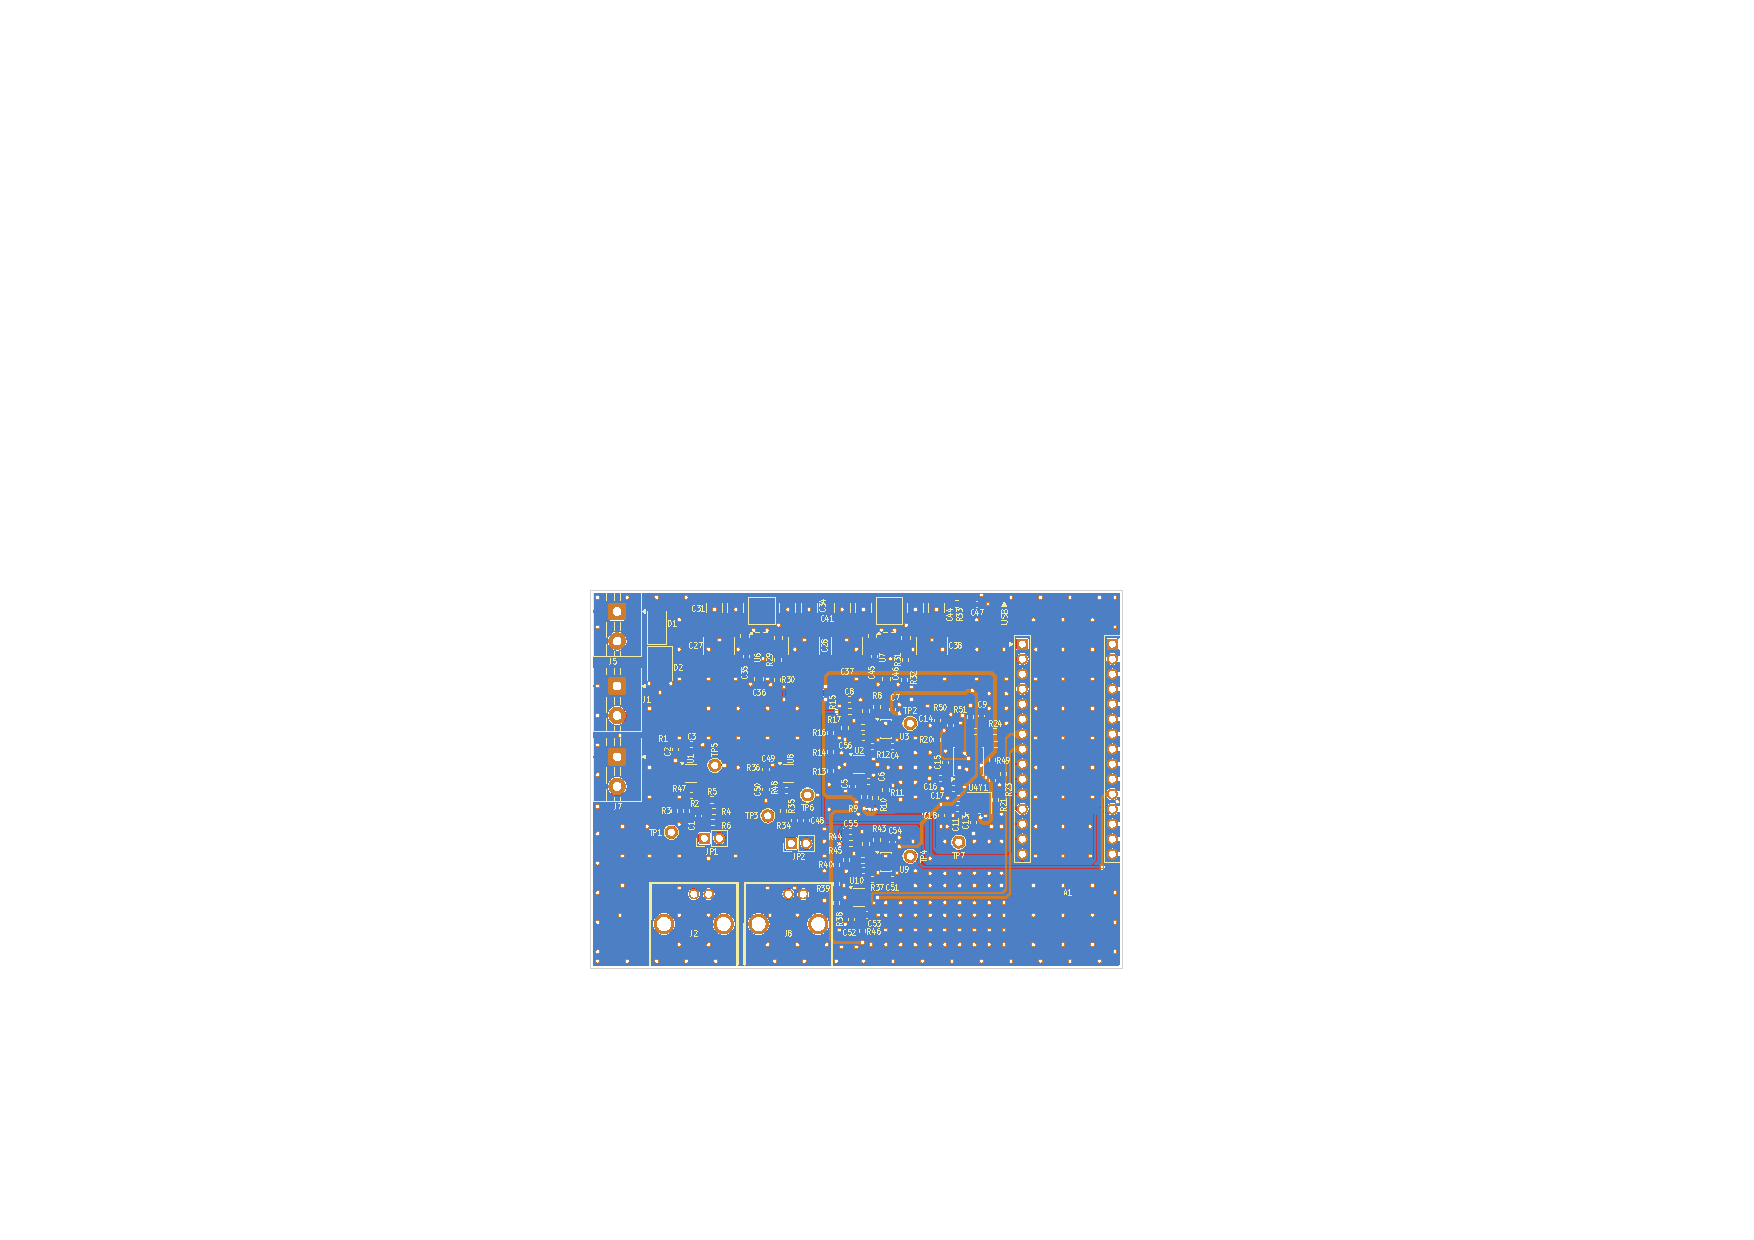
\includegraphics[width=0.78\linewidth]{figuras/placa_completa.pdf}\par
  \vspace{14mm}
  {\large Paso a paso: qué circuito es, qué piezas se usaron,\\ por qué la placa terminó en 4 capas y cómo se ruteó y se verificó.\par}
  \vfill
  {\large Universidad Nacional de Colombia, sede Manizales\par}
  {\large Noviembre de 2026\par}
  \vspace{4mm}
  {\small\color{grisnota} Fuente: rama \texttt{workspace/voxter}, carpeta \texttt{hardware/pcb/}.\par}
\end{titlepage}

\tableofcontents

\chapter[Introducción]{Introducción: qué es esta placa y cómo se diseñó}\label{cap:intro}

\textbf{En este capítulo vas a ver:}
\begin{itemize}
  \item Qué es un sonómetro y qué parte de él resuelve esta placa.
  \item Qué es un micrófono IEPE, explicado desde cero, y por qué hay que alimentarlo con corriente constante.
  \item El diagrama de bloques de toda la placa, con los nombres de red que vas a encontrar en KiCad.
  \item De dónde salió el diseño (Altium del equipo $\rightarrow$ KiCad Rev~B) y el flujo de trabajo completo hasta los archivos de JLCPCB.
  \item Cómo leer el resto del documento: las cajas de colores y las etiquetas que dicen de dónde sale cada dato.
\end{itemize}

\section{El problema: medir sonido con un micrófono de medición}

Un \textbf{sonómetro} es un instrumento que mide la presión sonora: cuánto varía la presión del aire alrededor de la presión atmosférica cuando pasa una onda de sonido. Esa variación se mide en pascales (\si{\pascal}) y normalmente se expresa en decibeles de nivel de presión sonora (\si{\decibel} SPL). Un sonómetro completo tiene tres partes:
\begin{enumerate}
  \item Un \textbf{micrófono de medición}, que convierte presión en voltaje con una sensibilidad conocida. Por ejemplo, \SI{50}{\milli\volt\per\pascal} quiere decir que \SI{1}{\pascal} de presión da \SI{50}{\milli\volt} de señal.
  \item Una \textbf{etapa analógica} (el \emph{front end}), que alimenta el micrófono, extrae la señal y la acomoda al rango del convertidor.
  \item Un \textbf{convertidor analógico--digital} y un procesador, que digitalizan la señal y calculan lo que haga falta (forma de onda, nivel en dB, ponderación A, etc.).
\end{enumerate}

Esta placa resuelve las partes~2 y~3 para \textbf{dos micrófonos distintos}, uno por canal:

\begin{center}
\begin{tabularx}{\linewidth}{@{}L{0.17\linewidth}L{0.33\linewidth}Y@{}}
\toprule
\textbf{Canal} & \textbf{Micrófono} & \textbf{Datos que importan para la placa}\\
\midrule
CH1 (\net{J2}) & ROGA Instruments RG-50 (¼'', electret prepolarizado con IEPE integrado) & Corriente de \SIrange{2}{20}{\milli\ampere}, alimentación de \SIrange{18}{30}{\volt}, polarización de salida de \SI{12.5}{\volt}, sensibilidad nominal de \SI{50}{\milli\volt\per\pascal}, máximo \SI{130}{\decibel} pico ($\approx$\,\SI{3.2}{\volt} pico) \doc{ROGA RG-50}\\
CH2 (\net{J8}) & Svantek SV~12 (preamplificador IEPE de ½'', con cápsula aparte) & Alimentación ``IEPE type -- \SI{1.5}{\milli\ampere} @ \SI{30}{\volt}'', excursión de salida $\geq$\,\SI{10.8}{\volt} pico. La polarización de DC no está publicada \doc{Svantek SVAN 977W App.~C}\\
\bottomrule
\end{tabularx}
\end{center}

La identificación exacta de los dos micrófonos todavía no está confirmada con el objeto en la mano (conector TNC del SV~12, modelo exacto del ROGA). El capítulo~\ref{cap:banco} lo deja en la lista de cosas por verificar.

\section{Qué es un micrófono IEPE}\label{sec:c01-iepe}

IEPE significa \emph{Integrated Electronics Piezo-Electric}. Es un estándar de la industria de sensores (acelerómetros y micrófonos de medición) en el que el sensor trae adentro un pequeño amplificador. Lo interesante es que \textbf{la alimentación y la señal viajan por el mismo cable coaxial de dos conductores}: el centro y la malla.

\begin{idea}[cómo funciona IEPE]
\begin{enumerate}
  \item Desde afuera se le inyecta al sensor una \textbf{corriente constante} $I_0$, típicamente de \SIrange{2}{20}{\milli\ampere}, tomada de una fuente de \SIrange{18}{30}{\volt}.
  \item El amplificador interno del sensor ``se acomoda'' y fija en su salida un voltaje de DC llamado \textbf{polarización} $V_B$ (en inglés \emph{bias}), que suele estar entre \SIrange{8}{14}{\volt}.
  \item Cuando llega sonido, el amplificador mueve ese voltaje hacia arriba y hacia abajo. La señal acústica es una \textbf{tensión AC montada encima de la polarización de DC}:
  \begin{equation}
    v(t) = V_B + S\cdot p(t)
    \label{eq:c01-iepe}
  \end{equation}
  donde $S$ es la sensibilidad (\si{\volt\per\pascal}) y $p(t)$ la presión acústica (\si{\pascal}).
\end{enumerate}
Como la corriente es constante, el cable no ``ve'' cambios de corriente: toda la información está en el voltaje del nodo. Por eso basta un coaxial con un conector BNC.
\end{idea}

La figura~\ref{fig:c01-iepe} muestra el modelo eléctrico. Del lado de la placa hay una fuente de corriente; del lado del micrófono, el amplificador interno se puede ver como una fuente de DC $V_B$ en serie con la señal $S\,p(t)$ y con una resistencia de salida pequeña $R_o$ (en el RG-50, menos de \SI{50}{\ohm} \doc{ROGA RG-50}).

\begin{figure}[htbp]
\centering
\begin{circuitikz}[scale=0.95, transform shape]
  % fuente de corriente de la placa
  \draw (0,5.2) node[above]{$+\SI{24}{\volt}$} to[short,o-] (0,4.6)
        to[american current source, l_=$I_0$] (0,2.4) coordinate (n);
  \draw (n) to[short,*-o] (2.4,2.4) node[above]{BNC};
  \draw (2.4,2.4) -- (4.6,2.4);
  % modelo del sensor
  \draw (4.6,2.4) to[R, l=$R_o$] (4.6,0.8)
        to[sinusoidal voltage source, l=$S\,p(t)$] (4.6,-0.8)
        to[battery1, l=$V_B$, invert] (4.6,-2.4) -- (4.6,-2.8) node[ground]{};
  \draw[dashed, rounded corners, verdeplaca] (3.3,2.9) rectangle (6.4,-2.6);
  \node[verdeplaca, align=center, font=\footnotesize] at (4.85,3.35) {micrófono IEPE\\(amplificador interno)};
  % voltaje del nodo
  \draw (n) -- (-1.6,2.4);
  \draw (-1.6,2.4) to[open, v^>=$v(t)$] (-1.6,-2.4);
  \draw (-1.6,-2.4) -- (-1.6,-2.8) node[ground]{};
  \node[draw=cobre, fill=cobre!6, align=left, font=\footnotesize, anchor=west] at (0.4,0.2)
       {$v(t)=V_B+S\,p(t)$\\[2pt]DC de \SIrange{8}{14}{\volt}\\+ AC de mV a V};
  \node[font=\footnotesize, align=right, anchor=east] at (-0.7,3.5) {fuente de corriente\\de la placa (LT3092)};
\end{circuitikz}
\caption{Modelo de un canal IEPE. La placa inyecta una corriente constante $I_0$; el amplificador del micrófono fija la polarización $V_B$ y le suma la señal. Todo lo que hay que medir está en el voltaje $v(t)$ del nodo, que en la placa se llama \net{IEPE} (CH1) o \net{IEPE_SV} (CH2).}
\label{fig:c01-iepe}
\end{figure}

Para que veas los órdenes de magnitud: con el RG-50 ($S=\SI{50}{\milli\volt\per\pascal}$, $V_B=\SI{12.5}{\volt}$), un tono de \SI{94}{\decibel} SPL, que equivale a \SI{1}{\pascal} eficaz, da una señal de \SI{50}{\milli\volt} eficaces ($\approx$\,\SI{71}{\milli\volt} pico) encima de \SI{12.5}{\volt} de DC. La figura~\ref{fig:c01-onda} lo dibuja con la señal exagerada para que se vea.

\begin{figure}[htbp]
\centering
\begin{tikzpicture}
\begin{axis}[width=0.8\linewidth, height=4.6cm, xlabel={tiempo (ms)}, ylabel={$v(t)$ (V)},
  ymin=0, ymax=16.5, xmin=0, xmax=3, grid=both, grid style={gray!20},
  ytick={0,5,10,12.5,15}, yticklabels={0,5,10,{12,5},15},
  xticklabel style={/pgf/number format/use comma}]
  \addplot[domain=0:3, samples=200, thick, verdeplaca] {12.5 + 1.2*sin(deg(2*pi*x))};
  \addplot[domain=0:3, dashed, cobre, thick] {12.5};
  \node[cobre, font=\footnotesize, anchor=south west] at (axis cs:0.05,14.1) {polarización $V_B$ (DC)};
  \node[verdeplaca, font=\footnotesize, anchor=north west] at (axis cs:0.05,10.6) {señal $S\,p(t)$ (AC), aquí exagerada};
\end{axis}
\end{tikzpicture}
\caption{Lo que hay en el nodo IEPE: una tensión de DC grande con la señal acústica montada encima. El trabajo de la etapa analógica es quitar la DC y quedarse con la AC, sin perder información.}
\label{fig:c01-onda}
\end{figure}

\begin{ojo}[reglas de seguridad de IEPE]
Las guías de PCB Piezotronics resumidas en \archivo{AGENTS.md} §4 dan reglas que la placa respeta:
\begin{itemize}
  \item nunca más de \SI{30}{\volt} ni más de \SI{20}{\milli\ampere} sobre el sensor;
  \item nunca aplicar tensión sin limitar la corriente;
  \item nunca \SI{48}{\volt} de alimentación \emph{phantom} ni \SI{200}{\volt} de polarización de cápsula;
  \item cada sensor con su propia fuente de corriente: \textbf{nunca dos sensores IEPE en paralelo}.
\end{itemize}
Por eso la placa tiene dos fuentes de corriente independientes (\net{U1} y \net{U8}) y la entrada de \SI{24}{\volt} pasa por un TVS que recorta los picos (capítulo~\ref{cap:alim}).
\end{ojo}

Un dato útil para depurar: la polarización $V_B$ te dice el estado del sensor. Cerca de \SI{0}{\volt} indica un cortocircuito; cerca de la tensión máxima de la fuente indica un circuito abierto o un sensor muerto; entre \SIrange{7}{14}{\volt} el sensor está bien \copia[(PCB G0001E, vía AGENTS.md §4)].

\section{La placa completa en un diagrama de bloques}\label{sec:c01-bloques}

La placa tiene dos partes que conviene mirar por separado: el árbol de alimentación (figura~\ref{fig:c01-potencia}) y la cadena de señal de un canal (figura~\ref{fig:c01-bloques}). Los dos canales son iguales; cambian los designadores y el sufijo \net{_SV} de las redes del canal~2.

\begin{figure}[htbp]
\centering
\begin{tikzpicture}[
  blq/.style={draw, rounded corners=2pt, align=center, font=\footnotesize, minimum height=11mm, minimum width=26mm, fill=white},
  pot/.style={blq, fill=cobre!8, draw=cobre},
  carga/.style={align=left, font=\scriptsize, anchor=west},
  red/.style={font=\scriptsize\ttfamily, inner sep=1.5pt},
  flecha/.style={-{Stealth[length=2mm]}, thick}]
  \node[pot] (j5) at (0,0) {Entrada \SI{24}{\volt}\\\net{J5}};
  \node[pot] (prot) at (3.5,0) {Protección\\\net{D1} SS34\\\net{D2} SMBJ26A};
  \node[pot] (b3) at (7.5,1.9) {Buck \SI{3.3}{\volt}\\\net{U6} LMR36015};
  \node[pot] (b5) at (7.5,0) {Buck \SI{5}{\volt}\\\net{U7} LMR36015};
  \node[pot] (en) at (7.5,-1.9) {Habilitación\\\net{J1} / \net{J7}};
  \node[pot, minimum width=17mm] (rc) at (10.4,0) {RC\\\net{R33}+\net{C47}};
  \draw[flecha] (j5) -- node[red,above]{24V\_IN} (prot);
  \draw[thick] (prot.east) -- node[red,above,pos=0.45]{24V\_PROT} (5.6,0);
  \draw[thick] (5.6,1.9) -- (5.6,-1.9);
  \fill (5.6,0) circle (1.4pt);
  \draw[flecha] (5.6,1.9) -- (b3.west);
  \draw[flecha] (5.6,0) -- (b5.west);
  \draw[flecha] (5.6,-1.9) -- (en.west);
  \draw[flecha] (b5) -- node[red,above]{5V} (rc);
  \draw[flecha] (b3.east) -- node[red,above]{3V3} (11.4,1.9);
  \draw[flecha] (rc.east) -- node[red,above]{5V\_A} (12.2,0);
  \draw[flecha] (en.east) -- node[red,above]{IEPE\_FEED} (11.4,-1.9);
  \node[carga] at (11.5,1.9) {ADC (VDD), DAC $\times2$,\\oscilador, pull-ups I$^2$C};
  \node[carga] at (12.3,0) {op-amps $\times2$,\\ADC (VCC)};
  \node[carga] at (11.5,-1.9) {fuentes IEPE\\\net{U1} / \net{U8}};
\end{tikzpicture}
\caption{Árbol de alimentación. Todo sale de los \SI{24}{\volt} protegidos (\net{24V_PROT}). La NUCLEO no se alimenta de esta placa: usa su propio USB (capítulo~\ref{cap:alim}).}
\label{fig:c01-potencia}
\end{figure}

\begin{figure}[htbp]
\centering
\begin{tikzpicture}[
  blq/.style={draw, rounded corners=2pt, align=center, font=\footnotesize, minimum height=12mm, text width=25mm, fill=white},
  ana/.style={blq, fill=azulidea!7, draw=azulidea},
  dig/.style={blq, fill=verdeplaca!8, draw=verdeplaca},
  red/.style={font=\scriptsize\ttfamily, inner sep=1.5pt},
  flecha/.style={-{Stealth[length=2mm]}, thick}]
  \node[ana] (src) at (0,0) {Fuente IEPE\\\net{U1} LT3092};
  \node[ana] (bnc) at (0,-2.6) {Micrófono\\BNC \net{J2}};
  \node[ana] (sum) at (4.4,0) {Sumador inversor\\\net{U3A} TLV9152};
  \node[ana] (seg) at (4.4,-2.6) {Filtro \net{R12}/\net{C4}\\+ seguidor \net{U3B}};
  \node[ana] (adc) at (8.8,0) {ADC 24 bits\\\net{U4} PCM1808};
  \node[dig] (dac) at (8.8,-2.6) {DAC 12 bits\\\net{U2} MCP4725};
  \node[dig] (y1) at (8.8,2.3) {Oscilador \net{Y1}\\\SI{24.576}{\mega\hertz}};
  \node[dig] (nuc) at (13.2,0) {NUCLEO-L432KC\\\net{A1}};
  \node[dig] (pc) at (13.2,2.3) {PC (Python)};
  \draw[flecha] (0,1.75) node[red,above]{IEPE\_FEED (de J1)} -- (src.north);
  \draw[thick, {Stealth[length=2mm]}-{Stealth[length=2mm]}] (src) -- node[red,right]{IEPE} (bnc);
  \draw[flecha] (src) -- node[red,above]{IEPE} (sum);
  \draw[flecha] (sum) -- node[red,above]{REST\_OUT} (adc);
  \draw[flecha] (y1) -- node[red,right]{MCLK} (adc);
  \draw[flecha] (adc) -- node[red,above]{SAI} (nuc);
  \draw[flecha] (nuc) -- node[red,right]{USB} (pc);
  \draw[flecha] (nuc.south) |- node[red,pos=0.75,above]{I2C} (dac.east);
  \draw[flecha] (dac) -- node[red,above]{DAC\_RAW} (seg);
  \draw[flecha] (seg) -- node[red,right]{VSHIFT} (sum);
  \draw[flecha] (6.6,0) -- (6.6,-1.25) -- node[red,below,pos=0.45]{DC\_MON (divisor R15/R17)} (12.4,-1.25) -- (12.4,-0.62);
  \fill (6.6,0) circle (1.4pt);
\end{tikzpicture}
\caption{Cadena de señal de un canal con los nombres de red de KiCad (canal~1). En el canal~2 las piezas son \net{U8}, \net{J8}, \net{U9}, \net{U10} y las redes llevan el sufijo \net{_SV} (\net{IEPE_SV}, \net{REST_SV}, \net{DC_MON2}\ldots). Los dos canales comparten el ADC estéreo \net{U4}, el oscilador y la NUCLEO. La flecha de abajo es el lazo de DC: la NUCLEO mide la DC de la salida y corrige \net{VSHIFT} con el DAC.}
\label{fig:c01-bloques}
\end{figure}

Recorramos las dos figuras siguiendo la energía y la señal:

\begin{enumerate}
  \item \textbf{Alimentación} (capítulo~\ref{cap:alim}). Entran \SI{24}{\volt} de la fuente de laboratorio por la bornera \net{J5}. Un diodo en serie protege contra la polaridad invertida y un TVS recorta los picos; desde ahí la red se llama \net{24V_PROT}. Dos convertidores conmutados (\emph{bucks}) sacan \SI{3.3}{\volt} y \SI{5}{\volt}, y un filtro RC limpia los \SI{5}{\volt} para la parte analógica (\net{5V_A}).
  \item \textbf{Fuente IEPE} (capítulo~\ref{cap:analog}). Cada canal toma \net{24V_PROT} a través de un puente (\net{J1} o \net{J7}), y un regulador LT3092 configurado como fuente de corriente alimenta al micrófono por el BNC.
  \item \textbf{Sumador inversor}. El nodo IEPE (DC + AC) entra por una cadena de resistencias de \SI{1}{\mega\ohm} a un amplificador inversor que le resta un voltaje de referencia ajustable (\net{VSHIFT}). La salida, \net{REST_OUT}, queda con la DC llevada a un nivel conocido y la AC atenuada unas 10 veces.
  \item \textbf{Lazo de DC}. La NUCLEO mide la DC de la salida (\net{DC_MON}) y corrige \net{VSHIFT} con un DAC MCP4725 por I$^2$C. Así la salida se mantiene centrada aunque cambie la polarización del micrófono.
  \item \textbf{ADC} (capítulo~\ref{cap:digital}). Un PCM1808 de 24 bits digitaliza los dos canales a \SI{48}{\kilo\hertz}, con su reloj de \SI{24.576}{\mega\hertz}, y los manda a la NUCLEO por I$^2$S (periférico SAI del STM32).
  \item \textbf{NUCLEO-L432KC y PC}. La tarjeta NUCLEO va enchufada en un zócalo (\net{A1}). Recibe el audio, corre el lazo de DC y manda los datos al PC por su USB.
\end{enumerate}

\begin{idea}[por qué no se usa un simple condensador de acople]
La forma clásica de quitar la DC de un IEPE es un condensador en serie y una resistencia a tierra (un filtro pasa-altos). El profesor objetó la versión~1 de la propuesta precisamente por la fase que mete ese condensador y por el offset ``sin referencia definida'' (\archivo{AGENTS.md} §10). El circuito del equipo, que es el que se usa en esta placa, es \textbf{acoplado en DC}: resta una referencia conocida (\net{VSHIFT}) que un lazo digital ajusta. El capítulo~\ref{cap:analog} lo explica con las ecuaciones.
\end{idea}

\section{De dónde viene el diseño}\label{sec:c01-origen}

El diseño no se hizo desde cero en KiCad. Tiene una historia que conviene conocer, porque explica por qué algunas piezas están como están:

\begin{enumerate}
  \item \textbf{Rev~A, el circuito del equipo en Altium} (\archivo{hardware/Sonometro_2CH/*.SchDoc}). Tenía el canal~1 completo (fuente IEPE, AFE, DAC, ADC y un STM32 soldado), pero le faltaban la alimentación de \SI{24}{\volt}, los bucks y el canal~2.
  \item \textbf{Lo que faltaba} salió de \archivo{hardware/docs/connection_matrix.md}: la entrada de \SI{24}{\volt}, los dos LMR36015, el filtro de \net{5V_A} y el canal~2 como espejo pieza por pieza del canal~1.
  \item \textbf{Rev~B, la reconstrucción en KiCad.} Un script lee los \archivo{.SchDoc} binarios de Altium, saca la conectividad real y arma una netlist objetivo en \archivo{tools/design.py}. Ese archivo es la \textbf{fuente única de verdad}: cada pieza tiene su valor, su footprint, su código de fabricante (MPN), su código LCSC y el motivo de cada cambio. De ahí se generan el esquemático (\archivo{tools/gen_sch_wired.py}) y la lista \archivo{tools/target.json}, contra la que se verifica todo.
  \item \textbf{Cambios C1--C17.} Sobre el circuito del equipo se hicieron 17 cambios, cada uno con su justificación y su fuente: la NUCLEO enchufada en lugar del STM32 soldado (C1--C2), el oscilador de \SI{24.576}{\mega\hertz} (C3), la protección de entrada (C4), los BNC (C8), el condensador de realimentación de \SI{10}{\pico\farad} (C16), el cambio de piezas por stock de JLCPCB (C17), entre otros. El capítulo~\ref{cap:piezas} los explica uno por uno.
\end{enumerate}

El resultado es una placa de \SI{90}{\milli\meter} $\times$ \SI{64}{\milli\meter} con \textbf{127 piezas y 68 redes con nombre}, de 4 capas, para fabricar y ensamblar en JLCPCB.

\section{El flujo de trabajo, paso a paso}\label{sec:c01-flujo}

Diseñar una PCB no es ``dibujar pistas''. Es una cadena de pasos donde cada uno se verifica antes del siguiente. La figura~\ref{fig:c01-flujo} muestra el que se siguió.

\begin{figure}[htbp]
\centering
\begin{tikzpicture}[
  paso/.style={draw=verdeplaca, fill=verdeplaca!6, rounded corners=2pt, align=left, font=\footnotesize,
    text width=0.78\linewidth, inner sep=5pt},
  num/.style={circle, fill=cobre, text=white, font=\footnotesize\bfseries, minimum size=6mm, inner sep=0pt},
  node distance=2.5mm]
  \node[paso] (p1) {\textbf{Esquemático y netlist.} \archivo{design.py} $\to$ \archivo{target.json} $\to$ \archivo{pcb.kicad_sch}. Verificación: ERC 0 y comparación pin a pin contra \archivo{target.json} (\archivo{verify.py}).};
  \node[paso, below=of p1] (p2) {\textbf{Reglas.} Capacidades de JLCPCB leídas de sus páginas, reglas de los datasheets y notas de aplicación, todo con fuente en \archivo{REGLAS.md}. Se cargan en KiCad: restricciones de placa, clases de red y reglas propias en \archivo{pcb.kicad_dru}.};
  \node[paso, below=of p2] (p3) {\textbf{Selección y auditoría de piezas.} Stock en JLCPCB, piezas \emph{basic} o \emph{extended}, footprint comparado con el de la pieza exacta (\archivo{fabricacion/auditoria_piezas.md}).};
  \node[paso, below=of p3] (p4) {\textbf{Placement.} Ubicación por bloques, zona analógica y zona digital; cambios solo con aprobación.};
  \node[paso, below=of p4] (p5) {\textbf{Decisión de capas.} Prueba de factibilidad (el ``oráculo'' con Freerouting en copias): con 2 capas no había solución limpia $\to$ 4 capas.};
  \node[paso, below=of p5] (p6) {\textbf{Ruteo por bloques} (bucks, entrada, fuentes IEPE, ADC, AFE, analógicas largas, digital, alimentación, tierra, teardrops y serigrafía). Al final de \emph{cada} bloque: DRC con paridad, ERC, chequeo propio (\archivo{revisar_pistas.py}), imágenes de las capas y commit.};
  \node[paso, below=of p6] (p7) {\textbf{Cálculos sobre la placa ruteada.} Anchos de pista, caídas de tensión, vías, temperaturas y tiempos del buck, medidos sobre el archivo real (\archivo{CALCULOS.md}).};
  \node[paso, below=of p7] (p8) {\textbf{Fabricación.} Gerber, taladros, BOM y CPL con las rotaciones corregidas; revisión de los Gerber con una biblioteca externa (gerbonara) y consulta del stock del día (\archivo{fabricacion/}).};
  \foreach \i in {1,...,8} { \node[num, left=3mm of p\i] {\i}; }
  \foreach \i/\j in {1/2,2/3,3/4,4/5,5/6,6/7,7/8} { \draw[-{Stealth[length=2mm]}, cobre, thick] (p\i.south) -- (p\j.north); }
\end{tikzpicture}
\caption{Flujo de trabajo seguido para la placa. Ningún paso se dio por bueno sin una verificación con herramienta.}
\label{fig:c01-flujo}
\end{figure}

\begin{idea}[por qué rutear ``por bloques'' y verificar cada vez]
Si ruteas toda la placa de una y al final el DRC te da 300 errores, no sabes cuál de tus decisiones los causó. Si ruteas un bloque (por ejemplo, solo las fuentes conmutadas), lo verificas y haces commit, cualquier error nuevo en el bloque siguiente es culpa del bloque siguiente. Además, cada commit es un punto al que puedes volver. Es lo mismo que probar un programa función por función en lugar de escribirlo entero y compilar al final.
\end{idea}

\begin{decision}[definición de ``terminado'']
\textbf{Qué se decidió:} la placa solo se considera terminada con DRC en 0 errores, 0 conexiones sin rutear, 0 hallazgos del chequeo propio y cada advertencia explicada.\\
\textbf{Alternativas:} excluir violaciones o bajar severidades en KiCad para que el DRC ``pase''.\\
\textbf{Por qué:} una violación excluida sigue estando en la placa. La regla del proyecto fue explícita: prohibido excluir violaciones o bajar severidades. Lo que no cumple una regla y se acepta queda escrito como excepción, con su motivo (capítulo~\ref{cap:banco}).\\
\textbf{Fuente:} especificación del ruteo dada por el dueño del proyecto; estado final en \archivo{PLAN_RUTEO.md} §17.
\end{decision}

\section{Mapa de archivos del repositorio}\label{sec:c01-archivos}

Todo vive en la rama \archivo{workspace/voxter}, carpeta \archivo{hardware/pcb/}. Estos son los archivos que vas a necesitar:

\begin{longtable}{@{}L{0.37\linewidth}L{0.59\linewidth}@{}}
\toprule
\textbf{Archivo o carpeta} & \textbf{Para qué sirve}\\
\midrule\endhead
\archivo{pcb.kicad_sch}, \archivo{pcb.kicad_pcb}, \archivo{pcb.kicad_pro} & El esquemático, la placa y el proyecto de KiCad~10.\\
\archivo{pcb.kicad_dru} & Reglas de diseño propias (separaciones especiales, vías tapadas lejos de los pads, etc.).\\
\archivo{lib/} & Biblioteca local: símbolos y footprints que no están en KiCad o que se corrigieron (RNX del LMR36015, TSOT-23-8 de ADI, BNC, NUCLEO).\\
\archivo{REGLAS.md} & Todas las reglas de diseño con su fuente: capacidades de JLCPCB, reglas de cada integrado, tierra, IPC.\\
\archivo{CALCULOS.md} & Cálculos generados desde la placa ruteada (\archivo{tools/calculos.py}).\\
\archivo{PLAN_RUTEO.md} & La bitácora: decisiones y verificaciones de cada bloque, en orden.\\
\archivo{tools/design.py}, \archivo{tools/target.json}, \archivo{tools/changes.json} & Netlist objetivo, la lista de piezas que sale de ella y los cambios C1--C17.\\
\archivo{tools/gen_sch_wired.py}, \archivo{tools/buildlib.py}, \archivo{tools/eco.py} & Generan el esquemático y la biblioteca, y aplican cambios a la placa sin borrar el ruteo.\\
\archivo{tools/verify.py}, \archivo{tools/config_reglas.py} & Verificación de la netlist y configuración de reglas y severidades.\\
\archivo{tools/ruteo/bloques/b1_bucks.py} \ldots{} \archivo{b9_gnd.py} & Un script por bloque de ruteo: puntos de paso de cada pista y cada vía.\\
\archivo{tools/ruteo/polilineas.py} & Convierte esos puntos de paso en pistas y vías reales de KiCad.\\
\archivo{tools/ruteo/revisar_pistas.py} & El chequeo propio (A--M): entrada a pads, desacoplos, vías GND, serigrafía sobre vías, etc.\\
\archivo{tools/ruteo/verificar_bloque.py} & Corre todo después de un bloque: zonas, DRC, ERC, paridad, chequeo propio, imágenes.\\
\archivo{tools/ruteo/cosido.py}, \archivo{teardrops.py}, \archivo{serigrafia.py} & Vías de cosido de tierra, teardrops y ubicación de designadores.\\
\archivo{tools/ruteo/oraculo/} & Las pruebas de factibilidad con Freerouting, hechas sobre copias.\\
\archivo{tools/analisis_opamp.py} & Estabilidad del sumador y región de transición del TLV9152.\\
\archivo{fabricacion/} & Gerber, taladros, BOM, CPL, rotaciones, piezas a mano, PDF de montaje, auditoría de piezas, stock y revisión de Gerber.\\
\bottomrule
\end{longtable}

\section{Cómo leer este documento}\label{sec:c01-leer}

\subsection*{Las cajas}
A lo largo del documento vas a encontrar cuatro tipos de caja:

\begin{idea}[ejemplo]
Un concepto explicado con palabras sencillas, antes de usarlo. Si ya lo conoces, te la puedes saltar.
\end{idea}

\begin{decision}[ejemplo]
\textbf{Qué se decidió}, \textbf{qué alternativas había}, \textbf{por qué} se eligió esa y \textbf{de dónde} sale el dato. Son las cajas más importantes: si alguien (por ejemplo, el profesor) pregunta ``¿por qué hicieron esto?'', la respuesta está aquí.
\end{decision}

\begin{calculo}[ejemplo]
Un cálculo paso a paso, con la ecuación, los números y el resultado. Por ejemplo, la frecuencia de corte del filtro de \net{5V_A}:
$f_c = \dfrac{1}{2\pi R C} = \dfrac{1}{2\pi\cdot\SI{10}{\ohm}\cdot\SI{10}{\micro\farad}} \approx \SI{1.59}{\kilo\hertz}$.
\end{calculo}

\begin{ojo}[ejemplo]
Un error típico, una advertencia o algo que quedó sin verificar.
\end{ojo}

\subsection*{Las etiquetas de origen}
Cada dato numérico lleva al lado una etiqueta que dice de dónde salió. Esto es importante: un número sin origen no se puede defender.

\begin{center}
\begin{tabularx}{\linewidth}{@{}L{0.25\linewidth}Y@{}}
\toprule
\textbf{Etiqueta} & \textbf{Qué significa y ejemplo}\\
\midrule
\doc{SNVSB49D p.6} & Leído del datasheet o de la página del fabricante, con el documento y la página. Ejemplo: la tensión de realimentación del LMR36015 es \SIrange{0.985}{1.015}{\volt} \doc{SNVSB49D p.6}.\\
\copia & Tomado de una fuente secundaria (una copia del datasheet, un resumen) y no contrastado con el original. Ejemplo: la tensión de ruptura mínima del SMBJ26A es \SI{28.9}{\volt} \copia.\\
\estimado & Un supuesto de diseño. Ejemplo: el oscilador consume como mucho \SI{10}{\milli\ampere} \estimado.\\
\medido & Medido por un script sobre el archivo de KiCad (no en el laboratorio). Ejemplo: la separación mínima de las redes de \SI{24}{\volt} es \SI{0.200}{\milli\meter} \medido.\\
\medir & Algo que solo se confirma midiendo la placa real en el banco. Ejemplo: el consumo de cada buck sin carga \medir.\\
\bottomrule
\end{tabularx}
\end{center}

\subsection*{Nombres}
Las redes, las piezas y los pines se escriben en letra de máquina, igual que en KiCad: \net{IEPE_SV} es una red, \net{U3} una pieza y \net{U3.8} el pin~8 de \net{U3}. Las capas de la placa se escriben \capa{F.Cu} (cobre superior), \capa{In1.Cu} y \capa{In2.Cu} (internas) y \capa{B.Cu} (cobre inferior). Las coordenadas están en milímetros, en el sistema de KiCad (origen arriba a la izquierda de la hoja, Y hacia abajo).

\subsection*{Orden recomendado de lectura}
Si tienes poco tiempo: este capítulo, el~\ref{cap:capas} (por qué 4 capas) y el~\ref{cap:banco} (excepciones y pendientes). Si vas a defender el diseño frente al profesor, lee los capítulos~\ref{cap:alim} a~\ref{cap:digital}, que explican el circuito, y el~\ref{cap:calculos}, que tiene los números.

\section*{Resumen}
\begin{itemize}
  \item La placa es el \emph{front end} y el digitalizador de un sonómetro de dos canales: CH1 para un ROGA RG-50 y CH2 para un Svantek SV~12, los dos IEPE.
  \item Un sensor IEPE se alimenta con corriente constante por el mismo coaxial por el que sale la señal. En el nodo hay $v(t)=V_B+S\,p(t)$: una DC grande con la señal acústica encima.
  \item La cadena es: \SI{24}{\volt} protegidos $\to$ bucks de \SI{3.3}{\volt} y \SI{5}{\volt} $\to$ fuente IEPE LT3092 $\to$ sumador inversor que resta \net{VSHIFT} $\to$ PCM1808 $\to$ NUCLEO $\to$ PC. Un lazo digital (DAC + \net{DC_MON}) mantiene la DC de la salida en su sitio.
  \item El diseño parte del Altium del equipo, se reconstruyó en KiCad desde \archivo{tools/design.py} y tiene 17 cambios documentados.
  \item El trabajo siguió un flujo con verificación en cada paso; ``terminado'' quiere decir DRC, ERC y paridad en 0 sin excluir nada.
\end{itemize}

\chapter[Alimentación]{Alimentación: de \SI{24}{\volt} a \SI{3.3}{\volt}, \SI{5}{\volt} y 5V\_A}\label{cap:alim}

\textbf{En este capítulo vas a ver:}
\begin{itemize}
  \item Cuánta energía necesita cada parte de la placa (el presupuesto de consumo).
  \item Cómo se protege la entrada de \SI{24}{\volt}: diodo en serie contra polaridad invertida y TVS contra picos.
  \item Qué es un convertidor \emph{buck}, explicado desde cero, y por qué se usa en lugar de un regulador lineal.
  \item Por qué se eligió el LMR36015 en su variante FPWM de \SI{1}{\mega\hertz}, y cuánto cuesta esa decisión.
  \item El cálculo de cada pieza externa de los bucks: divisor de realimentación, bobina, condensadores.
  \item La comprobación de los tiempos mínimos de encendido y apagado en el peor caso.
  \item El filtro RC que produce el riel analógico \net{5V_A} y por qué existe.
  \item Cómo se alimenta la NUCLEO y en qué orden se enciende todo.
\end{itemize}

\section{Qué hay que alimentar: el presupuesto de consumo}\label{sec:c02-presupuesto}

Antes de elegir una sola pieza de la fuente hay que saber cuánta corriente pide cada riel. La placa tiene cuatro redes de alimentación:

\begin{itemize}
  \item \net{24V_PROT}: los \SI{24}{\volt} de la fuente de laboratorio, ya protegidos. Alimenta los dos bucks y las dos fuentes de corriente IEPE.
  \item \net{3V3}: \SI{3.3}{\volt} para lo digital y los convertidores: la parte digital del ADC (VDD del PCM1808), los dos DAC MCP4725, el oscilador y las resistencias de pull-up del bus I$^2$C.
  \item \net{5V}: la salida del buck de \SI{5}{\volt}. Solo alimenta el filtro RC que produce \net{5V_A}.
  \item \net{5V_A}: \SI{5}{\volt} ``analógicos'' y filtrados: los dos op-amps TLV9152 y la parte analógica del ADC (VCC del PCM1808).
\end{itemize}

La tabla~\ref{tab:c02-presupuesto} sale de la sección~1 de \archivo{CALCULOS.md}. Son \textbf{cotas superiores}: se toma el máximo del datasheet, no el típico, para que la fuente nunca quede corta.

\begin{table}[htbp]
\centering
\caption{Corrientes de diseño por riel (cotas superiores).}
\label{tab:c02-presupuesto}
\begin{tabularx}{\linewidth}{@{}L{0.13\linewidth}Y L{0.14\linewidth}@{}}
\toprule
\textbf{Riel} & \textbf{De dónde sale la corriente} & \textbf{Total}\\
\midrule
\net{5V_A} & PCM1808 ICC máx. \SI{11}{\milli\ampere} \doc{SLES177B p.6} + 2 TLV9152, cada uno con 2 amplificadores a \SI{750}{\micro\ampere} máx. \doc{SBOS986E p.12} & \SI{14.0}{\milli\ampere}\\
\net{5V} & Solo alimenta a \net{5V_A} a través de \net{R33} & \SI{14.0}{\milli\ampere}\\
\net{3V3} & PCM1808 IDD \SI{10.2}{\milli\ampere} (a \SI{96}{\kilo\hertz}, el caso más alto) \doc{SLES177B p.6} + 2 MCP4725 a \SI{400}{\micro\ampere} máx. \doc{DS22039D p.3} + pull-ups I$^2$C + oscilador $\leq$\,\SI{10}{\milli\ampere} \estimado & \SI{22.4}{\milli\ampere}\\
\net{24V_PROT} & Se diseña con el límite de la fuente de banco (\SIrange{30}{50}{\milli\ampere}, \archivo{AGENTS.md} §5). Solo las fuentes IEPE piden como máximo \SI{3.98}{} + \SI{2.51}{\milli\ampere} & \SI{50}{\milli\ampere}\\
\bottomrule
\end{tabularx}
\end{table}

Fíjate en el orden de magnitud: \textbf{decenas de miliamperios}. Esta placa consume muy poco. Eso va a pesar en varias decisiones: los anchos de pista no los fija la corriente sino la fabricación (capítulo~\ref{cap:calculos}), y la eficiencia del buck en vacío importa más que su eficiencia a plena carga.

\begin{calculo}[cuánto le pide la placa a la fuente de \SI{24}{\volt}]
Sumemos la potencia de cada consumo, con las cotas de la tabla:
\begin{align*}
P_{3V3} &= \SI{3.3}{\volt}\cdot\SI{22.4}{\milli\ampere} \approx \SI{74}{\milli\watt}\\
P_{5V} &= \SI{5}{\volt}\cdot\SI{14.0}{\milli\ampere} = \SI{70}{\milli\watt}\\
P_{\text{bucks}} &\leq 2\cdot\SI{0.15}{\watt} = \SI{0.30}{\watt} \quad\text{(pérdidas en vacío, sección~\ref{sec:c02-fpwm})}\\
P_{\text{IEPE}} &\approx (\SI{3.98}{} + \SI{2.51}{\milli\ampere})\cdot\SI{23.5}{\volt} \approx \SI{0.15}{\watt}
\end{align*}
Total: unos \SI{0.6}{\watt}, que a \SI{23.5}{\volt} son unos \SI{25}{\milli\ampere} \estimado. Está por debajo de los \SIrange{30}{50}{\milli\ampere} a los que se limita la fuente de banco. Este número se confirma en el banco con el amperímetro \medir.
\end{calculo}

\section{La entrada: J5, D1 y D2}\label{sec:c02-entrada}

La figura~\ref{fig:c02-entrada} muestra la entrada. Los \SI{24}{\volt} llegan por la bornera \net{J5} (red \net{24V_IN}), pasan por el diodo \net{D1} y desde ahí la red se llama \net{24V_PROT}. Entre \net{24V_PROT} y tierra está el TVS \net{D2}. Este bloque no existía en el Altium del equipo: es el cambio C4 (capítulo~\ref{cap:piezas}).

\begin{figure}[htbp]
\centering
\begin{circuitikz}[scale=0.95, transform shape]
  \draw (0,2) node[left]{\net{J5.1}} to[short,o-] (0.6,2) node[above]{\net{24V_IN}} -- (1.2,2)
        to[sD, l=\net{D1} SS34] (3.6,2) coordinate (p);
  \draw (p) to[short,*-] (6.0,2) coordinate (q) to[short,*-] (8.4,2) node[right]{\net{24V_PROT} $\to$ bucks \net{U6}, \net{U7}};
  \node[above] at (4.8,2) {\net{24V_PROT}};
  \draw (p) to[zDo, l_=\net{D2} SMBJ26A, invert] (3.6,0) node[ground]{};
  \draw (q) -- (6.0,1.2) to[short,-o] (6.0,1.0) node[left]{\net{J1.1}};
  \node[font=\footnotesize, align=left, anchor=west] at (6.2,0.7) {bornera \net{J1} (y \net{J7})\\$\to$ \net{IEPE_FEED} $\to$ fuente IEPE};
  \draw (0,0) node[left]{\net{J5.2}} to[short,o-] (0.8,0) node[ground]{};
\end{circuitikz}
\caption{Entrada de alimentación. \net{D1} en serie bloquea la polaridad invertida; \net{D2} (TVS) recorta los picos sobre \net{24V_PROT}. \net{J1} y \net{J7} son borneras en serie con la alimentación de cada fuente IEPE.}
\label{fig:c02-entrada}
\end{figure}

\subsection{D1: protección contra polaridad invertida}

Si alguien conecta la fuente al revés, todos los integrados recibirían \SI{-24}{\volt}, y eso los mata. \net{D1} está \textbf{en serie}: con la polaridad correcta conduce; con la polaridad invertida queda en inversa y no deja pasar corriente.

Es un SS34, un diodo Schottky de \SI{40}{\volt} y \SI{3}{\ampere} \copia[(design.py)]. Se usa un Schottky porque cae menos tensión en directa que un diodo de silicio normal, unos \SI{0.4}{\volt} \estimado. Con la corriente de la placa, eso es nada:

\begin{calculo}[pérdida en D1]
$P_{D1} = I\cdot V_F = \SI{50}{\milli\ampere}\cdot\SI{0.4}{\volt} = \SI{20}{\milli\watt}$, menos de \SI{1}{\degreeCelsius} de calentamiento (\archivo{CALCULOS.md} §6). La consecuencia práctica es que a los bucks no les llegan \SI{24}{\volt} sino unos \SI{23.5}{\volt}. Por eso ese valor aparece en los cálculos de este capítulo.
\end{calculo}

\begin{decision}[diodo Schottky en serie]
\textbf{Qué se decidió:} un Schottky SS34 en serie con la entrada.\\
\textbf{Alternativas:} un MOSFET de canal P como ``diodo ideal'' (casi sin caída) o un diodo en paralelo con fusible (cortocircuita la fuente al invertirla).\\
\textbf{Por qué:} con \SI{50}{\milli\ampere} la caída del Schottky solo cuesta \SI{20}{\milli\watt}, y es una sola pieza \emph{basic} de JLCPCB (C8678). El MOSFET agrega piezas sin una ventaja que se note a este consumo.\\
\textbf{Fuente:} cambio C4 de \archivo{tools/design.py}; cálculo en \archivo{CALCULOS.md} §6.
\end{decision}

\subsection{D2: el TVS contra picos}

\begin{idea}[qué es un TVS]
Un TVS (\emph{Transient Voltage Suppressor}) es un diodo hecho para absorber picos de tensión. Mientras la tensión está por debajo de su \textbf{tensión de trabajo} $V_{RWM}$ casi no conduce (solo una corriente de fuga pequeña). Si un pico supera su \textbf{tensión de ruptura} $V_{BR}$, conduce mucho y ``se come'' la energía del pico, con la tensión sujeta cerca de su \textbf{tensión de recorte} (\emph{clamping}). Va en paralelo con la línea que protege, de la red a tierra. Es como una válvula de alivio en una tubería: cerrada en condiciones normales, se abre si la presión se dispara.
\end{idea}

El SMBJ26A tiene $V_{RWM}=\SI{26}{\volt}$ y $V_{BR}\geq\SI{28.9}{\volt}$ \copia. ¿Por qué 26?
\begin{itemize}
  \item Tiene que quedar \textbf{por encima} de los \SI{24}{\volt} normales con margen. Si su $V_{RWM}$ fuera menor que la tensión de trabajo, conduciría todo el tiempo y se calentaría.
  \item Tiene que quedar \textbf{por debajo} de lo que aguantan las piezas que protege. Los LMR36015 aceptan hasta \SI{60}{\volt} de entrada \doc{SNVSB49D p.1}, así que el recorte transitorio del TVS (unos \SI{42}{\volt} \copia[(REGLAS.md §5)]) no los pone en riesgo.
\end{itemize}

Como \net{D2} va después de \net{D1}, con la polaridad invertida el TVS no ve nada: \net{D1} ya bloqueó.

\begin{ojo}[valores del TVS sin datasheet a mano]
Los valores del SMBJ26A son los típicos de la serie SMBJ y vienen de una copia, no del datasheet del fabricante exacto (\archivo{CALCULOS.md} §1). En la práctica: no alimentes la placa con más de \SI{26}{\volt} continuos. El TVS también fija una tensión máxima de la que se parte para calcular separaciones entre pistas y tiempos del buck (sección~\ref{sec:c02-tiempos} y capítulo~\ref{cap:calculos}).
\end{ojo}

\subsection{J1 y J7: la habilitación de cada canal}

Cada fuente IEPE toma \net{24V_PROT} a través de una bornera de dos pines, \net{J1} (CH1) o \net{J7} (CH2). El pin~1 es \net{24V_PROT} y el pin~2 es \net{IEPE_FEED} (o \net{IEPE_FEED_SV}), que va a la fuente de corriente. Sirven para dos cosas (cambio C5):
\begin{enumerate}
  \item \textbf{Encender o apagar cada canal}: un cable puente entre los dos tornillos lo habilita.
  \item \textbf{Medir la corriente de la fuente IEPE}: en lugar del puente pones el amperímetro en serie y lees directamente la corriente que va al micrófono (capítulo~\ref{cap:banco}).
\end{enumerate}
El Altium original tenía una bornera aparte (\net{J6}) para alimentar el canal~2 con otra fuente. Se eliminó: los dos canales usan los mismos \SI{24}{\volt}.

\section{Qué es un convertidor buck}\label{sec:c02-buck}

Necesitamos bajar de \SI{23.5}{\volt} a \SI{3.3}{\volt} y a \SI{5}{\volt}. Hay dos formas de hacerlo.

\subsection{Opción 1: un regulador lineal}
Un regulador lineal (el clásico LM317 o un LDO) funciona como una resistencia variable: deja caer la tensión que sobra y la convierte en calor. Toda la corriente de la carga pasa por él con la caída completa.

\begin{calculo}[un regulador lineal de \SI{23.5}{\volt} a \SI{3.3}{\volt}]
$P = (V_{IN}-V_{OUT})\cdot I = (\SI{23.5}{\volt}-\SI{3.3}{\volt})\cdot\SI{22.4}{\milli\ampere} \approx \SI{0.45}{\watt}$.
La eficiencia sería $\eta = V_{OUT}/V_{IN} = 3{,}3/23{,}5 \approx \SI{14}{\percent}$: el 86\,\% de la energía se iría en calor.
\end{calculo}

Medio vatio en un encapsulado pequeño ya es un problema térmico, y la eficiencia es pésima.

\subsection{Opción 2: un convertidor conmutado reductor (buck)}

\begin{idea}[el buck en tres pasos]
Un buck no ``quema'' la tensión que sobra. La \textbf{trocea}:
\begin{enumerate}
  \item Un interruptor (un MOSFET) conecta la entrada a una bobina durante un tiempo $t_{ON}$. La corriente por la bobina sube.
  \item Luego el interruptor se abre y un segundo interruptor (o un diodo) conecta la bobina a tierra durante $t_{OFF}$. La bobina, que no deja cambiar su corriente de golpe, la sigue empujando hacia la carga, y esa corriente baja.
  \item Esto se repite a una frecuencia fija $f_{SW}$ (aquí \SI{1}{\mega\hertz}, un millón de veces por segundo). La bobina y el condensador de salida promedian los pulsos y queda una tensión continua con un pequeño rizado.
\end{enumerate}
La fracción del tiempo que el interruptor de arriba está cerrado se llama \textbf{ciclo de trabajo} $D$. En un buck ideal:
\begin{equation}
V_{OUT} = D\cdot V_{IN} \qquad\Rightarrow\qquad D = \frac{V_{OUT}}{V_{IN}}
\label{eq:c02-duty}
\end{equation}
Como idealmente nada disipa (un interruptor cerrado no tiene caída, uno abierto no tiene corriente), la potencia de entrada es igual a la de salida. Por eso la corriente de entrada es \emph{menor} que la de salida: $I_{IN}\approx D\cdot I_{OUT}$.
\end{idea}

La figura~\ref{fig:c02-buck} muestra el circuito básico y la figura~\ref{fig:c02-il} la corriente de la bobina.

\begin{figure}[htbp]
\centering
\begin{circuitikz}[scale=0.95, transform shape]
  \draw (0,0) to[V, l=$V_{IN}$, invert] (0,3) -- (1,3) to[nos, l=$S_1$ (alto)] (3,3) coordinate (sw);
  \draw (sw) to[nos, l_=$S_2$ (bajo)] (3,0);
  \draw (sw) to[L, l=$L$, i>^=$i_L$] (6,3) coordinate (o) to[short,*-] (8,3) to[R, l=carga] (8,0);
  \draw (o) to[C, l=$C_{OUT}$, *-*] (6,0);
  \draw (0,0) -- (8,0);
  \node[anchor=west, font=\footnotesize] at (3.15,2.55) {nodo SW};
  \draw (6,3) ++(0,0.7) node[font=\footnotesize]{$V_{OUT}$};
\end{circuitikz}
\caption{Buck síncrono simplificado. $S_1$ y $S_2$ se cierran alternadamente. En el LMR36015 los dos interruptores son MOSFET integrados (``síncrono''); en un buck clásico, $S_2$ es un diodo.}
\label{fig:c02-buck}
\end{figure}

\begin{figure}[htbp]
\centering
\begin{tikzpicture}
\begin{axis}[width=0.85\linewidth, height=4.4cm, xlabel={tiempo ($\mu$s)}, ylabel={$i_L$ (mA)},
  xmin=0, xmax=3, ymin=-260, ymax=300, grid=both, grid style={gray!20},
  xticklabel style={/pgf/number format/use comma},
  legend style={font=\footnotesize, at={(0.5,-0.42)}, anchor=north, legend columns=2, draw=none}]
  % D = 0.14 a 1 MHz: sube 0.14 us, baja 0.86 us; dIL = 0.42 A (3.3 V, 24 V, 6.8 uH)
  \addplot[thick, cobre] coordinates {(0,-210) (0.14,210) (1,-210) (1.14,210) (2,-210) (2.14,210) (3,-210)};
  \addlegendentry{FPWM sin carga (promedio 0)\quad}
  \addplot[thick, dashed, verdeplaca] coordinates {(0,-188) (0.14,232) (1,-188) (1.14,232) (2,-188) (2.14,232) (3,-188)};
  \addlegendentry{con \SI{22}{\milli\ampere} de carga}
  \addplot[gray, dotted] coordinates {(0,0) (3,0)};
\end{axis}
\end{tikzpicture}
\caption{Forma de la corriente de la bobina de \SI{3.3}{\volt} con \SI{24}{\volt} de entrada a \SI{1}{\mega\hertz} (rizado $\Delta I_L\approx\SI{0.42}{\ampere}$, sección~\ref{sec:c02-bobina}). Sube durante $t_{ON}\approx\SI{0.14}{\micro\second}$ y baja el resto del período. Como la carga es tan pequeña, el triángulo queda casi centrado en cero: en modo FPWM la corriente se hace negativa en parte del ciclo.}
\label{fig:c02-il}
\end{figure}

\begin{calculo}[ciclo de trabajo de los dos bucks]
Con $V_{IN}=\SI{23.5}{\volt}$ (24 V menos \net{D1}):
\[
D_{3V3} = \frac{3{,}3}{23{,}5}\approx 0{,}14 \qquad D_{5V} = \frac{5}{23{,}5}\approx 0{,}21
\]
A \SI{1}{\mega\hertz} el período es \SI{1}{\micro\second}, así que el interruptor de arriba solo está cerrado \SI{140}{\nano\second} (3V3) o \SI{213}{\nano\second} (5V) en cada ciclo. Son pulsos muy cortos; la sección~\ref{sec:c02-tiempos} comprueba que el integrado los puede hacer.
\end{calculo}

\section{El LMR36015 y el modo FPWM}\label{sec:c02-fpwm}

Los dos bucks usan el mismo integrado, \textbf{LMR36015FBRNXR} de Texas Instruments: \net{U6} produce \net{3V3} y \net{U7} produce \net{5V}. Es un buck síncrono de \SIrange{4.2}{60}{\volt} de entrada y hasta \SI{1.5}{\ampere} de salida \doc{SNVSB49D p.1}, en un encapsulado VQFN de \SI{2}{\milli\meter} $\times$ \SI{3}{\milli\meter} (``HotRod'', RNX).

El sufijo importa. TI vende varias variantes del LMR36015 y esta es la \textbf{FB}: salida ajustable, \SI{1}{\mega\hertz} y \textbf{FPWM} \doc{SNVSB49D p.3}.

\begin{idea}[PFM contra FPWM]
Cuando un buck tiene muy poca carga, como el nuestro, puede funcionar de dos maneras \doc{SNVSB49D p.16}:
\begin{itemize}
  \item \textbf{PFM} (\emph{pulse frequency modulation}): manda ráfagas de pulsos solo cuando la salida baja. Gasta muy poco (el LMR36015 en PFM pide unos \SI{26}{\micro\ampere} sin carga \doc{SNVSB49D p.8}), pero \textbf{la frecuencia de conmutación cambia con la carga} y el rizado de salida es mayor.
  \item \textbf{FPWM} (\emph{forced PWM}): conmuta siempre a la frecuencia fija, aunque no haya carga. La corriente de la bobina sigue siendo un triángulo completo, que en vacío baja por debajo de cero (figura~\ref{fig:c02-il}). La frecuencia es fija, pero se pierde energía moviendo esa corriente de un lado a otro.
\end{itemize}
\end{idea}

¿Por qué importa la frecuencia? Porque esta es una placa de \textbf{audio}. Si un buck en PFM hace ráfagas a unos pocos kilohercios, ese ruido cae justo en la banda que queremos medir (\SI{20}{\hertz} a \SI{20}{\kilo\hertz}), y ningún filtro lo separa de la señal. Con FPWM a \SI{1}{\mega\hertz} el ruido de conmutación queda 50 veces por encima de \SI{20}{\kilo\hertz}, donde los filtros RC lo atenúan fácilmente.

\begin{decision}[LMR36015 en variante FPWM de \SI{1}{\mega\hertz}]
\textbf{Qué se decidió:} mantener el LMR36015\textbf{FB}RNXR (FPWM, \SI{1}{\mega\hertz}) para los dos rieles.\\
\textbf{Alternativas:} la variante PFM (más eficiente en vacío pero con frecuencia variable) o un regulador lineal (sin ruido de conmutación pero con unos \SI{0.45}{\watt} de pérdida, sección~\ref{sec:c02-buck}).\\
\textbf{Por qué:} con frecuencia fija el ruido de la fuente nunca cae en la banda de audio. Además, el integrado sigue en conducción continua (CCM) a frecuencia fija aun sin carga \doc{SNVSB49D p.16, tabla 9-1}, así que no hay modos raros a baja carga. El costo es el consumo en vacío.\\
\textbf{Fuente:} \archivo{REGLAS.md} §3 (LMR36015); plan de ruteo aprobado (decisión~10, ``no propongo cambiarlo''); \archivo{CALCULOS.md} §2.
\end{decision}

\subsection*{El costo del FPWM: pérdidas sin carga}

El datasheet no publica la corriente de entrada en FPWM sin carga. \archivo{CALCULOS.md} §2 la acota así \estimado:
\begin{itemize}
  \item conducción con las resistencias máximas de los MOSFET ($R_{DS(on)}$ de \SI{435}{\milli\ohm} el de arriba y \SI{280}{\milli\ohm} el de abajo \doc{SNVSB49D p.7}): unos \SI{6.5}{\milli\watt};
  \item conmutación con flancos de \SI{10}{\nano\second} (supuesto): unos \SI{42}{\milli\watt};
  \item más el regulador interno y la carga de las compuertas, que no están publicados.
\end{itemize}
La resistencia térmica JEDEC del encapsulado es de \SI{72.5}{\degreeCelsius\per\watt} \doc{SNVSB49D p.6}. Con una cota de \SI{0.15}{\watt} por integrado, se calentaría como mucho
\[
\Delta T = P\cdot R_{\theta JA} = \SI{0.15}{\watt}\cdot\SI{72.5}{\degreeCelsius\per\watt}\approx\SI{11}{\degreeCelsius}
\]
por encima del ambiente. En una placa de 4 capas con plano de tierra debería quedar por debajo de eso. Es una de las primeras cosas que hay que medir en el banco: \medir.

\section{El circuito de cada buck}\label{sec:c02-circuito}

La figura~\ref{fig:c02-u6} muestra \net{U6} con todas sus piezas. \net{U7} es idéntico con sus propios designadores (tabla~\ref{tab:c02-piezas}).

\begin{figure}[htbp]
\centering
\begin{circuitikz}[scale=0.84, transform shape]
  % integrado
  \draw[thick, fill=cobre!5] (0,-0.2) rectangle (3,5.6);
  \node[font=\bfseries] at (1.5,5.2) {\net{U6}};
  \node[font=\footnotesize] at (1.5,4.75) {LMR36015};
  \node[font=\scriptsize, anchor=west] at (0.05,3.3) {VIN 2,10};
  \node[font=\scriptsize, anchor=west] at (0.05,2.3) {EN 9};
  \node[font=\scriptsize, anchor=west] at (0.05,1.3) {VCC 5};
  \node[font=\scriptsize, anchor=west] at (0.05,0.55) {PGND 1,11};
  \node[font=\scriptsize, anchor=west] at (0.05,0.15) {AGND 6};
  \node[font=\scriptsize, anchor=east] at (2.95,3.8) {BOOT 4};
  \node[font=\scriptsize, anchor=east] at (2.95,3.0) {SW 12, NC 3};
  \node[font=\scriptsize, anchor=east] at (2.95,1.3) {FB 7};
  % entrada
  \draw (0,3.3) -- (-1.2,3.3) coordinate (vin) -- (-4.6,3.3) node[left]{\net{24V_PROT}};
  \draw (0,2.3) -- (-1.2,2.3) -- (vin); \fill (vin) circle (1.5pt);
  \draw (-2.4,3.3) to[C, l_=\net{C29}, *-] (-2.4,1.5) node[ground]{};
  \draw (-3.8,3.3) to[C, l_={\net{C27}, \net{C28}}, *-] (-3.8,1.5) node[ground]{};
  \node[font=\scriptsize, align=center] at (-3.8,0.65) {2$\times$\SI{4.7}{\micro\farad}};
  \node[font=\scriptsize, align=center] at (-2.4,0.45) {\SI{220}{\nano\farad}\\(y \net{C30})};
  \draw (0,1.3) -- (-0.7,1.3) to[C, l_=\net{C36}] (-0.7,-0.4) node[ground]{};
  \draw (0,0.35) -- (0.0,0.35);
  \draw (1.5,-0.2) -- (1.5,-0.6) node[ground]{};
  % BOOT y SW
  \draw (3,3.8) -- (4.4,3.8) to[C] (4.4,3.0);
  \node[font=\footnotesize, above] at (4.4,3.85) {\net{C35}};
  \draw (3,3.0) -- (4.4,3.0) to[short, *-] (4.8,3.0) to[L, l=\net{L1} \SI{6.8}{\micro\henry}] (6.6,3.0) coordinate (out);
  % realimentación
  \draw (out) to[short, *-] (7.6,3.0) coordinate (rt);
  \draw (rt) to[R, l=\net{R29} \SI{100}{\kilo\ohm}, *-] (7.6,1.3) coordinate (fb) to[R, l=\net{R30} \SI{43.2}{\kilo\ohm}] (7.6,-0.4) node[ground]{};
  \draw (fb) to[short, *-] (3,1.3);
  \node[font=\scriptsize, above] at (5.2,1.3) {\net{FB_3}};
  % salida
  \draw (rt) -- (10.2,3.0) coordinate (co) to[short, *-o] (11.2,3.0) node[right]{\net{3V3}};
  \draw (co) to[C, l=\net{C31}--\net{C34}] (10.2,0.6) node[ground]{};
  \node[font=\scriptsize, anchor=west] at (10.6,1.25) {4$\times$\SI{15}{\micro\farad}};
\end{circuitikz}
\caption{Buck de \SI{3.3}{\volt} (\net{U6}) con sus piezas, según \archivo{tools/target.json}. EN (pin~9) va a \net{24V_PROT}: el buck está siempre encendido. El pin NC~3 se une a SW (pin~12) en la placa, como pide el datasheet \doc{SNVSB49D p.4}. PG (pin~8) no se usa.}
\label{fig:c02-u6}
\end{figure}

\begin{table}[htbp]
\centering
\caption{Piezas de los dos bucks. Los valores de la columna ``TI'' son los de la tabla de componentes típicos para \SI{1}{\mega\hertz} \doc{SNVSB49D p.19, tabla 10-1}.}
\label{tab:c02-piezas}
\begin{tabularx}{\linewidth}{@{}L{0.19\linewidth}L{0.15\linewidth}L{0.15\linewidth}Y@{}}
\toprule
\textbf{Función} & \textbf{3V3 (\net{U6})} & \textbf{5V (\net{U7})} & \textbf{Valor y comparación con TI}\\
\midrule
CIN (entrada) & \net{C27}, \net{C28} & \net{C37}, \net{C38} & \SI{4.7}{\micro\farad} \SI{100}{\volt} X7R 2220 cada uno. TI: \SI{4.7}{\micro\farad} + 2$\times$\SI{220}{\nano\farad}\\
CHF (alta frec.) & \net{C29}, \net{C30} & \net{C39}, \net{C40} & \SI{220}{\nano\farad} \SI{100}{\volt} X7R 0805, uno por cada par VIN/PGND\\
COUT (salida) & \net{C31}--\net{C34} & \net{C41}--\net{C44} & 4$\times$\SI{15}{\micro\farad} \SI{16}{\volt} X7R 1210. TI: 3$\times$\SI{15}{\micro\farad} (optimizado para transitorios) o 2$\times$ mínimo\\
Bobina & \net{L1} \SI{6.8}{\micro\henry} XAL4030 & \net{L2} \SI{10}{\micro\henry} XAL4040 & TI: \SI{6.8}{\micro\henry} (3,3 V) y \SI{10}{\micro\henry} (5 V)\\
CBOOT & \net{C35} & \net{C45} & \SI{100}{\nano\farad} X7R \SI{50}{\volt}\\
CVCC & \net{C36} & \net{C46} & \SI{2.2}{\micro\farad} X7R 0805\\
RFBT / RFBB & \net{R29} / \net{R30} & \net{R31} / \net{R32} & \SI{100}{\kilo\ohm} / \SI{43.2}{\kilo\ohm} y \SI{100}{\kilo\ohm} / \SI{24.9}{\kilo\ohm}, iguales a los de TI\\
CFF & --- & --- & TI lista \SI{20}{\pico\farad}; esta placa no lo lleva (ver el recuadro ``Ojo'' de la sección~\ref{sec:c02-cond})\\
\bottomrule
\end{tabularx}
\end{table}

Fíjate en que el diseño sigue casi pieza por pieza la tabla de TI para \SI{1}{\mega\hertz}. Eso es deliberado: la tabla del fabricante ya viene con la estabilidad del lazo de control comprobada. En las secciones siguientes se verifica cada valor.

\subsection{El divisor de realimentación: de dónde salen los \SI{3.3}{\volt}}

El buck ajusta su ciclo de trabajo hasta que el pin FB vale exactamente su tensión de referencia interna. Esa referencia está entre \SIrange{0.985}{1.015}{\volt}, con \SI{1}{\volt} típico \doc{SNVSB49D p.6}. Si pones un divisor resistivo entre la salida y tierra con el punto medio en FB, la salida se acomoda para que el punto medio valga \SI{1}{\volt}:

\begin{equation}
V_{OUT} = V_{REF}\left(1 + \frac{R_{FBT}}{R_{FBB}}\right)
\qquad\Longleftrightarrow\qquad
R_{FBB} = \frac{R_{FBT}}{V_{OUT}/V_{REF} - 1}
\label{eq:c02-divisor}
\end{equation}

TI recomienda $R_{FBT}=\SI{100}{\kilo\ohm}$, con un máximo de \SI{1}{\mega\ohm} \doc{SNVSB49D p.20}. Valores más bajos captan menos ruido pero cargan más la salida; más altos ahorran corriente pero hacen el nodo FB más sensible.

\begin{calculo}[divisores de \net{U6} y \net{U7}]
\textbf{3V3:} $R_{FBB}$ ideal $=\dfrac{\SI{100}{\kilo\ohm}}{3{,}3/1-1}=\SI{43.48}{\kilo\ohm}$. El valor comercial E96 más cercano es \SI{43.2}{\kilo\ohm} (\net{R30}). Con él:
\[
V_{OUT} = \SI{1}{\volt}\cdot\left(1+\frac{100}{43{,}2}\right) = \SI{3.315}{\volt}
\]
Con la referencia en sus extremos (\SIrange{0.985}{1.015}{\volt}) la salida queda entre \SIrange{3.265}{3.365}{\volt}, sin contar la tolerancia del \SI{1}{\percent} de las resistencias.

\textbf{5V:} $R_{FBB}$ ideal $=\dfrac{\SI{100}{\kilo\ohm}}{5/1-1}=\SI{25}{\kilo\ohm}$. El E96 más cercano es \SI{24.9}{\kilo\ohm} (\net{R32}), el mismo del ejemplo de \SI{5}{\volt} del datasheet \doc{SNVSB49D p.21}:
\[
V_{OUT} = \SI{1}{\volt}\cdot\left(1+\frac{100}{24{,}9}\right) = \SI{5.016}{\volt}
\]
Entre \SIrange{4.941}{5.091}{\volt} por la tolerancia de la referencia.

\textbf{Corriente del divisor:} $3{,}3/(100+43{,}2)\,\si{\kilo\ohm}\approx\SI{23}{\micro\ampere}$ y $5/(100+24{,}9)\,\si{\kilo\ohm}\approx\SI{40}{\micro\ampere}$. Despreciable frente a los miliamperios de carga.
\end{calculo}

El datasheet garantiza la regulación de la salida en FPWM dentro de $\pm\SI{1.5}{\percent}$ \doc{SNVSB49D p.8}. Ese es el número que se usa en el resto del documento (por ejemplo, para el rango de \net{5V_A} en el capítulo~\ref{cap:analog}).

\subsection{La bobina}\label{sec:c02-bobina}

La bobina se elige por su rizado de corriente $\Delta I_L$, la diferencia entre el pico y el valle del triángulo de la figura~\ref{fig:c02-il}. Durante $t_{ON}$ la bobina tiene $V_{IN}-V_{OUT}$ encima, y como $v=L\,di/dt$:
\begin{equation}
\Delta I_L = \frac{(V_{IN}-V_{OUT})\cdot t_{ON}}{L} = \frac{(V_{IN}-V_{OUT})\cdot V_{OUT}}{V_{IN}\cdot L\cdot f_{SW}}
\label{eq:c02-rizado}
\end{equation}

TI recomienda que el rizado esté entre el 20 y el 40\,\% de la corriente máxima, y aclara que cuando la carga real es mucho menor que la del integrado se use \textbf{la corriente máxima del integrado} (\SI{1.5}{\ampere}) en ese cálculo \doc{SNVSB49D p.21}. Es nuestro caso.

\begin{calculo}[rizado con las bobinas elegidas, a \SI{24}{\volt} y \SI{1}{\mega\hertz}]
\textbf{3V3, \net{L1} = \SI{6.8}{\micro\henry}:}
$\Delta I_L = \dfrac{(24-3{,}3)\cdot 3{,}3}{24\cdot\SI{6.8}{\micro\henry}\cdot\SI{1}{\mega\hertz}} = \SI{0.42}{\ampere}$
$\Rightarrow$ $0{,}42/1{,}5\approx 0{,}28$, el \SI{28}{\percent} de \SI{1.5}{\ampere}.

\textbf{5V, \net{L2} = \SI{10}{\micro\henry}:}
$\Delta I_L = \dfrac{(24-5)\cdot 5}{24\cdot\SI{10}{\micro\henry}\cdot\SI{1}{\mega\hertz}} = \SI{0.40}{\ampere}$
$\Rightarrow$ $0{,}40/1{,}5\approx 0{,}26$, el \SI{26}{\percent}.

Los dos quedan dentro del rango de 20--40\,\% que pide TI.
\end{calculo}

El peor caso es el oscilador en su frecuencia más baja (\SI{0.85}{\mega\hertz}, \doc{SNVSB49D p.7}) con la entrada más alta. Ahí \archivo{CALCULOS.md} §2 da $\Delta I_L=\SI{0.506}{\ampere}$ para 3V3 con \SI{28.9}{\volt}, y la corriente de pico en la bobina llega a unos \SI{0.28}{\ampere}. Con ese pico, y no con los \SI{22}{\milli\ampere} de la carga, se dimensionan las pistas de SW, bobina y COUT (capítulo~\ref{cap:calculos}).

\begin{ojo}[corriente de saturación]
Una bobina se elige también por su corriente de saturación: por encima de ella la inductancia cae y la corriente se dispara. El repositorio no tiene el dato de saturación de la XAL4030-682 ni de la XAL4040-103 leído de su datasheet. El pico calculado es de unos \SI{0.28}{\ampere}; queda pendiente comparar ese pico con el dato de Coilcraft.
\end{ojo}

\subsection{Los condensadores}\label{sec:c02-cond}

\paragraph{CIN y CHF (entrada).} Cuando el interruptor de arriba se cierra, la corriente de entrada salta de cero a la corriente de la bobina en nanosegundos. Esa corriente no puede venir de la fuente de banco (el cable tiene inductancia): sale de los condensadores de entrada. TI pide \doc{SNVSB49D p.23}:
\begin{itemize}
  \item un mínimo de \SI{4.7}{\micro\farad} cerámicos, de tensión nominal al menos igual a la máxima de entrada y preferiblemente el doble. Aquí: 2$\times$\SI{4.7}{\micro\farad} de \SI{100}{\volt} por buck, más de cuatro veces los \SI{24}{\volt};
  \item además, un \SI{220}{\nano\farad} pequeño \textbf{lo más cerca posible de cada par VIN/PGND}, también de \SI{100}{\volt} y X7R. El integrado tiene VIN y PGND en los dos lados (pines 2/1 y 10/11), así que lleva dos: \net{C29} y \net{C30}.
\end{itemize}

\begin{decision}[los \SI{220}{\nano\farad} se quedan en \SI{100}{\volt}]
\textbf{Qué se decidió:} conservar el condensador original de \SI{100}{\volt} (C0805C224K1RACTU, LCSC C2167405) en \net{C29}, \net{C30}, \net{C39} y \net{C40}.\\
\textbf{Alternativas:} la auditoría de piezas propuso uno \emph{basic} de \SI{50}{\volt} (C5378), más barato en JLCPCB.\\
\textbf{Por qué:} el datasheet dice que ``the \SI{220}{\nano\farad} must also be rated at \SI{100}{\volt} with an X7R dielectric''. Con \SI{50}{\volt} se cumpliría el ``doble de la entrada'', pero no lo que pide TI para esta pieza.\\
\textbf{Fuente:} \doc{SNVSB49D p.23}; \archivo{PLAN_RUTEO.md} §6; \archivo{tools/design.py} (cambio C17).
\end{decision}

\paragraph{COUT (salida).} Los condensadores de salida filtran el rizado de la bobina y sostienen la tensión cuando la carga cambia de golpe. TI lista 3$\times$\SI{15}{\micro\farad} como opción optimizada para transitorios y 2$\times$\SI{15}{\micro\farad} como mínimo a \SI{1}{\mega\hertz} \doc{SNVSB49D p.19}. Esta placa usa 4$\times$\SI{15}{\micro\farad} de \SI{16}{\volt}, X7R, 1210 (TDK C3225X7R1C156MT000N) por buck: uno más que la opción recomendada.

\begin{idea}[la capacidad ``efectiva'' de un cerámico]
Un condensador cerámico X7R o X5R \textbf{pierde capacidad cuando tiene tensión DC encima}. Un \SI{10}{\micro\farad} de \SI{10}{\volt} en 0603 con \SI{5}{\volt} aplicados puede quedar en una fracción de su valor nominal. TI lo advierte: todos los valores de su guía son \emph{efectivos}, es decir, ya con la tensión aplicada; los encapsulados grandes y las tensiones nominales altas pierden menos \doc{SNVSB49D p.18}. Por eso en esta placa los condensadores de potencia son grandes (2220, 1210) y de tensión nominal holgada.
\end{idea}

\begin{ojo}[capacidad efectiva y CFF no cuantificados]
\begin{itemize}
  \item El cambio C17 de \archivo{tools/design.py} dice que la capacitancia efectiva de los nuevos CIN y COUT se verificó, pero el repositorio no guarda los números de las curvas de DC bias. No hay un valor efectivo citado aquí.
  \item La tabla de TI pone un condensador de \emph{feedforward} (CFF) de \SI{20}{\pico\farad} en paralelo con $R_{FBT}$. El diseño del equipo no lo tiene. El datasheet lo exige solo cuando $R_{FBT}=\SI{1}{\mega\ohm}$ \doc{SNVSB49D p.20--21} y dice que con otros valores puede mejorar el transitorio o el margen de fase ``en algunos casos'' \doc{SNVSB49D p.23}. Con \SI{100}{\kilo\ohm} y la carga casi constante de esta placa no es obligatorio, pero la respuesta a un escalón de carga no se ha medido \medir.
\end{itemize}
\end{ojo}

\paragraph{CBOOT y CVCC.} El MOSFET de arriba necesita una tensión de compuerta por encima de VIN. La saca de \textbf{CBOOT}, un condensador entre BOOT y SW que se recarga en cada ciclo: TI pide \SI{100}{\nano\farad} de al menos \SI{16}{\volt} \doc{SNVSB49D p.23}, y aquí se usa \SI{100}{\nano\farad} X7R de \SI{50}{\volt} (\net{C35}, \net{C45}). \textbf{VCC} es la salida del regulador interno de \SI{5}{\volt} del integrado, que alimenta su lógica: pide \SI{1}{\micro\farad} de \SI{16}{\volt} a tierra y ninguna carga externa \doc{SNVSB49D p.4 y p.23}. Aquí lleva \SI{2.2}{\micro\farad} X7R 0805 (\net{C36}, \net{C46}): el valor nominal mayor deja margen para la pérdida por DC bias con \SI{5}{\volt} encima.

\section{Tiempos mínimos de encendido y apagado}\label{sec:c02-tiempos}

\begin{idea}[por qué hay un pulso mínimo]
Un MOSFET integrado no puede encenderse y apagarse en un tiempo arbitrariamente corto: el driver tarda, y el integrado necesita un tiempo mínimo para medir la corriente. El datasheet da un \textbf{tiempo mínimo de encendido} $t_{ON,min}$ y un \textbf{tiempo mínimo de apagado} $t_{OFF,min}$. Si el ciclo de trabajo pide un pulso más corto que $t_{ON,min}$, el integrado no lo puede generar tal cual. Por eso hay que comprobarlo con la entrada más alta (que da el $D$ más chico) y la frecuencia más alta (que da el período más corto).
\end{idea}

Para el LMR36015: $t_{ON,min}$ de \SI{55}{\nano\second} típico y \SI{83}{\nano\second} máximo; $t_{OFF,min}$ de \SI{53}{\nano\second} típico y \SI{73}{\nano\second} máximo. La frecuencia de la variante de \SI{1}{\mega\hertz} puede estar entre \SIrange{0.85}{1.15}{\mega\hertz} \doc{SNVSB49D p.7}. Se compara contra los máximos.

\begin{calculo}[el peor caso]
$t_{ON} = \dfrac{D}{f_{SW}} = \dfrac{V_{OUT}}{V_{IN}\cdot f_{SW}}$. El peor caso es la salida de \SI{3.3}{\volt}, con \SI{28.9}{\volt} de entrada (la ruptura mínima del TVS) y el oscilador en \SI{1.15}{\mega\hertz}:
\[
t_{ON} = \frac{3{,}3}{28{,}9\cdot\SI{1.15}{\mega\hertz}} = \SI{99}{\nano\second} > \SI{83}{\nano\second}
\]
Margen: \SI{16}{\nano\second}. El apagado nunca es problema, porque con $D$ pequeño $t_{OFF}$ es largo (más de \SI{600}{\nano\second} en todos los casos).
\end{calculo}

\begin{table}[htbp]
\centering
\caption{Tiempos de encendido en los casos extremos (extracto de \archivo{CALCULOS.md} §2). Todos superan los \SI{83}{\nano\second} máximos.}
\label{tab:c02-ton}
\begin{tabular}{@{}lccrr@{}}
\toprule
\textbf{Salida} & $V_{IN}$ & $f_{SW}$ & $t_{ON}$ & \textbf{Margen}\\
\midrule
\SI{3.3}{\volt} & \SI{23.5}{\volt} (normal) & \SI{1.15}{\mega\hertz} & \SI{122}{\nano\second} & \SI{39}{\nano\second}\\
\SI{3.3}{\volt} & \SI{26.0}{\volt} ($V_{RWM}$ del TVS) & \SI{1.15}{\mega\hertz} & \SI{110}{\nano\second} & \SI{27}{\nano\second}\\
\SI{3.3}{\volt} & \SI{28.9}{\volt} ($V_{BR}$ mín.\ del TVS) & \SI{1.15}{\mega\hertz} & \SI{99}{\nano\second} & \SI{16}{\nano\second}\\
\SI{5.0}{\volt} & \SI{28.9}{\volt} & \SI{1.15}{\mega\hertz} & \SI{150}{\nano\second} & \SI{67}{\nano\second}\\
\bottomrule
\end{tabular}
\end{table}

Conclusión: en ningún caso de entrada (de \SI{18}{\volt} a \SI{28.9}{\volt}) y de frecuencia el integrado tiene que hacer un pulso más corto que su mínimo, así que \textbf{no hay repliegue de frecuencia} ni saltos de pulsos. Eso mantiene la conmutación en \SI{1}{\mega\hertz}, lejos del audio.

\section{El riel analógico 5V\_A}\label{sec:c02-5va}

El buck de \SI{5}{\volt} tiene un rizado a \SI{1}{\mega\hertz} y armónicos. Los op-amps y la parte analógica del ADC lo ``escuchan'' a través de su alimentación. Para limpiarlo, entre \net{5V} y \net{5V_A} hay un filtro pasa-bajos RC: \net{R33} de \SI{10}{\ohm} en serie y \net{C47} de \SI{10}{\micro\farad} a tierra (figura~\ref{fig:c02-rc}).

\begin{figure}[htbp]
\centering
\begin{circuitikz}
  \draw (0,2) node[left]{\net{5V} (de \net{U7})} to[short,o-] (0.4,2) to[R, l=\net{R33} \SI{10}{\ohm}] (2.8,2) to[short,-*] (3.6,2)
        to[short,-o] (5.4,2) node[right]{\net{5V_A} $\to$ \net{U3.8}, \net{U9.8}, \net{U4.3}};
  \draw (3.6,2) to[C, l=\net{C47} \SI{10}{\micro\farad}] (3.6,0) node[ground]{};
\end{circuitikz}
\caption{Filtro RC del riel analógico. Además de \net{C47}, cada carga tiene su propio desacoplo pegado al pin (\net{C7}, \net{C54}, \net{C17}, \net{C18}).}
\label{fig:c02-rc}
\end{figure}

\begin{calculo}[frecuencia de corte y atenuación]
\[
f_c = \frac{1}{2\pi R C} = \frac{1}{2\pi\cdot\SI{10}{\ohm}\cdot\SI{10}{\micro\farad}} \approx \SI{1.59}{\kilo\hertz}
\]
Un filtro RC de primer orden cae \SI{20}{\decibel} por década por encima de $f_c$. A \SI{1}{\mega\hertz}:
\[
A \approx 20\log_{10}\frac{\SI{1}{\mega\hertz}}{\SI{1.59}{\kilo\hertz}} = 20\log_{10}(629) \approx \SI{56}{\decibel}
\]
Es decir, el rizado de conmutación llega a \net{5V_A} unas 630 veces más pequeño.
\end{calculo}

\begin{figure}[htbp]
\centering
\begin{tikzpicture}
\begin{axis}[width=0.85\linewidth, height=5cm, xmode=log, xmin=10, xmax=1e7, ymin=-75, ymax=5,
  xlabel={frecuencia (Hz)}, ylabel={$|H|$ (dB)}, grid=both, grid style={gray!20},
  ytick={-70,-60,-50,-40,-30,-20,-10,0}]
  \addplot[thick, verdeplaca, domain=1:7, samples=200] ({10^x}, {-10*log10(1+(10^x/1591.5)^2)});
  \draw[dashed, cobre] (axis cs:1591.5,-75) -- (axis cs:1591.5,5);
  \node[cobre, font=\footnotesize, anchor=west, fill=white, inner sep=1pt] at (axis cs:1750,-45) {$f_c\approx\SI{1.6}{\kilo\hertz}$};
  \draw[dashed, azulidea] (axis cs:1e6,-75) -- (axis cs:1e6,5);
  \node[azulidea, font=\footnotesize, anchor=north east, fill=white, inner sep=1pt] at (axis cs:9e5,-2) {\SI{1}{\mega\hertz}: $-56$\,dB};
  \fill[azulidea!12] (axis cs:20,-75) rectangle (axis cs:20000,-68);
  \node[font=\scriptsize, azulidea] at (axis cs:650,-71.5) {banda de audio};
\end{axis}
\end{tikzpicture}
\caption{Respuesta ideal del filtro \net{R33}/\net{C47}. Atenúa fuerte la conmutación de \SI{1}{\mega\hertz}. En la banda de audio filtra poco: ahí el rechazo a la alimentación lo dan los propios op-amps y el ADC.}
\label{fig:c02-bode}
\end{figure}

\begin{ojo}[el filtro real es algo peor]
\net{C47} es un \SI{10}{\micro\farad} X5R de \SI{10}{\volt} en 0603. Con \SI{5}{\volt} encima pierde capacidad (DC bias), así que la frecuencia de corte real queda algo más arriba que \SI{1.6}{\kilo\hertz}. A \SI{1}{\mega\hertz} también pesa la inductancia parásita del condensador. La atenuación real se confirma con el osciloscopio midiendo el rizado en \net{5V_A} \medir.
\end{ojo}

\subsection*{El precio del filtro: la caída en R33}

Toda la corriente de \net{5V_A} pasa por \net{R33}:

\begin{calculo}[caída y potencia en \net{R33}]
Con la cota de \SI{14.0}{\milli\ampere}: $\Delta V = \SI{10}{\ohm}\cdot\SI{14}{\milli\ampere} = \SI{140}{\milli\volt}$ y $P = I^2R = \SI{2.0}{\milli\watt}$, muy por debajo de los \SI{100}{\milli\watt} de una resistencia 0603 (\archivo{CALCULOS.md} §4 y §6).

Si a eso le sumas la tolerancia de $\pm\SI{1.5}{\percent}$ del buck, \net{5V_A} queda entre unos \SI{4.79}{\volt} (\SI{5}{\volt} menos el \SI{1.5}{\percent}, con \SI{14}{\milli\ampere}) y \SI{4.97}{\volt} (\SI{5}{\volt} más el \SI{1.5}{\percent}, con la corriente típica de unos \SI{10.8}{\milli\ampere}). Ese rango se usa en el capítulo~\ref{cap:analog} para la región de transición del TLV9152.
\end{calculo}

\begin{decision}[un riel analógico separado]
\textbf{Qué se decidió:} alimentar los op-amps y el VCC del ADC desde \net{5V_A}, filtrado con RC, y lo digital desde \net{3V3}, con otro buck.\\
\textbf{Alternativas:} un solo riel para todo, o un regulador lineal (LDO) después del buck en lugar del RC.\\
\textbf{Por qué:} separar lo analógico de lo digital evita que las corrientes de conmutación de la lógica (relojes, I$^2$S) pasen por la alimentación de los nodos sensibles. El RC es la forma más simple de quitar el rizado de \SI{1}{\mega\hertz}: dos piezas \emph{basic} y \SI{2}{\milli\watt} de pérdida. Un LDO filtraría también parte de la banda de audio, pero agrega un integrado y su propia caída.\\
\textbf{Fuente:} \archivo{hardware/docs/connection_matrix.md} (el filtro R501/C501 del diseño original); \archivo{tools/design.py}.
\end{decision}

\section{La NUCLEO y el orden de encendido}\label{sec:c02-nucleo}

La NUCLEO-L432KC trae su propio regulador y \textbf{se alimenta por su cable USB}, el mismo que la conecta al PC. Con la placa solo comparte tierra y señales: sus pines \net{+3V3}, \net{+5V} y \net{VIN} \textbf{no se conectan} al zócalo (cambio C12). Así no hay dos fuentes de \SI{3.3}{\volt} en paralelo peleándose (la de la NUCLEO y el buck \net{U6}).

El orden recomendado es: \textbf{primero el USB, después los \SI{24}{\volt}}.

\begin{idea}[por qué importa el orden]
La razón probable es la siguiente (es un razonamiento, no está escrito en el repositorio). Las resistencias de pull-up del I$^2$C (\net{R10}, \net{R11}) van al \net{3V3} de la placa. Si la placa se enciende con la NUCLEO apagada, esas resistencias ponen \SI{3.3}{\volt} en pines de un microcontrolador sin alimentación. La corriente entra por los diodos de protección internos del pin y puede alimentar parcialmente el micro ``por la puerta de atrás''. Encender primero la NUCLEO lo evita.
\end{idea}

\section{Lo que importa para el layout de esta etapa}

Un buck tiene un \textbf{lazo caliente}: el camino CIN/CHF $\to$ VIN $\to$ MOSFET $\to$ PGND $\to$ CIN, por donde la corriente cambia en nanosegundos. Cuanto más área encierra ese lazo, más inductancia tiene y más ruido irradia. Por eso los \SI{220}{\nano\farad} van pegados a cada par VIN/PGND y todo el lazo de potencia queda en la capa superior. El capítulo~\ref{cap:ruteo} trata este layout a fondo, con las mediciones de los lazos.

\section*{Resumen}
\begin{itemize}
  \item La placa consume poco: \SI{22.4}{\milli\ampere} en \net{3V3}, \SI{14.0}{\milli\ampere} en \net{5V_A} y unos \SI{25}{\milli\ampere} de la fuente de \SI{24}{\volt} \estimado.
  \item \net{D1} (Schottky en serie) protege contra la polaridad invertida y cuesta \SI{0.5}{\volt} y \SI{20}{\milli\watt}. \net{D2} (TVS de \SI{26}{\volt}) recorta los picos.
  \item Un buck trocea la tensión con un ciclo de trabajo $D=V_{OUT}/V_{IN}$. Es mucho más eficiente que un lineal, que aquí perdería unos \SI{0.45}{\watt} solo en el riel de \SI{3.3}{\volt}.
  \item El LMR36015FB conmuta siempre a \SI{1}{\mega\hertz} (FPWM): el ruido nunca cae en la banda de audio, a cambio de hasta unos \SI{0.15}{\watt} de pérdida en vacío por integrado \estimado.
  \item Los divisores \SI{100}{\kilo\ohm}/\SI{43.2}{\kilo\ohm} y \SI{100}{\kilo\ohm}/\SI{24.9}{\kilo\ohm} dan \SI{3.315}{\volt} y \SI{5.016}{\volt}. Las bobinas dan un rizado del 26--28\,\% de \SI{1.5}{\ampere}, como recomienda TI.
  \item El pulso más corto (\SI{99}{\nano\second}) supera el mínimo de \SI{83}{\nano\second}: no hay repliegue de frecuencia.
  \item \net{R33}/\net{C47} filtran \net{5V} con $f_c\approx\SI{1.6}{\kilo\hertz}$: unos \SI{56}{\decibel} a \SI{1}{\mega\hertz}, a cambio de \SI{140}{\milli\volt} de caída.
  \item La NUCLEO se alimenta por su USB; se enciende antes que los \SI{24}{\volt}.
\end{itemize}

% Capítulo 3: el canal analógico (fuente IEPE, sumador, DAC y lazo de DC)
\chapter[El canal analógico]{El canal analógico: fuente IEPE, sumador y lazo de DC}\label{cap:analog}

Este es el corazón del sonómetro. Todo lo demás de la placa (fuentes conmutadas, ADC, NUCLEO) existe para que este
canal funcione bien. Aquí el micrófono se alimenta, su señal se separa de la tensión de polarización y queda lista
para que el ADC la digitalice.

En este capítulo vas a ver:
\begin{itemize}
  \item qué tiene que hacer el canal y cómo está dividido en bloques;
  \item cómo funciona la fuente de corriente IEPE con el LT3092 y de dónde salen los \SI{2.81}{\milli\ampere} y
        \SI{1.51}{\milli\ampere} de cada canal (y el escalón de los puentes JP1/JP2);
  \item el sumador inversor que resta la polarización del micrófono: la ecuación deducida paso a paso y por qué la
        ganancia es \num{0.1};
  \item cómo el DAC MCP4725, su filtro y el seguidor generan la referencia \net{VSHIFT}, y cómo el lazo de DC del
        firmware la ajusta;
  \item por qué el sumador necesitaba un condensador de realimentación (CF = \SI{10}{\pico\farad}) para no oscilar;
  \item qué cambió al pasar del TLV9062 al TLV9152 y las dos comprobaciones que hubo que hacer;
  \item cómo el canal 2 copia al canal 1, y cómo se alimenta y desacopla todo esto.
\end{itemize}

Un detalle importante antes de empezar: \textbf{la topología de este canal no la inventamos durante el ruteo}. La
fuente IEPE, el sumador, el DAC y el seguidor del canal 1 vienen tal cual del proyecto Altium del equipo
(\archivo{Sonometro_2CH}); el canal 2 es una copia pieza por pieza (\archivo{tools/design.py}, tablas
\texttt{MIRROR} y \texttt{NETMAP}). Lo que se agregó o cambió en la Rev B (el condensador CF, el TLV9152, los filtros
del lazo, el escalón de corriente) se dice explícitamente en cada sección. Las conexiones de todas las figuras se
comprobaron contra \archivo{tools/target.json}, que es la lista de piezas y redes de la placa.

% =====================================================================================================
\section{Qué tiene que hacer el canal}\label{sec:c03-objetivo}

Un micrófono IEPE (\emph{Integrated Electronics Piezo-Electric}) tiene un preamplificador adentro y usa un solo cable
coaxial para dos cosas a la vez: por ese cable recibe una \textbf{corriente constante} que lo alimenta y por ese mismo
cable devuelve la \textbf{señal}. La tensión que ves en el centro del BNC es
\begin{equation}
  v_{\mathrm{IEPE}}(t) = V_B + S\cdot p(t),
  \label{eq:c03-iepe}
\end{equation}
donde $V_B$ es la tensión de polarización (la fija el propio micrófono, típicamente entre \SIrange{8}{14}{\volt}),
$S$ es la sensibilidad (por ejemplo \SI{50}{\milli\volt\per\pascal} en el RG-50 \doc{ROGA RG-50}) y $p(t)$ es la
presión sonora en pascales.

\begin{idea}[el problema en una frase]
La señal útil ($S\cdot p$) son unos milivoltios montados sobre unos \SI{12}{\volt} de DC. El ADC (PCM1808) solo acepta
\SI{3}{\volt} pico a pico centrados en su propia referencia \doc{SLES177B p.6}. Hay que quitar los \SI{12}{\volt},
achicar la señal para que quepa el peor caso y entregarla a un nivel de DC conocido.
\end{idea}

La figura~\ref{fig:c03-bloques} muestra cómo se reparte ese trabajo. Cada bloque tiene su sección en este capítulo.

\begin{figure}[htbp]
\centering
\begin{tikzpicture}[
  blq/.style={draw,rounded corners=2pt,align=center,font=\small,minimum height=11mm,inner sep=4pt,fill=white},
  sen/.style={-{Stealth[length=2.2mm]},thick},
  lbl/.style={font=\scriptsize\ttfamily,fill=white,inner sep=1pt}]
  \node[blq,fill=cobre!8] (fuente) at (0,0) {Fuente de corriente\\LT3092 (U1)};
  \node[blq,fill=azulidea!6] (mic) at (0,-2.4) {Micrófono IEPE\\(J2, BNC)};
  \node[blq,fill=verdeplaca!8] (sum) at (5.2,-1.2) {Sumador inversor\\U3A\\$\scriptstyle 1{,}1\,V_{\mathrm{SHIFT}}-0{,}1\,v_{\mathrm{IEPE}}$};
  \node[blq] (adc) at (10.2,-1.2) {C9 $\to$ PCM1808\\(ADC, cap.~\ref{cap:digital})};
  \node[blq] (mon) at (10.2,-4.0) {Divisor $\div 2$\\R15/R17, C8};
  \node[blq] (nuc) at (10.2,-6.4) {NUCLEO\\ADC PA0 + firmware};
  \node[blq] (dac) at (5.2,-6.4) {DAC MCP4725\\U2, I\textsuperscript{2}C 0x60};
  \node[blq] (rc) at (1.4,-6.4) {Filtro RC\\R12/C4, \SI{1}{\milli\second}};
  \node[blq] (seg) at (1.4,-4.2) {Seguidor\\U3B};
  \draw[sen] (fuente) -- node[lbl,left] {IEPE} (mic);
  \draw[sen] (0,-1.2) -- node[lbl,above] {IEPE (R13…R18, \SI{1}{\mega\ohm})} (sum.west);
  \draw[sen] (sum) -- node[lbl,above] {REST\_OUT} (adc);
  \draw[sen] (8.0,-1.2) |- (mon.west);
  \draw[sen] (mon) -- node[lbl,right] {DC\_MON} (nuc);
  \draw[sen] (nuc) -- node[lbl,above] {I2C} (dac);
  \draw[sen] (dac) -- node[lbl,above] {DAC\_RAW} (rc);
  \draw[sen] (rc) -- node[lbl,right] {DAC\_F} (seg);
  \draw[sen] (seg.north) |- node[lbl,pos=0.78,below] {VSHIFT} ([yshift=-3mm]sum.west);
  \node[font=\scriptsize,color=grisnota,align=left] at (5.4,-3.9) {lazo de DC:\\el firmware mueve VSHIFT\\hasta que REST\_OUT\\queda en su objetivo};
\end{tikzpicture}
\caption{Bloques del canal analógico del canal 1 con los nombres reales de las redes. El canal 2 es idéntico (U8,
U9, U10, con sufijo \texttt{\_SV} o \texttt{2} en las redes).}
\label{fig:c03-bloques}
\end{figure}

En palabras:
\begin{enumerate}
  \item La \textbf{fuente de corriente} empuja una corriente fija hacia el nodo \net{IEPE}. El micrófono la consume y
        fija ahí su tensión $V_B + S\,p(t)$.
  \item El \textbf{sumador inversor} U3A toma \net{IEPE} a través de \SI{1}{\mega\ohm} y le resta la referencia
        \net{VSHIFT}. Su salida \net{REST_OUT} es la señal atenuada diez veces, sobre un nivel de DC bajo y conocido.
  \item \net{REST_OUT} va al ADC por el condensador C9. Además, un divisor entre 2 la lleva al ADC de la NUCLEO como
        \net{DC_MON}, para que el firmware sepa cuál es el nivel de DC.
  \item El firmware calcula cuánto hay que mover \net{VSHIFT} y se lo manda al DAC por I\textsuperscript{2}C. El DAC,
        filtrado y copiado por el seguidor U3B, cierra el lazo.
\end{enumerate}

% =====================================================================================================
\section{La fuente de corriente IEPE con el LT3092}\label{sec:c03-fuente}

\subsection{Por qué el micrófono necesita una fuente de corriente}

\begin{idea}[fuente de voltaje frente a fuente de corriente]
Una fuente de voltaje mantiene fija la \emph{tensión} y deja que la corriente sea la que pida la carga. Una fuente de
corriente hace lo contrario: mantiene fija la \emph{corriente} y deja que la tensión sea la que imponga la carga. En
IEPE la tensión del cable \emph{es} la señal, así que la alimentación no puede imponerla: tiene que ser una fuente de
corriente, y el micrófono decide la tensión. Si pusieras una fuente de voltaje directo al micrófono, fijarías el nodo
y no habría señal (y probablemente lo dañarías: la regla de PCB es no aplicar nunca tensión sin limitar la corriente).
\end{idea}

Una fuente de corriente ideal tiene impedancia de salida infinita. Una real tiene una impedancia alta pero finita, y
eso importa: la señal del micrófono ve en paralelo esa impedancia, así que cuanto más alta, menos carga a la señal.
La fuente tampoco tiene que ser muy exacta en su valor (\SI{2.8}{\milli\ampere} o \SI{2.9}{\milli\ampere} da igual):
lo que importa es que sea \emph{estable}, que tenga poco ruido y que le alcance la tensión (\emph{compliance}). Esto lo
dice TI en su diseño de referencia TIDA-010249 \copia[AGENTS.md §4].

\subsection{Cómo funciona el LT3092}

El LT3092 (U1 en el canal 1, U8 en el canal 2) es una fuente de corriente programable con dos resistencias. Por dentro
tiene dos cosas \copia[ADI LT3092 Rev D]:
\begin{itemize}
  \item una fuente de corriente de precisión de \SI{10}{\micro\ampere} que sale por el pin \textsf{SET};
  \item un amplificador que obliga a que el pin \textsf{OUT} quede a la misma tensión que el pin \textsf{SET}.
\end{itemize}

Mira la figura~\ref{fig:c03-fuente}. Los \SI{10}{\micro\ampere} del pin SET pasan por $R_{\mathrm{SET}}$ y llegan al
nodo \net{IEPE}. Eso crea una caída $\SI{10}{\micro\ampere}\cdot R_{\mathrm{SET}}$ entre \net{SET_I} y \net{IEPE}.
Como el amplificador copia esa tensión en OUT, sobre $R_{\mathrm{OUT}}$ (entre \net{OUT_I} y \net{IEPE}) aparece
\emph{la misma caída}. Entonces por $R_{\mathrm{OUT}}$ circula
\begin{equation*}
  I_{R_{\mathrm{OUT}}} = \frac{\SI{10}{\micro\ampere}\cdot R_{\mathrm{SET}}}{R_{\mathrm{OUT}}}.
\end{equation*}
Las dos corrientes, la de SET y la de OUT, terminan en el nodo \net{IEPE}, así que la corriente total que recibe el
micrófono (más el poquito que se lleva el AFE, sección~\ref{sec:c03-carga}) es
\begin{equation}
  I_{\mathrm{IEPE}} = \SI{10}{\micro\ampere}\left(1 + \frac{R_{\mathrm{SET}}}{R_{\mathrm{OUT}}}\right).
  \label{eq:c03-lt3092}
\end{equation}

\begin{ojo}[el «+1» de la fórmula]
Es común ver la fórmula como $I = \SI{10}{\micro\ampere}\cdot R_{\mathrm{SET}}/R_{\mathrm{OUT}}$, sin el 1. La
diferencia son los \SI{10}{\micro\ampere} del propio pin SET, que también llegan a la carga. Con
$R_{\mathrm{SET}}/R_{\mathrm{OUT}} = 280$ el error de olvidarlo es de \SI{0.4}{\percent}: casi nada, pero las cuentas
de este capítulo lo incluyen para que coincidan con las notas del esquemático.
\end{ojo}

\begin{figure}[htbp]
\centering
\begin{circuitikz}[scale=0.74,transform shape,font=\small]
  % entrada y filtro
  \draw (0,4) node[left]{\net{24V_PROT}} to[nos,l=J1,o-] (2,4)
        to[R,l=R1,a=\SI{10}{\ohm}] (4.2,4) coordinate (sup);
  \draw (sup) node[above right]{\scriptsize\net{IEPE_SUP}};
  \draw (2,4) node[below,font=\scriptsize]{\net{IEPE_FEED}};
  \draw (4.2,4) to[short,*-] (4.2,3.6) to[C,l_={C2 \SI{1}{\micro\farad}}] (4.2,1.6) node[ground]{};
  \draw (4.2,4) -- (6.2,4) to[short,*-] (6.2,3.6) to[C,l_={C3 \SI{100}{\nano\farad}}] (6.2,1.6) node[ground]{};
  % LT3092
  \draw[thick] (8.0,2.6) rectangle (10.0,5.0);
  \node[align=center,font=\small] at (9.0,3.8) {U1\\LT3092};
  \draw (6.2,4) -- (8.0,4) node[right,font=\scriptsize]{IN};
  \draw (10.0,4.6) node[left,font=\scriptsize]{OUT} -- (11.0,4.6) coordinate (out);
  \draw (10.0,3.0) node[left,font=\scriptsize]{SET} -- (11.0,3.0) coordinate (set);
  \draw (out) node[above left,font=\scriptsize]{\net{OUT_I}};
  \draw (set) node[below left,font=\scriptsize]{\net{SET_I}};
  % ROUT = R2 || R3 y escalón
  \draw (out) to[R,l=R2,a=\SI{150}{\ohm},*-] (14.4,4.6) coordinate (iepe);
  \draw (out) -- (11.0,6.0) to[R,l=R3,a=\SI{150}{\ohm},*-] (14.4,6.0) -- (iepe);
  \draw (11.0,6.0) -- (11.0,7.4) to[R,l=R47,a=\SI{180}{\ohm}] (12.7,7.4) to[nos,l=JP1] (14.4,7.4) -- (14.4,6.0);
  \node[font=\scriptsize,color=grisnota,anchor=west] at (11.0,8.3) {escalón (red \net{STEP1} entre R47 y JP1)};
  % RSET y C1
  \draw (set) to[R,l=$R_{\mathrm{SET}}$,a={R4+R5+R6 = \SI{21}{\kilo\ohm}},*-] (14.4,3.0) -- (iepe);
  \draw (set) -- (11.0,1.4) to[C,l_={C1 \SI{100}{\nano\farad}}] (14.4,1.4) -- (14.4,3.0);
  % nodo IEPE, TP1, AFE y micrófono
  \draw (iepe) to[short,*-] (16.8,4.6) coordinate (bnc);
  \draw (iepe) node[below right,font=\scriptsize]{\net{IEPE}};
  \draw (15.2,4.6) to[short,*-o] (15.2,5.6) node[above,font=\scriptsize]{TP1};
  \draw (bnc) to[V,l_={$V_B+S\,p(t)$}] (16.8,1.6) node[ground]{};
  \node[font=\scriptsize,anchor=west] at (17.3,3.1) {micrófono (J2)};
  \draw[-{Stealth[length=2mm]},thick,color=verdeplaca] (16.8,4.6) -- (18.0,4.6) node[right,font=\scriptsize,align=left]{a R13\\(AFE)};
\end{circuitikz}
\caption{Fuente IEPE del canal 1. $R_{\mathrm{OUT}} = \mathrm{R2}\parallel\mathrm{R3} = \SI{75}{\ohm}$;
$R_{\mathrm{SET}}$ son tres resistencias en serie (\net{SET_I}–R4–\net{SET_MID}–R5–\net{SET_MID2}–R6–\net{IEPE}).
Con el puente JP1 puesto, R47 queda en paralelo con $R_{\mathrm{OUT}}$. El micrófono se dibuja con su modelo de la
ecuación~\eqref{eq:c03-iepe}.}
\label{fig:c03-fuente}
\end{figure}

\subsection{Cálculo de la corriente de cada canal}

Los valores salen de \archivo{tools/target.json}. En el canal 1, $R_{\mathrm{SET}}$ está hecha con tres resistencias en
serie y $R_{\mathrm{OUT}}$ con dos en paralelo (así viene del Altium del equipo). En el canal 2 cada una es una sola
pieza.

\begin{calculo}[corriente del canal 1 (RG-50)]
\begin{align*}
  R_{\mathrm{SET}} &= R_4 + R_5 + R_6 = \SI{10}{\kilo\ohm} + \SI{10}{\kilo\ohm} + \SI{1}{\kilo\ohm} = \SI{21}{\kilo\ohm}\\
  R_{\mathrm{OUT}} &= R_2 \parallel R_3 = \frac{150\cdot 150}{150+150}\,\si{\ohm} = \SI{75}{\ohm}\\
  I_{\mathrm{CH1}} &= \SI{10}{\micro\ampere}\left(1 + \frac{21000}{75}\right) = \SI{10}{\micro\ampere}\cdot 281
                    = \boxed{\SI{2.81}{\milli\ampere}}
\end{align*}
Con el puente JP1 puesto, R47 (\SI{180}{\ohm}) queda en paralelo con los \SI{75}{\ohm}:
\begin{align*}
  R_{\mathrm{OUT}}' &= \frac{75\cdot 180}{75+180}\,\si{\ohm} = \SI{52.94}{\ohm}\\
  I_{\mathrm{CH1}}' &= \SI{10}{\micro\ampere}\left(1 + \frac{21000}{52.94}\right) = \SI{10}{\micro\ampere}\cdot 397.7
                     = \boxed{\SI{3.98}{\milli\ampere}}
\end{align*}
\end{calculo}

\begin{calculo}[corriente del canal 2 (SV 12)]
En el canal 2, $R_{\mathrm{SET}}$ = R34 = \SI{15}{\kilo\ohm} (entre \net{SET_SV} e \net{IEPE_SV}) y
$R_{\mathrm{OUT}}$ = R35 = \SI{100}{\ohm} (entre \net{OUT_SV} e \net{IEPE_SV}):
\begin{align*}
  I_{\mathrm{CH2}} &= \SI{10}{\micro\ampere}\left(1 + \frac{15000}{100}\right) = \SI{10}{\micro\ampere}\cdot 151
                    = \boxed{\SI{1.51}{\milli\ampere}}
\end{align*}
Con JP2 puesto, R48 (\SI{150}{\ohm}) queda en paralelo con R35:
\begin{align*}
  R_{\mathrm{OUT}}' &= \frac{100\cdot 150}{100+150}\,\si{\ohm} = \SI{60}{\ohm}, \qquad
  I_{\mathrm{CH2}}' = \SI{10}{\micro\ampere}\left(1 + \frac{15000}{60}\right) = \boxed{\SI{2.51}{\milli\ampere}}
\end{align*}
\end{calculo}

Estas cuentas coinciden con las notas del esquemático (\archivo{tools/gen_sch_wired.py}) y con la tabla de entradas
de \archivo{CALCULOS.md}. La tolerancia de las resistencias es del \SI{1}{\percent} (son de la serie
\texttt{0603WAF…} y \texttt{RC0603FR…}); la de la corriente interna de \SI{10}{\micro\ampere} del LT3092 no está en los
textos de datasheet que se leyeron para este informe, así que el valor exacto de cada placa se mide con un
amperímetro en J1 o J7 \medir.

\subsection{Por qué esas corrientes}

\begin{decision}[la corriente de cada micrófono]
\textbf{Qué se decidió.} Canal 1 (ROGA RG-50): \SI{2.81}{\milli\ampere}. Canal 2 (Svantek SV 12): \SI{1.51}{\milli\ampere}.
Un puente en cada canal sube la corriente a \SI{3.98}{\milli\ampere} y \SI{2.51}{\milli\ampere}.

\textbf{Alternativas.} Una sola corriente para los dos (por ejemplo \SI{2.5}{\milli\ampere}, que documentan los dos
fabricantes); una corriente ajustable con potenciómetro.

\textbf{Por qué.}
\begin{itemize}
  \item El RG-50 acepta \SIrange{2}{20}{\milli\ampere} según su ficha actual, o \SIrange{2}{6}{\milli\ampere} según la
        versión vieja \doc{ROGA RG-50}. \SI{2.81}{\milli\ampere} y \SI{3.98}{\milli\ampere} caben en los dos rangos.
  \item El SV 12 se usa con \SI{1.5}{\milli\ampere} en el SVAN~977 y con \SI{2.5}{\milli\ampere} en el SVAN~958A
        \doc{Svantek}. Los dos puntos del canal 2 (\SI{1.51}{\milli\ampere} y \SI{2.51}{\milli\ampere}) son
        justamente esos dos valores documentados.
  \item El escalón (cambio C9 de la Rev B) sirve para la demostración: al cambiar la corriente cambia un poco el nivel
        de DC del nodo \net{IEPE}, y se puede ver en el osciloscopio cómo el lazo de DC (sección~\ref{sec:c03-lazo}) lo
        corrige. Se hizo con un puente de pines y no con un potenciómetro porque un puente da dos valores conocidos y
        repetibles.
\end{itemize}

\textbf{Fuente.} AGENTS.md §3 (fichas de ROGA y Svantek), \archivo{tools/design.py} (cambio C9).
\end{decision}

\subsection{La corriente que de verdad llega al micrófono}\label{sec:c03-carga}

El nodo \net{IEPE} no solo alimenta al micrófono: también ve la entrada del AFE, que es una cadena de
\SI{1.0009}{\mega\ohm} hasta el nodo \net{SUM}, que está a la tensión \net{VSHIFT} (el sumador es un inversor, su
entrada inversora es una tierra virtual a \net{VSHIFT}). Con el RG-50 ($V_B = \SI{12.5}{\volt}$) y
$V_{\mathrm{SHIFT}} \approx \SI{2.5}{\volt}$:
\begin{equation*}
  I_{\mathrm{AFE}} = \frac{V_B - V_{\mathrm{SHIFT}}}{R_{\mathrm{in}}} = \frac{\SI{12.5}{\volt}-\SI{2.5}{\volt}}{\SI{1.0009}{\mega\ohm}}
  \approx \SI{10}{\micro\ampere}.
\end{equation*}
Es decir, el micrófono recibe unos \SI{2.80}{\milli\ampere} en vez de \SI{2.81}{\milli\ampere}. Es el mismo número que
anota \archivo{docs/connection_matrix.md} (``\SI{2.810}{\milli\ampere} source; $\sim$\SI{2.800}{\milli\ampere}
sensor''). Esta es una de las razones de que la entrada del AFE sea de \SI{1}{\mega\ohm}: casi no le roba corriente
al micrófono.

\subsection{El resto de piezas de la fuente}

\begin{itemize}
  \item \textbf{J1 (bornera de 2 polos).} Está en serie entre \net{24V_PROT} y \net{IEPE_FEED}: con un puente de cable
        el canal funciona; quitándolo se apaga; y en su lugar se puede poner el amperímetro para medir la corriente.
        En el canal 2 es J7.
  \item \textbf{R1 (\SI{10}{\ohm}) con C2 (\SI{1}{\micro\farad}) y C3 (\SI{100}{\nano\farad}).} Forman un filtro RC en
        la entrada del LT3092 (red \net{IEPE_SUP}). Su corte es
        $f_c = 1/(2\pi\cdot\SI{10}{\ohm}\cdot\SI{1.1}{\micro\farad}) \approx \SI{14.5}{\kilo\hertz}$. El datasheet pide
        un bypass de entrada de \SIrange{0.1}{1}{\micro\farad} \copia[REGLAS.md §3]. El LT3092 no necesita
        condensadores para ser estable.
  \item \textbf{C1 (\SI{100}{\nano\farad}) en paralelo con $R_{\mathrm{SET}}$.} Filtra el ruido de la referencia de
        \SI{10}{\micro\ampere}. Una simulación previa del repositorio con el modelo de ADI
        (\archivo{docs/simulacion-lt3092.md}, marcada como provisional) dio \SI{3.99}{\micro\volt} rms de ruido en el
        nodo IEPE sin condensador y \SI{0.46}{\micro\volt} rms con \SI{100}{\nano\farad}, entre \SI{20}{\hertz} y
        \SI{20}{\kilo\hertz} \estimado. El piso de ruido del micrófono en esa simulación era
        \SI{40.8}{\micro\volt} rms, así que con C1 la fuente aporta alrededor del \SI{1}{\percent}.
  \item \textbf{TP1.} Punto de prueba en \net{IEPE} para el osciloscopio (cambio C10). En el canal 2 es TP3.
  \item \textbf{J2 (BNC a \SI{90}{\degree}).} Centro = \net{IEPE}, carcasa = GND (cambio C8). El SV 12 tiene conector
        TNC y se conecta a J8 con un adaptador BNC–TNC.
\end{itemize}

\subsection{¿Alcanzan los 24 V? (compliance)}

La fuente de corriente solo funciona si tiene tensión suficiente entre su entrada y el micrófono. Si el micrófono
sube su tensión (en un pico de sonido fuerte) por encima de lo que la fuente puede dar, la corriente se cae y la señal
se recorta.

\begin{calculo}[margen de tensión con el RG-50]
\begin{itemize}
  \item Tensión que llega: \SI{24}{\volt} menos la caída del diodo D1, unos \SI{23.5}{\volt} (\archivo{CALCULOS.md}).
  \item Caída de la fuente: unos \SI{1.42}{\volt} (\SI{1.22}{\volt} del integrado y \SI{0.2}{\volt} en
        $R_{\mathrm{OUT}}$) según la simulación previa del repositorio \estimado. A eso se suman unos milivoltios en R1.
  \item Tensión máxima disponible en el nodo IEPE: $\approx \SI{23.5}{\volt} - \SI{1.42}{\volt} \approx \SI{22}{\volt}$.
  \item Lo que pide el RG-50 en el peor caso: $V_B + v_{\mathrm{pico}} = \SI{12.5}{\volt} + \SI{3.2}{\volt}
        = \SI{15.7}{\volt}$ (\SI{130}{\decibel} pico con \SI{50}{\milli\volt\per\pascal}, AGENTS.md §3.2).
  \item Margen: unos \SI{6}{\volt}.
\end{itemize}
\end{calculo}

\begin{ojo}[el SV 12 todavía no está verificado]
Para el SV 12 Svantek publica una excursión de al menos \SI{10.8}{\volt} pico con \SIrange{28}{30}{\volt} de
alimentación, pero no publica su tensión de polarización. Con unos \SI{22}{\volt} disponibles, el SV 12 aprovecharía
toda su excursión solo si su polarización es menor que unos \SI{11}{\volt}. Hay que medir la polarización del SV 12 a
\SI{2.5}{\milli\ampere} \medir. Para el uso normal del sonómetro (niveles muy por debajo del máximo del micrófono) esto
no es un problema.
\end{ojo}

La disipación del LT3092 en el peor caso (micrófono en cortocircuito: toda la tensión cae en el integrado) es
$\SI{3.98}{\milli\ampere}\times\SI{23.3}{\volt} = \SI{93}{\milli\watt}$, que con $\theta_{JA} = \SI{57}{\degreeCelsius\per\watt}$
\copia{} sube la temperatura unos \SI{5.3}{\degreeCelsius} (\archivo{CALCULOS.md}, ver
capítulo~\ref{cap:calculos}).

% =====================================================================================================
\section{El sumador inversor: restar la polarización}\label{sec:c03-sumador}

\subsection{Dos maneras de quitar el DC}

Hay dos caminos clásicos para quedarte solo con $S\cdot p(t)$:
\begin{enumerate}
  \item \textbf{Acoplamiento por condensador.} Un condensador en serie bloquea el DC y deja pasar la señal; luego la
        recentras en la mitad del rango del ADC con un divisor. Es lo que hacía la propuesta v1 del grupo.
  \item \textbf{Acoplamiento en DC con resta de una referencia.} Un amplificador resta una tensión conocida y la
        señal pasa sin condensadores.
\end{enumerate}

El profesor criticó la v1 por dos cosas (AGENTS.md §10): el condensador de acoplamiento introduce desfase a baja
frecuencia, y el nivel de DC a mitad de escala ``no tenía una referencia definida''. Su sugerencia fue un
amplificador que reste (diferencial) para rechazar ruido.

El circuito del equipo, que es el que se ruteó, usa el segundo camino: \textbf{el sumador U3A resta la referencia
\net{VSHIFT} en DC}. Esa referencia la fija un DAC, el firmware sabe exactamente cuánto vale y además se mide
(\net{DC_MON}). Así el nivel de DC queda definido y controlado.

\begin{ojo}[sí queda un condensador, pero muy abajo en frecuencia]
Entre \net{REST_OUT} y el ADC está C9 (\SI{10}{\micro\farad}), porque el PCM1808 polariza su propia entrada a
$0{,}5\,V_{CC}$ y tiene una entrada de \SI{60}{\kilo\ohm} \doc{SLES177B p.6}. El corte de ese acoplamiento es
$1/(2\pi\cdot\SI{10}{\micro\farad}\cdot\SI{60}{\kilo\ohm}) \approx \SI{0.27}{\hertz}$, y el propio PCM1808 tiene un
filtro pasa altos digital de \SI{0.91}{\hertz} \doc{SLES177B p.1}. Los dos están dos décadas por debajo de
\SI{20}{\hertz}. El detalle del ADC está en el capítulo~\ref{cap:digital}.
\end{ojo}

\subsection{El circuito}

La figura~\ref{fig:c03-afe} es el AFE completo del canal 1. Fíjate en los nombres de las redes, porque son los que
vas a ver en la placa.

\begin{figure}[htbp]
\centering
\begin{circuitikz}[scale=0.78,transform shape,font=\small]
  % cadena de entrada
  \draw (0,0) node[left]{\net{IEPE}} to[R,l=R13,a=\SI{390}{\kilo\ohm},o-] (2.2,0)
        to[R,l=R14,a=\SI{365}{\kilo\ohm}] (4.4,0)
        to[R,l=R16,a=\SI{191}{\kilo\ohm}] (6.6,0)
        to[R,l=R18,a=\SI{54.9}{\kilo\ohm}] (8.8,0) coordinate (sum);
  \node[font=\scriptsize,below] at (2.2,-0.6) {\net{IEPE_DIV1}};
  \node[font=\scriptsize,below] at (4.4,-0.6) {\net{IEPE_DIV2}};
  \node[font=\scriptsize,below] at (6.6,-0.6) {\net{IEPE_DIV3}};
  \draw (2.2,0) node[circ]{}; \draw (4.4,0) node[circ]{}; \draw (6.6,0) node[circ]{};
  % U3A
  \draw (10.6,-0.48) node[op amp] (A) {\scriptsize U3A};
  \draw (sum) to[short,*-] (A.-);
  \draw (sum) node[above left,font=\scriptsize]{\net{SUM}};
  % realimentación
  \draw (sum) -- (8.8,2.0) to[R,l=R7,a=\SI{49.9}{\kilo\ohm}] (10.8,2.0) coordinate (fbm)
        to[R,l=R8,a=\SI{49.9}{\kilo\ohm}] (12.8,2.0) -- (12.8,-0.48);
  \draw (fbm) node[circ]{} node[above,font=\scriptsize]{\net{FB_MID}};
  \draw (8.8,2.0) -- (8.8,3.4) to[C,l={C56, \SI{10}{\pico\farad} C0G}] (12.8,3.4) -- (12.8,2.0);
  \draw (A.out) -- (12.8,-0.48) to[short,*-] (14.6,-0.48) coordinate (rest);
  \draw (12.8,-0.48) node[below right,font=\scriptsize]{\net{REST_OUT}};
  % salidas de REST_OUT
  \draw (13.7,-0.48) to[short,*-o] (13.7,0.6) node[above,font=\scriptsize]{TP2};
  \draw (rest) to[C,l=C9,a=\SI{10}{\micro\farad}] (16.6,-0.48) node[right,font=\scriptsize,align=left]{\net{AC_LEFT}\\(PCM1808)};
  \draw (14.6,-0.48) -- (14.6,-1.6) to[R,l_={R15 \SI{10}{\kilo\ohm}}] (14.6,-3.6) coordinate (mon)
        to[R,l_={R17 \SI{10}{\kilo\ohm}}] (14.6,-5.6) node[ground]{};
  \draw (mon) to[short,*-] (16.2,-3.6) to[C,l={C8 \SI{100}{\nano\farad}}] (16.2,-5.6) node[ground]{};
  \draw (16.2,-3.6) -- (17.2,-3.6) node[right,font=\scriptsize,align=left]{\net{DC_MON}\\NUCLEO A0};
  % + de U3A: VSHIFT desde el seguidor U3B
  \draw (A.+) -- ++(-0.5,0) coordinate (vsh);
  \draw (6.2,-3.0) node[op amp,yscale=-1] (B) {};
  \node[font=\scriptsize] at (B.center) {U3B};
  \draw (B.out) -| (vsh);
  \draw (B.out) to[short,*-] ++(0,-1.25) coordinate (bfb) -| (B.-);
  \node[font=\scriptsize,above] at (8.1,-3.0) {\net{VSHIFT}};
  % DAC y filtro
  \draw (B.+) -- (3.6,-2.52) coordinate (dacf);
  \draw (dacf) node[circ]{} node[above,font=\scriptsize]{\net{DAC_F}};
  \draw (dacf) -- (3.6,-4.6) to[C,l=C4,a=\SI{100}{\nano\farad}] (3.6,-6.4) node[ground]{};
  \draw (dacf) to[R,l_=R12,a^=\SI{10}{\kilo\ohm}] (1.0,-2.52) node[left,font=\scriptsize,align=right]{\net{DAC_RAW}\\(U2, MCP4725)};
\end{circuitikz}
\caption{AFE del canal 1 con las redes reales. $R_{\mathrm{in}}$ = R13+R14+R16+R18 = \SI{1000.9}{\kilo\ohm};
$R_f$ = R7+R8 = \SI{99.8}{\kilo\ohm}, en paralelo con C56. U3A y U3B son las dos mitades del mismo TLV9152 (U3),
alimentado de \net{5V_A} (pin 8) y GND (pin 4), desacoplado con C7. Pines: U3.2 = \net{SUM}, U3.3 = \net{VSHIFT},
U3.1 = \net{REST_OUT}, U3.5 = \net{DAC_F}, U3.6 = U3.7 = \net{VSHIFT}.}
\label{fig:c03-afe}
\end{figure}

Componentes del sumador:
\begin{itemize}
  \item \textbf{Resistencia de entrada} $R_{\mathrm{in}}$ = R13 + R14 + R16 + R18
        = \SI{390}{\kilo\ohm} + \SI{365}{\kilo\ohm} + \SI{191}{\kilo\ohm} + \SI{54.9}{\kilo\ohm} = \SI{1000.9}{\kilo\ohm}.
  \item \textbf{Resistencia de realimentación} $R_f$ = R7 + R8 = 2 × \SI{49.9}{\kilo\ohm} = \SI{99.8}{\kilo\ohm}.
  \item \textbf{CF} = C56, \SI{10}{\pico\farad} C0G, en paralelo con $R_f$ (agregado en la Rev B, sección~\ref{sec:c03-cf}).
  \item \textbf{U3A}: mitad A del TLV9152. Entrada $-$ en \net{SUM}, entrada $+$ en \net{VSHIFT}, salida \net{REST_OUT}.
\end{itemize}

Que $R_{\mathrm{in}}$ esté partida en cuatro resistencias y $R_f$ en dos viene del diseño del equipo; el repositorio no
documenta el motivo. Lo que sí importa para el ruteo es que los nodos intermedios (\net{IEPE_DIV1}…\net{IEPE_DIV3},
\net{SUM}) son de alta impedancia, así que son sensibles a acoples. Por eso se rutearon solo en \capa{F.Cu} y nada
pasa por debajo de ellos (capítulo~\ref{cap:ruteo}).

\subsection{La ecuación, paso a paso}

Vamos a deducir \net{REST_OUT} con superposición, como en el curso de circuitos. Suponemos el op-amp ideal: ganancia
infinita, entradas que no consumen corriente, y por eso las dos entradas a la misma tensión. Llamemos
$k = R_f/R_{\mathrm{in}}$.

\begin{calculo}[superposición en el sumador]
\textbf{Paso 1: solo \net{IEPE}} (\net{VSHIFT} a 0~V). Es un inversor clásico:
\begin{equation*}
  V_{\mathrm{REST}}^{(1)} = -\frac{R_f}{R_{\mathrm{in}}}\,v_{\mathrm{IEPE}} = -k\,v_{\mathrm{IEPE}}.
\end{equation*}
\textbf{Paso 2: solo \net{VSHIFT}} (\net{IEPE} a 0~V). Visto desde la entrada $+$ es un no inversor:
\begin{equation*}
  V_{\mathrm{REST}}^{(2)} = \left(1 + \frac{R_f}{R_{\mathrm{in}}}\right) V_{\mathrm{SHIFT}} = (1+k)\,V_{\mathrm{SHIFT}}.
\end{equation*}
\textbf{Paso 3: se suman}:
\begin{equation}
  \boxed{V_{\mathrm{REST}} = (1+k)\,V_{\mathrm{SHIFT}} - k\,v_{\mathrm{IEPE}}
  = V_{\mathrm{SHIFT}} - k\left(v_{\mathrm{IEPE}} - V_{\mathrm{SHIFT}}\right)}
  \label{eq:c03-rest}
\end{equation}
\textbf{Paso 4: los números}:
\begin{equation*}
  k = \frac{\SI{99.8}{\kilo\ohm}}{\SI{1000.9}{\kilo\ohm}} = \num{0.0997}, \qquad 1+k = \num{1.0997}.
\end{equation*}
\end{calculo}

Ahora mete la ecuación~\eqref{eq:c03-iepe} en la~\eqref{eq:c03-rest}:
\begin{equation*}
  V_{\mathrm{REST}} = \underbrace{(1+k)\,V_{\mathrm{SHIFT}} - k\,V_B}_{\text{nivel de DC}}
  \;\underbrace{-\;k\,S\,p(t)}_{\text{señal}}.
\end{equation*}
Esto dice tres cosas:
\begin{itemize}
  \item La \textbf{señal} sale multiplicada por $-k \approx -0{,}1$: atenuada diez veces e invertida (la inversión no
        importa, el firmware la puede deshacer).
  \item El \textbf{nivel de DC} depende de $V_{\mathrm{SHIFT}}$ y de $V_B$. Como $V_B$ depende del micrófono, de la
        corriente y de la temperatura, no se puede fijar de una vez: por eso hay un lazo que ajusta
        $V_{\mathrm{SHIFT}}$ (sección~\ref{sec:c03-lazo}).
  \item Para que la salida quede en un objetivo $V_{\mathrm{REST}}^{*}$ hay que poner
        \begin{equation}
          V_{\mathrm{SHIFT}} = \frac{V_{\mathrm{REST}}^{*} + k\,V_B}{1+k}.
          \label{eq:c03-vshift}
        \end{equation}
\end{itemize}

\begin{calculo}[ejemplo con el RG-50]
$V_B = \SI{12.5}{\volt}$ \doc{ROGA RG-50} y un objetivo de \SI{1.5}{\volt} en \net{REST_OUT}:
\begin{equation*}
  V_{\mathrm{SHIFT}} = \frac{1{,}5 + 0{,}0997\cdot 12{,}5}{1{,}0997}\,\si{\volt} = \frac{1{,}5 + 1{,}246}{1{,}0997}\,\si{\volt}
  = \SI{2.50}{\volt}.
\end{equation*}
Con \SI{94}{\decibel} SPL (\SI{1}{\pascal} rms, el nivel típico de un calibrador) y \SI{50}{\milli\volt\per\pascal},
el micrófono da \SI{50}{\milli\volt} rms y en \net{REST_OUT} quedan
$0{,}0997\times\SI{50}{\milli\volt} \approx \SI{5}{\milli\volt}$ rms sobre \SI{1.5}{\volt}.
\end{calculo}

\subsection{Por qué la ganancia es 0,1}

\begin{decision}[atenuar diez veces]
\textbf{Qué se decidió.} $k = R_f/R_{\mathrm{in}} \approx 0{,}1$ (diseño del equipo, conservado en la Rev B).

\textbf{Alternativas.} Ganancia 1 o mayor (como la etapa de G = 11 de la propuesta v1, que el profesor criticó).

\textbf{Por qué.} La ganancia se elige para que \emph{el peor caso quepa} en el ADC:
\begin{itemize}
  \item El PCM1808 acepta \SI{3}{\volt} pico a pico a fondo de escala, es decir $\pm\SI{1.5}{\volt}$
        \doc{SLES177B p.4, p.6}.
  \item El SV 12 puede excursionar al menos \SI{10.8}{\volt} pico \doc{Svantek}. Por 0,1 quedan
        \SI{1.08}{\volt} pico: cabe con margen.
  \item El RG-50 a su máximo de \SI{130}{\decibel} pico da unos \SI{3.2}{\volt} pico; por 0,1 quedan
        \SI{0.32}{\volt}.
\end{itemize}
Con ganancia 1 la excursión del SV 12 recortaría el ADC diez veces antes.

\textbf{Fuente.} AGENTS.md §3, SLES177B, \archivo{tools/analisis_opamp.py} (ganancia $-0{,}0997$).
\end{decision}

\begin{ojo}[lo que se paga por atenuar]
Atenuar diez veces también acerca la señal al ruido del ADC. Una estimación gruesa \estimado: el PCM1808 tiene
\SI{99}{\decibel} de rango dinámico típico \doc{SLES177B p.1}; sobre \SI{3}{\volt} pico a pico
(\SI{1.06}{\volt} rms) eso es un piso de unos \SI{12}{\micro\volt} rms. Llevado a la entrada del RG-50
($0{,}0997\times\SI{50}{\milli\volt\per\pascal}$) equivale a unos \SI{2.4}{\milli\pascal}, unos \SI{41}{\decibel} SPL. El
ruido propio del RG-50 es de unos \SI{27}{\decibel}(A). Para niveles normales de sala y de calibrador (\SI{94}{\decibel})
sobra, pero el piso del sistema lo pone el ADC y no el micrófono. Son números típicos y con ponderaciones distintas: hay
que medirlo \medir.
\end{ojo}

\subsection{Qué pasa si se desconecta el micrófono}

Si el cable se abre, la fuente de corriente ya no tiene a dónde mandar su corriente y el nodo \net{IEPE} sube casi
hasta la entrada (\
um{22}–\SI{24}{\volt}). Con la ecuación~\eqref{eq:c03-rest}, \net{REST_OUT} pediría una tensión
negativa: el op-amp se satura contra GND. Lo bueno es que la cadena de \SI{1}{\mega\ohm} protege la entrada del
op-amp: aun en el peor caso, la corriente hacia \net{SUM} es de unos $\SI{24}{\volt}/\SI{1}{\mega\ohm} =
\SI{24}{\micro\ampere}$, muy por debajo de los \SI{10}{\milli\ampere} que el TLV9152 admite en sus entradas como máximo
absoluto \doc{SBOS986E p.9}. Al reconectar el micrófono, el lazo de DC vuelve a centrar la salida.

% =====================================================================================================
\section{La referencia VSHIFT: DAC, filtro y seguidor}\label{sec:c03-vshift}

\subsection{El DAC MCP4725}

U2 (canal 1) y U10 (canal 2) son MCP4725: DAC de 12 bits con salida de tensión, interfaz I\textsuperscript{2}C y
memoria EEPROM \doc{DS22039D p.1}. Su referencia es su propia alimentación ($V_{\mathrm{REF}} = V_{DD}$)
\doc{DS22039D p.15}, así que
\begin{equation*}
  V_{\mathrm{DAC}} = V_{DD}\cdot\frac{\text{código}}{4096}, \qquad
  1\ \text{LSB} = \frac{\SI{3.3}{\volt}}{4096} \approx \SI{0.81}{\milli\volt}.
\end{equation*}
Como \net{REST_OUT} cambia $(1+k)$ veces lo que cambia \net{VSHIFT}, un LSB del DAC mueve la salida unos
$1{,}1\times\SI{0.81}{\milli\volt} \approx \SI{0.89}{\milli\volt}$. Esa es la resolución con la que el lazo puede
centrar el DC.

\begin{figure}[htbp]
\centering
\begin{circuitikz}[scale=0.9,transform shape,font=\small]
  \draw (0,3) node[left]{\net{3V3}} to[R,l=R9,a=\SI{100}{\ohm},o-] (2.6,3) coordinate (vdd);
  \draw (vdd) node[above,font=\scriptsize]{\net{3V3_DAC}};
  \draw (vdd) to[short,*-] (2.6,2.4) to[C,l_={C5 \SI{10}{\micro\farad}}] (2.6,0.4) node[ground]{};
  \draw (vdd) -- (4.0,3) to[short,*-] (4.0,2.4) to[C,l={C6 \SI{100}{\nano\farad}}] (4.0,0.4) node[ground]{};
  \draw (4.0,3) -- (6.0,3);
  \draw[thick] (6.0,0.2) rectangle (8.6,3.6);
  \node[align=center] at (7.3,1.9) {U2\\MCP4725};
  \node[font=\scriptsize,right] at (6.0,3.0) {3 VDD};
  \node[font=\scriptsize,right] at (6.0,0.6) {2 VSS};
  \draw (6.0,0.6) -- (5.4,0.6) node[ground]{};
  \node[font=\scriptsize,left] at (8.6,3.0) {VOUT 1};
  \node[font=\scriptsize,left] at (8.6,2.2) {SDA 4};
  \node[font=\scriptsize,left] at (8.6,1.4) {SCL 5};
  \node[font=\scriptsize,left] at (8.6,0.6) {A0 6};
  \draw (8.6,3.0) -- (9.4,3.0) node[right,font=\scriptsize]{\net{DAC_RAW} $\to$ R12};
  \draw (8.6,0.6) -- (9.4,0.6) node[ground]{};
  \node[font=\scriptsize,right] at (9.5,0.65) {(CH2: A0 a \net{3V3_DAC_SV} $\Rightarrow$ 0x61)};
  \draw (8.6,2.2) -- (12.6,2.2) coordinate (sda);
  \draw (8.6,1.4) -- (14.0,1.4) coordinate (scl);
  \draw (sda) to[R,l_=R11,a^=\SI{4.7}{\kilo\ohm},*-] (12.6,4.8) node[above,font=\scriptsize]{\net{3V3}};
  \draw (scl) to[R,l=R10,a=\SI{4.7}{\kilo\ohm},*-] (14.0,4.8) node[above,font=\scriptsize]{\net{3V3}};
  \draw (sda) -- (15.4,2.2) node[right,font=\scriptsize]{\net{I2C_SDA}};
  \draw (scl) -- (15.4,1.4) node[right,font=\scriptsize]{\net{I2C_SCL}};
\end{circuitikz}
\caption{DAC del canal 1: alimentación filtrada (R9, C5, C6), dirección por A0 y pull-ups del bus I\textsuperscript{2}C.
El bus es compartido: U10 (canal 2) cuelga de las mismas \net{I2C_SDA}/\net{I2C_SCL}. En el canal 2 la alimentación es
R46, C52 y C53.}
\label{fig:c03-dac}
\end{figure}

\paragraph{La dirección I\textsuperscript{2}C.} La dirección del MCP4725 es \texttt{1100} + A2 A1 A0. A2 y A1 los graba
la fábrica (\texttt{00} en la variante A0 que se compró, \net{MCP4725A0T-E/CH}) y A0 lo fija el pin 6
\doc{DS22039D p.27}. En U2 el pin 6 va a GND: dirección \texttt{1100000} = \textbf{0x60}. En U10 va a
\net{3V3_DAC_SV}: \texttt{1100001} = \textbf{0x61}. Así los dos DAC comparten el bus sin chocar.

\paragraph{La EEPROM.} El MCP4725 guarda un código en su memoria no volátil y lo carga al encender
\doc{DS22039D p.1}. Si el firmware guarda ahí el último \net{VSHIFT} bueno, el canal arranca ya cerca de su punto de
trabajo. (Escribir la EEPROM tarda hasta \SI{50}{\milli\second} \doc{DS22039D p.4}, así que no se hace en cada
corrección del lazo.)

\paragraph{La alimentación del DAC es su referencia.} Cualquier ruido en $V_{DD}$ aparece en la salida del DAC
\doc{DS22039D §8.3}, y de ahí pasa a \net{REST_OUT} multiplicado por 1,1. Por eso el DAC no se alimenta directo del
riel de \SI{3.3}{\volt} del buck, sino a través de R9 (\SI{100}{\ohm}) con C5 (\SI{10}{\micro\farad}) y C6
(\SI{100}{\nano\farad}):
\begin{equation*}
  f_c = \frac{1}{2\pi\cdot\SI{100}{\ohm}\cdot\SI{10.1}{\micro\farad}} \approx \SI{158}{\hertz}.
\end{equation*}
El buck conmuta a \SI{1}{\mega\hertz} (capítulo~\ref{cap:alim}); a esa frecuencia el filtro atenúa unas
$\num{6300}$ veces (más de \SI{70}{\decibel}) en la aproximación de primer orden. El precio es una pequeña caída:
con \SI{210}{\micro\ampere} típicos de consumo \doc{DS22039D p.3}, R9 baja \SI{21}{\milli\volt}, así que
\net{3V3_DAC} queda en unos \SI{3.28}{\volt}. No importa: el lazo de DC mide el resultado y corrige.

\subsection{El filtro R12/C4}

La salida del DAC (\net{DAC_RAW}) pasa por R12 (\SI{10}{\kilo\ohm}) y C4 (\SI{100}{\nano\farad}) antes de llegar al
seguidor (\net{DAC_F}):
\begin{equation*}
  \tau = R_{12}\,C_4 = \SI{10}{\kilo\ohm}\cdot\SI{100}{\nano\farad} = \SI{1}{\milli\second}, \qquad
  f_c = \frac{1}{2\pi\tau} \approx \SI{159}{\hertz}.
\end{equation*}
Sirve para dos cosas: suaviza los saltos cuando el DAC cambia de código (el lazo no mete escalones bruscos en la señal)
y quita ruido de alta frecuencia del DAC.

\begin{decision}[filtros del lazo de \SI{10}{\micro\farad} a \SI{100}{\nano\farad} (cambio C6)]
\textbf{Qué se decidió.} C4/C51 (filtro del DAC) y C8/C55 (filtro de \net{DC_MON}) pasaron de \SI{10}{\micro\farad} a
\SI{100}{\nano\farad} X7R.

\textbf{Alternativas.} Dejar los \SI{10}{\micro\farad} del Altium original.

\textbf{Por qué.} Con \SI{10}{\micro\farad} las constantes de tiempo eran \SI{100}{\milli\second} (DAC) y
\SI{50}{\milli\second} (\net{DC_MON}). La corrección del DC tardaría cientos de milisegundos en asentarse. Con
\SI{100}{\nano\farad} quedan en \SI{1}{\milli\second} y \SI{0.5}{\milli\second}, y el lazo corrige en milisegundos.
Además, un \SI{100}{\nano\farad} X7R en 0603 es una pieza \emph{basic} de JLC (C14663).

\textbf{Fuente.} \archivo{tools/changes.json}, cambio C6.
\end{decision}

\subsection{El seguidor U3B}

La otra mitad del TLV9152 (pines 5, 6 y 7) está conectada como seguidor de tensión: la entrada $+$ (U3.5) recibe
\net{DAC_F}, y la entrada $-$ (U3.6) está unida a la salida (U3.7). La salida es \net{VSHIFT}, que va solo a la entrada
$+$ del sumador (U3.3). Puedes comprobarlo en \archivo{tools/target.json}: la red \net{VSHIFT} tiene exactamente tres
pines, U3.3, U3.6 y U3.7, y ningún condensador.

¿Para qué sirve, si la entrada $+$ de U3A casi no consume corriente? El repositorio no lo explica (viene del diseño del
equipo). Una ventaja práctica es que \net{VSHIFT} queda a baja impedancia: una punta de osciloscopio, una fuga en la
placa o la corriente de entrada del sumador no mueven su nivel, cosa que sí podría pasar en el nodo \net{DAC_F}, que
tiene \SI{10}{\kilo\ohm} de impedancia. Y como el TLV9152 es doble, esa mitad está disponible sin costo.

La estabilidad del seguidor se revisa en la sección~\ref{sec:c03-tlv}.

% =====================================================================================================
\section{DC\_MON y el lazo de DC}\label{sec:c03-lazo}

\subsection{Medir el nivel de DC}

R15 y R17 (\SI{10}{\kilo\ohm} cada una) dividen \net{REST_OUT} entre 2 y C8 (\SI{100}{\nano\farad}) filtra el
resultado. La red se llama \net{DC_MON} y llega al pin A0 (PA0) de la NUCLEO (capítulo~\ref{cap:digital}).
\begin{itemize}
  \item \textbf{Por qué dividir entre 2.} \net{REST_OUT} puede llegar hasta casi \SI{5}{\volt} (el op-amp va de
        \net{5V_A}); el ADC del STM32 trabaja de \SIrange{0}{3.3}{\volt}. Dividido, el máximo queda en unos
        \SI{2.5}{\volt}.
  \item \textbf{El filtro.} La resistencia equivalente del divisor es $R_{15}\parallel R_{17} = \SI{5}{\kilo\ohm}$; con C8,
        $\tau = \SI{0.5}{\milli\second}$ y $f_c \approx \SI{318}{\hertz}$. Atenúa la señal de audio pero no la elimina
        del todo: por eso el firmware promedia muchas muestras para quedarse con el DC.
  \item \textbf{Precisión.} R15/R17 se cambiaron de \SI{5}{\percent} a \SI{1}{\percent} al pasarlas a piezas
        \emph{basic} de JLC (C25804), así que la relación del divisor queda al \SI{1}{\percent} o mejor.
\end{itemize}

\subsection{El lazo en el firmware}

La nota del esquemático (\archivo{tools/gen_sch_wired.py}) dice: \emph{``Lazo de DC (firmware): DC\_MON $\to$ nuevo
VSHIFT = VSHIFT $-$ error/1.1 $\to$ DAC; quieto al medir''}. Así se entiende:

\begin{calculo}[un paso del lazo]
\begin{enumerate}
  \item El firmware mide \net{DC_MON} (promediado) y calcula $V_{\mathrm{REST}} = 2\cdot V_{\mathrm{DC\_MON}}$.
  \item Calcula el error contra el objetivo: $e = V_{\mathrm{REST}} - V_{\mathrm{REST}}^{*}$.
  \item De la ecuación~\eqref{eq:c03-rest}, \net{REST_OUT} cambia $(1+k) \approx 1{,}1$ veces lo que cambia
        \net{VSHIFT}. Para quitar todo el error en un solo paso:
        \begin{equation*}
          V_{\mathrm{SHIFT}}^{\text{nuevo}} = V_{\mathrm{SHIFT}} - \frac{e}{1+k} \approx V_{\mathrm{SHIFT}} - \frac{e}{1{,}1}.
        \end{equation*}
  \item Convierte a código del DAC ($V/V_{\mathrm{LSB}}$) y lo envía por I\textsuperscript{2}C.
\end{enumerate}
Ejemplo: objetivo \SI{1.5}{\volt}, se mide \SI{1.6}{\volt}. Error \SI{0.1}{\volt}. \net{VSHIFT} baja
$\SI{0.1}{\volt}/1{,}1 = \SI{91}{\milli\volt}$, unos 113 códigos del DAC.
\end{calculo}

``Quieto al medir'' significa que el lazo \emph{no} se mueve mientras se graba audio: cada cambio de \net{VSHIFT}
aparece en la señal (multiplicado por 1,1). El lazo corrige entre medidas, o cuando el DC se va demasiado (por
ejemplo al poner el puente JP1).

\begin{idea}[por qué esto responde a la crítica del profesor]
En la v1 el nivel de DC salía de un divisor de la alimentación y nadie lo medía. Aquí el nivel de DC es una consigna
del firmware: se elige, se genera con un DAC y se comprueba con un ADC. Eso es una ``referencia definida''. Y el canal
no tiene condensadores en el camino de la señal antes del ADC.
\end{idea}

El objetivo de \net{REST_OUT} no está fijado en el repositorio. La sección~\ref{sec:c03-transicion} explica por qué se
recomienda \SI{1.5}{\volt} y no la mitad del riel.

% =====================================================================================================
\section{Estabilidad del sumador: por qué hizo falta CF}\label{sec:c03-cf}

Esta es la parte más ``de control'' del capítulo. Si nunca viste margen de fase en un op-amp, lee primero la caja.

\begin{idea}[margen de fase con un op-amp]
Un op-amp realimentado es un sistema con lazo cerrado. La ganancia que da la vuelta al lazo es $A\beta$: $A$ es la
ganancia en lazo abierto del op-amp y $\beta$ la fracción de la salida que vuelve a la entrada inversora. Donde
$|A\beta| = 1$ (el \emph{cruce}), mira cuánta fase le falta a $A\beta$ para llegar a $-\SI{180}{\degree}$: eso es el
\textbf{margen de fase}. Con margen de 60–\SI{70}{\degree} el circuito responde limpio. Con pocos grados, la
respuesta tiene un pico grande y oscila al menor golpe; con 0 oscila solo.

Una forma práctica de verlo en el diagrama de Bode es dibujar $|A|$ y $|1/\beta|$ (la ``ganancia de ruido''). Se
cruzan donde $|A\beta| = 1$. Si en el cruce $|A|$ baja a \SI{-20}{\decibel}/década y $|1/\beta|$ está plana, el margen
es bueno. Si $|1/\beta|$ \emph{sube} a $+$\SI{20}{\decibel}/década en el cruce (``pendiente de cierre'' de
\SI{40}{\decibel}/década), el margen es malo.
\end{idea}

\subsection{El polo escondido en el nodo SUM}

El nodo \net{SUM} no es ideal: tiene capacidad a tierra. Hay capacidad dentro del op-amp (diferencial y de modo común)
y capacidad de los pads y la pista. En el modelo de \archivo{tools/analisis_opamp.py}:
\begin{equation*}
  C_{\mathrm{SUM}} = \underbrace{\SI{3}{\pico\farad}}_{C_{ID}} + \underbrace{\SI{1}{\pico\farad}}_{C_{ICM}}
  + \underbrace{\SI{1.5}{\pico\farad}}_{\text{pista}} = \SI{5.5}{\pico\farad}
\end{equation*}
($C_{ID}$ y $C_{ICM}$ \doc{SBOS986E p.11}; la pista \estimado).

\SI{5.5}{\pico\farad} parece nada, pero está en un nodo de \SI{1}{\mega\ohm}. La ganancia de ruido es
\begin{equation*}
  \frac{1}{\beta} = 1 + \frac{Z_f}{Z_{\mathrm{in}}} = 1 + R_f\left(\frac{1}{R_{\mathrm{in}}} + s\,C_{\mathrm{SUM}}\right)
  = 1{,}0997 + s\,R_f\,C_{\mathrm{SUM}} \qquad (\text{sin CF}).
\end{equation*}
Tiene un cero en
\begin{equation*}
  f_z = \frac{1{,}0997}{2\pi\,R_f\,C_{\mathrm{SUM}}} = \frac{1{,}0997}{2\pi\cdot\SI{99.8}{\kilo\ohm}\cdot\SI{5.5}{\pico\farad}}
  \approx \SI{319}{\kilo\hertz}.
\end{equation*}
Por encima de \SI{319}{\kilo\hertz}, $|1/\beta|$ sube a $+$\SI{20}{\decibel}/década. Según el datasheet \doc{SBOS986E p.12}, el
TLV9152 tiene GBW = \SI{4.5}{\mega\hertz}. Entonces $|A| \approx \mathrm{GBW}/f$, y las dos curvas se
cruzan donde
\begin{equation*}
  \frac{\mathrm{GBW}}{f} = 2\pi f R_f C_{\mathrm{SUM}} \;\Rightarrow\;
  f = \sqrt{\frac{\mathrm{GBW}}{2\pi R_f C_{\mathrm{SUM}}}} = \sqrt{\frac{\num{4.5e6}}{2\pi\cdot\num{99.8e3}\cdot\num{5.5e-12}}}
  \approx \SI{1.14}{\mega\hertz}.
\end{equation*}
Ahí la pendiente de cierre es \SI{40}{\decibel}/década: margen casi nulo. El script, que además incluye el segundo
polo del op-amp, da \SI{7.8}{\degree} de margen y un pico de \SI{17}{\decibel} (tabla~\ref{tab:c03-cf}).

\subsection{Cómo lo arregla CF}

Con C56 en paralelo con $R_f$, a alta frecuencia la realimentación es un divisor capacitivo:
\begin{equation*}
  \frac{1}{\beta}\Big|_{f\to\infty} \approx \frac{C_{\mathrm{SUM}} + C_F}{C_F} = \frac{5{,}5 + 10}{10} = 1{,}55.
\end{equation*}
La curva $|1/\beta|$ deja de subir y se queda plana en 1,55 (\SI{3.8}{\decibel}). Ahora cruza a $|A|$ cuando $|A|$ baja
a \SI{-20}{\decibel}/década y $|1/\beta|$ está plana: pendiente de cierre \SI{20}{\decibel}/década, margen bueno. El
cruce queda cerca de $\mathrm{GBW}/1{,}55 \approx \SI{2.9}{\mega\hertz}$ (el script da \SI{2.74}{\mega\hertz}) y el
margen sube a \SI{69.7}{\degree}. La figura~\ref{fig:c03-bode} muestra las tres curvas.

\begin{figure}[htbp]
\centering
\begin{tikzpicture}
\begin{axis}[
  width=0.92\linewidth, height=7.2cm,
  xmode=log, ymode=log,
  xmin=1e3, xmax=1e8, ymin=0.5, ymax=5000,
  xlabel={Frecuencia (Hz)}, ylabel={Magnitud (V/V)},
  grid=both, grid style={line width=.1pt, draw=gray!20}, major grid style={line width=.2pt,draw=gray!40},
  legend pos=north east, legend style={font=\scriptsize,fill=white,fill opacity=0.9,text opacity=1},
  tick label style={font=\scriptsize}, label style={font=\small}]
  % |A| = GBW/f (polo dominante; se omite el segundo polo)
  \addplot[thick,color=black,domain=3:8,samples=60] ({10^x},{4.5e6/(10^x)});
  \addlegendentry{$|A|$ TLV9152 ($\mathrm{GBW}/f$)}
  % |1/beta| sin CF
  \addplot[thick,color=rojoojo,domain=3:8,samples=200]
    ({10^x},{sqrt(1.0997^2 + (0.0997*2*pi*(10^x)*5.505e-6)^2)});
  \addlegendentry{$|1/\beta|$ sin CF}
  % |1/beta| con CF = 10 pF
  \addplot[thick,color=verdeplaca,domain=3:8,samples=200]
    ({10^x},{sqrt( (1 + 0.0997*(1 + (2*pi*(10^x)*5.505e-6)*(2*pi*(10^x)*9.98e-7))/(1+(2*pi*(10^x)*9.98e-7)^2))^2
                 + (0.0997*((2*pi*(10^x)*5.505e-6) - (2*pi*(10^x)*9.98e-7))/(1+(2*pi*(10^x)*9.98e-7)^2))^2 )});
  \addlegendentry{$|1/\beta|$ con CF = \SI{10}{\pico\farad}}
  \draw[densely dashed,color=rojoojo] (axis cs:1.14e6,0.5) -- (axis cs:1.14e6,3.95);
  \node[font=\scriptsize,color=rojoojo,anchor=east] at (axis cs:1.05e6,0.72) {cruce \SI{1.1}{\mega\hertz}, \SI{40}{\decibel}/déc.};
  \draw[densely dashed,color=verdeplaca] (axis cs:2.9e6,0.5) -- (axis cs:2.9e6,1.55);
  \node[font=\scriptsize,color=verdeplaca,anchor=west] at (axis cs:3.2e6,2.5) {cruce \SI{2.9}{\mega\hertz}};
\end{axis}
\end{tikzpicture}
\caption{Diagrama de Bode (solo magnitud) del lazo del sumador. Sin CF, la ganancia de ruido sube desde
\SI{319}{\kilo\hertz} y corta a $|A|$ con pendiente de cierre de \SI{40}{\decibel}/década. Con CF = \SI{10}{\pico\farad}
se aplana en 1,55 y el cruce es limpio. Curvas calculadas con los valores de la sección; $|A|$ ignora el segundo polo
del op-amp, que sí incluye \archivo{tools/analisis_opamp.py}.}
\label{fig:c03-bode}
\end{figure}

\subsection{Elegir el valor de CF}

El script barre varios valores de CF con un modelo de dos polos: el polo dominante sale del GBW y el segundo polo se
ajusta para reproducir el margen de fase a ganancia 1 del datasheet (\SI{60}{\degree} en el TLV9152 \doc{SBOS986E
p.12}, \SI{55}{\degree} en el TLV9062 \doc{SBOS839N p.13}). La tabla~\ref{tab:c03-cf} es su salida
(\texttt{python -X utf8 -I tools/analisis\_opamp.py}).

\begin{table}[htbp]
\centering\small
\caption{Barrido de CF en el sumador (salida de \archivo{tools/analisis_opamp.py}). ``$-3$~dB'' es el ancho de banda
de la señal de \net{IEPE} a \net{REST_OUT}.}
\label{tab:c03-cf}
\begin{tabular}{@{}r rrrr rrr@{}}
\toprule
 & \multicolumn{4}{c}{TLV9152 (el de la placa)} & \multicolumn{3}{c}{TLV9062 (el original)}\\
\cmidrule(lr){2-5}\cmidrule(l){6-8}
CF & cruce & margen & pico & $-3$ dB & cruce & margen & $-3$ dB\\
(\si{\pico\farad}) & (\si{\kilo\hertz}) & (\si{\degree}) & (\si{\decibel}) & (\si{\kilo\hertz}) & (\si{\kilo\hertz}) & (\si{\degree}) & (\si{\kilo\hertz})\\
\midrule
0    & 1114 & 7,8  & 17,0 & 1820 & 1445 & 3,4  & 2291\\
4,7  & 2027 & 70,8 & 0    & 380  & 3739 & 72,3 & 363\\
\textbf{10}   & \textbf{2741} & \textbf{69,7} & \textbf{0} & \textbf{166} & 5352 & 68,8 & 166\\
22   & 3313 & 66,8 & 0    & 75,9 & 6744 & 64,6 & 75,9\\
47   & 3649 & 64,9 & 0    & 34,7 & 7611 & 61,9 & 34,7\\
\bottomrule
\end{tabular}
\end{table}

\begin{figure}[htbp]
\centering
\begin{tikzpicture}
\begin{axis}[
  width=0.8\linewidth, height=5.6cm,
  xlabel={CF (\si{\pico\farad})}, ylabel={Margen de fase (\si{\degree})},
  xmin=-2, xmax=50, ymin=0, ymax=80,
  xtick={0,4.7,10,22,47}, xticklabels={0,{4,7},10,22,47},
  grid=major, grid style={draw=gray!25},
  legend pos=south east, legend style={font=\scriptsize},
  tick label style={font=\scriptsize}, label style={font=\small}]
  \addplot[thick,mark=*,color=verdeplaca] coordinates {(0,7.8) (4.7,70.8) (10,69.7) (22,66.8) (47,64.9)};
  \addlegendentry{TLV9152}
  \addplot[thick,mark=square*,color=cobre,densely dashed] coordinates {(0,3.4) (4.7,72.3) (10,68.8) (22,64.6) (47,61.9)};
  \addlegendentry{TLV9062}
  \draw[densely dotted,color=grisnota] (axis cs:-2,60) -- (axis cs:50,60);
  \node[font=\scriptsize,color=grisnota,anchor=north west] at (axis cs:30,58) {\SI{60}{\degree}};
\end{axis}
\end{tikzpicture}
\caption{Margen de fase del sumador contra CF (datos de la tabla~\ref{tab:c03-cf}). Cualquier CF de algunos picofaradios
resuelve el problema; sin CF el circuito queda al borde de oscilar con cualquiera de los dos op-amps.}
\label{fig:c03-pm}
\end{figure}

\begin{decision}[CF = \SI{10}{\pico\farad} C0G (cambio C16)]
\textbf{Qué se decidió.} Agregar C56 (canal 1) y C57 (canal 2): \SI{10}{\pico\farad}, dieléctrico C0G, \SI{50}{\volt},
0603 (\net{CL10C100JB8NNNC}, LCSC C1634), en paralelo con R7+R8 y con R42+R43.

\textbf{Alternativas.} No poner nada (el circuito original del equipo no tenía CF); \SI{4.7}{\pico\farad};
\SI{22}{\pico\farad} o más.

\textbf{Por qué.}
\begin{itemize}
  \item Sin CF el margen es de \SI{3.4}{\degree} (TLV9062) o \SI{7.8}{\degree} (TLV9152): riesgo real de oscilación.
  \item \SI{4.7}{\pico\farad} ya da \SI{70.8}{\degree}, pero el margen depende de $C_{\mathrm{SUM}}$, que tiene una
        parte estimada (la pista). Con \SI{10}{\pico\farad}, $C_F$ pesa más que la incertidumbre y el margen se queda
        cerca de \SI{70}{\degree} aunque la capacidad real del nodo sea algo distinta.
  \item \SI{10}{\pico\farad} limita la banda de la señal a $1/(2\pi R_f C_F) = 1/(2\pi\cdot\SI{99.8}{\kilo\ohm}\cdot
        \SI{10}{\pico\farad}) \approx \SI{160}{\kilo\hertz}$ (el script da \SI{166}{\kilo\hertz} con su resolución de
        frecuencia). A \SI{20}{\kilo\hertz} la atenuación es $1/\sqrt{1+(20/160)^2}$, unos \SI{0.07}{\decibel}:
        nada en la banda de audio. Y ayuda a filtrar ruido de alta frecuencia antes del ADC.
  \item Con \SI{22}{\pico\farad} o \SI{47}{\pico\farad} la banda bajaría a \SI{76}{\kilo\hertz} o \SI{35}{\kilo\hertz}
        sin ganar margen.
  \item C0G porque su capacidad no cambia con la tensión ni con la temperatura (un X7R de \SI{10}{\pico\farad} sí
        cambiaría, y la banda y el margen dependen directamente de ese valor).
\end{itemize}

\textbf{Fuente.} \archivo{tools/analisis_opamp.py}, \archivo{tools/changes.json} (C16), \archivo{CALCULOS.md} §9.
\end{decision}

\begin{ojo}[es un modelo, no una simulación del fabricante]
El modelo de dos polos es una aproximación ajustada a dos números del datasheet. No se simuló con el modelo SPICE de
TI. La prueba real es en el banco: aplicar un escalón (el puente JP1 o un cambio de código del DAC) y mirar
\net{REST_OUT} en TP2 con el osciloscopio: no debe haber oscilación ni sobrepico \medir. El sitio de C56 junto a U3 y
la longitud de las pistas del nodo \net{SUM} se tratan en el capítulo~\ref{cap:ruteo}.
\end{ojo}

% =====================================================================================================
\section{TLV9152 en lugar del TLV9062}\label{sec:c03-tlv}

\subsection{Por qué se cambió}

El diseño del equipo usaba el TLV9062IDDFR (LCSC C2867884). En la auditoría de piezas para JLCPCB tenía \textbf{2
unidades en stock en JLC y 0 en LCSC}, y la placa necesita 2 por tarjeta (U3 y U9)
(\archivo{fabricacion/auditoria_piezas.md}). Se reemplazó por el TLV9152IDDFR (LCSC C2861011), que tenía stock y viene
en el mismo encapsulado.

\begin{table}[htbp]
\centering\small
\caption{TLV9062 frente a TLV9152. Datos del TLV9152 leídos de SBOS986E; los del TLV9062, de SBOS839N tal como los
usa \archivo{tools/analisis_opamp.py}.}
\label{tab:c03-tlv}
\begin{tabular}{@{}L{0.33\linewidth}L{0.27\linewidth}L{0.32\linewidth}@{}}
\toprule
Característica & TLV9062 (original) & TLV9152 (placa)\\
\midrule
Encapsulado y pines & TSOT-23-8 (DDF) & mismo DDF y mismo orden de pines \doc{SBOS986E fig. 5-4 p.6}\\
Alimentación & — & \SIrange{2.7}{16}{\volt} \doc{SBOS986E p.1}\\
Entrada rail-to-rail & sí & $(V-)-\SI{0.1}{\volt}$ a $(V+)+\SI{0.1}{\volt}$ \doc{SBOS986E p.11}\\
GBW & \SI{10}{\mega\hertz} \doc{SBOS839N p.13} & \SI{4.5}{\mega\hertz} \doc{SBOS986E p.12}\\
Margen de fase a G = +1 & \SI{55}{\degree} & \SI{60}{\degree} ($R_L = \SI{10}{\kilo\ohm}$)\\
Carga capacitiva admitida & — & \SI{1000}{\pico\farad} \doc{SBOS986E p.12}\\
Capacidad de entrada & — & $C_{ID}$ = \SI{3}{\pico\farad}, $C_{ICM}$ = \SI{1}{\pico\farad} \doc{SBOS986E p.11}\\
Consumo por amplificador & — & \SI{560}{\micro\ampere} típ., \SI{685}{\micro\ampere} máx. \doc{SBOS986E p.12}\\
Ruido de tensión & — & \SI{10.8}{\nano\volt\per\sqrt\hertz} (auditoría de piezas)\\
Stock (noviembre 2026) & 2 en JLC, 0 en LCSC & 542 en JLC\\
\bottomrule
\end{tabular}
\end{table}

Los guiones son datos del TLV9062 que no se leyeron para este informe. Lo importante del cambio: el pinout es el mismo
(el footprint y el esquemático no cambian) y el GBW baja a menos de la mitad. Por eso hubo que rehacer el análisis de
estabilidad con el TLV9152 (tabla~\ref{tab:c03-cf}) y además revisar dos cosas nuevas.

\subsection{Comprobación 1: la otra mitad (el seguidor)}

Un seguidor es la configuración más exigente para la estabilidad de un op-amp (ganancia 1, toda la salida vuelve a la
entrada). Lo que lo pone en riesgo es la \emph{carga capacitiva} en la salida.

\begin{calculo}[carga del seguidor U3B]
\begin{itemize}
  \item La red \net{VSHIFT} solo tiene U3.3, U3.6 y U3.7 (\archivo{tools/target.json}): no hay condensadores.
  \item La carga es la entrada $+$ de U3A: \SI{3}{\pico\farad} diferenciales + \SI{1}{\pico\farad} de modo común
        \doc{SBOS986E p.11}, más la pista: unos \SI{5}{\pico\farad}.
  \item El TLV9152 admite \SI{1000}{\pico\farad} de carga y tiene \SI{60}{\degree} de margen a ganancia 1
        \doc{SBOS986E p.12}.
  \item El filtro R12/C4 está en la \emph{entrada} del seguidor (\net{DAC_F}), fuera de su lazo, así que no afecta su
        estabilidad.
\end{itemize}
Resultado: \SI{5}{\pico\farad} frente a \SI{1000}{\pico\farad} admitidos. Estable por datos del datasheet; falta verlo
en el osciloscopio \medir. El canal 2 (U9B con R37/C51) es idéntico.
\end{calculo}

\subsection{Comprobación 2: la región de transición de la entrada}\label{sec:c03-transicion}

\begin{idea}[dos pares de entrada]
Para que un op-amp tenga entrada rail-to-rail, por dentro tiene \emph{dos} pares diferenciales en paralelo: un par de
transistores P que funciona desde un poco debajo de $V-$ hasta cerca de $V+$ menos unos voltios, y un par N que
funciona cerca de $V+$. En la zona donde se pasa de uno al otro trabajan los dos a la vez, y ahí el op-amp es peor: su
offset cambia, y empeoran el rechazo de modo común (CMRR), el de la fuente (PSRR), el ruido y la distorsión.
\end{idea}

En el TLV9152 el par P funciona hasta unos $(V+) - \SI{2}{\volt}$ y el par N desde unos $(V+) - \SI{1}{\volt}$; entre
los dos está la región de transición, cuyos límites son \emph{típicos} y varían con el proceso de fabricación
\doc{SBOS986E §7.3.4 p.26}. La CMRR de la tabla eléctrica solo está garantizada por debajo de $(V+) - \SI{2}{\volt}$
\doc{SBOS986E p.11}.

¿Qué tensión ven las entradas? En el sumador, las dos entradas de U3A están a \net{VSHIFT} (la $+$ directamente y la
$-$ por ser tierra virtual). En el seguidor, las dos están a \net{DAC_F} $\approx$ \net{VSHIFT}. O sea: \textbf{el modo
común de las dos mitades es \net{VSHIFT}}.

\begin{calculo}[dónde empieza la región con nuestro riel]
$V+$ es \net{5V_A}: \SI{5}{\volt} $\pm\SI{1.5}{\percent}$ del buck \doc{SNVSB49D p.8} menos la caída en R33
(\SI{10}{\ohm}) con \SIrange{10.8}{14}{\milli\ampere} de consumo:
\begin{align*}
  V+_{\min} &= 5\cdot 0{,}985 - 0{,}014\cdot 10 = \SI{4.785}{\volt}, &
  V+_{\max} &= 5\cdot 1{,}015 - 0{,}0108\cdot 10 = \SI{4.967}{\volt}.
\end{align*}
La región de transición empieza en $V+ - \SI{2}{\volt}$: entre \SI{2.785}{\volt} y \SI{2.967}{\volt}.
\end{calculo}

Con la ecuación~\eqref{eq:c03-vshift} se puede calcular \net{VSHIFT} para cada objetivo de \net{REST_OUT} y cada
polarización $V_B$ del micrófono. El DAC además tiene un tope: unos \SI{3.21}{\volt} en el peor caso (3V3 al
$-\SI{1.5}{\percent}$, menos la caída en R9, por $4095/4096$). La tabla~\ref{tab:c03-transicion} es la salida del
script.

\begin{table}[htbp]
\centering\small
\caption{\net{VSHIFT} necesario según el objetivo de \net{REST_OUT} y la polarización del micrófono
(\archivo{tools/analisis_opamp.py}, función \texttt{transicion()}). ``Par P'' = fuera de la región de transición.}
\label{tab:c03-transicion}
\begin{tabular}{@{}lllll@{}}
\toprule
Objetivo de \net{REST_OUT} & $V_B$ = \SI{8}{\volt} & \SI{10}{\volt} & \SI{12.5}{\volt} (RG-50) & \SI{14}{\volt}\\
\midrule
\SI{1.50}{\volt} & \SI{2.09}{\volt} par P & \SI{2.27}{\volt} par P & \SI{2.50}{\volt} par P & \SI{2.63}{\volt} par P\\
\SI{2.00}{\volt} & \SI{2.54}{\volt} par P & \SI{2.73}{\volt} par P & \textcolor{cobre}{\SI{2.95}{\volt} transición} & \textcolor{cobre}{\SI{3.09}{\volt} transición}\\
\SI{2.45}{\volt} (mitad del riel) & \textcolor{cobre}{\SI{2.95}{\volt} transición} & \textcolor{cobre}{\SI{3.13}{\volt} transición} & \textcolor{rojoojo}{DAC al tope} & \textcolor{rojoojo}{DAC al tope}\\
\bottomrule
\end{tabular}
\end{table}

Lee la última fila con atención: la idea ``natural'' de centrar la salida a mitad del riel
(\SI{2.45}{\volt}) mete \net{VSHIFT} en la región de transición, y con el RG-50 el DAC ni siquiera alcanza la tensión
necesaria (pediría más de \SI{3.21}{\volt}).

\begin{decision}[objetivo de REST\_OUT $\approx$ \SI{1.5}{\volt} (pendiente de aprobación)]
\textbf{Qué se recomienda.} Que el firmware lleve \net{REST_OUT} a unos \SI{1.5}{\volt} (\net{DC_MON}
$\approx$ \SI{0.75}{\volt}). Es una recomendación: el repositorio no tiene un objetivo fijado y falta la aprobación
del dueño.

\textbf{Alternativas.} Mitad del riel (\SI{2.45}{\volt}); \SI{2}{\volt}; \SI{1.3}{\volt}.

\textbf{Por qué.}
\begin{itemize}
  \item Con \SI{1.5}{\volt}, \net{VSHIFT} queda entre \SI{2.09}{\volt} y \SI{2.63}{\volt} para polarizaciones de
        \SIrange{8}{14}{\volt}: siempre en el par P, fuera de la región.
  \item La salida conserva margen: $1{,}5 \pm 0{,}32$~V con el RG-50 a \SI{130}{\decibel} pico, y $1{,}5 \pm 1{,}08$~V
        con la excursión máxima del SV 12. Lo más bajo es \SI{0.42}{\volt}, lejos de GND.
  \item El margen más chico es con $V_B = \SI{14}{\volt}$: \SI{2.63}{\volt} contra \SI{2.785}{\volt}, solo
        \SI{155}{\milli\volt}. Como el límite de la región es típico, si se quiere más margen se puede bajar a unos
        \SI{1.3}{\volt}; el piso lo pone la excursión de \SI{1.08}{\volt} del SV 12, cuya polarización aún no se midió.
\end{itemize}
\textbf{¿Qué tan grave sería caer en la región?} Aquí el modo común es un nivel de DC que no se mueve con la señal
(configuración inversora y lazo de DC). El cambio de offset es DC y el lazo lo corrige; la peor CMRR casi no importa
porque el modo común no varía. Lo que el lazo no corrige es el aumento de ruido y de distorsión. Por eso conviene
evitarla, aunque no sea un desastre.

\textbf{Fuente.} \archivo{CALCULOS.md} §9, \archivo{tools/analisis_opamp.py}, SBOS986E §7.3.4.
\end{decision}

% =====================================================================================================
\section{El canal 2 es un espejo del canal 1}\label{sec:c03-ch2}

El Altium del equipo solo tenía dibujado el canal 1. El canal 2 se generó copiando pieza por pieza y cambiando el
nombre de las redes (\archivo{tools/design.py}, diccionarios \texttt{MIRROR} y \texttt{NETMAP}). La
tabla~\ref{tab:c03-espejo} da la correspondencia.

\begin{table}[htbp]
\centering\small
\caption{Correspondencia entre el canal 1 y el canal 2.}
\label{tab:c03-espejo}
\begin{tabular}{@{}L{0.30\linewidth}L{0.28\linewidth}L{0.34\linewidth}@{}}
\toprule
Función & Canal 1 & Canal 2\\
\midrule
Fuente IEPE & U1, R1, C1–C3, R2$parallel$R3, R4–R6 & U8, R36, C48–C50, R35, R34\\
Escalón & R47 + JP1 & R48 + JP2\\
Conector y punto de prueba & J2, TP1, habilitación J1 & J8, TP3, habilitación J7\\
Cadena de entrada & R13, R14, R16, R18 & R38, R39, R40, R41\\
Realimentación y CF & R7, R8, C56 & R42, R43, C57\\
Op-amp & U3 (A y B) & U9 (A y B)\\
DAC y filtro & U2 (0x60), R12, C4 & U10 (0x61), R37, C51\\
Alimentación del DAC & R9, C5, C6 & R46, C52, C53\\
\net{DC_MON} & R15, R17, C8 & R44, R45, C55 (\net{DC_MON2}, PA1)\\
Desacoplo del op-amp & C7 & C54\\
Redes & \net{IEPE}, \net{SUM}, \net{VSHIFT}, \net{REST_OUT} & \net{IEPE_SV}, \net{SUM_SV}, \net{VSHIFT_SV}, \net{REST_SV}\\
\bottomrule
\end{tabular}
\end{table}

Las únicas diferencias eléctricas son:
\begin{itemize}
  \item la fuente: \SI{1.51}{\milli\ampere} / \SI{2.51}{\milli\ampere} en vez de \SI{2.81}{\milli\ampere} /
        \SI{3.98}{\milli\ampere}, con una sola $R_{\mathrm{SET}}$ (R34) y una sola $R_{\mathrm{OUT}}$ (R35);
  \item la dirección del DAC: el pin A0 de U10 va a \net{3V3_DAC_SV} (0x61) en vez de GND;
  \item la salida va a la entrada derecha del ADC (\net{REST_SV} $\to$ C14 $\to$ \net{AC_RIGHT}).
\end{itemize}
En la placa, el canal 2 también quedó con la misma geometría que el canal 1 desplazada \SI{22.5}{\milli\meter}
(capítulo~\ref{cap:placement}).

% =====================================================================================================
\section{Alimentación y desacoplo del canal}\label{sec:c03-alim}

\subsection{El riel 5V\_A}

Los op-amps U3 y U9 (y el PCM1808) no se alimentan del \SI{5}{\volt} del buck directamente, sino de \net{5V_A}, que
sale de un filtro RC: R33 (\SI{10}{\ohm}) en serie y C47 (\SI{10}{\micro\farad}) a tierra.
\begin{equation*}
  f_c = \frac{1}{2\pi\cdot\SI{10}{\ohm}\cdot\SI{10}{\micro\farad}} \approx \SI{1.6}{\kilo\hertz}.
\end{equation*}
A \SI{1}{\mega\hertz}, la frecuencia del buck, eso atenúa unas $10^6/1{,}6\cdot10^3 \approx 600$ veces
(\SI{56}{\decibel}) en la aproximación de primer orden. Además los op-amps tienen su propio rechazo de fuente. El costo
es la caída en R33 (\SIrange{0.11}{0.14}{\volt}), que ya se usó arriba para calcular dónde empieza la región de
transición. Los detalles del buck y del filtro están en el capítulo~\ref{cap:alim}.

\subsection{Desacoplos}

\begin{itemize}
  \item \textbf{C7} (\SI{100}{\nano\farad} X7R) en el pin 8 de U3 (\net{5V_A}); \textbf{C54} igual en U9. Un op-amp
        necesita su condensador lo más cerca posible del pin de alimentación: es la ``reserva'' de carga para los
        picos de corriente rápidos que la pista no alcanza a entregar. En la placa C7 quedó a \SI{0.975}{\milli\meter}
        de U3.8 y C54 a \SI{0.74}{\milli\meter} de U9.8 \medido.
  \item \textbf{C5} (\SI{10}{\micro\farad}) y \textbf{C6} (\SI{100}{\nano\farad}) en el VDD del DAC (\net{3V3_DAC});
        C52/C53 en el canal 2. El datasheet del MCP4725 pide \SI{0.1}{\micro\farad} (más \SI{10}{\micro\farad}) a no
        más de \SI{4}{\milli\meter} de VDD \doc{DS22039D §8.3}; quedaron entre \SI{1.22}{\milli\meter} y
        \SI{1.48}{\milli\meter} \medido.
  \item Todos los \SI{100}{\nano\farad} del canal son X7R (cambio C7): los Y5V del diseño original pierden buena parte
        de su capacidad con la tensión y la temperatura.
\end{itemize}

Cómo se colocaron y rutearon esos condensadores (con su vía a GND pegada al pad) se explica en el
capítulo~\ref{cap:ruteo}, y las excepciones aceptadas en la distancia de algunos de ellos en el
capítulo~\ref{cap:banco}.

% =====================================================================================================
\section{Qué queda por comprobar en el banco}\label{sec:c03-banco}

\begin{itemize}
  \item Corriente de cada fuente con amperímetro en J1/J7, con y sin puente: \
um{2.81}/\SI{3.98}{\milli\ampere} y
        \
um{1.51}/\SI{2.51}{\milli\ampere} \medir.
  \item Polarización del SV 12 a \SI{2.5}{\milli\ampere} (esperado entre \
um{7} y \SI{14}{\volt}) y si le alcanza el
        compliance para su excursión máxima \medir.
  \item \net{VSHIFT} y \net{REST_OUT} en DC con cada micrófono; que \net{VSHIFT} quede por debajo de unos \SI{2.7}{\volt}
        con el objetivo de \SI{1.5}{\volt} \medir.
  \item Respuesta a un escalón (puente JP1/JP2 o código del DAC) en TP2/TP4: sin oscilación ni sobrepico \medir.
  \item Ruido de la cadena completa con el micrófono en una caja silenciosa \medir.
\end{itemize}

% =====================================================================================================
\section*{Resumen}
\addcontentsline{toc}{section}{Resumen}
\begin{itemize}
  \item El LT3092 hace una fuente de corriente con $I = \SI{10}{\micro\ampere}(1 + R_{\mathrm{SET}}/R_{\mathrm{OUT}})$:
        \SI{2.81}{\milli\ampere} en el canal 1 (RG-50) y \SI{1.51}{\milli\ampere} en el canal 2 (SV 12). Los puentes
        JP1/JP2 dan un escalón a \
um{3.98} y \SI{2.51}{\milli\ampere} para la demostración del lazo.
  \item Con \SI{24}{\volt} quedan unos \SI{6}{\volt} de margen para el RG-50; el SV 12 hay que medirlo.
  \item El sumador U3A da $V_{\mathrm{REST}} = 1{,}0997\,V_{\mathrm{SHIFT}} - 0{,}0997\,v_{\mathrm{IEPE}}$: resta la
        polarización en DC y atenúa la señal diez veces, para que la excursión del SV 12 (\SI{10.8}{\volt}) quepa en los
        $\pm\SI{1.5}{\volt}$ del ADC.
  \item \net{VSHIFT} lo genera un DAC de 12 bits (0x60/0x61) con su alimentación filtrada, un RC de \SI{1}{\milli\second}
        y un seguidor. El firmware mide \net{DC_MON} y corrige \net{VSHIFT} con $e/1{,}1$; el lazo queda quieto
        mientras se graba.
  \item El nodo \net{SUM} (\SI{1}{\mega\ohm} con \SI{5.5}{\pico\farad}) dejaba el sumador con menos de
        \SI{8}{\degree} de margen. CF = \SI{10}{\pico\farad} C0G lo sube a unos \SI{70}{\degree} y limita la banda a
        unos \SI{160}{\kilo\hertz}.
  \item El TLV9152 reemplazó al TLV9062 por stock: mismo pinout, menos GBW. El seguidor es estable (\
um{5} de
        \SI{1000}{\pico\farad}). Para no caer en la región de transición de la entrada se recomienda un objetivo de
        \net{REST_OUT} de unos \SI{1.5}{\volt}, pendiente de aprobación.
  \item El canal 2 es un espejo exacto del canal 1, con otra corriente y otra dirección I\textsuperscript{2}C.
\end{itemize}

\chapter{El convertidor de audio y la parte digital}\label{cap:digital}

En los capítulos anteriores la señal de cada micrófono se convirtió en un voltaje limpio, \net{REST_OUT} para el canal~1 y \net{REST_SV} para el canal~2. Ahora toca pasar esos voltajes a números y llevarlos al microcontrolador. Este capítulo cubre el último tramo de la placa: el convertidor analógico--digital (ADC) PCM1808, su reloj y las líneas digitales que van a la tarjeta NUCLEO.

\textbf{En este capítulo vas a ver:}
\begin{itemize}
  \item Qué es un ADC delta-sigma de audio y por qué el PCM1808 sirve para este proyecto.
  \item Cómo se escoge la frecuencia de muestreo y por qué el oscilador es de \SI{24.576}{\mega\hertz}.
  \item Cómo se configura el chip con tres resistencias (sin programarlo).
  \item La red de entrada: acople AC, filtro antialiasing y la tensión de referencia \net{PCM_VREF}.
  \item Alimentación, desacoplo y tierras del ADC.
  \item Las conexiones con la NUCLEO-L432KC: I2S (SAI), I2C para los DAC y las dos líneas de monitoreo de DC.
  \item Qué es una línea de reloj ``crítica'' y por qué se rutea con reglas propias.
\end{itemize}

\section{El ADC: PCM1808 (U4)}\label{sec:c04-pcm}

\subsection{Qué es un ADC delta-sigma, en palabras sencillas}

Un ADC ``clásico'' de aproximaciones sucesivas (como el del STM32) toma una muestra del voltaje y la compara bit a bit contra una referencia. Para tener 24 bits así haría falta un comparador y una referencia absurdamente precisos.

El PCM1808 hace otra cosa. Su modulador delta-sigma compara la entrada contra su propia salida \emph{muchísimas} veces por segundo con una resolución muy baja (casi de 1 bit), y luego un filtro digital promedia todo ese chorro de bits para sacar pocas muestras de muchos bits. En el PCM1808 el modulador trabaja a 64 veces la frecuencia de muestreo \doc{SLES177B p.1}: con $f_S=\SI{48}{\kilo\hertz}$, el modulador corre a $64\times\SI{48}{\kilo\hertz}=\SI{3.072}{\mega\hertz}$.

\begin{idea}[sobremuestreo]
Si tomas 64 muestras ``malas'' donde necesitabas una y las promedias bien, el ruido de cuantización se reparte en una banda 64 veces más ancha, y el filtro digital se queda solo con la parte de audio. Por eso un convertidor de 1 bit muy rápido puede entregar 24 bits a \SI{48}{\kilo\hertz}. El precio es que necesita un reloj rápido y muy estable (más adelante en la sección~\ref{sec:c04-reloj}).
\end{idea}

Los datos clave del PCM1808, todos de su datasheet:

\begin{table}[h]
\centering
\caption{Características del PCM1808 que importan aquí ($V_{CC}=\SI{5}{\volt}$, $V_{DD}=\SI{3.3}{\volt}$, $f_S=\SI{48}{\kilo\hertz}$, modo maestro 512\,$f_S$).}\label{tab:c04-pcm}
\begin{tabular}{@{}L{0.42\linewidth}L{0.28\linewidth}L{0.22\linewidth}@{}}\toprule
Parámetro & Valor típico & Fuente\\\midrule
Resolución & 24 bits & \doc{SLES177B p.1}\\
Sobremuestreo del modulador & $\times 64$ & \doc{p.1}\\
Rango dinámico (ponderado A) & \SI{99}{\decibel} (mín.\ \SI{95}{\decibel}) & \doc{p.6}\\
THD+N a \SI{-0.5}{\decibel} & \SI{-93}{\decibel} & \doc{p.6}\\
Entrada a fondo de escala & \SI{3}{\volt} pico a pico & \doc{p.4}\\
Impedancia de entrada & \SI{60}{\kilo\ohm} & \doc{p.6}\\
Centro de la entrada (VREF) & $0{,}5\,V_{CC}$ & \doc{p.6}\\
Filtro antialiasing interno ($-\SI{3}{\decibel}$) & \SI{1.3}{\mega\hertz} & \doc{p.6}\\
Banda de paso del filtro digital & $0{,}454\,f_S$ = \SI{21.8}{\kilo\hertz} & \doc{p.6}\\
Banda de rechazo & $0{,}583\,f_S$ = \SI{28.0}{\kilo\hertz} & \doc{p.6}\\
Pasa-altos digital ($-\SI{3}{\decibel}$) & $0{,}019\,f_S/1000$ = \SI{0.91}{\hertz} & \doc{p.6, p.1}\\
Corriente analógica $I_{CC}$ & \SI{8.6}{\milli\ampere} (máx.\ \SI{11}{\milli\ampere}) & \doc{p.6}\\
Corriente digital $I_{DD}$ & \SI{5.9}{\milli\ampere} (máx.\ \SI{8}{\milli\ampere}) & \doc{p.6}\\
Disipación & \SI{62}{\milli\watt} (máx.\ \SI{81}{\milli\watt}) & \doc{p.6}\\
\bottomrule
\end{tabular}
\end{table}

\begin{decision}[usar el PCM1808 y no el ADC del microcontrolador]
\textbf{Qué se decidió:} digitalizar el audio con un ADC externo de audio (PCM1808), estéreo, un canal por micrófono. Viene del diseño del equipo en Altium; la Rev~B lo conserva.

\textbf{Alternativas:} el ADC de 12 bits del STM32, o un ADC de instrumentación bipolar (la sugerencia del profesor en la primera revisión, por ejemplo un AD7606).

\textbf{Por qué:} el PCM1808 trae en un solo chip el filtro antialiasing digital, el pasa-altos y una salida I2S que el STM32 recibe por hardware (periférico SAI) sin ocupar la CPU. Su rango dinámico típico de \SI{99}{\decibel} es muy superior al de un ADC de 12 bits. Además existe en JLCPCB con mucho stock (\num{45906} unidades el 16/11/2026, \archivo{fabricacion/stock_bom.md}).

\textbf{Fuente:} \doc{SLES177B pp.1, 6}.
\end{decision}

\section{El reloj: por qué \SI{24.576}{\mega\hertz}}\label{sec:c04-reloj}

\subsection{De la frecuencia de muestreo al oscilador}

El PCM1808 necesita un reloj de sistema en su pin \net{SCKI} (pin~6) que sea 256, 384 o 512 veces la frecuencia de muestreo $f_S$ \doc{SLES177B §7.3.2 p.14}. Para audio estándar se escogió $f_S=\SI{48}{\kilo\hertz}$, y con el modo de 512\,$f_S$:

\begin{calculo}[frecuencia del oscilador]
\[
f_{SCKI} = 512 \cdot f_S = 512 \times \SI{48}{\kilo\hertz} = \SI{24.576}{\mega\hertz}
\]
Es exactamente el valor de la tabla~1 del datasheet para 48~kHz y 512\,$f_S$ \doc{SLES177B p.15}. Con ese reloj, en modo maestro el chip genera:
\begin{itemize}
  \item el reloj de bit \net{BCK} = $64\,f_S$ = \SI{3.072}{\mega\hertz} (``64 BCK por trama'' \doc{p.16});
  \item el reloj de palabra \net{LRCK} = $f_S$ = \SI{48}{\kilo\hertz} (izquierda/derecha).
\end{itemize}
Un período de \net{BCK} dura $1/\SI{3.072}{\mega\hertz}\approx\SI{326}{\nano\second}$.
\end{calculo}

\begin{decision}[oscilador YXC de \SI{24.576}{\mega\hertz} (Y1)]
\textbf{Qué se decidió:} cambiar el oscilador del diseño del equipo (Kyocera KC2016 de \SI{25}{\mega\hertz}) por un oscilador YXC de \SI{24.576}{\mega\hertz}: código \net{O322524576MEEA4SC}, LCSC \net{C27869} (cambio C3 de \archivo{tools/changes.json}).

\textbf{Alternativas:} quedarse con \SI{25}{\mega\hertz}, o sacar el reloj del microcontrolador.

\textbf{Por qué:} el KC2016 no existe en LCSC, así que JLC no lo podía montar. Además, con \SI{25}{\mega\hertz}/512 la frecuencia de muestreo sería \SI{48.828}{\kilo\hertz}, un valor raro. Con \SI{24.576}{\mega\hertz} se obtienen \SI{48}{\kilo\hertz} exactos. No se toma el reloj del microcontrolador porque un reloj generado por un MCU suele tener más \emph{jitter} (temblor en el tiempo de los flancos), y el datasheet avisa que la calidad del reloj influye en el desempeño dinámico \doc{SLES177B §10.1.6 p.21}. La guía de ADI MT-031 \copia{} recomienda tratar el oscilador de muestreo como parte analógica y ponerlo junto al convertidor (\archivo{REGLAS.md} §4).

\textbf{Fuente:} \doc{SLES177B pp.14--16, 21}; descripción de la pieza en \archivo{tools/design.py}: \SI{3.3}{\volt}, $\pm\SI{25}{\ppm}$, pines 1~OE, 2~GND, 3~OUT, 4~VDD.
\end{decision}

El pin~1 (OE, habilitación) del oscilador va a \net{3V3}, así que el reloj corre siempre que hay alimentación. La salida (pin~3, red \net{MCLK_SOURCE}) pasa por \net{R21} (\SI{100}{\ohm}) antes de llegar a \net{SCKI}; más abajo se explica para qué sirven esas resistencias en serie. Junto al pin de alimentación del oscilador está \net{C13} (\SI{100}{\nano\farad}). El consumo del oscilador no está verificado: se supuso $\le\SI{10}{\milli\ampere}$ \estimado{} porque no se tiene su datasheet a mano (\archivo{CALCULOS.md}).

\section{Configuración por pines: MD0, MD1 y FMT}\label{sec:c04-straps}

El PCM1808 no tiene registros que se programen por I2C o SPI. Se configura con tres pines que se dejan en alto o en bajo:

\begin{table}[h]
\centering
\caption{Pines de configuración del PCM1808 y cómo quedan.}\label{tab:c04-straps}
\begin{tabular}{@{}lllL{0.42\linewidth}@{}}\toprule
Pin & Resistencia & Nivel & Efecto \doc{SLES177B tablas 2 y 3, p.16}\\\midrule
MD1 (11) & \net{R50} \SI{10}{\kilo\ohm} a GND & bajo & \multirow{2}{0.42\linewidth}{MD1 = 0, MD0 = 1: \textbf{modo maestro 512\,$f_S$}}\\
MD0 (10) & \net{R49} \SI{10}{\kilo\ohm} a 3V3 & alto & \\
FMT (12) & \net{R51} \SI{10}{\kilo\ohm} a GND & bajo & formato \textbf{I2S de 24 bits}\\
\bottomrule
\end{tabular}
\end{table}

\begin{idea}[maestro y esclavo]
En una interfaz de audio uno de los dos chips ``manda'' los relojes \net{BCK} y \net{LRCK}. En \emph{modo maestro} los genera el PCM1808 a partir de su oscilador; el STM32 solo escucha. Así los relojes de muestreo salen del oscilador limpio que está pegado al ADC y no dependen del microcontrolador.
\end{idea}

¿Por qué con resistencias de \SI{10}{\kilo\ohm} y no con cables directos a 3V3 y GND? Porque el datasheet lo pide así: ``\emph{should be controlled either by biasing with a 10 kΩ resistor to VDD or GND, or by driving with GPIO}'' \doc{SLES177B §8.2.2.1 p.20} (cambio C11). Además, si algún día se quisiera manejar esos pines desde el microcontrolador, la resistencia evita un corto.

\begin{calculo}[¿le gana R49 a la resistencia interna?]
Los pines MD0, MD1 y FMT tienen una resistencia interna a tierra (\emph{pulldown}) de \SI{50}{\kilo\ohm} típica \doc{SLES177B p.5, nota 3}. En MD0, \net{R49} (\SI{10}{\kilo\ohm} a \SI{3.3}{\volt}) y ese pulldown forman un divisor:
\[
V_{MD0} = \SI{3.3}{\volt}\cdot\frac{50}{10+50} = \SI{2.75}{\volt}
\]
El umbral de nivel alto para esos pines es $V_{IH}\ge\SI{2}{\volt}$ \doc{p.5}, así que MD0 se lee como ``1'' con \SI{0.75}{\volt} de margen. En MD1 y FMT la resistencia externa va a tierra, en paralelo con el pulldown: quedan en 0~V sin discusión.
\end{calculo}

\begin{ojo}[los pines se leen al encender]
El datasheet dice que MD1 y MD0 deben estar fijos \emph{antes} de encender \doc{p.16}. Con resistencias fijas eso se cumple solo. Si algún día se manejan desde GPIO, hay que fijarlos antes de dar alimentación al ADC.
\end{ojo}

\begin{figure}[h]
\centering
\begin{circuitikz}[scale=0.85, transform shape]
  % caja del chip
  \draw[thick] (0,0) rectangle (3.2,4.2);
  \node[align=center] at (1.6,4.55) {\net{U4} PCM1808};
  \node[anchor=south east, inner sep=2pt] at (3.15,3.5) {MD0 (10)};
  \node[anchor=south east, inner sep=2pt] at (3.15,2.1) {MD1 (11)};
  \node[anchor=south east, inner sep=2pt] at (3.15,0.7) {FMT (12)};
  % pulldown interno (uno como ejemplo)
  \draw[gray] (3.2,3.5) -- (0.7,3.5) to[R, color=gray, l_={\color{gray}\scriptsize \SI{50}{\kilo\ohm}}] (0.7,2.4) node[ground, gray]{};
  % conexiones externas
  \draw (3.2,3.5) -- (4.5,3.5) to[R,l=\net{R49} \SI{10}{\kilo\ohm}] (6.8,3.5) -- (7.4,3.5) node[right]{\net{3V3}};
  \draw (3.2,2.1) -- (4.5,2.1) to[R,l=\net{R50} \SI{10}{\kilo\ohm}] (6.8,2.1) -- (7.2,2.1) node[ground]{};
  \draw (3.2,0.7) -- (4.5,0.7) to[R,l=\net{R51} \SI{10}{\kilo\ohm}] (6.8,0.7) -- (7.2,0.7) node[ground]{};
\end{circuitikz}
\caption{Pines de configuración del PCM1808. En gris, la resistencia interna de \SI{50}{\kilo\ohm} que tiene cada pin (se dibuja una sola como ejemplo).}\label{fig:c04-straps}
\end{figure}

\section{La entrada analógica}\label{sec:c04-entrada}

Cada canal llega al ADC por la misma cadena de tres piezas. Para el canal~1:

\begin{figure}[h]
\centering
\begin{circuitikz}[scale=0.9, transform shape]
  \draw (0,0) node[left]{\net{REST_OUT}} to[C,l=\net{C9} \SI{10}{\micro\farad}] (3.0,0)
        node[circ]{} to[R,l=\net{R19} \SI{100}{\ohm}] (6.0,0) node[circ]{} -- (7.6,0);
  \node[below, font=\small] at (3.0,-0.1) {\net{AC_LEFT}};
  \draw (6.0,0) to[C,l_=\net{C10} \SI{10}{\nano\farad}] (6.0,-1.8) node[ground]{};
  \node[below right, font=\small] at (6.05,-0.05) {\net{ADC_INL}};
  % dentro del chip
  \draw[dashed] (7.6,1.0) rectangle (11.8,-3.0);
  \node[anchor=north east, font=\small] at (11.8,1.0) {\net{U4} PCM1808};
  \node[anchor=south east, font=\scriptsize] at (7.55,0.05) {pin 13};
  \draw (7.6,0) -- (8.6,0) to[R,l=\SI{60}{\kilo\ohm}] (8.6,-1.8) -- (8.6,-2.0) node[below, font=\small]{$V_{REF}=0{,}5\,V_{CC}$};
  \draw (8.6,0) -- (9.6,0) node[right, font=\small]{al modulador};
\end{circuitikz}
\caption{Entrada del canal~1 (izquierdo). El canal~2 es igual: \net{REST_SV}, \net{C14}, \net{R20}, \net{C19} y el pin~14 (VINR). La resistencia de \SI{60}{\kilo\ohm} es el modelo de la impedancia de entrada del chip \doc{SLES177B p.6}.}\label{fig:c04-entrada}
\end{figure}

\subsection{Acople AC con C9 y C14}

El PCM1808 polariza su entrada internamente alrededor de $V_{REF}=0{,}5\,V_{CC}\approx\SI{2.5}{\volt}$ \doc{p.6}. La salida del AFE, en cambio, tiene su propio nivel de DC, que fija el lazo de DC del capítulo~\ref{cap:analog} (la recomendación es $\approx\SI{1.5}{\volt}$). Si se unieran directo, el AFE y el ADC ``pelearían'' por el nivel de DC. El condensador \net{C9} deja pasar solo la parte AC (el audio) y bloquea la diferencia de DC.

\begin{idea}[el DC no se pierde]
Que el ADC no vea el DC no es un problema: el nivel de DC de \net{REST_OUT} se mide por otro camino, la línea \net{DC_MON} hacia el ADC del STM32 (sección~\ref{sec:c04-nucleo}). El audio va por el PCM1808 y el DC por el microcontrolador.
\end{idea}

\begin{calculo}[frecuencia de corte del acople]
\net{C9} forma un pasa-altos con la impedancia de entrada de \SI{60}{\kilo\ohm} del chip:
\[
f_c = \frac{1}{2\pi\,R\,C}=\frac{1}{2\pi\cdot\SI{60}{\kilo\ohm}\cdot\SI{10}{\micro\farad}}\approx\SI{0.27}{\hertz},
\qquad \tau = RC = \SI{0.6}{\second}
\]
El datasheet, con \SI{1}{\micro\farad} electrolítico, da \SI{2.7}{\hertz} \doc{SLES177B p.19, nota 1}; con \SI{10}{\micro\farad} el corte baja diez veces. Además el chip tiene su propio pasa-altos digital de \SI{0.91}{\hertz}, así que el corte real de la cadena lo pone el filtro digital y no \net{C9}.
\end{calculo}

\begin{ojo}[cerámico X5R en vez de electrolítico]
\net{C9}/\net{C14} son cerámicos X5R de \SI{10}{\micro\farad} y \SI{10}{\volt} (\net{CL10A106KP8NNNC}, basic). Los cerámicos X5R pierden capacidad con el voltaje de DC aplicado. Aquí el DC entre sus terminales es pequeño (unos \SI{2.5}{\volt} menos el nivel de \net{REST_OUT}, del orden de \SI{1}{\volt} \estimado), así que la pérdida no debería mover el corte por encima de \SI{1}{\hertz}. No se midió.
\end{ojo}

\subsection{Filtro antialiasing R19/C10}

\begin{calculo}[polo del RC de entrada]
\[
f_c = \frac{1}{2\pi\cdot\SI{100}{\ohm}\cdot\SI{10}{\nano\farad}}\approx\SI{159}{\kilo\hertz}
\]
\end{calculo}

¿Por qué tan alto, si el audio llega a \SI{20}{\kilo\hertz}? Por el sobremuestreo. El filtro digital del chip ya elimina todo lo que está entre \SI{21.8}{\kilo\hertz} y la mitad de la frecuencia del modulador. Lo único que puede ``doblarse'' (alias) dentro del audio es lo que esté cerca de \SI{3.072}{\mega\hertz} y sus múltiplos. Contra eso basta un RC suave: el chip ya tiene uno interno a \SI{1.3}{\mega\hertz} \doc{p.6}, y el externo ayuda además a frenar ruido de radiofrecuencia y la corriente de carga que el modulador pide a su entrada. El datasheet recomienda justamente un RC pasivo ``\emph{in the range of 100 Ω and 0.01 µF to 1 kΩ and 1000 pF}'' \doc{SLES177B §10.1.3 p.21}. Se usó el extremo de \SI{100}{\ohm} y \SI{10}{\nano\farad}, que es también lo que hace el EVM de TI (\archivo{REGLAS.md} §3).

\subsection{Rango de entrada y nivel de señal}

\begin{calculo}[¿cabe la señal en el ADC?]
El fondo de escala es \SI{3}{\volt} pico a pico \doc{SLES177B p.4}, es decir $\pm\SI{1.5}{\volt}$ alrededor de $V_{REF}$. La ganancia del AFE de \net{IEPE} a \net{REST_OUT} es $-0{,}0997$ (capítulo~\ref{cap:analog}). Entonces:
\begin{itemize}
  \item RG-50 a \SI{130}{\decibel} pico (unos \SI{3.2}{\volt} pico en la salida del micrófono, \archivo{AGENTS.md} §3.2): $3{,}2\times0{,}0997\approx\SI{0.32}{\volt}$ pico. Cabe con mucha holgura.
  \item SV~12 con su excursión máxima de \SI{10.8}{\volt} pico: $10{,}8\times0{,}0997\approx\SI{1.08}{\volt}$ pico, que sigue por debajo de \SI{1.5}{\volt}.
\end{itemize}
\end{calculo}

\begin{calculo}[¿a cuántos dBFS queda un tono de calibración de 94~dB?]
Un calibrador de \SI{94}{\decibel} SPL produce \SI{1}{\pascal} rms. Con el RG-50 de \SI{50}{\milli\volt\per\pascal} nominal:
\[
v_{IEPE} = \SI{50}{\milli\volt} \text{ rms}\;\Rightarrow\; v_{REST}= 0{,}0997\times\SI{50}{\milli\volt}\approx\SI{4.99}{\milli\volt}\text{ rms}
\]
El fondo de escala senoidal es $\SI{3}{\volt}/(2\sqrt{2})\approx\SI{1.061}{\volt}$ rms, así que
\[
20\log_{10}\frac{\num{0.00499}}{\num{1.061}}\approx\SI{-46.6}{dBFS}
\]
Con un rango dinámico típico de \SI{99}{\decibel} (ponderado A), el ruido del ADC queda en $\approx\SI{-99}{dBFS}$, que equivale a unos $94-(99-46{,}6)\approx\SI{42}{\decibel}$ SPL con este micrófono. Es decir, por debajo de unos \SI{42}{\decibel} SPL el ruido del ADC pesa más que el del micrófono (el RG-50 tiene $\approx\SI{27}{\decibel}$(A)). Es un cálculo con valores típicos y sin contar el ruido del AFE \estimado; sirve para saber el orden de magnitud. Para el objetivo del proyecto (ver la forma de onda) sobra.
\end{calculo}

\subsection{La referencia PCM\_VREF}

El pin~1 (\net{PCM_VREF}) saca el punto medio interno $0{,}5\,V_{CC}$. No alimenta nada externo: solo hay que desacoplarlo para que la referencia del convertidor tenga baja impedancia. El datasheet pide \SI{0.1}{\micro\farad} cerámico y \SI{10}{\micro\farad} entre VREF y AGND, ``\emph{as close as possible}'' \doc{SLES177B §10.1.4 p.21}. En la placa son \net{C16} (\SI{100}{\nano\farad}) y \net{C15} (\SI{10}{\micro\farad} cerámico X5R).

\section{Alimentación, desacoplo y tierra del ADC}\label{sec:c04-alim}

El PCM1808 tiene dos alimentaciones separadas:
\begin{itemize}
  \item \textbf{VCC} (pin~3, analógica, \SI{5}{\volt}): viene de \net{5V_A}, el riel de \SI{5}{\volt} filtrado con \net{R33}/\net{C47} (capítulo~\ref{cap:alim}). Desacoplo: \net{C17} \SI{100}{\nano\farad} + \net{C18} \SI{10}{\micro\farad}.
  \item \textbf{VDD} (pin~4, digital, \SI{3.3}{\volt}): viene de \net{3V3}. Desacoplo: \net{C12} \SI{100}{\nano\farad} + \net{C11} \SI{10}{\micro\farad}.
\end{itemize}

Que VDD sea \SI{3.3}{\volt} tiene una ventaja directa: las salidas digitales del ADC (\net{BCK}, \net{LRCK}, \net{DOUT}) salen con niveles de \SI{3.3}{\volt}, los mismos del STM32. No hace falta traductor de niveles.

\begin{idea}[para qué sirven dos condensadores por pin]
El de \SI{100}{\nano\farad} es pequeño y tiene poca inductancia: entrega los picos de corriente rápidos (de nanosegundos) que pide el chip en cada flanco de reloj. El de \SI{10}{\micro\farad} guarda más carga y cubre las variaciones más lentas. Como la inductancia de la pista se suma a la del condensador, el pequeño va lo más pegado posible al pin. Por eso en el ruteo se intercambiaron \net{C11}$\leftrightarrow$\net{C12} y \net{C15}$\leftrightarrow$\net{C16}: el de \SI{100}{\nano\farad} quedó en el lugar más cercano (capítulo~\ref{cap:placement}).
\end{idea}

\begin{decision}[AGND y DGND unidos debajo del chip, una sola red GND]
\textbf{Qué se decidió:} los pines AGND (2) y DGND (5) van a la misma red \net{GND}, unidos directamente debajo del encapsulado con una vía al plano de tierra. No hay ``tierra analógica'' y ``tierra digital'' separadas en la placa.

\textbf{Alternativas:} partir el plano en una zona AGND y otra DGND unidas en un solo punto.

\textbf{Por qué:} el datasheet dice que no hay unión interna entre las dos tierras y que ``\emph{they should be connected directly to each other under the PCM1808 device package}'' \doc{SLES177B §10.1.2 p.21}. Las notas de TI SLYT499/SLYT512 \doc{} recomiendan un solo plano sin cortes, repartido por zonas: lo analógico se rutea sobre su zona, lo digital sobre la suya, y el convertidor queda en la frontera (\archivo{REGLAS.md} §4). Partir el plano obligaría a las corrientes de retorno a dar vueltas; eso se explica en el capítulo~\ref{cap:capas}.

\textbf{Fuente:} \doc{SLES177B §10.1.2}, \archivo{REGLAS.md} §3--4.
\end{decision}

\section{Conexiones con la NUCLEO-L432KC}\label{sec:c04-nucleo}

El microcontrolador no está soldado en la placa: es una tarjeta NUCLEO-L432KC (de ST) enchufada en un zócalo de dos tiras hembra de $1\times15$ (\net{A1}). Esto viene de los cambios C1 y C2: la NUCLEO trae su propio STM32L432, su programador ST-LINK y su USB, así que por ese mismo cable se programa y se mandan los datos al PC. Se eliminaron del diseño original el STM32 soldado (\net{U5}), sus condensadores, el conector SWD (\net{J3}) y el UART (\net{J4}).

\begin{figure}[h]
\centering
\begin{tikzpicture}[scale=0.8, transform shape, font=\small, >=Stealth,
  blq/.style={draw, thick, rounded corners=1pt, align=center},
  res/.style={draw, fill=white, minimum width=10mm, minimum height=4.5mm, inner sep=1pt, font=\scriptsize}]
  % bloques
  \draw[thick] (-1.3,-2.2) rectangle (1.3,2.2);
  \node[align=center] at (0,-0.6) {\net{U4}\\PCM1808\\(maestro)};
  \draw[thick] (9.5,-6.4) rectangle (12.6,2.2);
  \node[align=center] at (11.05,-2.1) {\net{A1}\\NUCLEO\\L432KC};
  \node[blq, minimum width=24mm, minimum height=9mm] (y1) at (0,4.7) {\net{Y1}\\\SI{24.576}{\mega\hertz}};
  % reloj del ADC
  \node[res] (r21) at (0,3.25) {\net{R21}};
  \draw[->] (y1.south) -- (r21.north);
  \draw[->] (r21.south) -- (0,2.2);
  \node[anchor=west, font=\scriptsize] at (0.1,2.65) {\net{MCLK_SOURCE} $\to$ SCKI (pin 6)};
  % I2S
  \foreach \y/\rr/\s/\nn/\p in {1.4/R22/BCK/SAI\_SCK/{CN3-12 (D9, PA8)}, 0.6/R23/LRCK/SAI\_FS/{CN3-1 (D1, PA9)}, -0.2/R24/DOUT/SAI\_SD/{CN3-2 (D0, PA10)}}{
    \node[res] (n\rr) at (2.9,\y) {\texttt{\rr}};
    \draw (1.3,\y) -- (n\rr.west);
    \node[anchor=south west, font=\scriptsize, inner sep=1pt] at (1.35,\y) {\s};
    \draw[->] (n\rr.east) -- (9.5,\y);
    \node[anchor=south, font=\scriptsize, inner sep=1.5pt] at (6.4,\y) {\texttt{\nn} · \p};
  }
  % I2C
  \draw[thick] (0.6,-3.2) -- (9.5,-3.2);
  \node[anchor=south, font=\scriptsize, inner sep=1.5pt] at (5.6,-3.2) {bus I2C: \net{I2C_SCL} (CN3-8, PB6) y \net{I2C_SDA} (CN3-7, PB7)};
  \node[blq, minimum width=22mm, minimum height=9mm] (dac1) at (1.6,-4.4) {\net{U2} MCP4725\\dirección 0x60};
  \node[blq, minimum width=22mm, minimum height=9mm] (dac2) at (4.6,-4.4) {\net{U10} MCP4725\\dirección 0x61};
  \draw (dac1.north) -- (1.6,-3.2) node[circ]{};
  \draw (dac2.north) -- (4.6,-3.2) node[circ]{};
  \node[res, minimum width=16mm] (rpu) at (7.6,-4.3) {\net{R10}, \net{R11}};
  \draw (rpu.north) -- (7.6,-3.2) node[circ]{};
  \node[font=\scriptsize] at (7.6,-4.95) {\SI{4.7}{\kilo\ohm} a \net{3V3}};
  % DC_MON
  \node[anchor=east, align=right, font=\scriptsize] at (-1.4,-5.55) {\net{REST_OUT}/2 (\net{R15}, \net{R17}, \net{C8})};
  \draw[->] (-1.3,-5.55) -- (9.5,-5.55);
  \node[anchor=south, font=\scriptsize, inner sep=1.5pt] at (6.4,-5.55) {\net{DC_MON} · CN4-12 (A0, PA0)};
  \node[anchor=east, align=right, font=\scriptsize] at (-1.4,-6.15) {\net{REST_SV}/2 (\net{R44}, \net{R45}, \net{C55})};
  \draw[->] (-1.3,-6.15) -- (9.5,-6.15);
  \node[anchor=north, font=\scriptsize, inner sep=1.5pt] at (6.4,-6.15) {\net{DC_MON2} · CN4-11 (A1, PA1)};
  % USB
  \draw[<->] (12.6,-2.1) -- (13.5,-2.1) node[right, align=left, font=\scriptsize]{USB\\al PC};
\end{tikzpicture}
\caption{Conexiones entre el ADC, los DAC y la NUCLEO. Las flechas indican el sentido de la señal: en modo maestro los relojes \net{BCK} y \net{LRCK} salen del PCM1808. GND llega a la NUCLEO por CN3-4 y CN4-2.}\label{fig:c04-nucleo}
\end{figure}

\begin{table}[h]
\centering
\caption{Pines usados de la NUCLEO (cambio C2). En el zócalo \net{A1}, los pines 1--15 son CN3-1\ldots15 y los 16--30 son CN4-1\ldots15.}\label{tab:c04-nucleo}
\begin{tabular}{@{}llllL{0.3\linewidth}@{}}\toprule
Red & Zócalo & Pin NUCLEO & Pin STM32 & Función\\\midrule
\net{SAI_FS} & A1.1 & CN3-1 (D1) & PA9 & SAI1\_FS\_A (AF13), recibe \net{LRCK}\\
\net{SAI_SD} & A1.2 & CN3-2 (D0) & PA10 & SAI1\_SD\_A (AF13), recibe \net{DOUT}\\
\net{SAI_SCK} & A1.12 & CN3-12 (D9) & PA8 & SAI1\_SCK\_A (AF13), recibe \net{BCK}\\
\net{I2C_SDA} & A1.7 & CN3-7 (D4) & PB7 & I2C1\_SDA (AF4)\\
\net{I2C_SCL} & A1.8 & CN3-8 (D5) & PB6 & I2C1\_SCL (AF4)\\
\net{DC_MON} & A1.27 & CN4-12 (A0) & PA0 & entrada del ADC del STM32\\
\net{DC_MON2} & A1.26 & CN4-11 (A1) & PA1 & entrada del ADC del STM32\\
\net{GND} & A1.4, A1.17 & CN3-4, CN4-2 & — & tierra común\\
\bottomrule
\end{tabular}
\end{table}

Las funciones alternas de los pines (AF13 para el SAI, AF4 para el I2C) se verificaron en el datasheet del STM32L432, DS11451 Rev~4, y la numeración de los conectores en el manual de la NUCLEO-32, UM1956 Rev~6, tabla~16 (cambio C2, \archivo{tools/design.py}).

\begin{ojo}[CN4-7 y CN4-8 quedan libres a propósito]
En la NUCLEO-32, los pines A4 y A5 (CN4-8 y CN4-7) están unidos por los puentes de soldadura SB16/SB18 a PB7 y PB6, los mismos del I2C. Por eso en el zócalo se dejan sin conectar: si se usaran para otra cosa, chocarían con el bus I2C (nota de \net{A1} en \archivo{tools/design.py}).
\end{ojo}

\subsection{I2S por el periférico SAI}

El STM32L432 no tiene un periférico llamado ``I2S''; tiene el SAI (\emph{Serial Audio Interface}), que puede recibir en formato I2S. Como el PCM1808 es maestro, el SAI se configura como esclavo receptor: toma \net{SAI_SCK} (el \net{BCK}) y \net{SAI_FS} (el \net{LRCK}) como entradas y lee \net{SAI_SD} (\net{DOUT}). Cada trama de \net{LRCK} trae una palabra de 24 bits del canal izquierdo (CH1) y otra del derecho (CH2).

\subsection{Las resistencias en serie R21--R24}

Entre cada salida de reloj o datos y su destino hay una resistencia de \SI{100}{\ohm}: \net{R21} (oscilador $\to$ \net{SCKI}), \net{R22} (\net{BCK}), \net{R23} (\net{LRCK}) y \net{R24} (\net{DOUT}). Todas están junto al pin que \emph{genera} la señal.

\begin{idea}[amortiguar los flancos]
Una salida digital cambia de 0 a \SI{3.3}{\volt} en pocos nanosegundos (el datasheet da hasta \SI{20}{\nano\second} de subida y bajada \doc{SLES177B p.7}). Ese flanco rápido carga de golpe la capacidad de la pista y de la entrada que está al otro lado. Sin nada que lo frene aparecen sobrepicos y oscilaciones (\emph{ringing}) y picos de corriente que se cuelan por la tierra hacia la parte analógica. Una resistencia en serie a la salida suaviza el flanco y amortigua las oscilaciones. Es lo que hace el EVM de TI del PCM1808: resistencias en serie en SCKI, BCK, LRCK y DOUT (\archivo{REGLAS.md} §3).
\end{idea}

\begin{calculo}[¿la resistencia no daña la señal?]
Con \SI{100}{\ohm} y una carga de unos \SI{10}{\pico\farad} (pista más pin, \estimado):
\[
\tau = \SI{100}{\ohm}\times\SI{10}{\pico\farad}=\SI{1}{\nano\second}
\]
El período de \net{BCK} es \SI{326}{\nano\second} y el de \net{SCKI} es $1/\SI{24.576}{\mega\hertz}\approx\SI{40.7}{\nano\second}$. Un \si{\nano\second} de redondeo no afecta a ninguno de los dos.
\end{calculo}

Para \net{DOUT}, si la línea es larga, el datasheet recomienda poner un buffer cerca del chip y bajar la carga capacitiva \doc{SLES177B §10.1.5 p.21}. Aquí la línea es corta y \net{R24} cumple la función de limitar la carga vista por el pin.

\subsection{El bus I2C de los dos DAC}

Los dos DAC MCP4725 (\net{U2} canal~1, \net{U10} canal~2) comparten un mismo bus I2C (\net{I2C_SCL}, \net{I2C_SDA}). Para que el microcontrolador los distinga, cada uno debe tener una dirección distinta.

\begin{calculo}[direcciones I2C de los DAC]
La dirección del MCP4725 es \texttt{1100\,A2\,A1\,A0} \doc{DS22039D §7.2 p.27}. A2 y A1 vienen de fábrica: la versión ``A0'' del código (\net{MCP4725A0T-E/CH}) tiene A2~=~A1~=~0 \doc{p.47}. A0 lo fija el pin~6:
\begin{itemize}
  \item \net{U2}: pin~6 a GND $\Rightarrow$ \texttt{1100000} = \textbf{0x60};
  \item \net{U10}: pin~6 a su alimentación (\net{3V3_DAC_SV}) $\Rightarrow$ \texttt{1100001} = \textbf{0x61}.
\end{itemize}
\end{calculo}

El I2C usa salidas de drenador abierto: los chips solo pueden bajar la línea a 0, y una resistencia la sube a 1. Esas resistencias son \net{R10} y \net{R11}, de \SI{4.7}{\kilo\ohm} a \net{3V3}. El datasheet del DAC acepta pull-ups de 1 a \SI{10}{\kilo\ohm} \doc{DS22039D §8.1} (\archivo{REGLAS.md} §3). Están una sola vez para todo el bus.

\begin{idea}[cada DAC tiene su propia alimentación filtrada]
El MCP4725 usa su pin VDD como referencia de voltaje: su salida es una fracción de VDD \doc{DS22039D §5.3 p.19}. Cualquier ruido en VDD aparece en la salida. Por eso cada DAC toma \net{3V3} a través de \SI{100}{\ohm} (\net{R9} y \net{R46}) con \SI{10}{\micro\farad} + \SI{100}{\nano\farad} a tierra (\net{C5}/\net{C6}, \net{C52}/\net{C53}). Es un pasa-bajos con
\[
f_c=\frac{1}{2\pi\cdot\SI{100}{\ohm}\cdot\SI{10.1}{\micro\farad}}\approx\SI{158}{\hertz}.
\]
La caída en la resistencia es $I_{DD}\cdot R=\SI{210}{\micro\ampere}\times\SI{100}{\ohm}=\SI{21}{\milli\volt}$ típicos (\SI{40}{\milli\volt} con los \SI{400}{\micro\ampere} máximos \doc{DS22039D p.3}). Por eso el máximo del DAC queda en unos \SI{3.21}{\volt} y no en \SI{3.3}{\volt} (capítulo~\ref{cap:analog}).
\end{idea}

\subsection{DC\_MON y DC\_MON2: el DC de cada canal hacia el STM32}

Cada salida del AFE pasa por un divisor de dos resistencias iguales de \SI{10}{\kilo\ohm} con un condensador de \SI{100}{\nano\farad} a tierra: \net{R15}/\net{R17}/\net{C8} en el canal~1 y \net{R44}/\net{R45}/\net{C55} en el canal~2. El resultado (\net{DC_MON}, \net{DC_MON2}) va a las entradas analógicas A0 y A1 de la NUCLEO.

\begin{calculo}[divisor y filtro de DC\_MON]
\[
V_{DC\_MON}=\frac{V_{REST}}{2},\qquad R_{Th}=\SI{10}{\kilo\ohm}\parallel\SI{10}{\kilo\ohm}=\SI{5}{\kilo\ohm},\qquad \tau=\SI{5}{\kilo\ohm}\times\SI{100}{\nano\farad}=\SI{0.5}{\milli\second}
\]
Con el objetivo recomendado de \net{REST_OUT}~$\approx\SI{1.5}{\volt}$, \net{DC_MON} queda en \SI{0.75}{\volt}, dentro del rango de 0 a \SI{3.3}{\volt} del ADC del STM32. Aunque \net{REST_OUT} llegara a \SI{5}{\volt}, \net{DC_MON} no pasaría de \SI{2.5}{\volt}. El filtro se bajó de \SI{10}{\micro\farad} a \SI{100}{\nano\farad} (cambio C6) para que la corrección del DC tarde milisegundos y no décimas de segundo.
\end{calculo}

\subsection{Alimentación de la NUCLEO}

La NUCLEO se alimenta \textbf{solo} por su USB. Con la placa comparte la tierra y las señales; sus pines +3V3, +5V y VIN no se conectan al zócalo. Si se unieran, el regulador de la NUCLEO y el buck de \SI{3.3}{\volt} de la placa quedarían en paralelo peleando por el mismo riel (cambio C12). El orden de encendido recomendado es: primero el USB y después los \SI{24}{\volt}.

\begin{ojo}[entradas con la NUCLEO apagada]
Si la placa tiene \SI{24}{\volt} y la NUCLEO no tiene USB, el PCM1808 sigue sacando relojes hacia pines de un microcontrolador sin alimentación. Por eso el orden USB primero. Ese caso no se analizó más allá de esta recomendación.
\end{ojo}

\section{Líneas de reloj ``críticas''}\label{sec:c04-reloj-critico}

En la placa hay redes que llevan flancos rápidos y repetitivos: la salida de \net{Y1} (\SI{24.576}{\mega\hertz}), \net{SCKI}, \net{BCK} (\SI{3.072}{\mega\hertz}), \net{LRCK}, \net{DOUT} y sus continuaciones \net{SAI_*} hacia la NUCLEO. Cada flanco tiene armónicos de muchos megahertz que pueden acoplarse por capacidad o inductancia mutua a pistas vecinas.

\begin{idea}[por qué un reloj al lado de un nodo de 1~MΩ es mala idea]
Imagina dos pistas paralelas como las placas de un condensador diminuto (fracciones de pF). Para un nodo de baja impedancia, como la salida de un op-amp, esa capacidad no importa. Pero el nodo \net{SUM} del AFE tiene \SI{1}{\mega\ohm} de un lado: ahí una corriente pequeñísima inyectada por un reloj produce un voltaje visible. Por eso los relojes se mantienen lejos de las redes analógicas de alta impedancia.
\end{idea}

Por eso estas redes se agruparon en la clase de red \textbf{Reloj} (\archivo{tools/config_reglas.py}):
\begin{itemize}
  \item ancho \SI{0.2}{\milli\meter} y separación \SI{0.3}{\milli\meter} con cualquier otra red;
  \item regla propia \net{reloj_lejos_de_analogica} en \archivo{pcb.kicad_dru}: al menos \SI{0.5}{\milli\meter} entre una pista de la clase Reloj y una de la clase Analógica;
  \item todas van en \capa{F.Cu}, encima del plano de tierra entero de \capa{In1.Cu}, y nunca bajan a otra capa;
  \item \net{MCLK} lo más corta posible: el oscilador está pegado al ADC;
  \item el layout de ejemplo del datasheet pone tierra entre las entradas L y R y alrededor del reloj \doc{SLES177B fig.~28 p.22}; en la placa lo cumple el relleno de tierra de \capa{F.Cu}.
\end{itemize}

Un ejemplo concreto del ruteo: \net{DOUT} pasa por debajo de \net{R19} y, para que quedara a $\ge\SI{0.5}{\milli\meter}$ de las redes de entrada del ADC, \net{R19} se subió \SI{0.1}{\milli\meter} (\archivo{PLAN_RUTEO.md} §11). Los detalles de cómo se trazaron estas líneas están en el capítulo~\ref{cap:ruteo}.

\section*{Resumen}
\begin{itemize}
  \item El PCM1808 es un ADC delta-sigma estéreo de 24 bits. Trabaja a \SI{48}{\kilo\hertz} en modo maestro con un reloj de $512\,f_S=\SI{24.576}{\mega\hertz}$ que da el oscilador \net{Y1}, pegado al chip.
  \item Se configura sin software: MD0 = 1, MD1 = 0 (maestro 512\,$f_S$) y FMT = 0 (I2S de 24 bits), con resistencias de \SI{10}{\kilo\ohm} como pide el datasheet.
  \item La entrada de cada canal es un acople AC de \SI{10}{\micro\farad} (corte $\approx\SI{0.27}{\hertz}$) más un RC antialiasing de \SI{100}{\ohm}/\SI{10}{\nano\farad} (\SI{159}{\kilo\hertz}), dentro del rango recomendado por TI.
  \item La señal máxima esperada ($\pm\SI{1.08}{\volt}$ con el SV~12) cabe en el fondo de escala de $\pm\SI{1.5}{\volt}$.
  \item VCC (\SI{5}{\volt} filtrado), VDD (\SI{3.3}{\volt}) y VREF llevan \SI{100}{\nano\farad} + \SI{10}{\micro\farad}. AGND y DGND se unen debajo del chip, en una sola red GND.
  \item La NUCLEO-L432KC va enchufada y alimentada por USB. Recibe el audio por el SAI (PA8, PA9 y PA10), controla los DAC por I2C (0x60 y 0x61) y lee el DC de cada canal por A0/A1.
  \item Las resistencias de \SI{100}{\ohm} en serie suavizan los flancos. Las redes de reloj tienen su propia clase y quedan a $\ge\SI{0.5}{\milli\meter}$ de lo analógico.
\end{itemize}

\chapter{Selección de componentes}\label{cap:piezas}

Una placa ensamblada en fábrica no se diseña como un prototipo de protoboard. Si una pieza no está en el almacén de la fábrica, la fábrica no la puede montar. Si su footprint no coincide con el de la fábrica, la monta girada. Este capítulo cuenta cómo se escogió cada pieza para que JLCPCB pudiera fabricar y montar la placa, qué piezas se cambiaron respecto al diseño del equipo y por qué.

\textbf{En este capítulo vas a ver:}
\begin{itemize}
  \item Cómo funciona el ensamblaje en JLCPCB: código LCSC, piezas \emph{basic} y \emph{extended}, stock, Economic y Standard.
  \item La regla que se siguió para cambiar una pieza sin cambiar el circuito.
  \item La lista completa de piezas, agrupada por bloque, con para qué sirve cada una.
  \item Los cambios C1--C17 respecto al diseño del equipo, uno por uno.
  \item Por qué importa el dieléctrico de un condensador (X7R, Y5V, C0G).
  \item Cómo se compararon los footprints de KiCad con los de JLC y qué se corrigió.
  \item Por qué el archivo de posiciones (CPL) lleva rotaciones distintas a las de KiCad, con un ejemplo numérico.
  \item El stock del día y la limitación que puso la bobina \net{L2}.
\end{itemize}

\section{Cómo se monta una placa en JLCPCB}\label{sec:c05-jlc}

\subsection{Los archivos que pide la fábrica}

Para fabricar y ensamblar, JLCPCB necesita tres cosas (\archivo{REGLAS.md} §2):
\begin{enumerate}
  \item \textbf{Los Gerber y los taladros}: el dibujo de cada capa de la placa. Con eso se fabrica la placa desnuda.
  \item \textbf{El BOM} (\emph{bill of materials}, lista de materiales): una fila por cada pieza distinta, con columnas \emph{Comment} (valor), \emph{Designator} (referencias, p.\,ej.\ \net{C1,C3,...}), \emph{Footprint} y \emph{LCSC Part Number}. Está en \archivo{fabricacion/bom.csv}: 36 líneas que suman 112 piezas.
  \item \textbf{El CPL} (\emph{component placement list}): para cada pieza, su posición $(x,y)$, la cara de la placa y la rotación. Está en \archivo{fabricacion/cpl.csv}.
\end{enumerate}

\begin{idea}[el código LCSC lo es todo]
LCSC es el distribuidor de componentes asociado a JLCPCB. Cada pieza de su catálogo tiene un código como \net{C14663}. La fábrica no lee el valor ni el MPN (\emph{manufacturer part number}): monta exactamente la pieza de ese código. Si el código está mal, la placa sale con la pieza equivocada aunque el esquemático esté perfecto. Por eso el script \archivo{tools/stock_bom.py} revisa que el MPN del catálogo de JLC coincida con el MPN escrito en la placa, línea por línea.
\end{idea}

\subsection{Basic, extended y el costo de cada pieza distinta}

JLCPCB divide su catálogo en dos tipos:
\begin{itemize}
  \item \textbf{Basic}: piezas comunes (resistencias, condensadores, diodos típicos) que tienen siempre cargadas en las máquinas. No cobran nada extra por usarlas.
  \item \textbf{Extended}: todo lo demás. Para montar una pieza extended hay que cargar un alimentador (\emph{feeder}) en la máquina, y eso se cobra una vez por cada pieza distinta: unos USD~3,07 según su página de precios (\nolinkurl{fabricacion/auditoria_piezas.md} §1). Algunas extended están marcadas \emph{preferred}.
\end{itemize}

Como se paga por pieza \emph{distinta} y no por unidad, conviene que muchas posiciones usen la misma pieza. Por ejemplo, los 19 condensadores de \SI{100}{\nano\farad} de la placa usan todos el mismo código basic \net{C14663}.

\begin{calculo}[cuánto se ahorró pasando pasivos a basic]
Antes de los cambios, el diseño tenía \textbf{30} piezas extended distintas (\archivo{auditoria_piezas.md} §1). Después del cambio C17, el BOM tiene \textbf{19} extended, 1 extended \emph{preferred} (\net{R47}) y 16 basic (\nolinkurl{fabricacion/stock_bom.md}). Con unos USD~3,07 por extended:
\[
(30-19)\times\text{USD }3{,}07\approx\text{USD }34 \text{ menos por pedido}
\]
Es una estimación \estimado: la tarifa la fija JLC al cotizar.
\end{calculo}

Las 19 que siguen siendo extended no tienen equivalente basic: los integrados (LT3092, MCP4725, TLV9152, PCM1808, LMR36015), el oscilador, las dos bobinas Coilcraft, el TVS \net{SMBJ26A}, los condensadores de los bucks y las resistencias de valor no estándar al \SI{1}{\percent} (\SI{390}{\kilo\ohm}, \SI{365}{\kilo\ohm}, \SI{191}{\kilo\ohm}, \SI{54.9}{\kilo\ohm}, \SI{43.2}{\kilo\ohm}, \SI{24.9}{\kilo\ohm}).

\subsection{Economic o Standard}

\begin{decision}[ensamblaje Economic, solo cara superior]
\textbf{Qué se decidió:} pedir el ensamblaje \textbf{Economic}, con todas las piezas SMD en la cara superior (\capa{F.Cu}).

\textbf{Alternativas:} ensamblaje Standard.

\textbf{Por qué:} Economic es más barato (JLC junta pedidos de varios clientes) y acepta placas desde \num{10}\,$\times$\,\SI{10}{\milli\meter}. Standard exige placas de al menos \num{70}\,$\times$\,\SI{70}{\milli\meter} y la nuestra mide \num{90}\,$\times$\,\SI{64}{\milli\meter}, así que no entra por el lado de \SI{64}{\milli\meter}. Economic solo monta una cara, por eso todas las piezas que monta JLC están arriba. También se confirmó que Economic admite 4 capas, \SI{1.6}{\milli\meter}, máscara verde y HASL sin plomo: la fila ``4L · 1.6 · Green · Lead-Free:HASL / ENIG'' de su tabla de capacidades, leída el 16/11/2026.

\textbf{Fuente:} \doc{jlcpcb.com/capabilities/pcb-assembly-capabilities}; \archivo{REGLAS.md} §2 y §9.
\end{decision}

\section{La regla para escoger o cambiar una pieza}\label{sec:c05-regla}

Durante la auditoría (\nolinkurl{tools/auditoria_jlc.py}, informe en \nolinkurl{fabricacion/auditoria_piezas.md}) se consultó el catálogo público de JLC para cada pieza del diseño del equipo. Aparecieron tres tipos de problema: piezas sin stock, piezas que no existen en el catálogo y piezas extended con equivalente basic. Para cualquier reemplazo se aplicó esta regla, y ninguna pieza se cambió sin la aprobación del dueño:

\begin{enumerate}
  \item \textbf{Mismo valor} y \textbf{mismo encapsulado}: el footprint no cambia.
  \item \textbf{Tensión nominal igual o mayor}.
  \item \textbf{Mismo dieléctrico} en condensadores (X7R por X7R, X5R por X5R, C0G por C0G).
  \item \textbf{Tolerancia igual o mejor} en resistencias.
  \item \textbf{Stock suficiente para 5 placas} el día de la consulta.
  \item Si el reemplazo es un integrado: \textbf{mismo pinout} y parámetros verificados en el datasheet.
\end{enumerate}

\begin{ojo}[el stock cambia todos los días]
Los números de stock de este capítulo son de la consulta del 16/11/2026 (\nolinkurl{fabricacion/stock_bom.md}). Antes de hacer el pedido hay que correr de nuevo \archivo{tools/stock_bom.py}.
\end{ojo}

\section{Todas las piezas, bloque por bloque}\label{sec:c05-lista}

La tabla~\ref{tab:c05-piezas} lista las piezas de la placa agrupadas por bloque funcional. Los valores, encapsulados y códigos salen de \archivo{tools/target.json} y de \archivo{fabricacion/bom.csv}. ``A mano'' quiere decir que JLC no la monta y se suelda en el laboratorio (sección~\ref{sec:c05-mano}).

{\footnotesize
\setlength{\tabcolsep}{3pt}
\begin{longtable}{@{}L{0.16\linewidth}L{0.1\linewidth}L{0.1\linewidth}L{0.23\linewidth}L{0.33\linewidth}@{}}
\caption{Piezas de la placa por bloque.}\label{tab:c05-piezas}\\
\toprule
Piezas & Valor & Encaps. & MPN · LCSC & Para qué sirve\\\midrule\endfirsthead
\toprule
Piezas & Valor & Encaps. & MPN · LCSC & Para qué sirve\\\midrule\endhead
\midrule\multicolumn{5}{r}{\emph{sigue en la página siguiente}}\\\endfoot
\bottomrule\endlastfoot
\multicolumn{5}{@{}l}{\textbf{Entrada de \SI{24}{\volt} y protección} (capítulo~\ref{cap:alim})}\\
\net{J5} & 24V\_IN & bornera \SI{5}{\milli\meter} & JL126-50002G01 · C394556 & Entrada de la fuente de laboratorio (a mano)\\
\net{D1} & SS34 & SMA & SS34 · C8678 & Schottky en serie: bloquea la polaridad invertida\\
\net{D2} & SMBJ26A & SMB & SMBJ26A · C123820 & TVS: recorta picos sobre \net{24V_PROT}\\
\multicolumn{5}{@{}l}{\textbf{Buck de \SI{3.3}{\volt}} (\net{U6})}\\
\net{U6} & LMR36015 & RNX (VQFN-HR 12) & LMR36015FBRNXR · C1850339 & Convertidor reductor de \SI{1}{\mega\hertz} en FPWM\\
\net{L1} & \SI{6.8}{\micro\henry} & XAL4030 & XAL4030-682MEC · C3040663 & Bobina del buck\\
\net{C27} \net{C28} & \SI{4.7}{\micro\farad} \SI{100}{\volt} & 2220 & FS55X475K101EGG · C153031 & CIN: condensadores de entrada\\
\net{C29} \net{C30} & \SI{220}{\nano\farad} \SI{100}{\volt} & 0805 & C0805C224K1RACTU · C2167405 & CHF: alta frecuencia, pegados a VIN/PGND\\
\net{C31}--\net{C34} & \SI{15}{\micro\farad} \SI{16}{\volt} & 1210 & C3225X7R1C156MT000N · C694469 & COUT: condensadores de salida\\
\net{C35} & \SI{100}{\nano\farad} & 0603 & CC0603KRX7R9BB104 · C14663 & CBOOT: alimenta el MOSFET de arriba\\
\net{C36} & \SI{2.2}{\micro\farad} & 0805 & CC0805KKX7R9BB225 · C125847 & CVCC: regulador interno del chip\\
\net{R29} \net{R30} & \SI{100}{\kilo\ohm}, \SI{43.2}{\kilo\ohm} & 0603 & C25803 · C137720 & Divisor de realimentación (fija \SI{3.3}{\volt})\\
\multicolumn{5}{@{}l}{\textbf{Buck de \SI{5}{\volt}} (\net{U7}) y riel \net{5V_A}}\\
\net{U7} & LMR36015 & RNX & LMR36015FBRNXR · C1850339 & Igual que \net{U6}, salida de \SI{5}{\volt}\\
\net{L2} & \SI{10}{\micro\henry} & XAL4040 & XAL4040-103MEC · C5144883 & Bobina del buck de \SI{5}{\volt}\\
\net{C37}--\net{C46} & (como \net{U6}) & & mismos códigos & CIN, CHF, COUT, CBOOT y CVCC de \net{U7}\\
\net{R31} \net{R32} & \SI{100}{\kilo\ohm}, \SI{24.9}{\kilo\ohm} & 0603 & C25803 · C137761 & Divisor de realimentación (fija \SI{5}{\volt})\\
\net{R33} \net{C47} & \SI{10}{\ohm}, \SI{10}{\micro\farad} & 0603 & C22859 · C19702 & Filtro RC: de \net{5V} a \net{5V_A} (analógico)\\
\multicolumn{5}{@{}l}{\textbf{Fuente de corriente IEPE, canal 1} (capítulo~\ref{cap:analog})}\\
\net{J1} & puente & bornera & JL126-50002G01 · C394556 & Habilita CH1; ahí se mide la corriente (a mano)\\
\net{R1} \net{C2} \net{C3} & \SI{10}{\ohm}, \SI{1}{\micro\farad}, \SI{100}{\nano\farad} & 0402/0603 & C25077 · C15849 · C14663 & Filtro de entrada de la fuente (\net{IEPE_SUP})\\
\net{U1} & LT3092 & TSOT-23-8 & LT3092ETS8\#TRPBF · C462641 & Fuente de corriente de \SI{10}{\micro\ampere}$\times R_{SET}/R_{OUT}$\\
\net{R4} \net{R5} \net{R6} & \SI{10}{\kilo\ohm}, \SI{10}{\kilo\ohm}, \SI{1}{\kilo\ohm} & 0603 & C25804 · C21190 & $R_{SET}=\SI{21}{\kilo\ohm}$ en serie\\
\net{C1} & \SI{100}{\nano\farad} & 0603 & C14663 & Filtra el ruido de $R_{SET}$ (entre SET e \net{IEPE})\\
\net{R2} \net{R3} & \SI{150}{\ohm} & 0603 & C22808 & $R_{OUT}=\SI{75}{\ohm}$ en paralelo $\Rightarrow$ \SI{2.81}{\milli\ampere}\\
\net{R47} \net{JP1} & \SI{180}{\ohm} + puente & 0603 / THT & C22828 · — & Escalón de corriente a \SI{3.98}{\milli\ampere} (JP1 a mano)\\
\net{J2} & BNC & THT a \ang{90} & KH-BNC75-3511 · C2837588 & Micrófono CH1 (RG-50) (a mano)\\
\multicolumn{5}{@{}l}{\textbf{Fuente de corriente IEPE, canal 2}}\\
\net{J7} \net{R36} \net{C49} \net{C50} & como CH1 & & mismos códigos & Habilitación y filtro de entrada de CH2\\
\net{U8} & LT3092 & TSOT-23-8 & C462641 & Fuente de corriente de CH2\\
\net{R34} \net{C48} & \SI{15}{\kilo\ohm}, \SI{100}{\nano\farad} & 0603 & C22809 · C14663 & $R_{SET}$ de CH2 y su filtro\\
\net{R35} & \SI{100}{\ohm} & 0603 & C22775 & $R_{OUT}$ $\Rightarrow$ \SI{1.51}{\milli\ampere}\\
\net{R48} \net{JP2} & \SI{150}{\ohm} + puente & 0603 / THT & C22808 · — & Escalón a \SI{2.51}{\milli\ampere} (JP2 a mano)\\
\net{J8} & BNC & THT a \ang{90} & C2837588 & Micrófono CH2 (SV~12L, con adaptador BNC--TNC) (a mano)\\
\multicolumn{5}{@{}l}{\textbf{AFE del canal 1} (capítulo~\ref{cap:analog}); CH2 es el espejo con \net{R38}--\net{R46}, \net{C51}--\net{C55}, \net{C57}, \net{U9}, \net{U10}}\\
\net{R13} \net{R14} \net{R16} \net{R18} & \SI{390}{\kilo\ohm}, \SI{365}{\kilo\ohm}, \SI{191}{\kilo\ohm}, \SI{54.9}{\kilo\ohm} & 0603 & C137735 · C185336 · C227635 · C185321 & Cadena de entrada de \SI{1.0009}{\mega\ohm} al nodo \net{SUM}\\
\net{R7} \net{R8} & \SI{49.9}{\kilo\ohm} & 0603 & C23184 & Realimentación $R_F=\SI{99.8}{\kilo\ohm}$\\
\net{C56} & \SI{10}{\pico\farad} C0G & 0603 & CL10C100JB8NNNC · C1634 & CF: estabiliza el sumador\\
\net{U3} & TLV9152 & TSOT-23-8 & TLV9152IDDFR · C2861011 & Op-amp doble: sumador (A) y seguidor de \net{VSHIFT} (B)\\
\net{C7} & \SI{100}{\nano\farad} & 0603 & C14663 & Desacoplo de \net{5V_A} en \net{U3}\\
\net{U2} & MCP4725 & SOT-23-6 & MCP4725A0T-E/CH · C144198 & DAC de 12 bits que fija \net{VSHIFT} (I2C 0x60)\\
\net{R9} \net{C5} \net{C6} & \SI{100}{\ohm}, \SI{10}{\micro\farad}, \SI{100}{\nano\farad} & 0603 & C22775 · C19702 · C14663 & Alimentación filtrada del DAC (\net{3V3_DAC})\\
\net{R12} \net{C4} & \SI{10}{\kilo\ohm}, \SI{100}{\nano\farad} & 0603 & C25804 · C14663 & Filtro RC de la salida del DAC (\SI{1}{\milli\second})\\
\net{R15} \net{R17} \net{C8} & \SI{10}{\kilo\ohm}, \SI{10}{\kilo\ohm}, \SI{100}{\nano\farad} & 0603 & C25804 · C14663 & Divisor $\div2$ y filtro de \net{DC_MON}\\
\multicolumn{5}{@{}l}{\textbf{ADC} (capítulo~\ref{cap:digital})}\\
\net{U4} & PCM1808 & TSSOP-14 & PCM1808PWR · C55513 & ADC delta-sigma estéreo de 24 bits\\
\net{Y1} & \SI{24.576}{\mega\hertz} & 3225 & O322524576MEEA4SC · C27869 & Reloj de sistema ($512\,f_S$)\\
\net{C9} \net{C14} & \SI{10}{\micro\farad} & 0603 & C19702 & Acople AC de \net{REST_OUT}/\net{REST_SV}\\
\net{R19} \net{R20} \net{C10} \net{C19} & \SI{100}{\ohm}, \SI{10}{\nano\farad} & 0603/0402 & C22775 · C15195 & Filtro antialiasing de cada entrada\\
\net{C17} \net{C18} & \SI{100}{\nano\farad}, \SI{10}{\micro\farad} & 0603 & C14663 · C19702 & Desacoplo de VCC (\net{5V_A})\\
\net{C12} \net{C11} & \SI{100}{\nano\farad}, \SI{10}{\micro\farad} & 0603 & C14663 · C19702 & Desacoplo de VDD (\net{3V3})\\
\net{C16} \net{C15} & \SI{100}{\nano\farad}, \SI{10}{\micro\farad} & 0603 & C14663 · C19702 & Desacoplo de \net{PCM_VREF}\\
\net{C13} \net{C20} & \SI{100}{\nano\farad} & 0603 & C14663 & Desacoplo de \net{3V3} en el grupo del oscilador y el ADC\\
\net{R21}--\net{R24} & \SI{100}{\ohm} & 0603 & C22775 & En serie en MCLK, BCK, LRCK y DOUT\\
\net{R49} \net{R50} \net{R51} & \SI{10}{\kilo\ohm} & 0603 & C25804 & Configuración MD0 = 1, MD1 = 0, FMT = 0\\
\multicolumn{5}{@{}l}{\textbf{Parte digital}}\\
\net{A1} & NUCLEO-L432KC & zócalo $2\times(1\times15)$ & KH-2.54FH-1X15P-H8.5 · C2932676 ($\times$2) & Zócalo de la NUCLEO (a mano)\\
\net{R10} \net{R11} & \SI{4.7}{\kilo\ohm} & 0603 & C23162 & Pull-ups del bus I2C\\
\multicolumn{5}{@{}l}{\textbf{Prueba y fabricación}}\\
\net{TP1}--\net{TP7} & — & pad THT & — & \net{IEPE}, \net{REST_OUT}, \net{IEPE_SV}, \net{REST_SV} y tres GND\\
\net{FID1}--\net{FID3} & — & fiducial \SI{1}{\milli\meter} & — & Marcas ópticas para la máquina de montaje\\
\end{longtable}
}

\begin{calculo}[las corrientes IEPE de la tabla]
El LT3092 saca una corriente de \SI{10}{\micro\ampere} por su pin SET, y el chip hace que la caída en $R_{OUT}$ sea igual a la caída en $R_{SET}$. Por eso $I_{OUT}=\SI{10}{\micro\ampere}\cdot R_{SET}/R_{OUT}$ (nota de \net{R34} en \archivo{tools/design.py}). Con los valores de la placa:
\begin{align*}
\text{CH1:}\quad & I=\SI{10}{\micro\ampere}\cdot\frac{\SI{21}{\kilo\ohm}}{\SI{150}{\ohm}\parallel\SI{150}{\ohm}}=\SI{10}{\micro\ampere}\cdot\frac{21000}{75}=\SI{2.8}{\milli\ampere}\\
\text{CH1 con JP1:}\quad & R_{OUT}=75\parallel180=\SI{52.9}{\ohm}\;\Rightarrow\; I=\SI{3.97}{\milli\ampere}\\
\text{CH2:}\quad & I=\SI{10}{\micro\ampere}\cdot\frac{\SI{15}{\kilo\ohm}}{\SI{100}{\ohm}}=\SI{1.5}{\milli\ampere}\\
\text{CH2 con JP2:}\quad & R_{OUT}=100\parallel150=\SI{60}{\ohm}\;\Rightarrow\; I=\SI{2.5}{\milli\ampere}
\end{align*}
Los registros del diseño dan \SI{2.81}{} / \SI{3.98}{\milli\ampere} y \SI{1.51}{} / \SI{2.51}{\milli\ampere}; la diferencia está en el redondeo. El detalle del circuito está en el capítulo~\ref{cap:analog}.
\end{calculo}

\section{Los cambios respecto al diseño del equipo (C1--C17)}\label{sec:c05-cambios}

El punto de partida fue el proyecto Altium del equipo (\net{Sonometro_2CH}): el canal~1 completo. Lo que no estaba dibujado (los bucks, el canal~2) se completó con \archivo{docs/connection_matrix.md}. Sobre eso se registraron 17 cambios en \archivo{tools/changes.json}, cada uno con su motivo. La tabla~\ref{tab:c05-cambios} los resume. Después se explican en detalle los que tienen que ver con piezas.

{\footnotesize
\begin{longtable}{@{}L{0.05\linewidth}L{0.33\linewidth}L{0.56\linewidth}@{}}
\caption{Cambios C1--C17 (\archivo{tools/changes.json}).}\label{tab:c05-cambios}\\
\toprule
ID & Cambio & Motivo\\\midrule\endfirsthead
\toprule ID & Cambio & Motivo\\\midrule\endhead
\bottomrule\endlastfoot
C1 & STM32 soldado $\to$ NUCLEO-L432KC enchufada & La NUCLEO trae micro, programador ST-LINK y USB. Se eliminan \net{U5}, \net{C21}--\net{C26}, \net{R25}--\net{R28}, \net{J3} (SWD) y \net{J4} (UART).\\
C2 & Zócalo para la NUCLEO (\net{A1}) & Pines verificados en DS11451 y UM1956 (capítulo~\ref{cap:digital}).\\
C3 & Oscilador \SI{25}{\mega\hertz} $\to$ \SI{24.576}{\mega\hertz} (C27869) & El KC2016 no existe en LCSC. $512\times\SI{48}{\kilo\hertz}=\SI{24.576}{\mega\hertz}$ da muestreo estándar.\\
C4 & Protección de entrada: \net{D1} SS34 + \net{D2} SMBJ26A & Polaridad invertida y picos de tensión (capítulo~\ref{cap:alim}).\\
C5 & Se elimina \net{J6} (fuente externa de CH2) & Siempre se usa la misma fuente de \SI{24}{\volt}: \net{J7} toma \net{24V_PROT} como \net{J1}.\\
C6 & Filtros del lazo de DC de \SI{10}{\micro\farad} a \SI{100}{\nano\farad} (\net{C4}, \net{C51}, \net{C8}, \net{C55}) & Constantes de tiempo de \SI{1}{\milli\second} y \SI{0.5}{\milli\second} en vez de \SI{100}{\milli\second} y \SI{50}{\milli\second}: la corrección del DC es más rápida.\\
C7 & 19 condensadores de \SI{100}{\nano\farad} a X7R (C14663, basic) & Los del Altium eran Y5V (sección~\ref{sec:c05-dielectricos}).\\
C8 & Borneras de micrófono $\to$ BNC a \ang{90} (C2837588) & Conexión directa del cable coaxial del micrófono. El SV~12L (TNC) usa adaptador.\\
C9 & Escalón de corriente: \net{JP1}+\net{R47}, \net{JP2}+\net{R48} & Provoca un cambio de DC que el lazo debe corregir: sirve para la demostración.\\
C10 & Puntos de prueba \net{TP1}--\net{TP7} & Medir con el osciloscopio sin soldar cables.\\
C11 & MD0/MD1/FMT con resistencias de \SI{10}{\kilo\ohm} (\net{R49}--\net{R51}) & Lo pide el datasheet del PCM1808 (§8.2.2.1).\\
C12 & La NUCLEO se alimenta por su USB & No poner su regulador en paralelo con el buck de \SI{3.3}{\volt}.\\
C13 & TSOT-23-8 con pads de \num{0.40}\,$\times$\,\SI{1.22}{\milli\meter} & Land pattern de ADI: \SI{0.25}{\milli\meter} entre pads en vez de \SI{0.15}{\milli\meter} (sección~\ref{sec:c05-tsot}).\\
C14 & Borneras con serigrafía recortada al borde & La serigrafía del footprint de KiCad se salía de la placa.\\
C15 & Serigrafía a \SI{0.15}{\milli\meter} de los pads (0402, TP, Y1) & Mínimo de JLCPCB; los pads no cambian.\\
C16 & CF = \SI{10}{\pico\farad} C0G en los sumadores (\net{C56}, \net{C57}) & Sin CF el margen de fase del sumador era de 3--\ang{8}: riesgo de oscilación (capítulo~\ref{cap:analog}).\\
C17 & Piezas con stock y pasivos a basic & Sección~\ref{sec:c05-c17}.\\
\end{longtable}
}

\subsection{El dieléctrico de un condensador: X7R, Y5V y C0G}\label{sec:c05-dielectricos}

Dos condensadores cerámicos de ``\SI{100}{\nano\farad}'' pueden comportarse muy distinto según el material de su dieléctrico. El código de tres caracteres (X7R, Y5V, C0G\ldots) dice cuánto cambia la capacidad con la temperatura. Según los códigos EIA \copia:

\begin{table}[h]
\centering
\caption{Clases de dieléctrico que aparecen en este proyecto (códigos EIA, \copia).}\label{tab:c05-dielectricos}
\begin{tabular}{@{}lL{0.3\linewidth}L{0.42\linewidth}@{}}\toprule
Código & Variación con la temperatura & Dónde se usa\\\midrule
C0G (NP0) & prácticamente nula ($\pm\SI{30}{\ppm\per\degreeCelsius}$) & CF de \SI{10}{\pico\farad} (\net{C56}, \net{C57})\\
X7R & $\pm\SI{15}{\percent}$ de \SI{-55}{} a \SI{125}{\degreeCelsius} & \SI{100}{\nano\farad}, CIN, COUT, CVCC, CHF, \SI{10}{\nano\farad}\\
X5R & $\pm\SI{15}{\percent}$ de \SI{-55}{} a \SI{85}{\degreeCelsius} & \SI{10}{\micro\farad} en 0603\\
Y5V & $+\SI{22}{\percent}$ / $-\SI{82}{\percent}$ de \SI{-30}{} a \SI{85}{\degreeCelsius} & ninguno (estaba en el Altium)\\
\bottomrule
\end{tabular}
\end{table}

Además de la temperatura, los cerámicos de clase~2 (X7R, X5R, Y5V) pierden capacidad cuando se les aplica voltaje de DC (\emph{DC bias}), y los Y5V son los que más pierden. Un ``\SI{100}{\nano\farad}'' Y5V puede terminar dando una fracción de eso en el circuito real. Por eso en el cambio C7 se reemplazaron los 19 condensadores \net{0603F104Z500CT} (Y5V) del diseño del equipo por \net{CC0603KRX7R9BB104} (Yageo X7R \SI{50}{\volt}, \net{C14663}, basic). Como además es basic, el cambio no costó nada.

\begin{decision}[CF de \SI{10}{\pico\farad} en C0G]
\textbf{Qué se decidió:} los condensadores de realimentación \net{C56}/\net{C57} son \SI{10}{\pico\farad} C0G \SI{50}{\volt} en 0603 (\net{CL10C100JB8NNNC}, \net{C1634}, basic).

\textbf{Alternativas:} un X7R del mismo valor.

\textbf{Por qué:} CF fija un polo del sumador y su margen de fase (capítulo~\ref{cap:analog}). Si su capacidad cambiara con la temperatura o con el voltaje de la señal, el polo se movería y además la capacidad variable con el voltaje genera distorsión. C0G es estable con la temperatura y no depende del voltaje. Para valores de pocos pF, C0G es además lo normal y es basic.

\textbf{Fuente:} \archivo{tools/changes.json} (C16), \archivo{tools/analisis_opamp.py}.
\end{decision}

\subsection{C17: piezas sin stock y pasivos a basic}\label{sec:c05-c17}

La auditoría del 15/11/2026 encontró piezas que no se podían montar (\nolinkurl{fabricacion/auditoria_piezas.md} §1--2). La tabla~\ref{tab:c05-c17} muestra cada reemplazo.

{\footnotesize
\setlength{\tabcolsep}{3pt}
\begin{longtable}{@{}L{0.16\linewidth}L{0.22\linewidth}L{0.24\linewidth}L{0.3\linewidth}@{}}
\caption{Cambios de pieza del C17.}\label{tab:c05-c17}\\
\toprule
Piezas & Antes & Ahora & Motivo\\\midrule\endfirsthead
\toprule Piezas & Antes & Ahora & Motivo\\\midrule\endhead
\bottomrule\endlastfoot
\multicolumn{4}{@{}l}{\emph{Por stock o porque no están en el catálogo}}\\
\net{U3} \net{U9} & TLV9062IDDFR (C2867884) & TLV9152IDDFR · C2861011 & Stock 2 en JLC y 0 en LCSC para 2 piezas por placa\\
\net{C27} \net{C28} \net{C37} \net{C38} & C5750X7R2A475K230KA & PSA FS55X475K101EGG · C153031 & Stock 0. Mismo \SI{4.7}{\micro\farad} \SI{100}{\volt} X7R 2220\\
\net{C31}--\net{C34}, \net{C41}--\net{C44} & C3225X7R1C156M250AB & TDK C3225X7R1C156MT000N · C694469 & Stock 0. Misma serie TDK, \SI{15}{\micro\farad} \SI{16}{\volt} X7R 1210\\
\net{C36} \net{C46} & C0805C225K5RACTU & Yageo CC0805KKX7R9BB225 · C125847 & El original no está en el catálogo\\
\net{R33} & CRCW0603010RJNEAHP & 0603WAF100JT5E · C22859 & No está en el catálogo\\
\net{R2} \net{R3} & RTT031500FTP & 0603WAF1500T5E · C22808 & Stock 11\\
\net{R10} \net{R11} & SCR0603F4K7 & 0603WAF4701T5E · C23162 & Stock 19\\
\multicolumn{4}{@{}l}{\emph{A basic, por costo}}\\
\net{R4} \net{R5} \net{R12} \net{R15} \net{R17} \net{R37} \net{R44} \net{R45} \net{R49}--\net{R51} & \SI{10}{\kilo\ohm} \SI{5}{\percent} & C25804 (\SI{1}{\percent}) & Basic. Los divisores de \net{DC_MON} quedan al \SI{1}{\percent}\\
\net{R9} \net{R19}--\net{R24} \net{R35} \net{R46} & \SI{100}{\ohm} \SI{5}{\percent} & C22775 (\SI{1}{\percent}) & Basic\\
\net{R7} \net{R8} \net{R42} \net{R43} & \SI{49.9}{\kilo\ohm} & C23184 & Basic\\
\net{R1} \net{R36} · \net{R6} · \net{R29} \net{R31} · \net{R34} & \SI{10}{\ohm}, \SI{1}{\kilo\ohm}, \SI{100}{\kilo\ohm}, \SI{15}{\kilo\ohm} & C25077 · C21190 · C25803 · C22809 & Basic\\
\net{C5} \net{C9} \net{C11} \net{C14} \net{C15} \net{C18} \net{C47} \net{C52} & \SI{10}{\micro\farad} X5R & CL10A106KP8NNNC · C19702 & Basic, X5R \SI{10}{\volt}\\
\net{C10} \net{C19} & \SI{10}{\nano\farad} sin código & CL05B103KB5NNNC · C15195 & Basic, X7R \SI{50}{\volt}\\
\multicolumn{4}{@{}l}{\emph{Propuesto y no aplicado}}\\
\net{C29} \net{C30} \net{C39} \net{C40} (CHF) & C0805C224K1RACTU \SI{100}{\volt} & se queda · C2167405 & Se propuso C5378 (\SI{50}{\volt}, basic); se conservó el original\\
\end{longtable}
}

\subsubsection{TLV9062 $\to$ TLV9152}

Es el cambio más delicado, porque es un integrado activo dentro de la cadena de señal. Antes de proponerlo se verificó en el datasheet del TLV9152 \doc{SBOS986E}:
\begin{itemize}
  \item \textbf{Mismo encapsulado y mismo pinout DDF}: OUT1, IN1$-$, IN1+, V$-$, IN2+, IN2$-$, OUT2, V+ \doc{fig.~5-4 p.6}. El footprint no cambia.
  \item \textbf{Alimentación} de \SIrange{2.7}{16}{\volt} y \textbf{entrada rail-to-rail} de $(V-)-\SI{0.1}{\volt}$ a $(V+)+\SI{0.1}{\volt}$ \doc{p.11}: funciona con \net{5V_A}.
  \item \textbf{Diferencias}: \SI{4.5}{\mega\hertz} de GBW contra \SI{10}{\mega\hertz} del TLV9062 \doc{p.12}, y \SI{560}{\micro\ampere} típicos por amplificador \doc{p.12}.
\end{itemize}

Un integrado ``compatible pin a pin'' no es automáticamente equivalente: cambian la estabilidad y el rango de entrada. Por eso se rehízo el análisis de estabilidad del sumador con los datos del TLV9152 y se estudió su región de transición de entrada. Los resultados están en el capítulo~\ref{cap:analog}. La alternativa que quedó anotada fue el TLV9002IDDFR (\net{C2862620}, \SI{1}{\mega\hertz}), cuyo datasheet no se revisó.

\subsubsection{Condensadores de los bucks}

Los condensadores de entrada (CIN) y de salida (COUT) originales tenían stock 0. Se reemplazaron por piezas de mismo valor, tensión, dieléctrico y tamaño. El registro del cambio dice que la capacidad efectiva se verificó (\archivo{tools/changes.json}, C17).

Para \net{C36}/\net{C46} (el condensador del regulador interno VCC del LMR36015) la auditoría había propuesto \net{C28234} (Samsung \SI{2.2}{\micro\farad} X7R 0805). En el punto de control~2 se aplicó \net{C125847} (Yageo \net{CC0805KKX7R9BB225}, X7R 0805, registrado como \SI{50}{\volt} en \archivo{tools/changes.json}) (\archivo{PLAN_RUTEO.md} §6). Los documentos no dicen por qué se prefirió esa pieza. El datasheet pide \SI{1}{\micro\farad} de \SI{16}{\volt} como mínimo (\archivo{auditoria_piezas.md} §2), y las dos cumplen.

\begin{ojo}[CHF: una propuesta que no se aplicó]
Para los \SI{220}{\nano\farad} de alta frecuencia de los bucks (CHF) se propuso pasar a un basic de \SI{50}{\volt} (\net{C5378}), con el criterio ``$\SI{50}{\volt}\ge 2\times\SI{24}{\volt}$''. Al final se conservó el original de \SI{100}{\volt} (\net{C2167405}, extended), que sí tiene stock (\num{1240} unidades). La razón no quedó escrita. Un argumento técnico a favor: CHF está directamente sobre la entrada de \SI{24}{\volt}, que el TVS deja subir por encima de \SI{28.9}{\volt} en un pico, y un X7R de mayor tensión pierde menos capacidad con el DC aplicado. Toma esto como interpretación, no como el motivo registrado.
\end{ojo}

\section{Footprints: que la fábrica monte lo mismo que dibujaste}\label{sec:c05-footprints}

\begin{idea}[qué es un footprint y por qué compararlo]
El footprint (o \emph{land pattern}) es el dibujo de los pads de cobre donde se suelda una pieza: tamaño, posición y número de cada pad. KiCad trae su propia biblioteca, pero JLC monta con la \emph{suya}. Si en tu footprint el pin~1 está en una esquina y en el de JLC está en otra, la máquina pone el chip girado. Si los pads son demasiado pequeños para la pieza real, la soldadura queda débil. Por eso cada footprint se comparó con el que JLC usa para \emph{ese} código LCSC exacto.
\end{idea}

\subsection{Cómo se hizo la comparación}

El script \nolinkurl{tools/auditoria_footprints.py} descarga el footprint de EasyEDA/JLC de cada código LCSC (con la herramienta \net{easyeda2kicad}), empareja los pads por su número y busca el giro $d$ y la traslación $\vec t$ que mejor llevan los pads de KiCad ($\vec p$) sobre los de JLC ($\vec q$):
\[
\vec q \approx R(d)\,\vec p + \vec t
\]
donde $R(d)$ es la matriz de rotación de $d$ grados. Luego reporta el error máximo de posición después de alinear (\emph{err}) y la diferencia máxima de tamaño de pad ($\Delta$tam). Los resultados completos están en \nolinkurl{fabricacion/auditoria_piezas.md} §3; la tabla~\ref{tab:c05-fp} muestra los integrados.

\begin{table}[h]
\centering
\footnotesize
\caption{Comparación de footprints de los integrados (\archivo{auditoria_piezas.md} §3).}\label{tab:c05-fp}
\begin{tabular}{@{}lllrrr@{}}\toprule
Pieza & LCSC & Footprint KiCad & $d$ (\si{\degree}) & err (\si{\milli\meter}) & $\Delta$tam (\si{\milli\meter})\\\midrule
PCM1808 & C55513 & TSSOP-14 & 90 & \num{0.062} & \num{0.225}\\
MCP4725 & C144198 & SOT-23-6 & 90 & \num{0.012} & \num{0.253}\\
LT3092 & C462641 & TSOT-23-8 & 180 & \num{0.073} & \num{0.136}\\
TLV9152 & C2861011 & TSOT-23-8 & 180 & \num{0.093} & \num{0.136}\\
LMR36015 & C1850339 & RNX (VQFN-HR-12) & 90 & \num{0.006} & \num{0.000}\\
Oscilador & C27869 & SMD3225-4 & 0 & \num{0.000} & \num{0.000}\\
\bottomrule
\end{tabular}
\end{table}

Lo que se aprendió de la comparación:
\begin{itemize}
  \item \textbf{Pasivos, diodos, oscilador y bobinas}: misma orientación ($d=\ang{0}$), pin~1 y cátodo del mismo lado, posiciones a $\le\SI{0.2}{\milli\meter}$. La XAL4040 da $d=\ang{180}$, que en una bobina de dos pads iguales no importa. Las diferencias de tamaño de pad ($\le\SI{0.5}{\milli\meter}$) son de las distintas variantes IPC del land pattern y no afectan el montaje.
  \item \textbf{Integrados}: JLC los dibuja girados respecto a KiCad, y el giro \textbf{depende de la pieza exacta, no del encapsulado}. Por ejemplo, en TSOT-23-8 el TLV9062 da \ang{90}, el LT3092 y el TLV9152 dan \ang{180} y el TLV9002 da \ang{0}. Es la razón por la que las rotaciones del CPL se calculan por código LCSC (sección~\ref{sec:c05-cpl}).
  \item \textbf{Pendiente}: el footprint de la resistencia original de \net{R10}/\net{R11} (\net{C3016318}) no se pudo bajar. Es un 0603 igual a los demás y, de todos modos, se reemplazó.
\end{itemize}

\subsection{El TSOT-23-8 con pads de \SI{0.40}{\milli\meter} (cambio C13)}\label{sec:c05-tsot}

El TSOT-23-8 lleva el LT3092 (\net{U1}, \net{U8}) y el TLV9152 (\net{U3}, \net{U9}). Tiene 8 patas con paso de \SI{0.65}{\milli\meter}. El footprint genérico de KiCad usaba pads de \SI{0.5}{\milli\meter} de ancho.

\begin{calculo}[espacio entre pads y puente de máscara]
Con paso $p=\SI{0.65}{\milli\meter}$ y pads de ancho $w$, el espacio libre entre pads vecinos es $p-w$:
\[
\text{KiCad: } 0{,}65-0{,}50=\SI{0.15}{\milli\meter}\qquad\qquad \text{ADI: } 0{,}65-0{,}40=\SI{0.25}{\milli\meter}
\]
\SI{0.15}{\milli\meter} es justo el mínimo de pad a pad de JLC, y obligaba a una excepción de la regla de separación de \SI{0.2}{\milli\meter}. Además, entre dos aperturas de máscara tiene que quedar una tira de máscara (el \emph{puente}) de al menos \SI{0.10}{\milli\meter} en verde (\archivo{auditoria_piezas.md} §3). Con aperturas iguales a los pads, el puente es igual al espacio entre pads: \SI{0.25}{\milli\meter} con el footprint nuevo.
\end{calculo}

\begin{decision}[footprint TSOT-23-8 con el land pattern de ADI]
\textbf{Qué se decidió:} usar un footprint local, \nolinkurl{Sonometro:TSOT-23-8_Pad0.40x1.22mm_P0.65mm_ADI}, con pads de \num{0.40}\,$\times$\,\SI{1.22}{\milli\meter} y filas a \SI{2.62}{\milli\meter} entre centros.

\textbf{Alternativas:} dejar los pads de \SI{0.5}{\milli\meter} y poner una excepción de \SI{0.15}{\milli\meter} en las reglas.

\textbf{Por qué:} es el land pattern recomendado por Analog Devices para el LT3092 (dibujo LTC 05-08-1637, \doc{ADI LT3092 Rev~D p.22}). Da \SI{0.25}{\milli\meter} entre pads y \SI{0.25}{\milli\meter} de puente de máscara, sin excepciones. También sirve para el TLV9152: el land pattern de TI para DDF usa pads de \num{0.45}\,$\times$\,\SI{1.05}{\milli\meter} con filas a \SI{2.6}{\milli\meter}, y el pie de la pata mide como máximo \SI{0.38}{\milli\meter} de ancho, así que \SI{0.40}{\milli\meter} lo cubre entero (cambio C13). JLC dibuja \num{0.364}\,$\times$\,\SI{1.222}{\milli\meter} (LT3092) y \num{0.40}\,$\times$\,\SI{0.90}{\milli\meter} (TLV9062): el nuestro cubre los dos.

\textbf{Fuente:} \archivo{REGLAS.md} §3, \archivo{auditoria_piezas.md} §3, \archivo{tools/changes.json} (C13).
\end{decision}

\subsection{Otros footprints que se revisaron o se hicieron a mano}

\begin{itemize}
  \item \textbf{LMR36015 (RNX, VQFN-HR de 12 pines)}: footprint local \nolinkurl{Sonometro:Texas_RNX0012A_VQFN-HR-12_2x3mm_P0.5mm}. Contra el de JLC coincide pad por pad (err \SI{0.006}{\milli\meter}), pero JLC lo tiene girado \ang{90} y corrido \SI{0.14}{\milli\meter}. Eso entra en el CPL. El punto de pin~1 de la serigrafía se movió a $(-1{,}75;\,-1{,}45)$ porque tocaba una vía (capítulo~\ref{cap:ruteo}).
  \item \textbf{BNC Kinghelm KH-BNC75-3511} (\net{J2}, \net{J8}, cambio C8): footprint local hecho con el plano del fabricante. El cuerpo que apoya en la placa es de plástico (PBT), y el barril metálico sale por el borde. Es un BNC de \SI{75}{\ohm}: a frecuencias de audio la impedancia del conector no importa y acopla mecánicamente con los de \SI{50}{\ohm}.
  \item \textbf{Borneras MX126} (\net{J1}, \net{J5}, \net{J7}, cambio C14): mismos pads que el footprint de KiCad, pero con el contorno de serigrafía recortado a $\ge\SI{0.5}{\milli\meter}$ del borde. Antes se salía de la placa.
  \item \textbf{0402, puntos de prueba y Y1} (cambio C15): copias locales con la serigrafía a \SI{0.15}{\milli\meter} de los pads, el mínimo de JLC. En Y1 se quitó el punto de pin~1 que caía sobre un pad; queda la escuadra exterior.
\end{itemize}

\section{Rotaciones del CPL: por qué no coinciden con KiCad}\label{sec:c05-cpl}

Cada biblioteca define la ``rotación cero'' de un footprint a su manera: en una, el pin~1 está arriba a la izquierda; en otra, abajo a la izquierda. JLC coloca la pieza con su propio footprint, así que si le pasas la rotación de KiCad tal cual, la pieza puede quedar girada \ang{90} o \ang{180}. No existe una tabla oficial de corrección (\archivo{REGLAS.md} §2): hay que calcularla pieza por pieza.

\subsection{La cuenta}

El script \archivo{tools/fabricacion.py} usa el giro $d$ y la traslación $\vec t$ de la comparación de footprints de la sección anterior. Si en KiCad la pieza está en la posición $\vec P$ con giro $\theta$, entonces para JLC:
\begin{align}
\theta_{JLC} &= (\theta - d) \bmod 360 \label{eq:c05-rot}\\
\vec M &= \vec P - R(\theta_{JLC})\,\vec t \label{eq:c05-pos}
\end{align}
Todo con el eje $Y$ hacia arriba (KiCad lo tiene hacia abajo, por eso en \archivo{cpl.csv} las $Y$ salen negativas) y rotación positiva en sentido antihorario, que es la convención de JLC. La matriz de rotación es
\[
R(\alpha)=\begin{pmatrix}\cos\alpha & -\sin\alpha\\ \sin\alpha & \cos\alpha\end{pmatrix}.
\]

\begin{calculo}[ejemplo: el buck U6]
En la placa, \net{U6} está en $\vec P=(129{,}000;\,108{,}800)$ en coordenadas de KiCad, con $\theta=\ang{0}$. Con $Y$ hacia arriba: $\vec P=(129{,}000;\,-108{,}800)$.

La comparación de footprints dio $d=\ang{90}$ y $\vec t\approx(-0{,}14;\,0)$ (en el archivo, $t_x=\SI{-0.137}{\milli\meter}$).
\begin{enumerate}
  \item Rotación: $\theta_{JLC}=(0-90)\bmod 360=\ang{270}$.
  \item Traslación girada: $R(270^\circ)\,\vec t=\begin{pmatrix}0 & 1\\ -1 & 0\end{pmatrix}\begin{pmatrix}-0{,}137\\0\end{pmatrix}=\begin{pmatrix}0\\0{,}137\end{pmatrix}$.
  \item Posición: $\vec M=(129{,}000;\,-108{,}800)-(0;\,0{,}137)=(129{,}000;\,-108{,}937)$.
\end{enumerate}
Es exactamente la fila de \net{U6} en \archivo{fabricacion/cpl.csv}: \texttt{U6,129.0000,-108.9370,Top,270}.
\end{calculo}

\begin{calculo}[ejemplo: el ADC U4]
\net{U4} está girado $\theta=\ang{90}$ en KiCad y su comparación dio $d=\ang{90}$, $\vec t=\vec 0$. Entonces $\theta_{JLC}=\ang{0}$ y la posición no cambia: \texttt{U4,164.0000,-129.0000,Top,0}. En KiCad está a \ang{90} y para JLC va a \ang{0}: si se hubiera mandado \ang{90}, el chip habría quedado girado un cuarto de vuelta.
\end{calculo}

\subsection{La comprobación del pin 1}

Después de calcular cada fila del CPL, el script coloca el footprint de JLC con esa posición y esa rotación y mide la distancia entre \emph{su} pad~1 y el pad~1 de la placa. Si pasa de \SI{0.3}{\milli\meter}, lo marca como problema. En la placa final ninguna pieza pasa de \SI{0.21}{\milli\meter} (los diodos SMA/SMB, por la diferencia de tamaño de pad); los integrados quedan entre \SI{0.00}{} y \SI{0.10}{\milli\meter} (\nolinkurl{fabricacion/rotaciones.md}).

\begin{ojo}[la última palabra la tiene la vista previa de JLC]
La cuenta compara contra el footprint de EasyEDA, pero la máquina usa la biblioteca de montaje de JLC. Antes de pagar hay que mirar en la vista previa del pedido (DFM): el pin~1 de \net{U1}--\net{U10} sobre la marca de la placa, el cátodo de \net{D1}/\net{D2} del lado de la franja, el pin~1 de \net{Y1} y el centrado de \net{U6}/\net{U7} (\archivo{fabricacion/LEEME.md}).
\end{ojo}

\section{El stock del día y la bobina L2}\label{sec:c05-stock}

El script \archivo{tools/stock_bom.py} consulta la API pública de piezas de JLC para cada línea del BOM. Comprueba que el código LCSC sea el aprobado en \archivo{tools/target.json}, que el MPN del catálogo coincida con el de la placa y que haya stock para 5 placas (cantidad de la línea $\times5$). El 16/11/2026 el resultado fue \textbf{35 de 36 líneas bien}.

La única observación fue \net{L2} (\net{XAL4040-103MEC}, \net{C5144883}): \textbf{4 unidades} en stock y se necesitan 5 para 5 placas.

\begin{decision}[ensamblar como máximo 4 placas]
\textbf{Qué se decidió:} pedir 5 placas y ensamblar como máximo 4. La quinta queda sin ensamblar.

\textbf{Alternativas:} cambiar la bobina por otra de \SI{10}{\micro\henry}, o esperar a que haya stock.

\textbf{Por qué:} cambiar la bobina de un buck no es un cambio menor: cambian la corriente de saturación, la resistencia DC y el rizado, y habría que revisar el diseño del convertidor y el footprint. Para un proyecto de laboratorio, 4 placas sobran.

\textbf{Pendiente:} confirmar en el formulario de JLC que Economic deja elegir 4 de 5 placas. Si solo ofrece 2 o 5, se ensamblan 2.

\textbf{Fuente:} \nolinkurl{fabricacion/stock_bom.md}, \archivo{fabricacion/LEEME.md}.
\end{decision}

Otras piezas con stock justo, que conviene vigilar o reservar en la biblioteca de piezas de JLC: \net{LMR36015FBRNXR} (27 unidades, se usan 2 por placa), \net{MCP4725A0T-E/CH} (184), las resistencias de \SI{191}{\kilo\ohm} (164) y \SI{43.2}{\kilo\ohm} (148).

\section{Lo que se suelda a mano}\label{sec:c05-mano}

JLC no monta las piezas de agujero pasante (THT) en el ensamblaje Economic que se pidió. Las piezas que van a mano están en \nolinkurl{fabricacion/soldar_a_mano.md}:

\begin{table}[h]
\centering
\footnotesize
\caption{Piezas que se sueldan en el laboratorio.}\label{tab:c05-mano}
\begin{tabular}{@{}lL{0.3\linewidth}L{0.2\linewidth}L{0.3\linewidth}@{}}\toprule
Pieza & Qué es & LCSC (para comprar) & Nota\\\midrule
\net{A1} & 2 tiras hembra $1\times15$ de \SI{2.54}{\milli\meter} + NUCLEO-L432KC & C2932676 ($\times$2) & La NUCLEO va enchufada\\
\net{J1} \net{J5} \net{J7} & Bornera de 2 vías, paso \SI{5}{\milli\meter} & C394556 & Entrada de \SI{24}{\volt} y habilitaciones IEPE\\
\net{J2} \net{J8} & BNC hembra a \ang{90} & C2837588 & Micrófonos\\
\net{JP1} \net{JP2} & Tira $1\times2$ + jumper & — & Escalón de corriente\\
\net{TP1}--\net{TP7} & Pad con agujero & — & Sin componente: se mide directo\\
\bottomrule
\end{tabular}
\end{table}

Por eso esos pads THT se conectan a los planos con \emph{alivio térmico} (rayos finos en vez de cobre sólido): si estuvieran unidos de lleno al plano, el cautín no alcanzaría a calentarlos. Eso se explica en el capítulo~\ref{cap:ruteo}.

\section*{Resumen}
\begin{itemize}
  \item JLC monta la pieza del código LCSC, no la del valor. El BOM (36 líneas, 112 piezas) y el CPL se generan desde la placa y se verifican con scripts.
  \item Se pidió ensamblaje Economic (una cara), porque la placa mide \num{90}\,$\times$\,\SI{64}{\milli\meter} y Standard exige \num{70}\,$\times$\,\SI{70}{\milli\meter} como mínimo.
  \item Para reemplazar una pieza se exigió: mismo valor y encapsulado, tensión igual o mayor, mismo dieléctrico, tolerancia igual o mejor, stock para 5 placas y, en integrados, mismo pinout verificado.
  \item C17 resolvió las piezas sin stock (TLV9152, CIN, COUT, \net{C36}/\net{C46}, \net{R2}/\net{R3}, \net{R10}/\net{R11}, \net{R33}) y bajó las extended distintas de 30 a 19.
  \item Los \SI{100}{\nano\farad} pasaron de Y5V a X7R; el CF del sumador es C0G.
  \item Cada footprint se comparó con el de JLC. El TSOT-23-8 pasó al land pattern de ADI (\SI{0.25}{\milli\meter} entre pads).
  \item La rotación del CPL es $\theta-d$ con un ajuste de posición, calculado por código LCSC. El pin~1 queda a $\le\SI{0.21}{\milli\meter}$ en todas las piezas, y se confirma en la vista previa de JLC.
  \item \net{L2} tenía 4 unidades: se ensamblan como máximo 4 placas.
\end{itemize}

\chapter{Reglas de fabricación y de diseño}\label{cap:jlc}
% nombre de regla que se puede partir en los guiones bajos (solo en este capítulo)
\providecommand{\regla}[1]{\texttt{#1}}

Antes de dibujar una sola pista hay que saber \emph{qué puede fabricar} la fábrica y \emph{qué reglas se
quieren cumplir} en el diseño. Este capítulo explica las dos cosas y cómo se cargaron en KiCad para que el
programa avise solo cuando algo no se cumple.

En este capítulo vas a ver:
\begin{itemize}
  \item cómo se fabrica una placa de circuito impreso, lo justo para entender de dónde salen las reglas;
  \item las capacidades de JLCPCB que usamos y cuánto margen dejamos sobre cada mínimo;
  \item qué es una vía taponada y por qué obligó a mover 43 vías;
  \item qué pide el ensamblaje \emph{Economic} de JLC (rieles, fiduciales, distancia al borde);
  \item el acabado HASL sin plomo y lo que cuesta;
  \item cómo se tradujo todo a KiCad: restricciones de placa, clases de red y las reglas propias del archivo
        \archivo{pcb.kicad_dru};
  \item qué son los \emph{teardrops} y por qué se pusieron.
\end{itemize}

Las fuentes de todo el capítulo están en \archivo{hardware/pcb/REGLAS.md} (secciones 1, 2, 8 y 9), en
\archivo{pcb.kicad_pro}, en \archivo{pcb.kicad_dru} y en \archivo{tools/config_reglas.py}, que es el script que
escribe la configuración.

% =====================================================================================================
\section{Cómo se fabrica una PCB (lo justo para entender las reglas)}\label{sec:c06-fabricacion}

Una PCB es un ``sándwich'' de capas de cobre separadas por material aislante (FR-4, fibra de vidrio con resina
epóxica). Nuestra placa tiene \textbf{4 capas de cobre}: dos por fuera (\capa{F.Cu} arriba y \capa{B.Cu} abajo) y
dos por dentro (\capa{In1.Cu} e \capa{In2.Cu}). En el capítulo~\ref{cap:capas} se explica por qué terminó en 4
capas; aquí solo importa cómo se fabrica.

Los pasos, simplificados, son estos:
\begin{enumerate}
  \item \textbf{Grabado del cobre.} Se parte de láminas de FR-4 cubiertas de cobre. Se protege con una película
        fotosensible lo que debe quedar (pistas, pads, planos) y el resto se disuelve con químicos. El grabado no
        es perfecto: el ácido también ``muerde'' un poco por los lados. Por eso existe un \textbf{ancho mínimo de
        pista} y una \textbf{separación mínima} entre cobres.
  \item \textbf{Laminado.} En una placa de 4 capas, primero se graban las capas internas sobre un núcleo
        (\emph{core}). Luego se apilan con hojas de pre-impregnado (\emph{prepreg}) y las láminas de cobre
        externas, y se prensan en caliente.
  \item \textbf{Taladrado.} Una broca hace los agujeros de las vías y de los pines de los componentes con agujero
        pasante (THT). La broca tiene un diámetro mínimo y su posición tiene una tolerancia: el agujero nunca cae
        exactamente en el centro del pad. De ahí salen el \textbf{anillo anular mínimo} (cuánto cobre debe quedar
        alrededor del agujero) y la \textbf{distancia mínima de un agujero a otro cobre}.
  \item \textbf{Metalizado.} Las paredes de los agujeros se recubren de cobre. Así un agujero une eléctricamente
        las capas que atraviesa: eso es una \emph{vía} (si solo sirve para cambiar de capa) o un pad PTH (si además
        lleva un pin).
  \item \textbf{Máscara de soldadura.} Es la resina verde. Cubre todo el cobre menos los lugares donde se va a
        soldar (aperturas). Entre dos aperturas vecinas queda una tira delgada de máscara, el \textbf{puente de
        máscara}, que evita que la soldadura corra de un pad al otro. Esa tira tiene un ancho mínimo.
  \item \textbf{Acabado superficial.} El cobre que queda expuesto se protege para que no se oxide y se pueda
        soldar. Nosotros elegimos \textbf{HASL sin plomo}: la placa se sumerge en estaño fundido y un chorro de
        aire caliente nivela la superficie.
  \item \textbf{Serigrafía.} Tinta blanca con los nombres de las piezas (designadores), marcas de pin 1 y de
        polaridad. La impresión tiene una resolución limitada: \textbf{alto y grosor mínimos de texto}.
  \item \textbf{Fresado del contorno.} Una fresa corta la placa con su forma final. La fresa no puede pasar
        pegada al cobre sin dañarlo: hay una \textbf{distancia mínima de cobre a borde}.
\end{enumerate}

La figura~\ref{fig:c06-corte} muestra un corte de la placa con esas partes. Los espesores están exagerados para
que se vean; los reales son los del apilado JLC04161H-7628 \doc{JLC, página de impedancia}: cobre externo
\SI{0.035}{\milli\meter}, prepreg 7628 de \SI{0.2104}{\milli\meter}, cobre interno \SI{0.0152}{\milli\meter} y núcleo
de \SI{1.065}{\milli\meter}, para un total de \SI{1.6}{\milli\meter}.

\begin{figure}[htbp]
\centering
\begin{tikzpicture}[x=1cm,y=1cm,font=\small]
  % espesores exagerados; y = 0 abajo
  \fill[green!45!black!70] (0,0) rectangle (9,0.2);                % máscara inferior
  \fill[orange!70!brown] (0,0.2) rectangle (3.95,0.45);            % B.Cu (GND) con holgura alrededor de la vía
  \fill[orange!70!brown] (4.95,0.2) rectangle (9,0.45);
  \fill[orange!70!brown] (4.15,0.2) rectangle (4.75,0.45);         % anillo de la vía abajo
  \fill[yellow!25] (0,0.45) rectangle (9,1.25);                    % prepreg
  \fill[orange!70!brown] (0,1.25) rectangle (4.75,1.5);            % In2: pista de la misma red que la vía
  \fill[orange!70!brown] (5.35,1.25) rectangle (9,1.5);            % In2: otra red, con holgura
  \fill[yellow!45] (0,1.5) rectangle (9,3.3);                      % núcleo
  \fill[orange!70!brown] (0,3.3) rectangle (3.95,3.55);            % In1 GND con holgura alrededor de la vía
  \fill[orange!70!brown] (4.95,3.3) rectangle (9,3.55);
  \fill[yellow!25] (0,3.55) rectangle (9,4.35);                    % prepreg
  \fill[orange!70!brown] (0.6,4.35) rectangle (2.2,4.6);           % pista F.Cu
  \fill[orange!70!brown] (4.15,4.35) rectangle (4.75,4.6);         % anillo de la vía arriba
  \fill[orange!70!brown] (6.6,4.35) rectangle (8.0,4.6);           % pad SMD
  \fill[gray!45] (6.7,4.6) rectangle (7.9,4.78);                   % estaño HASL
  \fill[green!45!black!70] (0,4.6) rectangle (6.35,4.85);          % máscara superior (cubre la vía)
  \fill[green!45!black!70] (8.25,4.6) rectangle (9,4.85);
  \fill[white,draw=black,line width=0.3pt] (2.6,4.85) rectangle (3.5,5.02); % serigrafía
  % vía: paredes metalizadas y tapón
  \fill[orange!70!brown] (4.15,0.2) rectangle (4.25,4.6);
  \fill[orange!70!brown] (4.65,0.2) rectangle (4.75,4.6);
  \fill[gray!25] (4.25,0.3) rectangle (4.65,4.5);
  % rótulos de arriba (dos filas)
  \begin{scope}[font=\footnotesize]
    \draw[-{Latex[length=1.6mm]}] (1.4,5.65) node[above]{pista} -- (1.4,4.65);
    \draw[-{Latex[length=1.6mm]}] (4.45,5.65) node[above]{vía taponada} -- (4.45,4.9);
    \draw[-{Latex[length=1.6mm]}] (7.3,5.65) node[above]{pad con HASL} -- (7.3,4.82);
    \draw[-{Latex[length=1.6mm]}] (3.05,6.35) node[above]{serigrafía} -- (3.05,5.06);
    \draw[-{Latex[length=1.6mm]}] (5.85,6.35) node[above]{máscara de soldadura} -- (5.85,4.88);
  \end{scope}
  % rótulos de la derecha
  \draw[-{Latex[length=1.6mm]}] (10,4.47) node[right]{\capa{F.Cu} (\SI{35}{\micro\meter})} -- (8.9,4.47);
  \draw[-{Latex[length=1.6mm]}] (10,3.95) node[right]{prepreg 7628} -- (8.9,3.95);
  \draw[-{Latex[length=1.6mm]}] (10,3.42) node[right]{\capa{In1.Cu}: plano GND} -- (8.9,3.42);
  \draw[-{Latex[length=1.6mm]}] (10,2.4) node[right]{núcleo FR-4} -- (8.9,2.4);
  \draw[-{Latex[length=1.6mm]}] (10,1.37) node[right]{\capa{In2.Cu}} -- (8.9,1.37);
  \draw[-{Latex[length=1.6mm]}] (10,0.85) node[right]{prepreg 7628} -- (8.9,0.85);
  \draw[-{Latex[length=1.6mm]}] (10,0.32) node[right]{\capa{B.Cu}} -- (8.9,0.32);
  \draw[-{Latex[length=1.6mm]}] (10,-0.35) node[right]{máscara inferior} -- (8.9,0.1);
  % holgura del plano
  \draw[-{Latex[length=1.6mm]}] (2.2,2.75) node[below,font=\footnotesize,align=center]{el plano GND se aparta\\de la vía (holgura)} -- (4.0,3.38);
\end{tikzpicture}
\caption{Corte esquemático de la placa de 4 capas (espesores no a escala). La vía atraviesa las cuatro capas; en
\capa{In1.Cu} y en \capa{B.Cu} el cobre de GND le deja una holgura porque la vía es de otra red, y en \capa{In2.Cu} se une a una pista
de su misma red. El agujero de la vía queda relleno de tinta (taponado) y cubierto de máscara.}
\label{fig:c06-corte}
\end{figure}

\begin{idea}[por qué hay mínimos]
Cada paso tiene una tolerancia: el ácido se come un poco de más, la broca cae un poco corrida, la máscara se
imprime un poco desplazada. Los ``mínimos'' de la fábrica son los valores con los que todavía garantizan que, con
esas tolerancias, la placa sale bien. Si diseñas \emph{justo} en el mínimo, cualquier desviación te deja al borde
del error. Por eso en este diseño casi todo se hizo con \textbf{valores de diseño mayores que el mínimo}: los
mínimos quedaron solo como piso de seguridad en KiCad.
\end{idea}

% =====================================================================================================
\section{Las capacidades de JLCPCB que usamos}\label{sec:c06-capacidades}

La fábrica es JLCPCB (China), porque además fabrica y \emph{ensambla} la placa con piezas de su propio catálogo
(LCSC). Sus capacidades se leyeron en sus páginas el 15 y el 16 de noviembre de 2026
\doc{jlcpcb.com/capabilities/pcb-capabilities}. La tabla~\ref{tab:c06-capacidades} resume cada mínimo, lo que se
puso en KiCad como piso y lo que se usó de verdad en el diseño.

Una aclaración importante: la configuración se escribió primero para \textbf{2 capas}, porque la placa empezó así.
Cuando se pasó a 4 capas, los mínimos de JLC para placas multicapa resultaron iguales o \emph{menores} que los de
2 capas (por ejemplo, pista y separación de \SI{0.09}{\milli\meter} en vez de \SI{0.10}{\milli\meter}). Por eso los
pisos de 2 capas se dejaron: siguen siendo válidos y son un poco más conservadores. Lo que sí hubo que agregar
fueron las reglas propias de las capas internas (sección~\ref{sec:c06-dru}).

{\small
\begin{longtable}{@{}L{0.25\linewidth}L{0.22\linewidth}L{0.13\linewidth}L{0.33\linewidth}@{}}
\caption{Capacidades de JLCPCB, piso en KiCad y valor de diseño. Fuentes: REGLAS.md §1 y §9
\doc{páginas de capacidades de JLC}.}\label{tab:c06-capacidades}\\
\toprule
\textbf{Concepto} & \textbf{Mínimo de JLC} & \textbf{Piso en KiCad} & \textbf{Valor de diseño y margen}\\
\midrule\endfirsthead
\toprule
\textbf{Concepto} & \textbf{Mínimo de JLC} & \textbf{Piso en KiCad} & \textbf{Valor de diseño y margen}\\
\midrule\endhead
Ancho de pista & \SI{0.10}{\milli\meter} (2 capas); \SI{0.09}{\milli\meter} (multicapa, \SI{1}{\oz}) & \SI{0.10}{\milli\meter}
  & \SI{0.2}{\milli\meter} en señales; \SI{0.25}{\milli\meter} o más en potencia. El doble del mínimo.\\
Separación pista–pista & \SI{0.10}{\milli\meter} / \SI{0.09}{\milli\meter} & \SI{0.10}{\milli\meter}
  & \SI{0.2}{\milli\meter}; \SI{0.3}{\milli\meter} en analógicas y relojes.\\
Pad–pad SMD (redes distintas) & \SI{0.15}{\milli\meter} & — & \SI{0.2}{\milli\meter} (regla \net{pad_a_pad}).\\
Vía (taladro / diámetro) & \SI{0.15}{\milli\meter} / \SI{0.25}{\milli\meter} & igual
  & \SI{0.3}{\milli\meter} / \SI{0.6}{\milli\meter}. JLC no cobra recargo con taladro $\geq$ \SI{0.3}{\milli\meter}
  \doc{cotizador JLC}.\\
Anillo de vía & \SI{0.05}{\milli\meter} (\SI{0.075}{\milli\meter} preferido) & \SI{0.10}{\milli\meter}
  & \SI{0.15}{\milli\meter} (ver el cálculo de abajo). Tres veces el mínimo.\\
Anillo de pad PTH & \SI{0.18}{\milli\meter} absoluto, \SI{0.25}{\milli\meter} recomendado (2 capas);
  \SI{0.15}{\milli\meter} mínimo, \SI{0.20}{\milli\meter} recomendado (4 capas) & regla \net{anillo_pth}: \SI{0.20}{\milli\meter}
  & lo fija cada footprint; en los Gerber el anillo mínimo medido es \SI{0.150}{\milli\meter}, que es el de las
  vías (sección~\ref{sec:c06-dru}).\\
Agujero de vía a pista & \SI{0.20}{\milli\meter} & \SI{0.20}{\milli\meter} & $\geq$ \SI{0.35}{\milli\meter} (anillo más separación).\\
Agujero PTH a pista & \SI{0.28}{\milli\meter} (\SI{0.35}{\milli\meter} recomendado) & \SI{0.28}{\milli\meter} (regla propia)
  & $\geq$ \SI{0.55}{\milli\meter}.\\
Taladro de vía a cobre interno & \SI{0.2}{\milli\meter} & regla propia & igual al mínimo, verificado por el DRC.\\
Taladro de PTH a cobre interno & \SI{0.3}{\milli\meter} & regla propia & igual al mínimo, verificado por el DRC.\\
Agujero a agujero & \SI{0.2}{\milli\meter} (vías) / \SI{0.45}{\milli\meter} (pads) & \SI{0.25}{\milli\meter} & —\\
Cobre a borde & $\geq$ \SI{0.2}{\milli\meter} & \SI{0.20}{\milli\meter} & \SI{0.5}{\milli\meter} (regla \net{borde}).\\
Puente de máscara (verde) & \SI{0.10}{\milli\meter} & — & $\geq$ \SI{0.25}{\milli\meter} en todos los footprints.\\
Apertura de máscara & 1:1 con el pad; $\geq$ \SI{0.09}{\milli\meter} a pistas vecinas & máscara–cobre \SI{0.09}{\milli\meter}
  & expansión 0 (apertura del tamaño del pad).\\
Serigrafía & línea $\geq$ \SI{0.15}{\milli\meter}; texto $\geq$ \SI{1.0}{\milli\meter}; $\geq$ \SI{0.15}{\milli\meter} a pads
  & texto \SI{1.0}{\milli\meter} / \SI{0.15}{\milli\meter} & \SI{1.0}{\milli\meter} de alto, \SI{0.15}{\milli\meter} de trazo, solo
  \ang{0} y \ang{90}.\\
Cobre interno & \SI{0.5}{\oz} por defecto & — & \SI{0.5}{\oz} (\SI{15.2}{\micro\meter}).\\
\bottomrule
\end{longtable}
}

\begin{calculo}[anillo anular de nuestra vía]
La vía de diseño tiene un pad de \SI{0.6}{\milli\meter} de diámetro y un taladro de \SI{0.3}{\milli\meter}. El anillo
es el cobre que queda alrededor del agujero, de un solo lado:
\[
  \text{anillo} = \frac{D_\text{pad} - D_\text{taladro}}{2} = \frac{\num{0.6} - \num{0.3}}{2} = \SI{0.15}{\milli\meter}.
\]
JLC pide \SI{0.05}{\milli\meter} (\SI{0.075}{\milli\meter} preferido). Aunque la broca caiga corrida
\SI{0.1}{\milli\meter}, todavía queda cobre alrededor. La revisión de los Gerber con gerbonara midió exactamente ese
\SI{0.150}{\milli\meter} como anillo mínimo de la placa \medido.
\end{calculo}

\begin{ojo}[mínimo no es objetivo]
En KiCad hay dos lugares donde se pone un ancho: el mínimo de la placa y el valor de la clase de red. Si pones el
valor de JLC en la clase, el programa te deja dibujar todo al límite. En este diseño los valores de JLC van
\emph{solo} en el mínimo (para que el DRC proteja) y los de diseño en las clases. Así lo dice la nota de
REGLAS.md §1: ``los valores de la última columna van en las clases de red y en \archivo{pcb.kicad_dru}, nunca en el
mínimo''.
\end{ojo}

% =====================================================================================================
\section{Vías tapadas y vías taponadas}\label{sec:c06-vias}

Una vía es un agujero metalizado. Si queda abierto, al soldar el estaño se puede ir por el agujero y robarle
soldadura a un pad vecino, o puede quedar químico atrapado. Hay varias formas de cubrirlo:
\begin{itemize}
  \item \textbf{Tented} (tapada): la máscara pasa por encima del agujero como una tela. Es lo normal en 2 capas.
  \item \textbf{Plugged} (taponada): el agujero se rellena con tinta y luego se cubre con máscara. Es más
        robusto.
\end{itemize}

En el cotizador de JLC, para \textbf{4 capas} la opción por defecto es \emph{Plugged}: si pides \emph{Tented},
ellos la pasan a \emph{Plugged} sin costo \doc{cotizador JLC}. Eso trae una condición que no existía en 2 capas.
JLC escribe: ``vias with a distance less than 0.35mm from the pad cannot be plugged with ink''
\doc{jlcpcb.com/help/article/pcb-via-covering}. Es decir, una vía a menos de \SI{0.35}{\milli\meter} de un pad no se
puede taponar.

\begin{decision}[vías a \SI{0.35}{\milli\meter} o más de los pads]
\textbf{Qué se decidió:} toda vía queda a \SI{0.35}{\milli\meter} o más de cualquier pad, incluso de un pad de su
misma red. Se creó la regla \net{via_tapada_lejos_de_pad} en \archivo{pcb.kicad_dru}.

\textbf{Alternativas:} pedir vías abiertas o pagar un relleno epóxico (otra opción del cotizador), o dejar las vías
pegadas al pad y aceptar que JLC no las tapone.

\textbf{Por qué:} el desacoplo ideal pone la vía de GND ``pegada'' al pad del condensador, y muchas vías estaban
así. Pero una vía mal taponada junto a un pad es justo el caso que se quiere evitar al soldar. Cuando se midió con
una regla de prueba, 43 de las 59 vías que había en ese momento estaban a menos de \SI{0.35}{\milli\meter} de algún
pad. El dueño decidió correrlas, y se movieron 43 vías de los bloques 1, 3 y 4 (\archivo{PLAN_RUTEO.md} §11.1). En
algunos casos la vía pasó debajo del cuerpo del condensador; en otro (C19) no había ningún lugar legal y ese
condensador se une a tierra por el relleno de GND de \capa{F.Cu} (es una de las excepciones del
capítulo~\ref{cap:banco}).

\textbf{Fuente:} JLC, artículo de recubrimiento de vías y página de capacidades (``should have $\geq$ 0.35 mm
clearance from other soldermask openings'').
\end{decision}

Además, en la configuración de la placa todas las vías van cubiertas de máscara en las dos caras y ninguna lo anula.
Esto se comprobó en los archivos de fabricación: la revisión de los Gerber cuenta \textbf{329 vías} de
\SI{0.3}{\milli\meter} y \textbf{0 aperturas de máscara} sobre ellas, arriba y abajo \medido{}
(\archivo{fabricacion/revision_gerber.md}).

\begin{idea}[por qué \emph{physical\_clearance} y no \emph{clearance}]
La regla normal de separación (\emph{clearance}) de KiCad solo mira cobres de \emph{redes distintas}: entre una vía
de GND y un pad de GND no hay nada que separar. Pero el problema del taponado es físico, no eléctrico: no importa la
red, importa la distancia. Por eso la regla usa \emph{physical\_clearance}, que KiCad aplica también entre objetos de
la misma red.
\end{idea}

% =====================================================================================================
\section{Ensamblaje: PCBA \emph{Economic}}\label{sec:c06-pcba}

JLC ofrece dos servicios de ensamblaje (PCBA) \doc{cotizador y página de capacidades de PCBA}:
\begin{itemize}
  \item \textbf{Economic}: monta piezas en \emph{una sola cara}. Junta pedidos de varios clientes y los produce
        juntos, por eso es barato (la página habla de un costo de preparación de \$8). Placa mínima de
        \num{10} $\times$ \SI{10}{\milli\meter}.
  \item \textbf{Standard}: una o dos caras, sin límite de cantidad, pero la placa debe medir al menos
        \num{70} $\times$ \SI{70}{\milli\meter} y los rieles son obligatorios.
\end{itemize}

Nuestra placa mide \num{90} $\times$ \SI{64}{\milli\meter}: con \SI{64}{\milli\meter} de alto no entra en
\emph{Standard} sin panelizar, pero sí en \emph{Economic}. Todas las piezas SMD van en la cara de arriba
(\capa{F.Cu}), así que \emph{Economic} sirve.

\subsection{Distancia del cuerpo de las piezas al borde, rieles y fiduciales}

La máquina de montaje sujeta la placa por los bordes. Por eso JLC pide que el \textbf{cuerpo} de las piezas quede a
\SI{2.5}{\milli\meter} o más del borde si la placa no tiene rieles \doc{JLC, PCBA}. En nuestra placa no se cumple en
el borde superior, donde están los bucks:

\begin{center}
\begin{tabular}{@{}lc@{}}
\toprule
\textbf{Piezas} & \textbf{Cuerpo a borde}\\
\midrule
\net{L1}, \net{L2} (bobinas) & \SI{1.30}{\milli\meter}\\
\net{C31}--\net{C34}, \net{C41}--\net{C44} (condensadores de salida) & \SI{1.35}{\milli\meter}\\
\net{R33}, \net{C47} (filtro de 5V\_A) & \SI{1.85}{\milli\meter}\\
\bottomrule
\end{tabular}
\end{center}

\begin{decision}[rieles agregados por JLC]
\textbf{Qué se decidió:} no tocar el contorno ni el placement; pedir que JLC agregue los rieles.

\textbf{Alternativas:} correr el bloque de bucks hacia abajo (rompía el placement de todo el bloque de potencia, que
ya estaba revisado), o dibujar rieles propios en \capa{Edge.Cuts}.

\textbf{Por qué:} los términos de JLC dicen que, si la placa no trae rieles ni fiduciales, ellos los agregan por
defecto. En el cotizador aparece igual: ``If there are no edge rails or fiducials in your design, JLC will help to
add them by default''. Con los rieles, el borde ``real'' de la máquina queda lejos de las piezas.

\textbf{Fuente:} términos del servicio de ensamblaje de JLC y texto del cotizador (REGLAS.md §2).
\end{decision}

Los \textbf{fiduciales} son círculos de cobre desnudo que la cámara de la máquina usa para saber dónde está la placa
con precisión. JLC pide cobre de \SI{1}{\milli\meter} con \SI{2}{\milli\meter} de apertura de máscara, 3 o 4 cerca de
los bordes, a \SI{3.35}{\milli\meter} o más del borde \doc{JLC, PCBA}. Se pusieron tres, \net{FID1} a \net{FID3}, con
el footprint \net{Fiducial_1mm_Mask2mm}, en $(\num{4.5}, \num{5})$, $(\num{82}, \num{6})$ y
$(\num{16}, \num{44})$~\si{\milli\meter} desde la esquina inferior izquierda. Tienen el atributo \emph{board only}:
existen en la placa pero no en el esquemático, ni en el BOM ni en el archivo de posiciones (CPL). Tres puntos que no
están en línea bastan para corregir posición, giro y escala.

\subsection{La combinación que vamos a pedir sí cabe en \emph{Economic}}

No todas las combinaciones de placa se pueden pedir con \emph{Economic}. El 16 de noviembre se leyó la tabla de la
página de capacidades de PCBA con el navegador, incluida la columna de capas
\doc{jlcpcb.com/capabilities/pcb-assembly-capabilities}:

\begin{center}
\begin{tabular}{@{}ccccc@{}}
\toprule
\textbf{Capas} & \textbf{Espesor} & \textbf{Máscara} & \textbf{Acabado} & \textbf{Cantidad de placas}\\
\midrule
4L & \SI{1.6}{\milli\meter} & Green & Lead-Free: HASL / ENIG & 2--50\\
\bottomrule
\end{tabular}
\end{center}

Es exactamente lo que se va a pedir: 4 capas, \SI{1.6}{\milli\meter}, verde, HASL sin plomo, 5 placas. La misma
página dice ``Standard stack-up only'', y el apilado JLC04161H-7628 es el estándar de 4 capas.

\begin{ojo}[cantidad a ensamblar, sin confirmar]
Lo que falta confirmar es \emph{cuántas} de las 5 placas deja ensamblar \emph{Economic}. El cotizador no muestra
esa opción hasta subir los Gerber, y en su demo \emph{Economic} aparece deshabilitado; con \emph{Standard}, la demo
permite ``Qty from 2 to 5''. Esto importa porque la bobina \net{L2} tenía solo 4 unidades en stock el 16/11: la
decisión fue ensamblar como máximo 4 placas. Si \emph{Economic} solo ofrece 2 o 5, se ensamblan 2. Se confirma al
armar el pedido.
\end{ojo}

\subsection{Los archivos que pide JLC}
JLC tiene una guía de exportación para KiCad. En resumen (REGLAS.md §2):
\begin{itemize}
  \item \textbf{Gerber}: formato Protel, X2, coordenadas 4.6 en milímetros; capas de cobre, máscara, serigrafía,
        pasta y \capa{Edge.Cuts}. Antes de exportar se rellenan las zonas.
  \item \textbf{Taladros}: Excellon, milímetros, origen absoluto, archivos PTH y NPTH separados.
  \item \textbf{BOM}: columnas \emph{Comment, Designator, Footprint, LCSC Part Number}.
  \item \textbf{CPL} (posiciones): \emph{Designator, Mid X, Mid Y, Layer, Rotation}, con la rotación positiva en
        sentido antihorario. JLC no publica una tabla de correcciones de giro, así que la rotación se corrigió pieza
        por pieza; eso se explica en el capítulo~\ref{cap:verif}.
\end{itemize}

% =====================================================================================================
\section{Acabado HASL sin plomo y precio}\label{sec:c06-acabado}

Las opciones de acabado que se compararon, con su precio para 5 placas de \num{90} $\times$
\SI{64}{\milli\meter}, 4 capas, \SI{1.6}{\milli\meter} y máscara verde (cotizador de JLC sin sesión, sin envío ni
ensamblaje, 16/11/2026) \doc{cotizador JLC}:

\begin{center}
\begin{tabular}{@{}lrL{0.52\linewidth}@{}}
\toprule
\textbf{Acabado} & \textbf{Precio} & \textbf{Qué es}\\
\midrule
HASL con plomo & USD 8.00 (oferta) & estaño-plomo; el más barato\\
\textbf{HASL sin plomo} & \textbf{USD 13.20} & aleación sin plomo (cumple RoHS)\\
ENIG & USD 25.30 & níquel y una capa fina de oro: superficie muy plana\\
\bottomrule
\end{tabular}
\end{center}

\begin{decision}[HASL sin plomo]
\textbf{Qué se decidió:} HASL sin plomo (decisión del dueño, 16/11/2026, registrada en
\archivo{fabricacion/LEEME.md}).

\textbf{Alternativas:} HASL con plomo (USD 5.20 más barato con la oferta) o ENIG (casi el doble).

\textbf{Argumentos:} el HASL sin plomo cumple RoHS y evita manipular plomo al retocar o al soldar a mano las piezas
THT (borneras, BNC, zócalo de la NUCLEO). ENIG da una superficie más plana; el propio cotizador dice que el HASL es un
poco irregular y conviene menos con piezas de paso muy fino. Aquí el paso más fino es el de los bucks
(\SI{0.5}{\milli\meter}), no hay BGA, y la tabla de \emph{Economic} admite HASL para esta placa. La diferencia de unos
USD 12 frente a ENIG no se consideró justificada.

\textbf{Fuente:} cotizador de JLC (REGLAS.md §9) y descripción de acabados del propio cotizador.
\end{decision}

% =====================================================================================================
\section{Cómo se cargó todo esto en KiCad}\label{sec:c06-kicad}

KiCad tiene tres lugares donde se ponen las reglas. Conviene entender la diferencia:

\begin{enumerate}
  \item \textbf{Restricciones de la placa} (\emph{Board Setup → Constraints}): son el \emph{piso absoluto}. Nada en
        la placa puede estar por debajo, sea de la red que sea.
  \item \textbf{Clases de red} (\emph{Net Classes}): agrupan redes parecidas y les dan su ancho de pista, su
        separación y su vía \emph{de diseño}. Cuando trazas una pista de esa red, KiCad usa esos valores.
  \item \textbf{Reglas propias} (archivo \archivo{pcb.kicad_dru}): reglas escritas a mano con condiciones, para lo
        que no cabe en las dos anteriores (por ejemplo, ``las redes de reloj a \SI{0.5}{\milli\meter} de las
        analógicas'').
\end{enumerate}

Las tres las escribe el script \archivo{tools/config_reglas.py}, que modifica \archivo{pcb.kicad_pro} y genera
\archivo{pcb.kicad_dru}. Tenerlo en un script tiene una ventaja: si algo se daña, se vuelve a generar igual, y el
script documenta de dónde sale cada número.

\subsection{Restricciones de la placa}
Valores leídos en \archivo{pcb.kicad_pro} \medido:

\begin{center}
\begin{tabular}{@{}L{0.34\linewidth}L{0.26\linewidth}L{0.32\linewidth}@{}}
\toprule
\textbf{Restricción} & \textbf{Valor} & \textbf{Comentario}\\
\midrule
Separación mínima & \SI{0.10}{\milli\meter} & JLC 2 capas\\
Ancho mínimo de pista & \SI{0.10}{\milli\meter} & JLC 2 capas\\
Vía mínima (diámetro / taladro) & \SI{0.25}{\milli\meter} / \SI{0.15}{\milli\meter} & JLC\\
Anillo mínimo de vía & \SI{0.10}{\milli\meter} & decisión: JLC permite \SI{0.05}{\milli\meter}\\
Agujero a cobre & \SI{0.20}{\milli\meter} & JLC, vía a pista\\
Agujero a agujero & \SI{0.25}{\milli\meter} & JLC \SI{0.2}{\milli\meter} entre vías\\
Cobre a borde & \SI{0.20}{\milli\meter} & JLC; el diseño usa \SI{0.5}{\milli\meter} por regla\\
Serigrafía a serigrafía & \SI{0.05}{\milli\meter} & solo detecta solapes (ver regla \net{serigrafia_a_pad})\\
Alto / grosor de texto & \SI{1.0}{\milli\meter} / \SI{0.15}{\milli\meter} & JLC\\
Máscara a cobre & \SI{0.09}{\milli\meter} & JLC\\
\bottomrule
\end{tabular}
\end{center}

\subsection{Clases de red}
Una \emph{red} es un conjunto de pines unidos eléctricamente (por ejemplo, \net{IEPE_SV}). Las clases agrupan las
redes que se tratan igual. Los valores de diseño son los de la tabla~\ref{tab:c06-clases}.

\begin{table}[htbp]
\centering\small
\caption{Clases de red del proyecto (\archivo{pcb.kicad_pro} y \archivo{tools/config_reglas.py}).}
\label{tab:c06-clases}
\begin{tabularx}{\linewidth}{@{}lcccY@{}}
\toprule
\textbf{Clase} & \textbf{Ancho} & \textbf{Separación} & \textbf{Vía} & \textbf{Redes}\\
\midrule
Default & \SI{0.2}{\milli\meter} & \SI{0.2}{\milli\meter} & 0.6/0.3 & I2C, straps del PCM1808 (MD/FMT), BOOT, FB y VCC de los bucks\\
Potencia & \SI{0.25}{\milli\meter} & \SI{0.2}{\milli\meter} & 0.6/0.3 & \net{24V_IN}, \net{24V_PROT}, \net{3V3}, \net{5V},
  \net{5V_A}, \net{GND}, \net{IEPE_SUP*}, \net{3V3_DAC*}\\
Conmutado & \SI{0.25}{\milli\meter} & \SI{0.2}{\milli\meter} & 0.6/0.3 & \net{SW_3}, \net{SW_5} (nodos de conmutación de los bucks)\\
Analogica & \SI{0.2}{\milli\meter} & \SI{0.3}{\milli\meter} & 0.6/0.3 & \net{IEPE*}, \net{REST*}, \net{DC_MON*}, \net{SUM},
  divisores, \net{DAC_F}, \net{VSHIFT}, entradas del ADC, \net{VREF}, SET/OUT de los LT3092\\
Reloj & \SI{0.2}{\milli\meter} & \SI{0.3}{\milli\meter} & 0.6/0.3 & \net{SAI_*}, BCK/LRCK/DOUT/SCKI del PCM1808, salida de \net{Y1}\\
\bottomrule
\end{tabularx}
\end{table}

Algunas cosas que conviene notar:
\begin{itemize}
  \item \textbf{Analógica y Reloj tienen más separación} (\SI{0.3}{\milli\meter}): son las redes sensibles al ruido y
        las que más ruido generan. Más separación entre pistas vecinas significa menos acople capacitivo.
  \item \textbf{Potencia empezó en \SI{0.5}{\milli\meter}} con vía de 0.8/0.4. Después del bloque 1 el dueño pidió
        que la clase tuviera los valores \emph{reales} del ruteo: \SI{0.25}{\milli\meter} es el ancho con el que una
        pista sale de un pin de \SI{0.25}{\milli\meter}, y los tramos más anchos (SW a la bobina
        \SI{0.6}{\milli\meter}, VIN y PGND 0.4--\SI{0.5}{\milli\meter}) salen de los cálculos del
        capítulo~\ref{cap:calculos}. Con 5 a \SI{20}{\milli\ampere} por riel, la corriente no obliga a pistas anchas.
  \item \textbf{Las redes se asignan por patrón de nombre} (\net{*SUM*}, \net{*DAC_F*}\dots). Por eso, antes de rutear,
        se les puso nombre en el esquemático a las redes que tenían nombre automático, para que la clase no
        dependiera de algo como \net{Net-(R7-Pad2)}.
\end{itemize}

\subsection{Las reglas propias de \archivo{pcb.kicad_dru}}\label{sec:c06-dru}

Cada regla tiene un nombre, una condición (a qué objetos se aplica) y una restricción. Aquí están todas, en el orden
del archivo, con lo que hacen y por qué existen.

{\small
\begin{longtable}{@{}L{0.25\linewidth}L{0.3\linewidth}L{0.39\linewidth}@{}}
\caption{Reglas propias de \archivo{pcb.kicad_dru}.}\label{tab:c06-dru}\\
\toprule
\textbf{Regla} & \textbf{Qué exige} & \textbf{Por qué}\\
\midrule\endfirsthead
\toprule
\textbf{Regla} & \textbf{Qué exige} & \textbf{Por qué}\\
\midrule\endhead
\regla{solo\_\allowbreak{}45} & ángulo interior entre segmentos unidos $\geq$ \ang{135} & regla del dueño: solo quiebres de \ang{45}.
  Prohíbe \ang{90} y ángulos agudos. KiCad 10.0.8 la verifica de forma nativa (se probó que marca \ang{90} y
  esquinas interiores de \ang{45}).\\
\regla{segmento\_\allowbreak{}minimo} & segmentos de \SI{0.1}{\milli\meter} o más & evita pedacitos de pista que quedan al editar y que
  no aportan nada.\\
\regla{borde} & cobre a \SI{0.5}{\milli\meter} del borde & JLC permite \SI{0.2}{\milli\meter}; con \SI{0.5}{\milli\meter} el
  fresado nunca toca cobre.\\
\regla{anillo\_\allowbreak{}pth} & anillo de pads THT $\geq$ \SI{0.2}{\milli\meter} & JLC: \SI{0.18}{\milli\meter} absoluto en 2 capas,
  \SI{0.20}{\milli\meter} recomendado en 4. Las vías tienen su propio piso (\SI{0.10}{\milli\meter}).\\
\regla{agujero\_\allowbreak{}pth\_\allowbreak{}a\_\allowbreak{}cobre} & agujero THT a cobre de otra red $\geq$ \SI{0.28}{\milli\meter} & mínimo de JLC para PTH.\\
\regla{pad\_\allowbreak{}a\_\allowbreak{}pad} & entre dos pads, \SI{0.2}{\milli\meter} & la clase Analógica pide \SI{0.3}{\milli\meter}, pero eso es
  para pistas. Los pads de un integrado ya vienen fijos por el footprint del fabricante: sin esta regla, KiCad
  marcaría error entre pines vecinos de un TSSOP con red analógica.\\
\regla{serigrafia\_\allowbreak{}a\_\allowbreak{}pad} & serigrafía a \SI{0.15}{\milli\meter} de los pads & mínimo de JLC. El piso de la placa
  (\SI{0.05}{\milli\meter}) queda solo para serigrafía contra serigrafía.\\
\regla{serigrafia\_\allowbreak{}a\_\allowbreak{}borde} & serigrafía a \SI{0.3}{\milli\meter} del borde & que la tinta no quede cortada por el fresado.\\
\regla{agujero\_\allowbreak{}via\_\allowbreak{}a\_\allowbreak{}cobre\_\allowbreak{}interno} & en capas internas, taladro de vía a cobre $\geq$ \SI{0.2}{\milli\meter} & JLC:
  ``Inner layer via hole to copper clearance 0.2mm''.\\
\regla{agujero\_\allowbreak{}pth\_\allowbreak{}a\_\allowbreak{}cobre\_\allowbreak{}interno} & en capas internas, taladro PTH a cobre $\geq$ \SI{0.3}{\milli\meter} & JLC:
  ``Inner layer PTH pad hole to copper clearance 0.3mm''.\\
\regla{via\_\allowbreak{}tapada\_\allowbreak{}lejos\_\allowbreak{}de\_\allowbreak{}pad} & vía a pad $\geq$ \SI{0.35}{\milli\meter} (cualquier red) & taponado de JLC en 4 capas
  (sección~\ref{sec:c06-vias}).\\
\regla{ancho\_\allowbreak{}minimo\_\allowbreak{}potencia} & pistas de Potencia y Conmutado $\geq$ \SI{0.25}{\milli\meter} & el ancho de la clase es
  solo el valor por defecto; esta regla lo vuelve obligatorio.\\
\regla{sw\_\allowbreak{}lejos\_\allowbreak{}de\_\allowbreak{}analogica} & SW de los bucks a \SI{1}{\milli\meter} de toda red analógica & el nodo SW salta entre 0 y
  \SI{24}{\volt} un millón de veces por segundo: es la mayor fuente de ruido de la placa.\\
\regla{reloj\_\allowbreak{}lejos\_\allowbreak{}de\_\allowbreak{}analogica} & relojes a \SI{0.5}{\milli\meter} de toda red analógica & los flancos del reloj de
  \SI{24.576}{\mega\hertz} y del I2S se acoplan a lo que tengan cerca.\\
\bottomrule
\end{longtable}
}

\begin{idea}[probar una regla contra una regla de control]
Una regla mal escrita en el \archivo{.kicad_dru} puede no fallar nunca y uno cree que todo está bien. Para evitarlo,
cada regla se probó por separado con una \textbf{regla de control}: la misma regla con un valor exagerado, que
\emph{tiene} que fallar. Por ejemplo, las reglas de capas internas se probaron con \num{0.6} y
\SI{1.5}{\milli\meter} y marcaron 4 vías y 64 pads PTH; con los valores reales, el DRC dio 0. Y la regla
\net{ancho_minimo_potencia}, en la placa del bloque 1, marcó exactamente los 9 segmentos del sensado de FB que
todavía estaban a \SI{0.2}{\milli\meter}. Así se sabe que la regla de verdad mira lo que debe mirar.
\end{idea}

\subsection{Severidades: ningún chequeo en ``ignorar''}

Cada tipo de problema del DRC tiene una \emph{severidad}: error, advertencia o ignorar. La regla del dueño fue
clara: ``Prohibido excluir violaciones o bajar severidades para que pase''.

\begin{itemize}
  \item Se pasaron a \textbf{error} los chequeos de serigrafía y texto, pistas y vías colgantes, ángulo y largo de
        segmento, solape de courtyards, diferencias entre footprint y librería, footprint sin símbolo y cobre
        aislado (lista \net{SEVERITY_ERROR} en \archivo{config_reglas.py}).
  \item KiCad trae algunos chequeos en ``ignorar'' de fábrica. El script los pasa a \textbf{advertencia}, para que
        ninguno quede apagado. En el archivo actual hay 43 chequeos en error, 19 en advertencia y \textbf{ninguno en
        ignorar} \medido.
\end{itemize}

Al activar esos chequeos aparecieron 7 avisos de paridad \net{footprint_filters_mismatch}: los símbolos genéricos de
KiCad no listaban el footprint real entre sus filtros. Se corrigió de fondo con copias locales de los símbolos (el
detalle está en el capítulo~\ref{cap:verif}).

% =====================================================================================================
\section{Teardrops}\label{sec:c06-teardrops}

Un \emph{teardrop} (``lágrima'') es un relleno de cobre en forma de gota que suaviza la unión entre una pista y un
pad o una vía. Sin él, la pista llega al pad con un cuello angosto; con él, el cobre se ensancha poco a poco
(figura~\ref{fig:c06-teardrop}).

\begin{figure}[htbp]
\centering
\begin{tikzpicture}[x=1cm,y=1cm]
  \begin{scope}
    \fill[orange!70!brown] (0,0) circle (0.6);
    \fill[white] (0,0) circle (0.3);
    \fill[orange!70!brown] (0.5,-0.1) rectangle (3,0.1);
    \node[below] at (1.2,-0.8) {sin teardrop};
  \end{scope}
  \begin{scope}[xshift=5.5cm]
    \fill[orange!70!brown] (0,0) circle (0.6);
    \fill[orange!70!brown] (0,0.6) .. controls (0.8,0.45) and (1.0,0.1) .. (1.5,0.1) -- (1.5,-0.1)
       .. controls (1.0,-0.1) and (0.8,-0.45) .. (0,-0.6) -- cycle;
    \fill[white] (0,0) circle (0.3);
    \fill[orange!70!brown] (1.45,-0.1) rectangle (3,0.1);
    \node[below] at (1.2,-0.8) {con teardrop};
  \end{scope}
\end{tikzpicture}
\caption{Unión de una pista con una vía, sin y con teardrop (dibujo ilustrativo).}
\label{fig:c06-teardrop}
\end{figure}

\textbf{Para qué sirve:}
\begin{itemize}
  \item \textbf{Tolerancia del taladro.} Si la broca cae corrida hacia el lado de la pista, puede cortar justo el
        punto donde la pista toca el anillo. Con la gota, sigue habiendo cobre a los lados.
  \item \textbf{Esfuerzo mecánico y térmico.} La esquina entre pista y pad concentra esfuerzos cuando la placa se
        calienta al soldar o se dobla un poco. Una transición suave los reparte.
\end{itemize}

\textbf{Cómo se hizo:} el script \archivo{tools/ruteo/teardrops.py} activa los teardrops en todos los pads que
tienen red y en todas las vías, con los parámetros por defecto de KiCad 10 (largo de la gota \num{0.5} veces el
tamaño del pad, como máximo \SI{1}{\milli\meter}; alto igual al tamaño del pad, como máximo \SI{2}{\milli\meter};
leídos en \archivo{pcb.kicad_pro}). KiCad
guarda cada teardrop como una pequeña zona de cobre. No hizo falta abrir la interfaz gráfica: el comando
\texttt{kicad-cli pcb drc --refill-zones --save-board} genera las zonas al rellenar. En la placa final hay
\textbf{440 zonas teardrop}, y el DRC sigue en 0. Los teardrops se agregan \emph{al final}, después de todo el ruteo,
porque cualquier cambio de pista obligaría a regenerarlos.

\begin{ojo}[los teardrops y la regla de entrada al pad]
La regla del dueño pide que las pistas entren al pad por el centro y en línea recta. Los teardrops no cambian eso:
se dibujan alrededor de la pista que ya entra recta. Por eso el chequeo propio (\archivo{revisar_pistas.py}) se corre
antes y después de agregarlos, y da 0 hallazgos en los dos casos.
\end{ojo}

% =====================================================================================================
\section*{Resumen}
\begin{itemize}
  \item Las reglas de fabricación salen de las tolerancias de cada paso: grabado, taladro, máscara, serigrafía y
        fresado.
  \item Los mínimos de JLC van solo como piso en KiCad. El diseño usa valores mayores: pistas de
        \SI{0.2}{\milli\meter} (el doble del mínimo), vías de 0.6/0.3 con anillo de \SI{0.15}{\milli\meter} (tres veces
        el mínimo), cobre a \SI{0.5}{\milli\meter} del borde.
  \item En 4 capas JLC tapona las vías, y una vía taponada debe estar a \SI{0.35}{\milli\meter} de los pads: se
        movieron 43 vías y se creó la regla \net{via_tapada_lejos_de_pad}. Los Gerber muestran 0 aperturas de
        máscara sobre las 329 vías.
  \item La placa va en PCBA \emph{Economic}. Como algunas piezas quedan a menos de \SI{2.5}{\milli\meter} del borde,
        JLC agrega los rieles; la placa trae 3 fiduciales.
  \item 4 capas, \SI{1.6}{\milli\meter}, verde y HASL sin plomo aparece en la tabla de \emph{Economic}. Falta
        confirmar en el formulario cuántas placas deja ensamblar.
  \item En KiCad hay tres niveles: piso de la placa, clases de red (valores de diseño) y 14 reglas propias en
        \archivo{pcb.kicad_dru}, cada una probada con una regla de control. Ningún chequeo quedó en ``ignorar''.
  \item Los teardrops (440) se generaron al final con \texttt{kicad-cli}, sin abrir la interfaz gráfica.
\end{itemize}

\chapter{Ubicación de las piezas (placement)}\label{cap:placement}

El \emph{placement} es decidir dónde va cada pieza en la placa. Parece un paso previo sin importancia, pero es al
revés: una vez fijadas las piezas, el ruteo casi se decide solo. Si dos piezas que deben estar unidas quedan lejos,
o si una red queda encerrada por otras, no hay forma de rutear limpio. En este proyecto varios problemas de ruteo se
resolvieron moviendo piezas, no dibujando pistas raras.

En este capítulo vas a ver:
\begin{itemize}
  \item los criterios generales para ubicar piezas, explicados uno por uno;
  \item el mapa final de la placa y por qué cada bloque quedó donde quedó;
  \item la regla de autorización: qué se podía mover sin preguntar y qué necesitaba aprobación;
  \item todos los cambios de placement aprobados, con su motivo;
  \item cómo se usó Freerouting como ``oráculo'' para saber si había camino antes de rutear;
  \item cómo se decidió qué designadores caben en la serigrafía.
\end{itemize}

Las fuentes son \archivo{PLAN_RUTEO.md} (secciones 4, 6, 9, 10, 11.1 y 12), \archivo{REGLAS.md} §3 y §4, y los
archivos de colocación \archivo{tools/ruteo/colocar_bloque*.json} y \archivo{tools/ruteo/alineacion_bloque*.json}.

% =====================================================================================================
\section{Criterios generales de colocación}\label{sec:c07-criterios}

\subsection{1. Agrupar por bloque funcional}
Las piezas de un mismo circuito van juntas: el buck de \SI{3.3}{\volt} con su bobina y sus condensadores, cada
fuente IEPE con sus resistencias, cada AFE con su DAC. Así las conexiones dentro del bloque son cortas, y entre
bloques solo viajan unas pocas redes (la alimentación, la señal de salida). Además, si algo falla en el banco, sabes
en qué rincón de la placa buscar.

\subsection{2. El desacoplo pegado al pin}
Un condensador de desacoplo es un pequeño ``tanque'' de carga junto al integrado. Cuando el integrado pide un pulso
de corriente rápido, lo toma de ahí y no de la fuente, que está lejos. Pero ese pulso tiene que recorrer un lazo:
pin de alimentación $\to$ condensador $\to$ tierra $\to$ pin de tierra. Cuanto más grande el lazo, más inductancia
tiene, y la inductancia se opone justo a los cambios rápidos de corriente. Por eso:
\begin{itemize}
  \item el condensador va lo más cerca posible del pin, con una vía de tierra junto a su pad
        \doc{ADI MT-101};
  \item si hay dos condensadores en paralelo (por ejemplo \SI{100}{\nano\farad} y \SI{10}{\micro\farad}), el
        \emph{pequeño} va más cerca, porque es el que atiende las frecuencias altas;
  \item cada fabricante da su propia distancia:
  \begin{itemize}
    \item el MCP4725 pide el condensador a \SI{4}{\milli\meter} o menos de VDD \doc{DS22039D §8.3};
    \item el PCM1808 pide \SI{0.1}{\micro\farad} + \SI{10}{\micro\farad} ``lo más cerca posible''
          \doc{SLES177B §10.1};
    \item el LMR36015 pide un \SI{220}{\nano\farad} junto a \emph{cada} par VIN/PGND \doc{SNVSB49D §12.1}.
  \end{itemize}
\end{itemize}

\subsection{3. Analógico y digital en zonas, sin partir el plano de tierra}
\begin{idea}[zonas sí, cortes no]
Una idea muy repetida es ``separar la tierra analógica de la digital'' cortando el plano en dos. Las notas de TI y
ADI que se usaron dicen otra cosa: \textbf{un solo plano de tierra, sin cortes}, y la separación se hace
\emph{con la ubicación}. Lo analógico se pone y se rutea solo sobre su zona, y lo digital sobre la suya
\doc{TI SLYT499 p.8, SLYT512 pp.5--6}.

¿Por qué no cortar? Porque la corriente de retorno de una señal vuelve por el plano, justo debajo de la pista (esto
se explica a fondo en el capítulo~\ref{cap:capas}). Si la pista pasa por encima de un corte, el retorno tiene que dar
la vuelta, y el lazo que se forma actúa como una antena. Con el plano entero y las zonas bien separadas, las
corrientes digitales simplemente no pasan por debajo de lo analógico.
\end{idea}

Dos detalles más de esas notas:
\begin{itemize}
  \item \textbf{El convertidor va en la frontera.} El ADC (PCM1808) tiene un lado analógico (entradas, referencia) y
        uno digital (reloj, datos). Se pone justo en el límite entre las dos zonas, con sus pines AGND y DGND unidos
        directamente debajo del encapsulado \doc{SLES177B §10.1.2}.
  \item \textbf{La alimentación entra por el lado digital} \doc{SLYT512}, para que sus corrientes no crucen la
        zona analógica.
\end{itemize}

\subsection{4. El oscilador junto a la entrada de reloj del ADC}
El reloj que marca los instantes de muestreo se trata como una señal \emph{analógica}: cualquier ruido en sus
flancos se convierte en error de muestreo (\emph{jitter}). Por eso el oscilador \net{Y1} va pegado al pin SCKI del
PCM1808, y el reloj no se toma del microcontrolador \copia[MT-031].

\subsection{5. Conectores en el borde}
Los conectores tienen que ser accesibles y aguantar esfuerzo mecánico. Las borneras (\net{J5} entrada de
\SI{24}{\volt}, \net{J1} y \net{J7} habilitación de cada fuente IEPE) van en el borde izquierdo. Los BNC de los
micrófonos (\net{J2}, \net{J8}) van en el borde inferior, con el barril metálico fuera de la placa. La NUCLEO
(\net{A1}) va en el borde derecho con el USB hacia arriba.

\subsection{6. Lo ruidoso, lejos de lo sensible}
Los dos bucks (\net{U6}, \net{U7}) conmutan a \SI{1}{\mega\hertz} y son la mayor fuente de ruido. Van en la franja
superior, junto a la entrada de \SI{24}{\volt} y lejos de los AFE. Dentro de cada buck, el lazo de potencia se
arma según la figura 12-2 del datasheet \doc{SNVSB49D}.

\subsection{7. Lo que pide el ensamblaje}
\begin{itemize}
  \item \textbf{Una sola cara.} PCBA \emph{Economic} monta solo en una cara: todas las piezas SMD van arriba.
  \item \textbf{Cuerpos a \SI{2.5}{\milli\meter} del borde} sin rieles, y \textbf{fiduciales} (capítulo~\ref{cap:jlc}).
  \item \textbf{Las piezas THT se sueldan a mano}: las 8 de \archivo{fabricacion/soldar_a_mano.md} (zócalo de la
        NUCLEO, borneras, BNC y los dos puentes JP1/JP2). Conviene que queden accesibles con el cautín.
\end{itemize}

\subsection{8. Canales iguales}
El canal 2 (micrófono SV 12) es una copia del canal 1 (RG-50). Al final del proceso, el AFE de CH2 quedó con
\textbf{exactamente la misma geometría que el de CH1, desplazada \SI{22.5}{\milli\meter}}. Eso no es estética: dos
canales iguales se comportan igual, se rutean igual y, si uno funciona en el banco y el otro no, la diferencia está
en las piezas y no en el dibujo.

% =====================================================================================================
\section{El mapa de la placa}\label{sec:c07-mapa}

La figura~\ref{fig:c07-mapa} muestra el placement final, coloreado por bloque. Las coordenadas son milímetros desde
la esquina inferior izquierda (en KiCad, el origen está arriba a la izquierda y la $y$ crece hacia abajo; aquí se
dibujó como en un plano normal). Las piezas con borde negro grueso son las que se movieron durante el diseño; están
todas en la sección~\ref{sec:c07-cambios}.

\begin{figure}[!htbp]
\centering
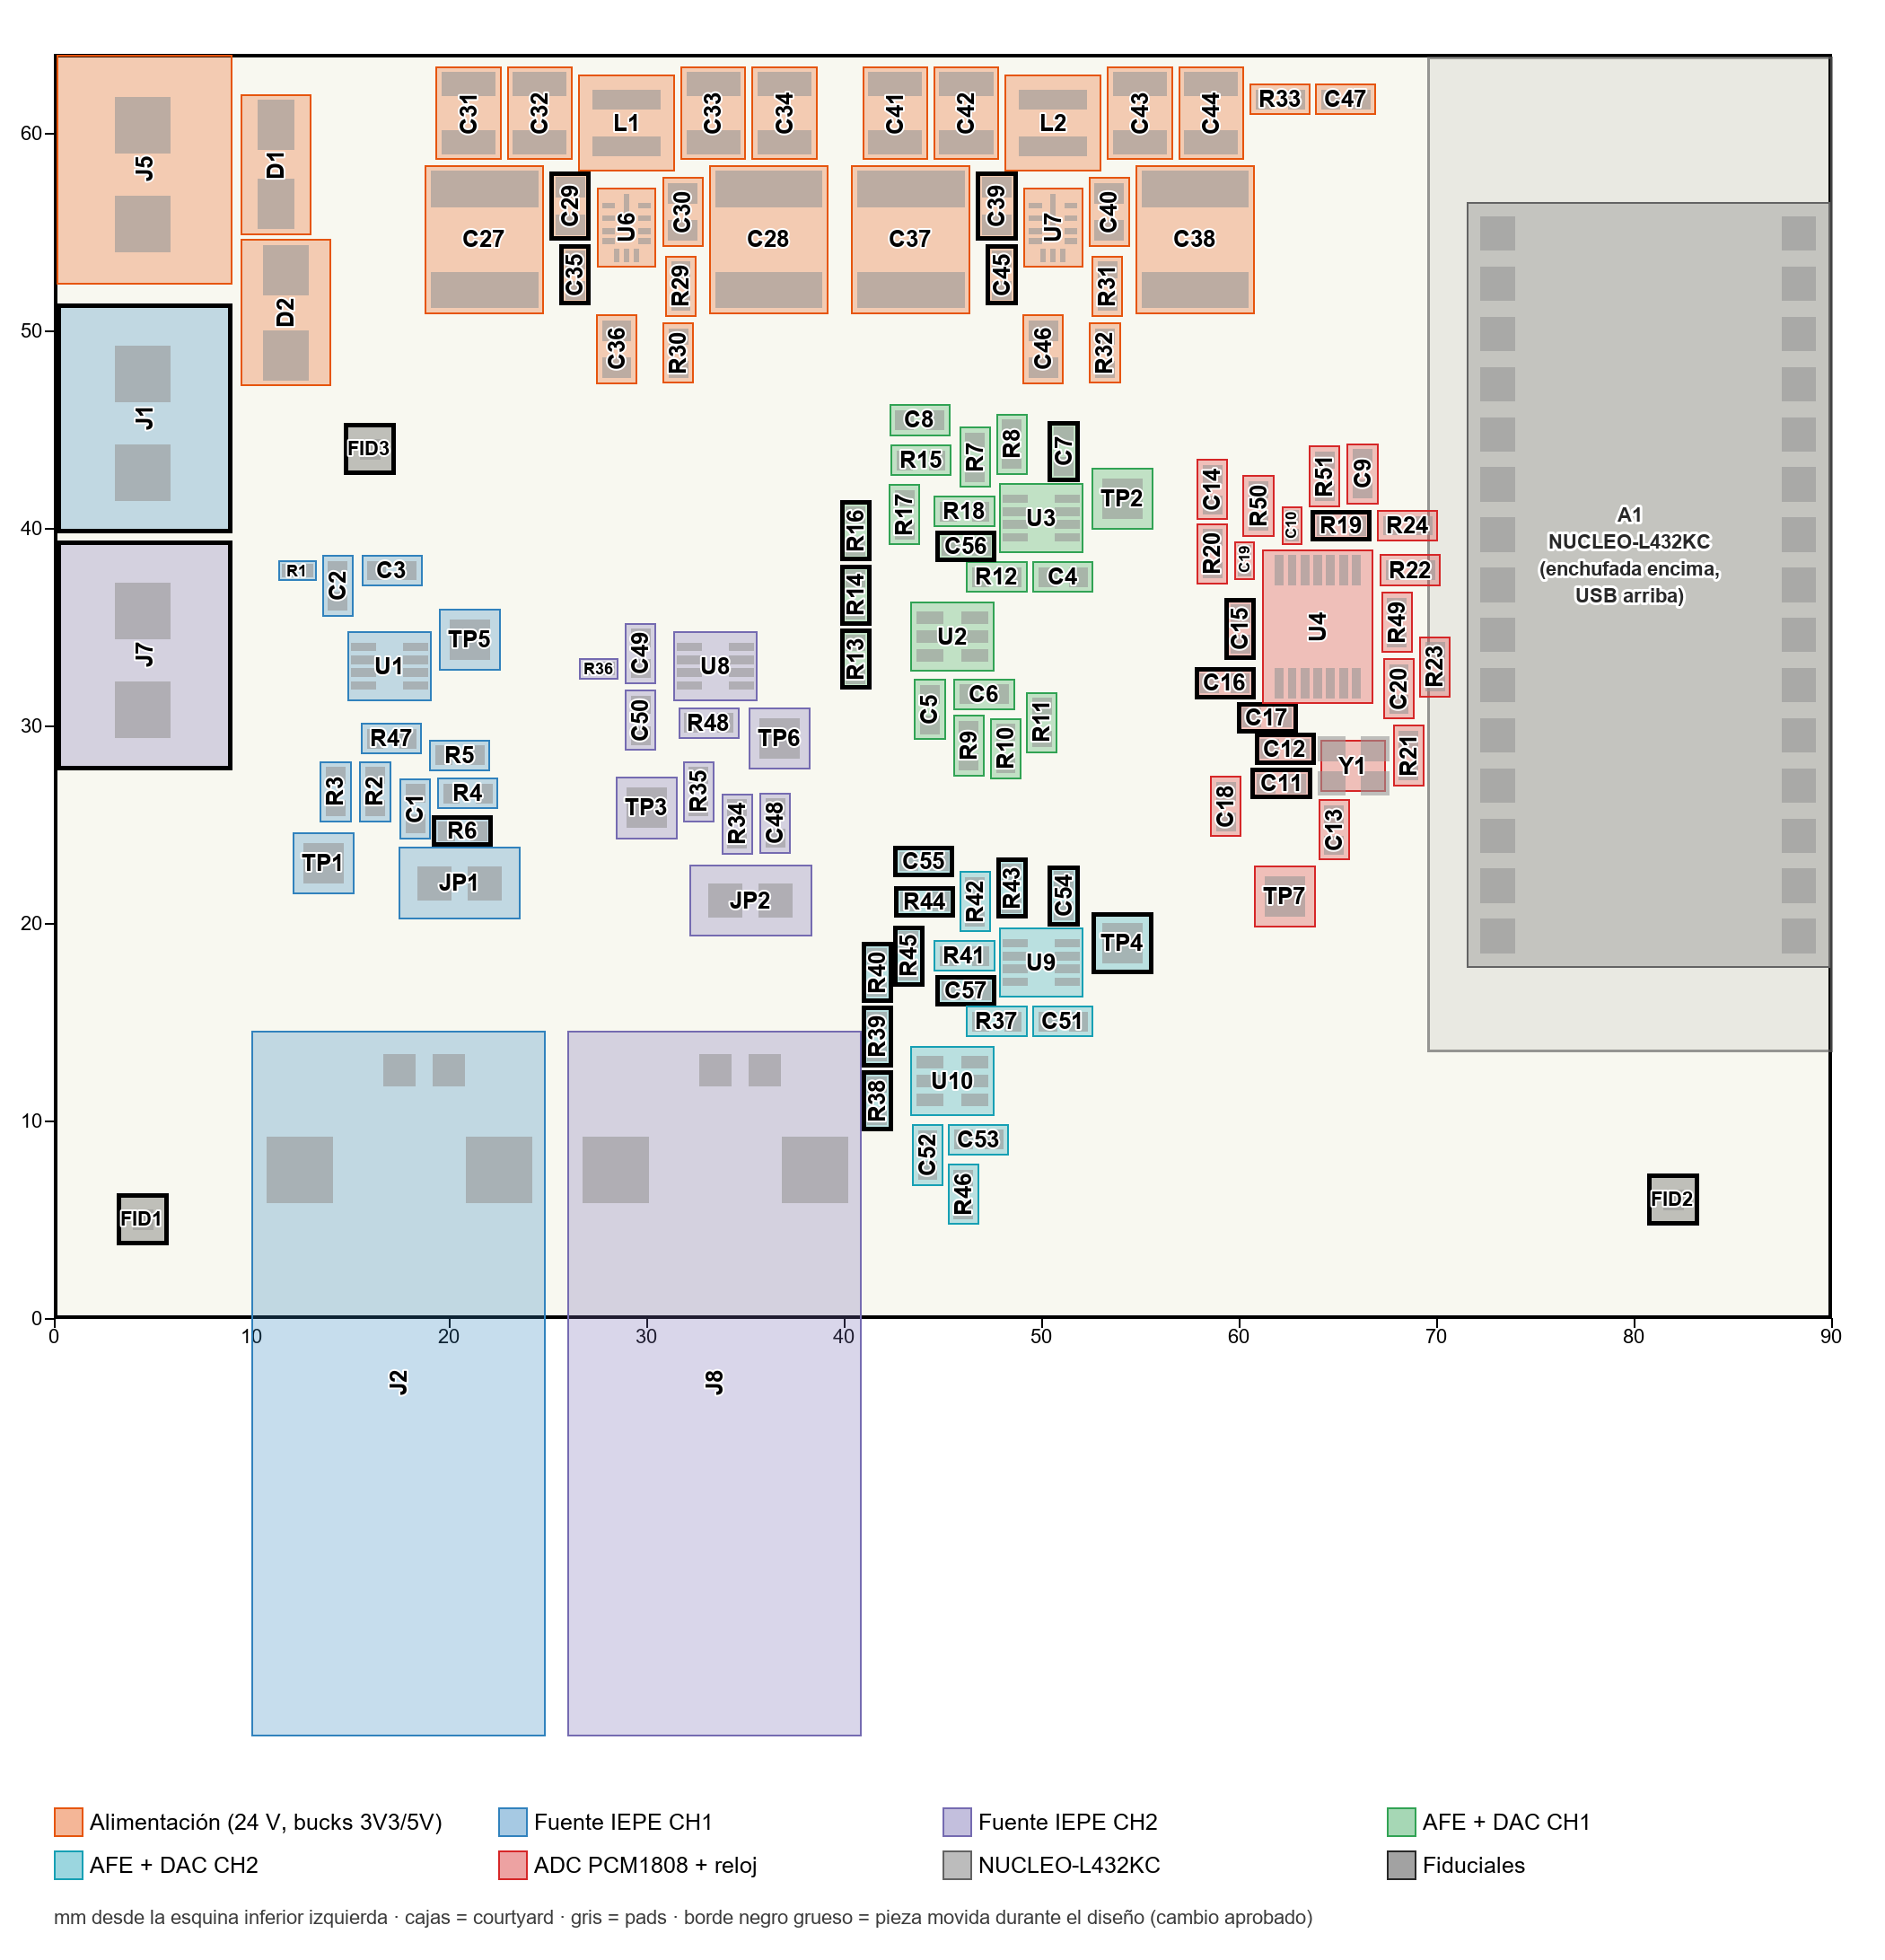
\includegraphics[width=\linewidth]{figuras/c07_mapa_final.png}
\caption{Placement final por bloques, generado a partir de \archivo{pcb.kicad_pcb} (cajas = courtyard, gris =
pads). Los BNC \net{J2} y \net{J8} sobresalen por el borde inferior. Borde negro grueso: pieza movida con un cambio
aprobado.}
\label{fig:c07-mapa}
\end{figure}

Leyendo el mapa de arriba abajo y de izquierda a derecha (posiciones aproximadas, tomadas de la figura):
\begin{itemize}
  \item \textbf{Franja superior, alimentación} ($y \approx 48$ a \SI{64}{\milli\meter}). De izquierda a derecha: la
        bornera de entrada \net{J5}, el diodo serie \net{D1} y el TVS \net{D2}; luego el buck de \SI{3.3}{\volt}
        (\net{U6}, \net{L1}, sus CIN \net{C27}/\net{C28} y sus COUT \net{C31}--\net{C34}) y el de \SI{5}{\volt}
        (\net{U7}, \net{L2}, \net{C37}/\net{C38}, \net{C41}--\net{C44}); al final el filtro \net{R33}/\net{C47} que
        produce \net{5V_A}. Todo lo que conmuta queda en esa franja.
  \item \textbf{Borde izquierdo, conectores}: \net{J5}, \net{J1} y \net{J7}, uno debajo del otro.
  \item \textbf{Centro izquierda, fuentes IEPE}: CH1 (\net{U1} y sus resistencias, $x \approx 12$ a
        \SI{25}{\milli\meter}) y CH2 (\net{U8}, $x \approx 27$ a \SI{40}{\milli\meter}), cada una justo encima de su
        BNC. La corriente sale de la fuente y llega al micrófono por el camino más corto.
  \item \textbf{Centro, los dos AFE}: CH1 arriba ($y \approx 30$ a \SI{47}{\milli\meter}) y CH2 abajo ($y \approx 5$ a
        \SI{25}{\milli\meter}), cada uno con su op-amp (\net{U3}, \net{U9}) y su DAC (\net{U2}, \net{U10}). Las
        columnas de resistencias \net{R13}/\net{R14}/\net{R16} y \net{R38}/\net{R39}/\net{R40} son la cadena de
        \SI{1}{\mega\ohm} de cada canal.
  \item \textbf{Frontera, el ADC} (\net{U4}, $x \approx 58$ a \SI{70}{\milli\meter}): sus entradas miran hacia los AFE
        y su lado digital hacia la NUCLEO. El oscilador \net{Y1} está pegado a él.
  \item \textbf{Borde derecho, zona digital}: la NUCLEO (\net{A1}), de $x \approx 70$ a \SI{90}{\milli\meter}. Por
        debajo de su cuerpo pasan las líneas I2C y DC\_MON hacia sus pines.
\end{itemize}

Para comparar, la figura~\ref{fig:c07-inicial} muestra el placement con el que empezó el ruteo (15 de noviembre).
Ese placement ya estaba verificado (ERC 0, paridad 0, DRC sin errores), pero todavía no tenía ninguna pista: los
problemas solo aparecieron al intentar rutear.

\begin{figure}[!htbp]
\centering
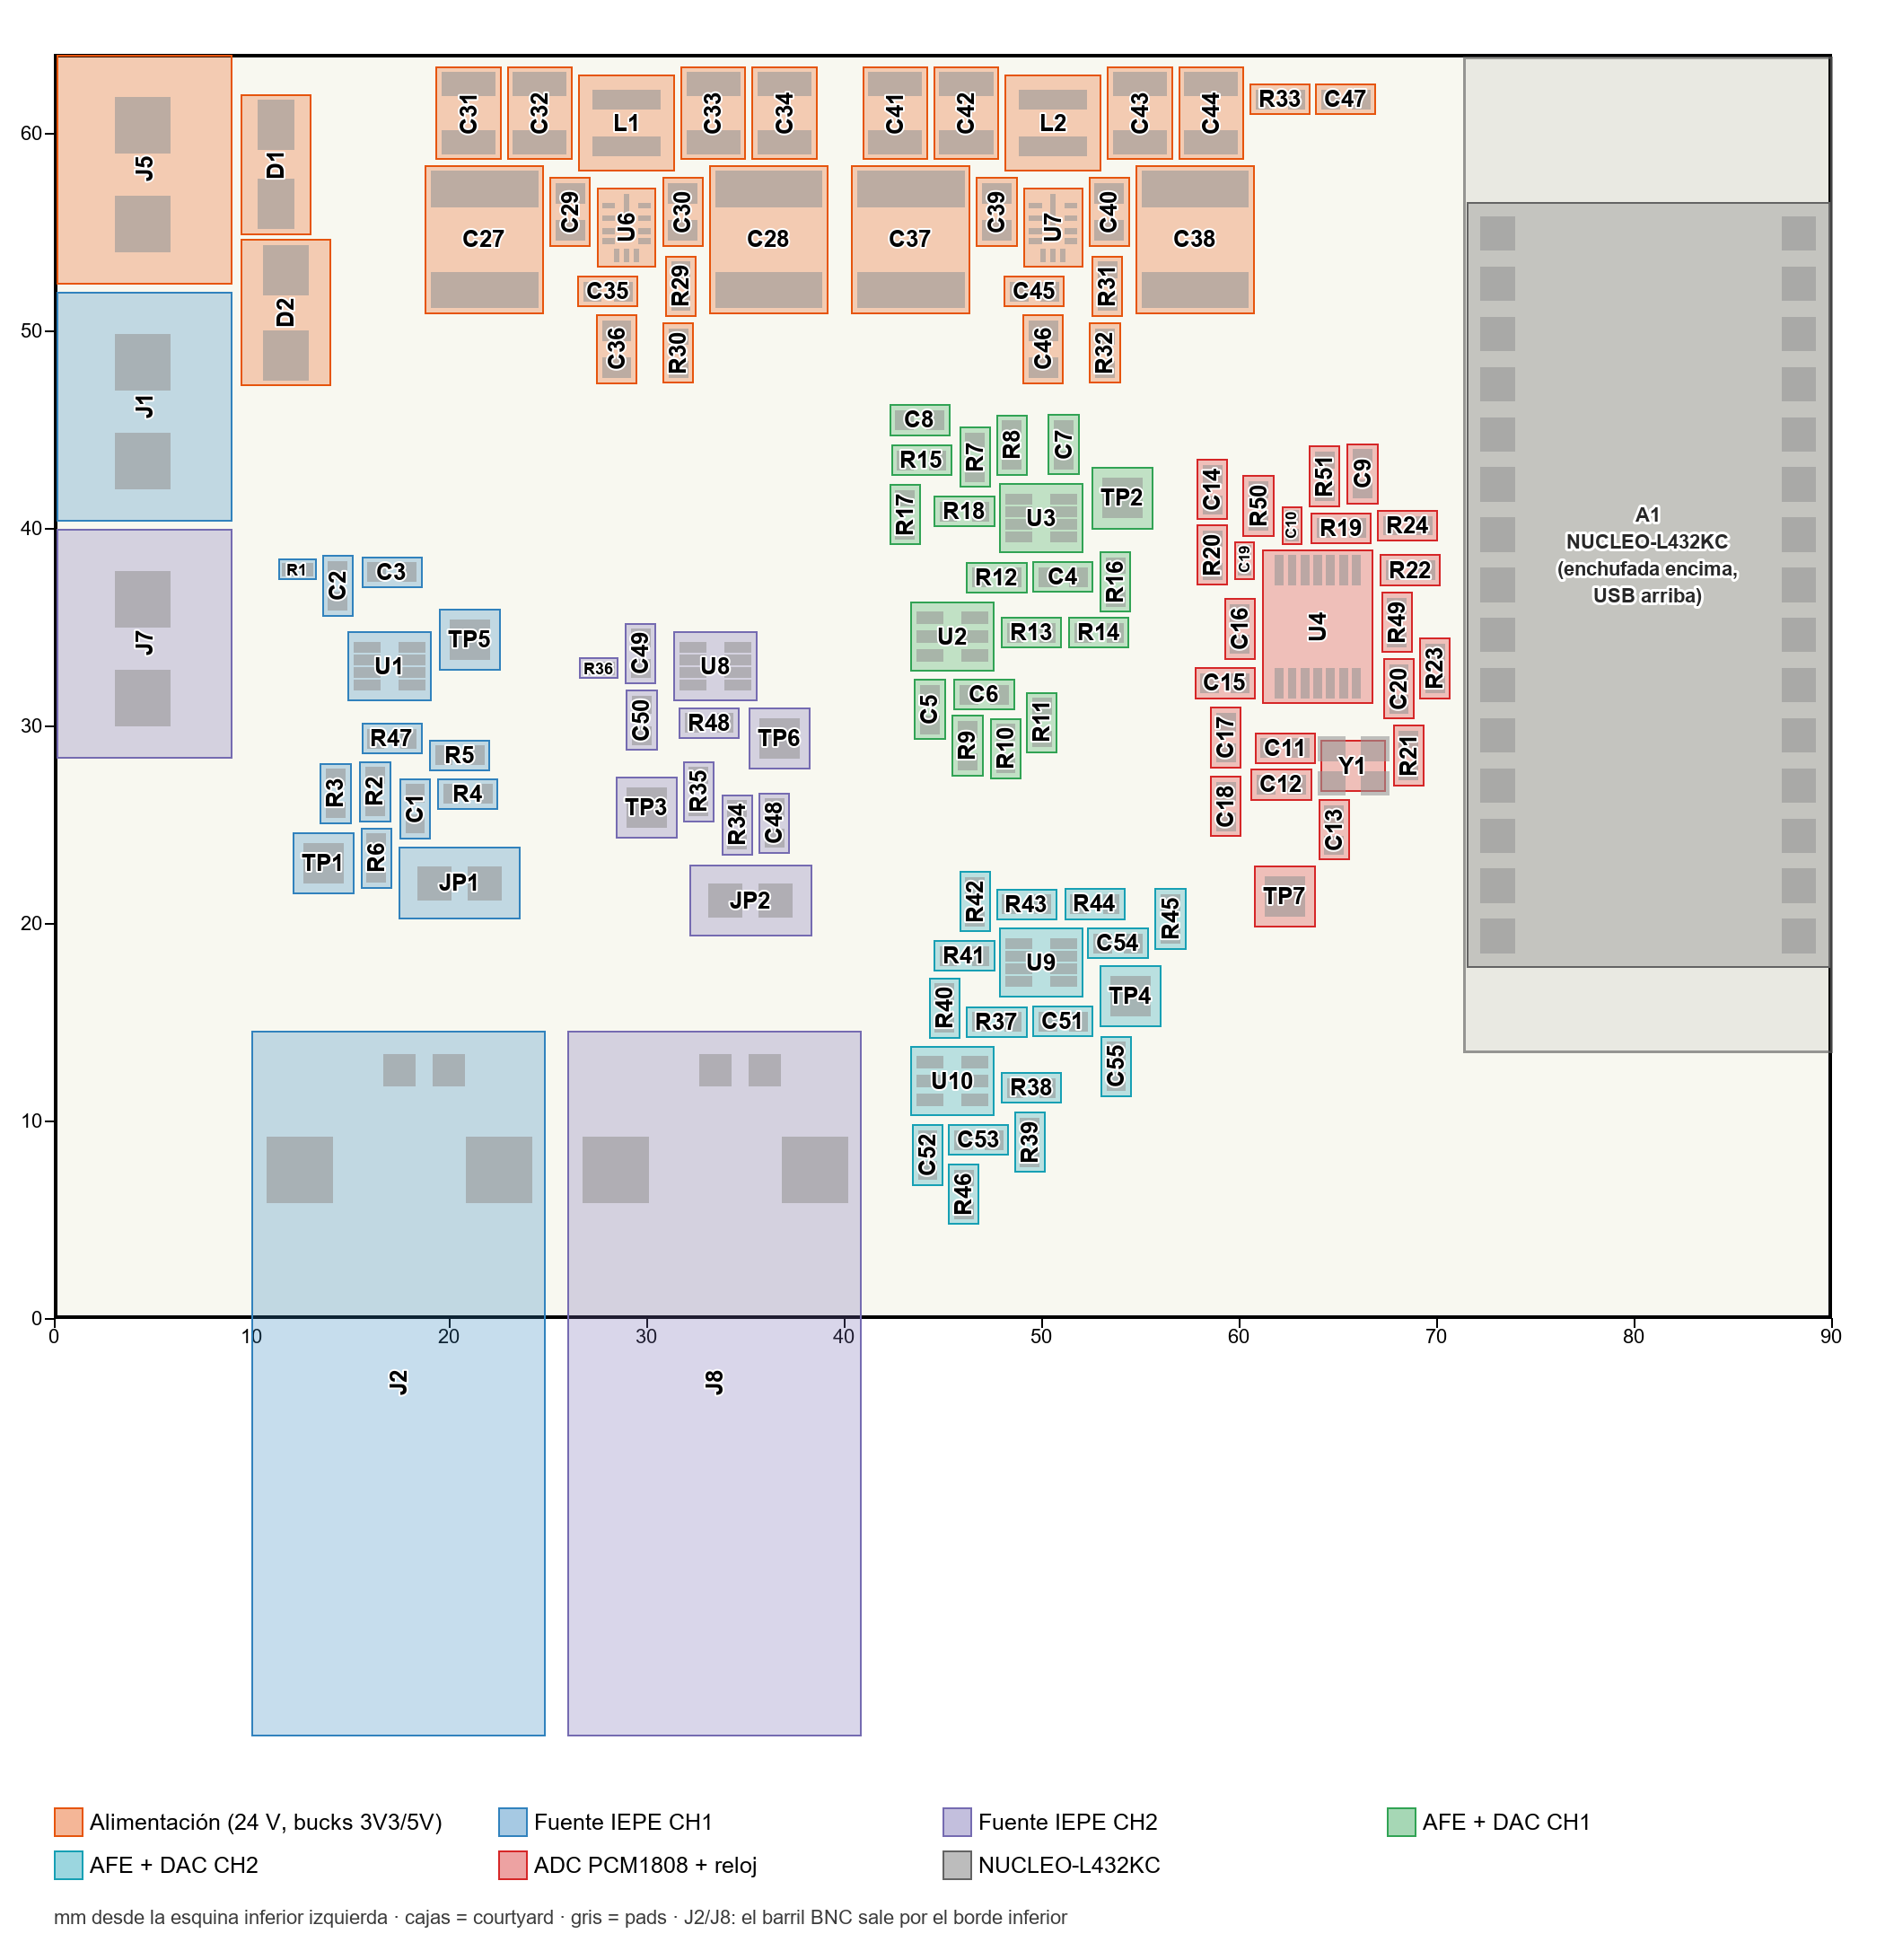
\includegraphics[width=0.66\linewidth]{figuras/placement_map.png}
\caption{Placement inicial de la Rev B, antes de rutear (15/11/2026). Compáralo con la
figura~\ref{fig:c07-mapa}: cambian sobre todo la cadena de \SI{1}{\mega\ohm} de los dos canales, el grupo de
\net{TP4} en CH2 y los desacoplos del ADC.}
\label{fig:c07-inicial}
\end{figure}

% =====================================================================================================
\section{La regla de autorización}\label{sec:c07-autorizacion}

Mover una pieza puede parecer inocente, pero cambia distancias que ya se habían revisado (desacoplos, lazos de
potencia, separaciones). Por eso el dueño del proyecto fijó, el 15/11/2026, dos niveles:

\begin{center}
\begin{tabular}{@{}L{0.46\linewidth}L{0.46\linewidth}@{}}
\toprule
\textbf{Se hace sin preguntar (y se informa al final del bloque)} & \textbf{Se pregunta antes}\\
\midrule
Mover pasivos y puntos de prueba hasta \SI{0.1}{\milli\meter} para alinear pads. &
Mover integrados o conectores.\\
Reubicar textos de serigrafía. & Mover cualquier pieza más de \SI{0.1}{\milli\meter}.\\
Cualquier ajuste que no cambie el esquemático, las piezas ni la topología. &
Cambiar piezas o valores; cualquier excepción a las reglas (DRC, REGLAS.md, chequeo propio).\\
\bottomrule
\end{tabular}
\end{center}

Esta regla está escrita también en el código: la función de alineación de \archivo{tools/eco.py} se niega a mover una
pieza más de \SI{0.1}{\milli\meter} (``supera 0.1 mm (requiere aprobación aparte)''). Los movimientos mayores se
guardan en archivos \archivo{colocar_bloque*.json}, cada uno con el texto de la aprobación, por ejemplo:
\begin{center}
\texttt{"R6": [120.7, 139.35, 180, "aprobado tras el bloque 2: R5.1-R6.1 sin camino\dots"]}
\end{center}

\subsection*{Por qué alinear pads por centésimas de milímetro}
Las reglas de trazado piden quiebres de solo \ang{45}, segmentos de \SI{0.1}{\milli\meter} o más y entrada al pad
por su eje (capítulos~\ref{cap:jlc} y~\ref{cap:ruteo}). Con esas tres reglas, un desfase pequeño entre dos pads
es un problema: si el centro de un pad está \SI{0.05}{\milli\meter} más arriba que el del otro, la pista recta entre
ellos no entra por el eje de ninguno, y para corregirlo harían falta dos quiebres de \ang{45} con un tramo diagonal
de apenas \SI{0.07}{\milli\meter}, más corto que el mínimo (figura~\ref{fig:c07-alinear}). La solución es mover el
pasivo esos \SI{0.05}{\milli\meter} para que los dos pads queden en la misma línea.

\begin{figure}[!htbp]
\centering
\begin{tikzpicture}[x=1cm,y=1cm,font=\small]
  \begin{scope}
    \fill[gray!35] (0,0) rectangle (0.8,0.9);
    \fill[gray!35] (3.2,0.25) rectangle (4.0,1.15);
    \draw[orange!70!brown,line width=2.5pt] (0.4,0.45) -- (1.6,0.45) -- (1.85,0.7) -- (3.6,0.7);
    \draw[red,thick] (1.72,0.57) circle (0.3);
    \node[align=center,font=\footnotesize] at (2.0,-0.55) {pads desalineados: hace falta un quiebre\\con un tramo diagonal muy corto};
  \end{scope}
  \begin{scope}[xshift=6.3cm]
    \fill[gray!35] (0,0.25) rectangle (0.8,1.15);
    \fill[gray!35] (3.2,0.25) rectangle (4.0,1.15);
    \draw[orange!70!brown,line width=2.5pt] (0.4,0.7) -- (3.6,0.7);
    \node[align=center,font=\footnotesize] at (2.0,-0.55) {pad movido unas centésimas:\\pista recta, entra por el eje};
  \end{scope}
\end{tikzpicture}
\caption{Por qué se alinean los pads (dibujo exagerado; el desfase real era de centésimas de milímetro).}
\label{fig:c07-alinear}
\end{figure}

% =====================================================================================================
\section{Los cambios de placement, uno por uno}\label{sec:c07-cambios}

La tabla~\ref{tab:c07-cambios} lista todos los cambios. Después se explican los que tienen más historia.

{\small
\begin{longtable}{@{}L{0.2\linewidth}L{0.3\linewidth}L{0.3\linewidth}L{0.13\linewidth}@{}}
\caption{Cambios de placement aprobados (PLAN\_RUTEO.md y archivos \archivo{colocar_*}/\archivo{alineacion_*}).}
\label{tab:c07-cambios}\\
\toprule
\textbf{Piezas} & \textbf{Cambio} & \textbf{Por qué} & \textbf{Cuándo}\\
\midrule\endfirsthead
\toprule
\textbf{Piezas} & \textbf{Cambio} & \textbf{Por qué} & \textbf{Cuándo}\\
\midrule\endhead
\net{C29}, \net{C39} (CHF) & suben \SI{0.3}{\milli\meter} & lazo VIN--CHF--PGND más corto & punto de control 2\\
\net{C35}, \net{C45} (CBOOT) & a la izquierda del integrado, girados \ang{90} & camino BOOT--SW corto & punto de control 2\\
\net{C56}, \net{C57} & piezas nuevas, junto a \net{U3} y \net{U9} & condensador CF del sumador (capítulo~\ref{cap:analog}) & punto de control 2\\
\net{J1}, \net{J7} & bajan \SI{0.6}{\milli\meter} & que el designador de \net{J5} quepa sin ambigüedad & punto de control 2\\
\net{FID1}--\net{FID3} & fiduciales nuevos & ensamblaje en JLC & punto de control 2\\
32 pasivos y TP & alineación de $\leq$ \SI{0.094}{\milli\meter} & entrada por el eje del pad & bloque 3\\
\net{R6} & a $(\num{120.70}, \num{139.35})$, horizontal, girado \ang{180} & \net{R5.1}--\net{R6.1} sin camino en una capa & bloque 3\\
\net{R13}, \net{R14}, \net{R16} & columna vertical en $x = \num{140.6}$ & la cadena de \SI{1}{\mega\ohm} de CH1 no tenía camino & análisis de los bloques 4--8\\
\net{R19} & sube \SI{0.1}{\milli\meter} & DOUT a $\geq$ \SI{0.5}{\milli\meter} de las entradas analógicas & bloque 4\\
\net{C17}; \net{C11}$\leftrightarrow$\net{C12}; \net{C15}$\leftrightarrow$\net{C16} & \net{C17} junto a \net{U4.3}; los \SI{100}{\nano\farad} pasan al lugar más cercano al pin & desacoplo del PCM1808 & bloque 4\\
\net{C56}; \net{C4}, \net{C6}, \net{R9} & \SI{+0.08}{\milli\meter}; menos de \SI{1}{\micro\meter} & alineación de pads & bloque 5\\
\net{R38}, \net{R39}, \net{R40} & columna en $x = \num{141.7}$ & el nodo R39--R40 encerraba a \net{U10} & bloque 5\\
\net{C57}, \net{R43} & a las posiciones de \net{C56} y \net{R8} de CH1 & SUM, REST\_SV y el nodo R42--R43 se cruzaban & bloque 5\\
\net{TP4}, \net{C54}, \net{R44}, \net{R45}, \net{C55} & a las posiciones de \net{TP2}, \net{C7}, \net{R15}, \net{R17}, \net{C8} de CH1 & \net{REST_SV} quedaba partido & bloque 5\\
\net{C7} & \SI{0.35}{\milli\meter} más abajo & paso para \net{REST_OUT} sin cortar el desacoplo & bloque 5\\
\bottomrule
\end{longtable}
}

Las coordenadas de esta sección son las de KiCad (milímetros, origen arriba a la izquierda, $y$ hacia abajo),
porque así están en los archivos de colocación.

\subsection{Cambios del punto de control 2}
Antes de trazar la primera pista hubo una revisión general (el ``punto de control 2''). Ahí se aprobaron:
\begin{itemize}
  \item \textbf{Bucks.} Los condensadores de \SI{220}{\nano\farad} entre VIN y PGND (\net{C29}, \net{C39}) subieron
        \SI{0.3}{\milli\meter}, y los de BOOT (\net{C35}, \net{C45}) pasaron a la izquierda del integrado, girados
        \ang{90}. El objetivo era el que pide TI: el lazo VIN--CHF--PGND lo más pequeño posible y el condensador de
        BOOT cerca de BOOT y SW \doc{SNVSB49D §12.1}. En el capítulo~\ref{cap:ruteo} están las medidas de esos lazos.
  \item \textbf{CF.} Los condensadores nuevos \net{C56} y \net{C57} se pusieron entre los pines 1 y 2 de cada op-amp,
        que es justo donde se conectan (salida y entrada inversora del sumador).
  \item \textbf{J1 y J7 bajan \SI{0.6}{\milli\meter}.} El designador de \net{J5} es obligatorio (los conectores nunca
        se omiten de la serigrafía) y con las borneras pegadas no había forma de ponerlo sin que se confundiera con
        el de \net{J1}. Se probó en una copia: el DRC no mostró errores nuevos. En la placa, \net{J1} pasó de
        $y = \num{115.6}$ a \num{116.2} y \net{J7} de \num{127.6} a \num{128.2} \medido. Son borneras soldadas a mano.
  \item \textbf{Fiduciales} \net{FID1}--\net{FID3} en $(\num{4.5}, \num{5})$, $(\num{82}, \num{6})$ y
        $(\num{16}, \num{44})$~\si{\milli\meter} desde la esquina inferior izquierda, a \SI{6}{\milli\meter} o más del
        pad más cercano.
\end{itemize}

\subsection{R6: sin camino en una capa}
En el bloque 3 (fuentes IEPE), el enlace \net{R5.1}--\net{R6.1} no tenía camino en una sola capa con \net{R6} en su
lugar original $(\num{116.27}, \num{140.72})$: Freerouting lo dejó sin rutear después de 800 pasadas. Con \net{R6} en
$(\num{120.70}, \num{139.35})$, horizontal y girado \ang{180}, el enlace sale completo. Es una resistencia, pero el
movimiento es de más de \SI{4}{\milli\meter}, así que se pidió aprobación.

\subsection{La columna de la cadena de \SI{1}{\mega\ohm}}
La entrada de cada AFE es una cadena de cuatro resistencias en serie que suma \SI{1}{\mega\ohm}
(\SI{390}{\kilo\ohm} + \SI{365}{\kilo\ohm} + \SI{191}{\kilo\ohm} + \SI{54.9}{\kilo\ohm}). Es un nodo de \emph{alta
impedancia}: cualquier pista que pase cerca le acopla ruido, así que no se le pueden pasar puentes por debajo ni
cruzarlo.

En CH1 había un problema. \net{R14} y \net{R16} estaban a la derecha de \net{U3}, y \net{U3} quedaba ``cerrado'' por
sus propias redes (\net{REST_OUT} hacia \net{R8}, \net{5V_A} hacia \net{C7}, la entrada del seguidor hacia
\net{C4}/\net{R12}, y SUM). El oráculo (sección~\ref{sec:c07-oraculo}) dejaba sin rutear dos enlaces: IEPE hasta
\net{R13.2} y el final de la cadena, \net{R16} hasta \net{R18}.

\begin{decision}[R13, R14 y R16 en columna]
\textbf{Qué se decidió:} poner \net{R13}, \net{R14} y \net{R16} verticales y apiladas en la columna libre
$x = \num{140.6}$ (commit \texttt{0452393}, \archivo{colocar_bloque5.json}).

\textbf{Alternativas:} pasar la cadena por debajo de otras piezas o en otra capa. Ninguna sirve: es un nodo de alta
impedancia.

\textbf{Por qué:} con la columna, IEPE entra a \net{R13} por la izquierda sin meterse al AFE, y la cadena sube y
entra a \net{R18.2} pasando entre los pads de \net{R17}. En la prueba del oráculo, \textbf{todas las redes críticas
de los bloques 4 a 7 salieron en \capa{F.Cu} con 0 vías} (figura~\ref{fig:c07-oraculo}). El DRC no mostró solapes
de courtyard.

\textbf{Fuente:} \archivo{PLAN_RUTEO.md} §10 y §10.1.
\end{decision}

\begin{figure}[!htbp]
\centering
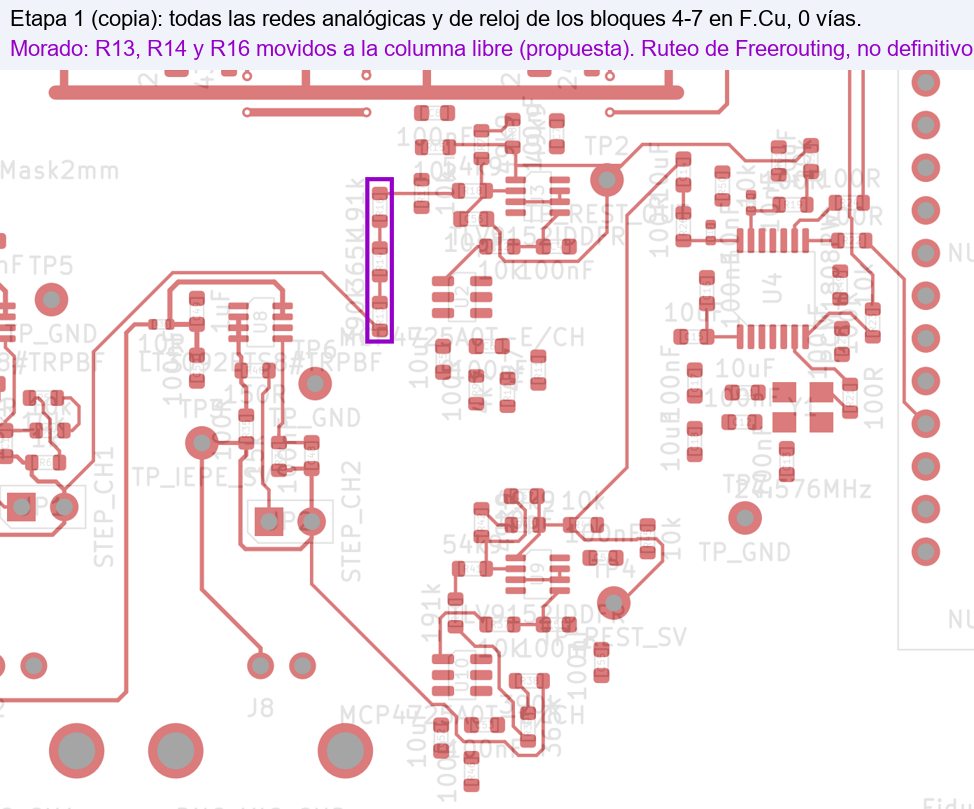
\includegraphics[width=0.78\linewidth]{figuras/oraculo_etapa1_columna.png}
\caption{Prueba del oráculo (en una copia, no es el ruteo final): las redes analógicas y de reloj de los bloques
4--7 en \capa{F.Cu}, sin vías. En morado, \net{R13}, \net{R14} y \net{R16} en la columna libre.}
\label{fig:c07-oraculo}
\end{figure}

\subsection{Los desacoplos del ADC}
Después del bloque 4, el chequeo de desacoplo encontró varios condensadores del PCM1808 lejos de sus pines. Se
aprobó (\archivo{colocar_bloque4.json}):
\begin{itemize}
  \item \net{C17} (\SI{100}{\nano\farad} de \net{5V_A}) junto al pin 3 de \net{U4}, a \SI{0.71}{\milli\meter};
  \item intercambiar \net{C11}$\leftrightarrow$\net{C12} y \net{C15}$\leftrightarrow$\net{C16}, para que el de
        \SI{100}{\nano\farad} quede en el lugar más cercano al pin y el de \SI{10}{\micro\farad} un poco más lejos.
\end{itemize}
Es el criterio 2 de arriba: el condensador pequeño atiende las frecuencias altas y su lazo debe ser el más corto. Aun
así, \net{C12} (\SI{2.12}{\milli\meter}) y \net{C16} (\SI{1.32}{\milli\meter}) quedaron por encima del límite de
\SI{1}{\milli\meter} del chequeo y se aceptaron como excepción (capítulo~\ref{cap:banco}).

También en el bloque 4, \net{R19} subió \SI{0.1}{\milli\meter} (un ajuste autorizado) para que la pista de datos
DOUT pase por debajo de ella a \SI{0.5}{\milli\meter} o más de \net{AC_LEFT}/VINL, que es lo que exige la regla
\net{reloj_lejos_de_analogica}.

\subsection{CH2: hacerlo igual a CH1}
Con la colocación original, CH2 no se podía rutear limpio:
\begin{itemize}
  \item el nodo entre \net{R39} y \net{R40} rodeaba a \net{U10} y encerraba sus salidas SCL (\net{U10.5}) y A0
        (\net{U10.6});
  \item en el grupo de \net{C57}/\net{R43}, las redes SUM, \net{REST_SV} y el nodo R42--R43 se cruzaban: hacían
        falta tres entradas a pads en diagonal, contra la regla de entrar por el eje.
\end{itemize}
Primero se probó la solución en una copia y luego se aprobó en dos pasos:
\begin{enumerate}
  \item \archivo{colocar_bloque5b.json}: \net{R38}, \net{R39} y \net{R40} en columna en $x = \num{141.7}$ (el courtyard
        de \net{J8} llega hasta $x = \num{140.90}$, por eso no se pudo usar $\num{140.6}$ como en CH1); \net{C57} en
        el lugar equivalente al de \net{C56}, $(\num{146.19}, \num{147.43})$; y \net{R43} vertical como \net{R8}.
  \item \archivo{colocar_bloque5c.json}: aun así \net{REST_SV} quedaba partido en dos grupos,
        \{\net{U9.1}, \net{R43.1}, \net{R44.2}\} y \{\net{C57.2}, \net{TP4}\}, porque \net{TP4} estaba encerrado por
        \net{DC_MON2}, \net{C54} y la conexión de \net{5V_A} a \net{U9.8}. Se movieron \net{TP4}, \net{C54},
        \net{R44}, \net{R45} y \net{C55} a los lugares equivalentes de \net{TP2}, \net{C7}, \net{R15}, \net{R17} y
        \net{C8} de CH1 (\net{R44}, \net{R45} y \net{C55} van \SI{0.2}{\milli\meter} más a la derecha, por la
        columna).
\end{enumerate}
El resultado: \textbf{CH2 es CH1 desplazado \SI{22.5}{\milli\meter}}. \net{C57}, \net{R41} y \net{R42} perdieron su
designador en la serigrafía (no cabía) y quedan en el PDF de montaje.

\subsection{C7}
\net{REST_OUT} (la salida del sumador de CH1) tiene que salir de \net{U3.1} hacia la derecha. No cabía entre
\net{U3.8} y su condensador de desacoplo \net{C7} sin cortar el desacoplo. Se bajó \net{C7} \SI{0.35}{\milli\meter}
en total (una alineación de \SI{0.1}{\milli\meter} más \SI{0.25}{\milli\meter} aprobados); queda a
\SI{0.975}{\milli\meter} de \net{U3.8}, todavía dentro del límite de \SI{1}{\milli\meter}, y \net{REST_OUT} pasa por
encima de \net{C7} hacia \net{TP2}.

% =====================================================================================================
\section{Freerouting como oráculo}\label{sec:c07-oraculo}

Freerouting es un \emph{autorouter} libre: le das las piezas y las conexiones y busca pistas que las unan. En este
proyecto \textbf{nunca se usó para el ruteo final}, que se hizo a mano con polilíneas (capítulo~\ref{cap:ruteo}). Se
usó como \emph{oráculo}: en una copia de la placa se le pregunta ``¿existe un camino?'', y su respuesta orienta el
placement. Si un autorouter con cientos de pasadas no encuentra camino para un enlace, es una señal fuerte de que
hay que mover algo.

\begin{ojo}[un oráculo también se equivoca]
La primera prueba de factibilidad con Freerouting tuvo varios problemas, documentados en \archivo{PLAN_RUTEO.md}
§1.2: no se guardó el resultado (así que no se sabía qué conexiones fallaban), usaba los pads viejos del TSOT y
pistas anchas en pines de paso fino (parte de las fallas podían ser de acceso a pines y no cruces), y el límite de
pasadas no se aplicó porque la opción tenía otro nombre. Además, dos procesos quedaron vivos y ocuparon unos
\SI{6}{\giga\byte} de memoria. Por eso sus resultados se tomaron como \emph{indicio}, no como prueba, y las corridas
siguientes se hicieron con memoria limitada, límite de pasadas y guardando el resultado.
\end{ojo}

El análisis de los bloques 4 a 8 se hizo en dos etapas (\archivo{tools/ruteo/oraculo/}):
\begin{enumerate}
  \item \textbf{Redes críticas solas} (analógicas y de reloj, solo en \capa{F.Cu}). Con el placement original
        quedaban sin rutear los dos enlaces de la cadena de CH1. Con la columna, todo salió en \capa{F.Cu} con 0
        vías (figura~\ref{fig:c07-oraculo}).
  \item \textbf{El resto} (alimentación, I2C, DC\_MON, straps) con lo crítico congelado. En 2 capas, o se usaban
        unos \SI{140}{\milli\meter} de \capa{B.Cu} pasando bajo unas 12 redes críticas (y quedaban 3 sin rutear), o
        se penalizaban las vías y quedaban 17 sin rutear. Esta etapa fue la que llevó a la placa de 4 capas
        (capítulo~\ref{cap:capas}).
\end{enumerate}

% =====================================================================================================
\section{Serigrafía y el PDF de montaje}\label{sec:c07-serigrafia}

La serigrafía también es parte del placement: cada designador (``R13'', ``C7'') tiene que caber cerca de su pieza
sin tapar nada. Las reglas, aplicadas por \archivo{tools/ruteo/serigrafia.py}, son:
\begin{itemize}
  \item texto de \SI{1.0}{\milli\meter} de alto y \SI{0.15}{\milli\meter} de trazo (mínimo de JLC), solo a \ang{0} o
        \ang{90} (se lee desde abajo o desde la derecha);
  \item nunca sobre pads (con \SI{0.15}{\milli\meter} de separación), vías, máscara abierta ni sobre el cuerpo de
        ninguna pieza; sin solaparse con otra serigrafía; a \SI{0.5}{\milli\meter} o más del borde;
  \item \textbf{sin ambigüedad}: el texto debe quedar más cerca de su pieza que de cualquier otra del mismo tipo;
  \item si no cabe, el designador se omite. \textbf{Nunca} se omiten las marcas de pin 1 y de polaridad, los
        conectores (\net{J*}, \net{A1}, \net{JP*}) ni los puntos de prueba (\net{TP*}).
\end{itemize}

El script prueba posiciones alrededor de cada pieza (a varias distancias y corrimientos) y se queda con la primera que
cumple todo. El número de omitidos fue cambiando: 28 antes de rutear, 18 con el bloque 1 y \textbf{21 al final}:
\begin{center}
\net{C10} \net{C12} \net{C19} \net{C20} \net{C29} \net{C30} \net{C32} \net{C33} \net{C39} \net{C40} \net{C42}
\net{C43} \net{C57} \net{L1} \net{L2} \net{R7} \net{R18} \net{R19} \net{R22} \net{R41} \net{R42}
\end{center}

Para no perderlos, \archivo{fabricacion/montaje.pdf} dibuja la capa \capa{F.Fab} con \emph{todos} los designadores
dentro del cuerpo de cada pieza (es vectorial: con zoom se leen), y \archivo{fabricacion/LEEME.md} trae una tabla con
la posición de cada omitido.

\begin{ojo}[el orden importa]
Las vías de cosido de tierra (capítulo~\ref{cap:ruteo}) también ocupan lugar. Al principio se ponían antes de la
serigrafía, y entonces varios designadores más se quedaban sin lugar. Se invirtió el orden: primero se coloca la
serigrafía y después \archivo{cosido.py} pone las vías evitando toda la serigrafía. Así se volvió a los mismos 21
omitidos. Además, como
las vías van taponadas, el DRC no ve un texto encima de una vía; para eso se agregó el chequeo M a
\archivo{revisar_pistas.py} (capítulo~\ref{cap:verif}).
\end{ojo}

% =====================================================================================================
\section*{Resumen}
\begin{itemize}
  \item El placement sigue ocho criterios: bloques juntos, desacoplo pegado al pin (el pequeño más cerca), zonas
        analógica y digital sin cortar el plano, ADC en la frontera, oscilador junto a SCKI, conectores al borde, lo
        ruidoso lejos de lo sensible y lo que pide el ensamblaje.
  \item La placa quedó en franjas: alimentación arriba, conectores a la izquierda, fuentes IEPE sobre sus BNC, los
        dos AFE en el centro, el ADC en la frontera y la NUCLEO a la derecha.
  \item Mover más de \SI{0.1}{\milli\meter}, o mover integrados y conectores, necesitó aprobación. Cada movimiento
        aprobado está en un archivo \archivo{colocar_bloque*.json} con su motivo.
  \item Los cambios más importantes fueron la columna de la cadena de \SI{1}{\mega\ohm} en los dos canales y dejar CH2
        idéntico a CH1 desplazado \SI{22.5}{\milli\meter}.
  \item Freerouting se usó solo como oráculo de factibilidad en copias; su segunda etapa mostró que en 2 capas no
        había solución limpia.
  \item 21 designadores no caben en la serigrafía; están en \archivo{fabricacion/montaje.pdf}.
\end{itemize}

\chapter{Por qué la placa terminó en 4 capas}\label{cap:capas}

La placa empezó como un diseño de 2 capas y terminó siendo de 4. No fue un capricho ni una decisión tomada al
principio: salió de intentar rutear con unas reglas concretas y comprobar que con 2 capas no había solución sin romper
esas reglas. Para entender por qué esas reglas importan hay que entender primero una idea que casi nunca se explica
bien en los cursos de circuitos: \textbf{la corriente de retorno}.

\textbf{En este capítulo vas a ver:}
\begin{itemize}
  \item qué es la corriente de retorno y por dónde viaja en una placa;
  \item por qué el área del lazo importa (inductancia, acople y emisiones);
  \item qué pasa cuando el plano de tierra tiene un corte debajo de una pista;
  \item por qué los nodos de alta impedancia del canal analógico son tan delicados;
  \item cuál era la regla de 2 capas, qué cruces la hacían imposible y cómo se comprobó;
  \item qué opciones había, por qué se eligió 4 capas y qué se ganó;
  \item el apilado de JLCPCB, el uso de cada capa y cómo se verifica que se respete;
  \item cuánto cuesta y si sigue sirviendo el ensamblaje económico de JLCPCB.
\end{itemize}

% =====================================================================================================
\section{Toda corriente vuelve}\label{sec:c08-vuelve}

En un esquemático dibujas un cable de la salida de un op-amp a la entrada de otro, y la tierra la pones con un
símbolo. Ese símbolo esconde la mitad del circuito. La corriente que sale por la pista tiene que volver a su fuente,
y vuelve \emph{por la tierra}. Siempre hay un lazo cerrado: ida por la pista, vuelta por la tierra.

\begin{idea}[el lazo siempre existe]
Cada señal de la placa forma una espira: la pista de ida y el camino de vuelta por GND. Esa espira tiene un área.
Todo lo malo que le pasa a una señal en una placa (que capte ruido, que meta ruido en otra, que radie) depende de qué
tan grande es esa área. El trabajo del diseñador de la placa es, en buena parte, \textbf{mantener pequeñas las áreas de
los lazos}.
\end{idea}

\begin{figure}[htbp]
\centering
\begin{circuitikz}
  \fill[cobre!15] (0.6,0.3) rectangle (6.4,2.7);
  \node[cobre!70!black,align=center,font=\small] at (3.5,1.5) {área del lazo\\(lo que hay que minimizar)};
  \draw (0,0) to[sV,l=fuente] (0,3) -- (7,3) to[R,l=carga] (7,0);
  \draw[very thick,red!70!black,-{Latex[length=3mm]}] (1.0,3.35) -- (3.0,3.35);
  \node[right,red!70!black,font=\small] at (3.1,3.35) {pista (ida)};
  \draw[very thick,blue!70!black,-{Latex[length=3mm]}] (6.6,-0.35) -- (4.0,-0.35);
  \node[left,blue!70!black,font=\small] at (3.9,-0.35) {retorno por GND (la mitad que no se dibuja)};
  \draw (0,0) -- (7,0);
\end{circuitikz}
\caption{Una señal es una espira: ida por la pista y vuelta por la tierra. El área encerrada es la que capta y emite
ruido.}
\label{fig:c08-lazo}
\end{figure}

% =====================================================================================================
\section{¿Por dónde vuelve la corriente?}\label{sec:c08-donde}

Supón que la pista sale de un punto A, da una vuelta en L y llega a un punto B, y que debajo hay un plano de tierra
entero (una capa de cobre completa). La corriente de retorno tiene muchos caminos posibles por el plano. ¿Cuál toma?

\begin{itemize}
  \item \textbf{A baja frecuencia (DC y muy poca variación)} la corriente se reparte según la \emph{resistencia}: va más o
  menos en línea recta de B a A, abriéndose por todo el plano, porque ese es el camino de menor resistencia.
  \item \textbf{A alta frecuencia} lo que manda es la \emph{inductancia}, no la resistencia. El camino de menor
  inductancia es el que encierra la menor área con la pista de ida, y ese camino es \textbf{justo debajo de la pista}.
  La corriente de retorno se ``pega'' debajo de la pista y la sigue en su vuelta en L.
\end{itemize}

\begin{figure}[htbp]
\centering
\begin{tikzpicture}[scale=0.85]
  % (a) baja frecuencia
  \begin{scope}
    \fill[verdeplaca!12] (0,0) rectangle (6,4);
    \node[above] at (3,4) {\small (a) baja frecuencia: menor resistencia};
    \draw[line width=2.2pt,cobre] (0.8,0.8) -- (5.2,0.8) -- (5.2,3.2);
    \filldraw[fill=white,draw=black] (0.8,0.8) circle (0.12) node[below left]{A};
    \filldraw[fill=white,draw=black] (5.2,3.2) circle (0.12) node[above right]{B};
    \foreach \d in {-0.5,-0.25,0,0.25,0.5}{
      \draw[blue!70!black,-{Latex[length=2mm]},densely dashed] ($(5.2,3.2)+(\d,\d*-0.9)$) .. controls ($(3,2)+(\d*1.6,\d*-1.6)$) .. ($(0.8,0.8)+(\d*0.5,\d*-0.4)$);
    }
    \node[blue!70!black,font=\small,align=center] at (2.2,2.9) {retorno\\repartido};
  \end{scope}
  % (b) alta frecuencia
  \begin{scope}[xshift=7.2cm]
    \fill[verdeplaca!12] (0,0) rectangle (6,4);
    \node[above] at (3,4) {\small (b) alta frecuencia: menor inductancia};
    \draw[line width=9pt,blue!25] (0.8,0.8) -- (5.2,0.8) -- (5.2,3.2);
    \draw[line width=2.2pt,cobre] (0.8,0.8) -- (5.2,0.8) -- (5.2,3.2);
    \draw[blue!70!black,-{Latex[length=2mm]},thick] (5.55,3.0) -- (5.55,1.2);
    \draw[blue!70!black,-{Latex[length=2mm]},thick] (5.0,0.45) -- (1.2,0.45);
    \filldraw[fill=white,draw=black] (0.8,0.8) circle (0.12) node[above left]{A};
    \filldraw[fill=white,draw=black] (5.2,3.2) circle (0.12) node[above right]{B};
    \node[blue!70!black,font=\small,align=center] at (2.6,2.3) {el retorno va\\debajo de la pista};
  \end{scope}
\end{tikzpicture}
\caption{Vista desde arriba de una pista (cobre) sobre un plano de tierra entero (verde). A baja frecuencia el retorno
(azul) toma el camino de menor resistencia; a alta frecuencia se concentra debajo de la pista, que es el lazo de menor
área.}
\label{fig:c08-retorno}
\end{figure}

¿Qué es ``alta frecuencia'' en esta placa? Hay que pensar en los \emph{flancos}, no solo en la frecuencia de repetición.
El nodo de conmutación de los buck (\net{SW_3}, \net{SW_5}) cambia de \SI{0}{\volt} a \SI{24}{\volt} un millón de
veces por segundo, en unos pocos nanosegundos. El reloj de \SI{24.576}{\mega\hertz} del ADC y las líneas I2S
(\net{SAI_SCK}, \net{SAI_FS}, \net{SAI_SD}) también tienen flancos de nanosegundos. Esos flancos tienen contenido
espectral de decenas a cientos de \si{\mega\hertz}, y ahí la corriente de retorno se comporta como en la
figura~\ref{fig:c08-retorno}(b). Hasta el audio, que es lento, se beneficia: la pista de una señal analógica sobre un
plano entero forma un lazo diminuto que casi no capta campo magnético de los vecinos.

\begin{figure}[htbp]
\centering
\begin{tikzpicture}[scale=1.0]
  \fill[green!20!black!8] (0,0) rectangle (9,0.9);
  \node[font=\small] at (7.4,0.45) {prepreg 7628, $\approx$\SI{0.21}{\milli\meter}};
  \fill[verdeplaca!70] (0,-0.12) rectangle (9,0);
  \node[font=\small,anchor=west,text=verdeplaca] at (9.1,-0.06) {\capa{In1.Cu} = GND};
  \fill[cobre] (3.6,0.9) rectangle (4.6,1.07);
  \node[font=\small,anchor=south] at (4.1,1.1) {pista en \capa{F.Cu}};
  \foreach \a in {0.35,0.7,1.1,1.6}{
    \draw[gray,thin] (4.1-\a*0.35,0.9) .. controls (4.1-\a*0.9,0.6) and (4.1-\a*1.3,0.2) .. (4.1-\a*1.4,0);
    \draw[gray,thin] (4.1+\a*0.35,0.9) .. controls (4.1+\a*0.9,0.6) and (4.1+\a*1.3,0.2) .. (4.1+\a*1.4,0);
  }
  \draw[thick] (4.1,0.985) circle (0.07); \fill (4.1,0.985) circle (0.02);
  \foreach \x/\s in {3.5/0.6,3.85/1,4.1/1.3,4.35/1,4.7/0.6}{
    \draw[blue!70!black,line width=\s pt] (\x-0.05,-0.11) -- (\x+0.05,-0.01) (\x-0.05,-0.01) -- (\x+0.05,-0.11);
  }
  \node[font=\small,blue!70!black,anchor=north] at (4.1,-0.2) {retorno concentrado debajo (más denso al centro)};
\end{tikzpicture}
\caption{Corte transversal: la pista de \capa{F.Cu} queda a unos \SI{0.21}{\milli\meter} del plano \capa{In1.Cu}.
El campo (gris) se cierra sobre el plano y la corriente de retorno (cruces azules, entrando a la hoja) se concentra
justo debajo de la pista, que lleva la corriente de ida (punto, saliendo de la hoja).}
\label{fig:c08-corte}
\end{figure}

% =====================================================================================================
\section{Área del lazo: inductancia, acople y emisiones}\label{sec:c08-area}

Un lazo de corriente es, literalmente, una espira. De electromagnetismo recuerdas tres cosas que aplican aquí:

\begin{enumerate}
  \item \textbf{Inductancia.} La inductancia de una espira crece con su área. Si la corriente cambia rápido, aparece
  una tensión $v = L\,\dfrac{di}{dt}$ que no estaba en el esquemático: picos y oscilaciones.
  \item \textbf{Acople (diafonía).} Dos espiras cercanas comparten flujo magnético (inductancia mutua $M$). Lo que pasa
  en una induce $v = M\,\dfrac{di}{dt}$ en la otra. Menos área = menos flujo compartido.
  \item \textbf{Emisiones y susceptibilidad.} Una espira grande es una antena: radia cuando por ella pasa corriente
  rápida y capta campos externos (por ejemplo los \SI{60}{\hertz} de la red o el propio buck).
\end{enumerate}

\begin{calculo}[orden de magnitud del pico en el lazo del buck]
El lazo de entrada del buck (condensador de entrada, pin \net{VIN}, pin \net{PGND}) conmuta la corriente de la bobina
en cada flanco. En el peor caso esa corriente llega a unos \SI{275}{\milli\ampere} \medido{} (pico en
\net{SW_3}/\net{SW_5}, tabla de anchos de \archivo{CALCULOS.md}). Si el flanco dura unos \SI{10}{\nano\second}
\estimado{} (el mismo supuesto de \archivo{CALCULOS.md}):
\[
\frac{di}{dt} \approx \frac{\SI{0.275}{\ampere}}{\SI{10}{\nano\second}} = \SI{27.5}{\mega\ampere\per\second}.
\]
Con apenas \SI{1}{\nano\henry} de inductancia parásita en el lazo \estimado{}:
\[
v = L\,\frac{di}{dt} = \SI{1}{\nano\henry}\times\SI{27.5}{\mega\ampere\per\second} \approx \SI{28}{\milli\volt}
\]
en cada flanco, un millón de veces por segundo. Si el lazo fuera diez veces más grande, el pico sería unas diez veces
mayor. Por eso el lazo VIN--CHF--PGND del buck se dibujó lo más chico posible (capítulo~\ref{cap:ruteo}): mide
\SI{7.25}{\milli\meter} de perímetro y \SI{3.32}{\milli\meter\squared} de área en un lado del integrado
\medido{}.
\end{calculo}

% =====================================================================================================
\section{Qué pasa si el plano tiene un corte}\label{sec:c08-ranura}

Ahora imagina que debajo de la pista el plano tiene un corte (una ranura). Puede ser porque otra pista pasa por esa
capa, porque hay una fila de vías con sus holguras unidas, o porque alguien partió el plano en ``tierra analógica'' y
``tierra digital''. La corriente de retorno de alta frecuencia quería ir justo debajo de la pista, pero ahí no hay
cobre: tiene que \textbf{rodear la ranura}.

\begin{figure}[htbp]
\centering
\begin{tikzpicture}[scale=0.95]
  \fill[verdeplaca!12] (0,0) rectangle (10,4);
  \fill[white] (4.4,0.9) rectangle (5.6,4);
  \draw[gray] (4.4,0.9) rectangle (5.6,4);
  \node[font=\small,gray!50!black,anchor=south] at (5,4.05) {ranura en el plano};
  \fill[rojoojo!20] (4.2,2) rectangle (5.8,0.6);
  \draw[line width=2.4pt,cobre] (1,2) -- (9,2);
  \node[above,font=\small] at (2.6,2.05) {pista (ida)};
  \draw[blue!70!black,thick,-{Latex[length=2.2mm]}] (9,1.8) -- (5.8,1.8) -- (5.8,0.6) -- (4.2,0.6) -- (4.2,1.8) -- (1.2,1.8);
  \node[font=\small,blue!70!black,align=left,anchor=west] at (6.0,1.05) {el retorno tiene\\que rodear la ranura};
  \node[font=\small,rojoojo,anchor=north] at (5,0.5) {área extra del lazo};
  \filldraw[fill=white] (1,2) circle (0.1); \filldraw[fill=white] (9,2) circle (0.1);
\end{tikzpicture}
\caption{Una ranura en el plano obliga a la corriente de retorno a rodearla. El lazo crece (rojo): más inductancia,
más acople y la ranura misma se comporta como una antena.}
\label{fig:c08-ranura}
\end{figure}

Las consecuencias son las de la sección anterior, pero peores: el lazo crece justo donde está la ranura, y la ranura
pone en el mismo camino de retorno a todas las señales que la cruzan, así que se acoplan entre ellas. Por eso la nota
de TI SLYT499 pide \textbf{un solo plano de tierra, sin cortes ni ranuras bajo las pistas}, y advierte que hasta las
holguras de las vías pueden formar ranuras si se alinean \doc{SLYT499 p.8}. Y la nota SLYT512 explica cómo ordenar una
placa con convertidor: un solo plano, \emph{repartido por zonas} (lo analógico se rutea sobre su zona y lo digital
sobre la suya) en lugar de partido \doc{SLYT512 pp.5--6}.

\begin{ojo}[una pista en el plano también es una ranura]
En una placa de 2 capas en la que \capa{B.Cu} hace de plano, \textbf{cada pista que pongas en \capa{B.Cu} corta el
plano}. El relleno de tierra se aparta de la pista dejando una franja sin cobre: eso es una ranura. Si encima de esa
franja pasa una señal sensible en \capa{F.Cu}, su retorno tiene que rodear. Esta es la raíz de todo el problema de las
2 capas.
\end{ojo}

% =====================================================================================================
\section{Por qué los nodos de alta impedancia son delicados}\label{sec:c08-altaz}

El canal analógico tiene nodos de impedancia muy alta: la cadena de \SI{1}{\mega\ohm} que baja la señal del micrófono
(\net{R13}, \net{R14}, \net{R16}, \net{R18}, capítulo~\ref{cap:analog}), el nodo filtrado del DAC (\net{DAC_F}) y el
nodo medio de la realimentación (\net{FB_MID}). En esos nodos un acople capacitivo pequeño basta para meter ruido.

\begin{calculo}[acople capacitivo en un nodo de la cadena de 1 M$\Omega$]
Toma el nodo \net{IEPE_DIV1}, entre \net{R13} (\SI{390}{\kilo\ohm}) y \net{R14} (\SI{365}{\kilo\ohm}). Hacia
la derecha la cadena sigue con \SI{191}{\kilo\ohm} y \SI{54.9}{\kilo\ohm} hasta el nodo \net{SUM}, que es una tierra
virtual del op-amp, y hacia la izquierda está la salida del micrófono, de baja impedancia. La impedancia que ``ve''
ese nodo es el paralelo:
\[
R_\text{th} = \SI{390}{\kilo\ohm} \parallel (\num{365}+\num{191}+\num{54.9})\,\si{\kilo\ohm}
= \SI{390}{\kilo\ohm} \parallel \SI{610.9}{\kilo\ohm} \approx \SI{238}{\kilo\ohm}.
\]
Supón que una pista ruidosa pasa cerca y forma con el nodo una capacidad parásita de solo \SI{0.1}{\pico\farad}
\estimado{}. Para la componente de \SI{1}{\mega\hertz} del buck:
\[
X_C = \frac{1}{2\pi f C} = \frac{1}{2\pi\cdot\SI{1}{\mega\hertz}\cdot\SI{0.1}{\pico\farad}} \approx \SI{1.59}{\mega\ohm}.
\]
El acople es un divisor entre $X_C$ y $R_\text{th}$:
\[
\frac{|v_\text{nodo}|}{|v_\text{ruido}|} = \frac{R_\text{th}}{\sqrt{R_\text{th}^2 + X_C^2}}
= \frac{238}{\sqrt{238^2+1590^2}} \approx \num{0.15}.
\]
¡Un 15\,\% del ruido pasa al nodo! Si el mismo acople fuera sobre un nodo de \SI{50}{\ohm} (la salida de un op-amp o
de un micrófono IEPE), la relación sería $50/1.59\times10^{6} \approx \num{3e-5}$. Por eso la regla es estricta con
estos nodos: nada ruidoso cerca, y nada que pase por debajo en otra capa.
\end{calculo}

% =====================================================================================================
\section{La regla original para 2 capas}\label{sec:c08-regla2}

Con todo lo anterior, esta fue la regla de ruteo que se aprobó al principio para una placa de 2 capas (punto de
control 2, sección 1 de \archivo{PLAN_RUTEO.md}):

\begin{itemize}
  \item \capa{B.Cu} es el plano de tierra, lo más entero posible.
  \item Las señales críticas (relojes, nodos \net{SW}, \net{IEPE}, \net{SUM}, la cadena de \SI{1}{\mega\ohm},
  \net{REST}, entradas del ADC, \net{VREF}, salidas filtradas de los DAC) van \textbf{100\,\% en \capa{F.Cu}} y
  \textbf{nunca encima de una pista de \capa{B.Cu}}.
  \item Solo I2C, \net{DC_MON} y \net{DC_MON2} (señales lentas o de DC) pueden bajar a \capa{B.Cu}, en puentes
  cortos (\SI{5}{\milli\meter} o menos), con vías de cosido en los extremos y \textbf{solo en la zona digital} (del
  lado de la NUCLEO, $x \geq \SI{70}{\milli\meter}$).
  \item Los cruces que quedaran se resolvían por topología o pasando por debajo de una resistencia o condensador 0603
  en la misma capa (entre los dos pads de un 0603 quedan \SI{0.85}{\milli\meter} libres, y cabe una pista de
  \SI{0.2}{\milli\meter} con su separación).
\end{itemize}

Más adelante se aprobaron tres puentes cortos en \capa{B.Cu} debajo del bus de \SI{24}{\volt} (el tronco de
\net{3V3} y los sensados de realimentación de los dos buck), porque ahí solo se cruzan redes de potencia entre sí.

% =====================================================================================================
\section{Por qué no tenía solución}\label{sec:c08-sinsolucion}

\subsection{Los cruces inevitables}

Un cruce es inevitable cuando dos redes tienen que conectar puntos que quedan ``del otro lado'' de la otra. Piénsalo
como dos caminos en un mapa: si la red A tiene que unir dos puntos y la red B, junto con las piezas que conecta, forma
una barrera cerrada entre ellos, A no puede llegar sin cruzar B. En una sola capa eso no tiene arreglo; o pasas por
debajo de una pieza (si la red B tiene una pieza en serie con espacio entre pads), o cambias de capa.

\begin{figure}[htbp]
\centering
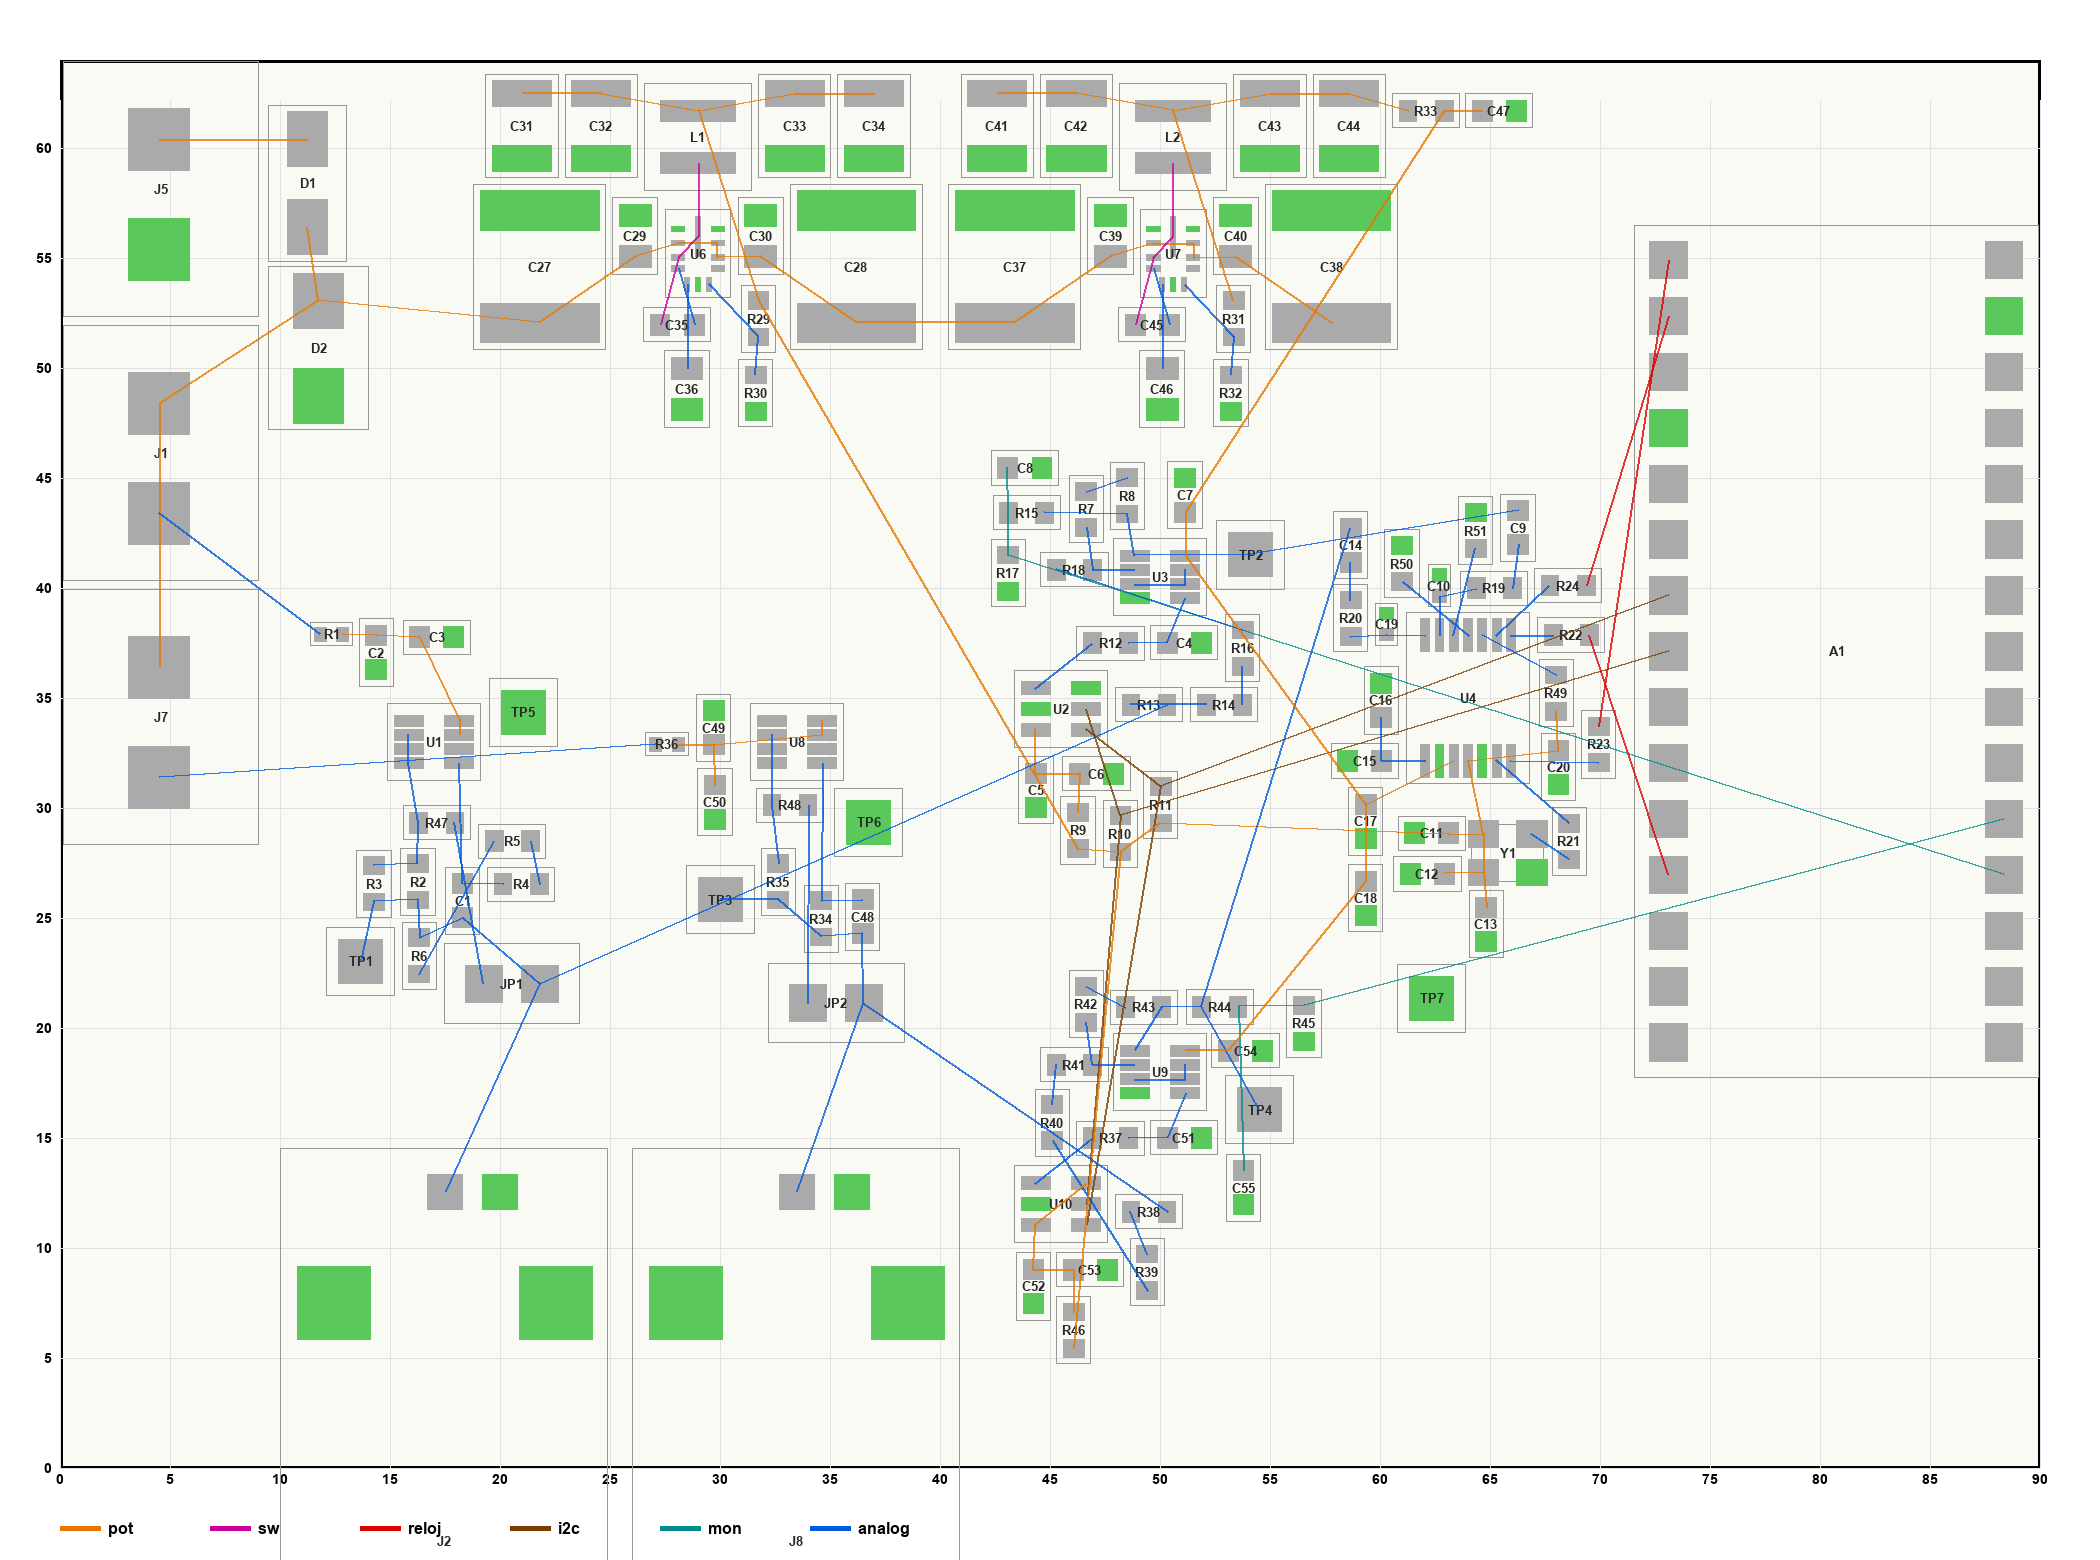
\includegraphics[width=\linewidth]{figuras/c08_ratsnest.png}
\caption{Mapa de las conexiones pendientes antes de rutear (``ratsnest'') sobre el placement, sin GND. Coordenadas en
mm desde la esquina inferior izquierda. Colores: potencia (naranja), nodos SW (magenta), reloj (rojo), I2C (marrón),
\net{DC_MON} (verde azulado) y analógicas (azul). Fíjate en las líneas marrones del I2C y las verde azuladas de
\net{DC_MON}: nacen en los AFE, al centro, y tienen que llegar a la NUCLEO (\net{A1}), a la derecha, atravesando el ADC y
las líneas azules que bajan.}
\label{fig:c08-ratsnest}
\end{figure}

Con el placement real, el análisis a mano encontró estos cruces (\archivo{PLAN_RUTEO.md}~§1.1):

\begin{center}
\begin{tabularx}{\linewidth}{@{}L{0.21\linewidth}Y@{}}
\toprule
\textbf{Cruce} & \textbf{Por qué no se evita en una capa} \\
\midrule
\net{3V3} × \net{24V_PROT} & El buck de \SI{3.3}{\volt} (\net{U6}) queda encerrado por la entrada
(\net{J5}--\net{D1}--\net{D2}), los condensadores de entrada, el bus de \SI{24}{\volt} hacia \net{U7} y el borde
superior. El bus de \SI{24}{\volt} no tiene una pieza en serie bajo la que pasar. \\
\net{5V_A} × \net{REST_OUT} & \net{5V_A} llega a \net{U3} (pin 8, condensador \net{C7}) por la derecha y
\net{REST_OUT} sale de \net{U3} (pin 1) también hacia la derecha: tiene que cruzar el enlace \net{C7}--\net{U3.8}. \\
\net{5V_A} × \net{REST_SV} & \net{REST_SV} sube de \net{U9} a \net{C14} entre el AFE y el ADC; \net{5V_A} tiene que
llegar a \net{U9} y \net{U3}, que quedan del otro lado. \\
I2C × redes del AFE & Los DAC \net{U2} y \net{U10} están dentro de los AFE, rodeados por \net{REST}, la cadena de
\SI{1}{\mega\ohm} y \net{5V_A}. \\
\bottomrule
\end{tabularx}
\end{center}

\subsection{El ``oráculo'': usar un autorouter para preguntar si hay solución}

Para no depender solo de razonamientos a mano, se usó Freerouting (un autorouter libre) sobre \emph{copias} de la
placa, como herramienta de factibilidad. La idea: si un autorouter, que prueba miles de caminos, no encuentra solución
con una regla, es una señal fuerte de que no la hay. A eso se le llamó el \textbf{oráculo}. Lo que sale del oráculo
\emph{nunca} se copió a la placa: el ruteo real se hizo a mano (capítulo~\ref{cap:ruteo}).

\begin{ojo}[un primer intento que no probaba nada]
La primera corrida de Freerouting bajó de 74 a 32--36 conexiones sin rutear y se estancó. Ese número se trató como
\textbf{indicio, no prueba}: no se guardó el resultado, usaba los pads viejos del TSOT, anchos de \SI{0.5}{\milli\meter}
en pines de paso \SIrange{0.5}{0.65}{\milli\meter} (fallas que podían ser de acceso a pines y no de cruces), no hubo
corrida de control y el límite de pasadas estaba mal configurado. Se rehízo bien, por etapas, en copias.
\end{ojo}

\textbf{Etapa 1, solo las redes críticas} (analógicas y relojes de los bloques 4--7, todo en \capa{F.Cu}). Con el
placement original quedaba sin rutear el AFE del canal 1 en dos enlaces (\net{IEPE}~$\to$~\net{R13.2} y el final de
la cadena, \net{R16}~$\to$~\net{R18}): \net{U3} quedaba encerrado por sus propias redes. Se propuso poner
\net{R13}, \net{R14} y \net{R16} en una columna vertical libre ($x = \num{140.6}$ en coordenadas de KiCad) y con eso \textbf{todas las redes críticas
salieron en \capa{F.Cu} sin una sola vía}. Ese cambio de placement se aprobó (capítulo~\ref{cap:placement}).

\textbf{Etapa 2, el resto} (alimentación, I2C, \net{DC_MON}, straps), con las críticas ya fijas:

\begin{center}
\begin{tabularx}{\linewidth}{@{}L{0.27\linewidth}YL{0.16\linewidth}@{}}
\toprule
\textbf{Corrida} & \textbf{Uso de \capa{B.Cu}} & \textbf{Sin rutear} \\
\midrule
\capa{B.Cu} libre para esas redes & unos \SI{140}{\milli\meter} en 7 tramos, debajo de unas 12 redes críticas
(\net{REST_SV}, \net{SAI_FS}, \net{SAI_SCK}, \net{DOUT}, \net{VINL}, \net{AC_RIGHT}, \net{VSHIFT}, \net{REST_OUT}…) & 3 \\
Vías penalizadas & I2C casi entero en \capa{B.Cu}, unos \SI{37}{\milli\meter} por línea & 17 \\
\bottomrule
\end{tabularx}
\end{center}

\begin{figure}[htbp]
\centering
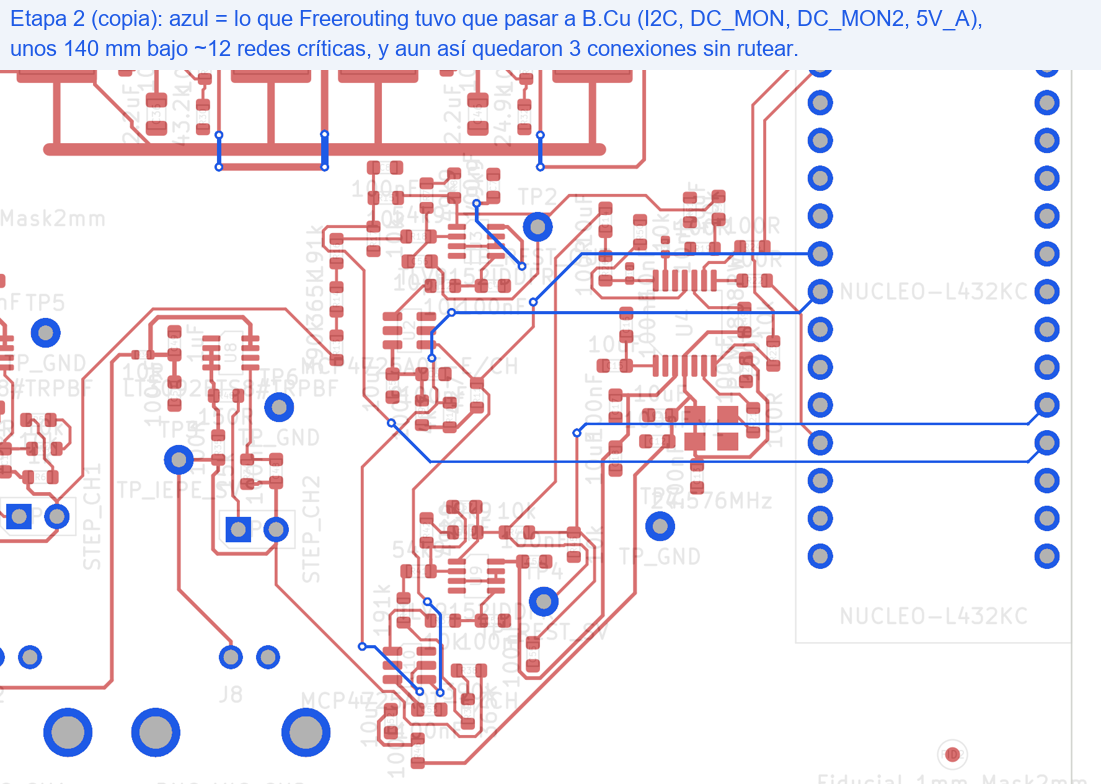
\includegraphics[width=0.92\linewidth]{figuras/oraculo_etapa2_bcu.png}
\caption{Oráculo, etapa 2 (copia de la placa): en azul lo que Freerouting tuvo que pasar a \capa{B.Cu} (I2C,
\net{DC_MON}, \net{DC_MON2}, \net{5V_A}). Son unos \SI{140}{\milli\meter} que cortan el plano debajo de unas 12 redes
críticas, y aun así quedaron 3 conexiones sin rutear.}
\label{fig:c08-oraculo}
\end{figure}

\subsection{La causa de fondo}

No era mala suerte con un par de pistas. Es la estructura del circuito sobre esta placa:
\begin{itemize}
  \item I2C, \net{DC_MON} y \net{DC_MON2} \textbf{nacen dentro de los dos AFE} (en el centro de la placa) y tienen que
  ir a la NUCLEO (a la derecha).
  \item Entre medio, las entradas del ADC y \net{REST_SV} bajan de arriba abajo: son una ``pared'' de señales críticas.
  \item \net{5V_A} y \net{3V3} salen de los buck (arriba) y tienen que entrar a grupos cerrados: \net{U3.8},
  \net{U9.8}, \net{U4.3}, el grupo de \net{3V3} del ADC y \net{C20}/\net{R49}.
\end{itemize}
Con la regla aprobada, cada una de esas redes lentas tendría que cruzar la pared por \capa{B.Cu}, debajo de señales
críticas y fuera de la zona digital, que es justo lo que la regla prohibía.

% =====================================================================================================
\section{Las opciones y la decisión}\label{sec:c08-opciones}

\begin{center}
\begin{tabularx}{\linewidth}{@{}L{0.17\linewidth}YY@{}}
\toprule
\textbf{Opción} & \textbf{Qué implica} & \textbf{Pros y contras} \\
\midrule
A: 2 capas con puentes cortos & Puentes de \SI{3}{\milli\meter} o menos, a \ang{90}, solo de rieles filtrados, I2C o redes
estáticas, y solo bajo señales de baja impedancia. & Más barata. Pero el ruteo es lento (cada puente se diseña y
justifica) y la etapa 2 mostró que no alcanzaba con puentes cortos. \\
A$'$: 2 capas con excepciones & Tramos largos de \capa{B.Cu} debajo de redes críticas (lo que hizo el oráculo). &
Rompe la regla justo en las señales que más la necesitan. \\
B: 4 capas & \capa{In1.Cu} plano GND entero; \capa{In2.Cu} alimentación y señales lentas; \capa{B.Cu} GND y señales
lentas. & Cumple la regla \textbf{sin excepciones de cruce}; no cambia placement ni esquemático; los bloques 1--3 ya
ruteados siguen valiendo. Cuesta más la placa desnuda. \\
C: recolocar la mitad derecha & Mover bloques enteros para que las redes no se crucen. & Cambio grande de placement
y sin garantía de solución. No se recomendó. \\
\bottomrule
\end{tabularx}
\end{center}

\begin{decision}[pasar a 4 capas (opción B)]
\textbf{Qué se decidió:} placa de 4 capas con el apilado estándar de JLCPCB (commit \texttt{3ccda8e}).

\textbf{Alternativas:} 2 capas con puentes (A), 2 capas con excepciones (A$'$) o recolocar bloques (C).

\textbf{Por qué:}
\begin{itemize}
  \item Con 2 capas la regla de cruces no tenía solución con el placement real (análisis a mano + oráculo).
  \item Con 4 capas, \capa{In1.Cu} es un plano GND \emph{entero} a \SI{0.21}{\milli\meter} debajo de todas las pistas
  de \capa{F.Cu}: cada señal crítica tiene su retorno justo debajo, y las redes lentas se cruzan por \capa{In2.Cu} y
  \capa{B.Cu} sin cortar ese plano.
  \item Es lo que hacen los diseños de referencia del fabricante: las placas de evaluación de TI del LMR36015 y del
  PCM1808 son de 4 capas \doc{REGLAS.md §6}, y el propio datasheet del LMR36015 une los dos pines \net{VIN} por una capa
  interna \doc{SNVSB49D fig.~12-2}.
  \item No obliga a tocar el placement ni el esquemático, y lo ruteado en los bloques 1--3 se conservó.
\end{itemize}

\textbf{Fuente:} \archivo{PLAN_RUTEO.md} §1, §2, §10 y §10.1.
\end{decision}

Lo que se ganó, en concreto: \textbf{cero excepciones a la regla de cruces}. Las únicas pistas que pasan por debajo
de otras son señales lentas en \capa{In2.Cu} y \capa{B.Cu}, y una herramienta comprueba que ninguna pase debajo de un
nodo protegido (sección~\ref{sec:c08-politica}).

% =====================================================================================================
\section{El apilado JLC04161H-7628}\label{sec:c08-apilado}

``Apilado'' (\emph{stackup}) es cómo están ordenadas y separadas las capas de cobre dentro de la placa. JLCPCB tiene
apilados estándar; para 4 capas y \SI{1.6}{\milli\meter} el que se usó es el JLC04161H-7628. El ensamblaje económico
de JLCPCB solo acepta apilados estándar \doc{página de capacidades PCBA}.

\begin{figure}[htbp]
\centering
\begin{tikzpicture}[yscale=6,xscale=1]
  % de abajo hacia arriba, en mm
  \def\cu{0.035}\def\pp{0.2104}\def\inn{0.0152}\def\core{1.065}
  \pgfmathsetmacro{\yA}{0}
  \pgfmathsetmacro{\yB}{\cu}
  \pgfmathsetmacro{\yC}{\cu+\pp}
  \pgfmathsetmacro{\yD}{\cu+\pp+\inn}
  \pgfmathsetmacro{\yE}{\cu+\pp+\inn+\core}
  \pgfmathsetmacro{\yF}{\cu+\pp+2*\inn+\core}
  \pgfmathsetmacro{\yG}{\cu+2*\pp+2*\inn+\core}
  \pgfmathsetmacro{\yH}{2*\cu+2*\pp+2*\inn+\core}
  \fill[cobre] (0,\yA) rectangle (4.5,\yB);
  \fill[green!25!black!12] (0,\yB) rectangle (4.5,\yC);
  \fill[orange!80!black] (0,\yC) rectangle (4.5,\yD);
  \fill[green!25!black!20] (0,\yD) rectangle (4.5,\yE);
  \fill[verdeplaca!80] (0,\yE) rectangle (4.5,\yF);
  \fill[green!25!black!12] (0,\yF) rectangle (4.5,\yG);
  \fill[cobre] (0,\yG) rectangle (4.5,\yH);
  \node[anchor=west,font=\footnotesize] at (4.7,\yH-0.0175) {\capa{F.Cu} \SI{0.035}{\milli\meter} (1 oz): piezas y señales críticas};
  \node[anchor=west,font=\footnotesize] at (4.7,\yF/2+\yG/2) {prepreg 7628 \SI{0.2104}{\milli\meter}, $\varepsilon_r \approx \num{4.4}$};
  \node[anchor=west,font=\footnotesize] at (4.7,\yF+0.02) {\capa{In1.Cu} \SI{0.0152}{\milli\meter}: GND entero};
  \node[anchor=west,font=\footnotesize] at (4.7,\yD/2+\yE/2) {núcleo \SI{1.065}{\milli\meter}, $\varepsilon_r \approx \num{4.6}$};
  \node[anchor=west,font=\footnotesize] at (4.7,\yD-0.02) {\capa{In2.Cu} \SI{0.0152}{\milli\meter}: alimentación y lentas};
  \node[anchor=west,font=\footnotesize] at (4.7,\yB/2+\yC/2) {prepreg 7628 \SI{0.2104}{\milli\meter}};
  \node[anchor=west,font=\footnotesize] at (4.7,\yA+0.0175) {\capa{B.Cu} \SI{0.035}{\milli\meter} (1 oz): GND y lentas};
  \draw[|-|] (-0.3,\yA) -- node[left,font=\small]{$\approx$\SI{1.6}{\milli\meter}} (-0.3,\yH);
\end{tikzpicture}
\caption{Apilado JLC04161H-7628 dibujado a escala vertical (los cobres internos son tan finos que casi no se ven).
Espesores y permitividades de la página de impedancia de JLCPCB \doc{REGLAS.md §9}. Fíjate que \capa{In1.Cu} está muy
cerca de \capa{F.Cu} (un prepreg) y lejos de \capa{In2.Cu} (el núcleo).}
\label{fig:c08-apilado}
\end{figure}

Lo más importante del dibujo es la distancia de \capa{F.Cu} a \capa{In1.Cu}: \SI{0.2104}{\milli\meter}. Cuanto más
cerca está el plano, más pegado va el retorno debajo de la pista y más chico es el lazo (figura~\ref{fig:c08-corte}).
En 2 capas, el plano (\capa{B.Cu}) habría quedado al otro lado de toda la placa, a casi \SI{1.5}{\milli\meter}
\estimado{}. Por eso las señales críticas van en
\capa{F.Cu}, la capa que tiene el plano más cerca.

\subsection{Para qué se usa cada capa}

\begin{center}
\begin{tabularx}{\linewidth}{@{}L{0.14\linewidth}YL{0.2\linewidth}@{}}
\toprule
\textbf{Capa} & \textbf{Uso} & \textbf{Pistas \medido} \\
\midrule
\capa{F.Cu} & Piezas y todas las redes críticas; relleno GND cosido en lo que queda libre; zonas de
\SI{24}{\volt}, \net{SW} y salidas de los buck. & \SI{925}{\milli\meter} \\
\capa{In1.Cu} & GND entero, \textbf{sin ninguna pista}. Es la referencia de todo \capa{F.Cu}. & \SI{0}{\milli\meter} \\
\capa{In2.Cu} & Distribución de \net{3V3} y \net{5V_A} (pistas de \SI{0.4}{\milli\meter}), I2C del canal 2, un tramo de
\net{DC_MON2} y los straps \net{MD1}/\net{FMT} del ADC. & \SI{302}{\milli\meter} \\
\capa{B.Cu} & Zona GND más señales lentas: I2C del canal 1, \net{DC_MON}, \net{DC_MON2} y los tres puentes cortos bajo
el bus de \SI{24}{\volt}. & \SI{253}{\milli\meter} \\
\bottomrule
\end{tabularx}
\end{center}

\begin{figure}[htbp]
\centering
\begin{tabular}{@{}c@{\hspace{4mm}}c@{}}
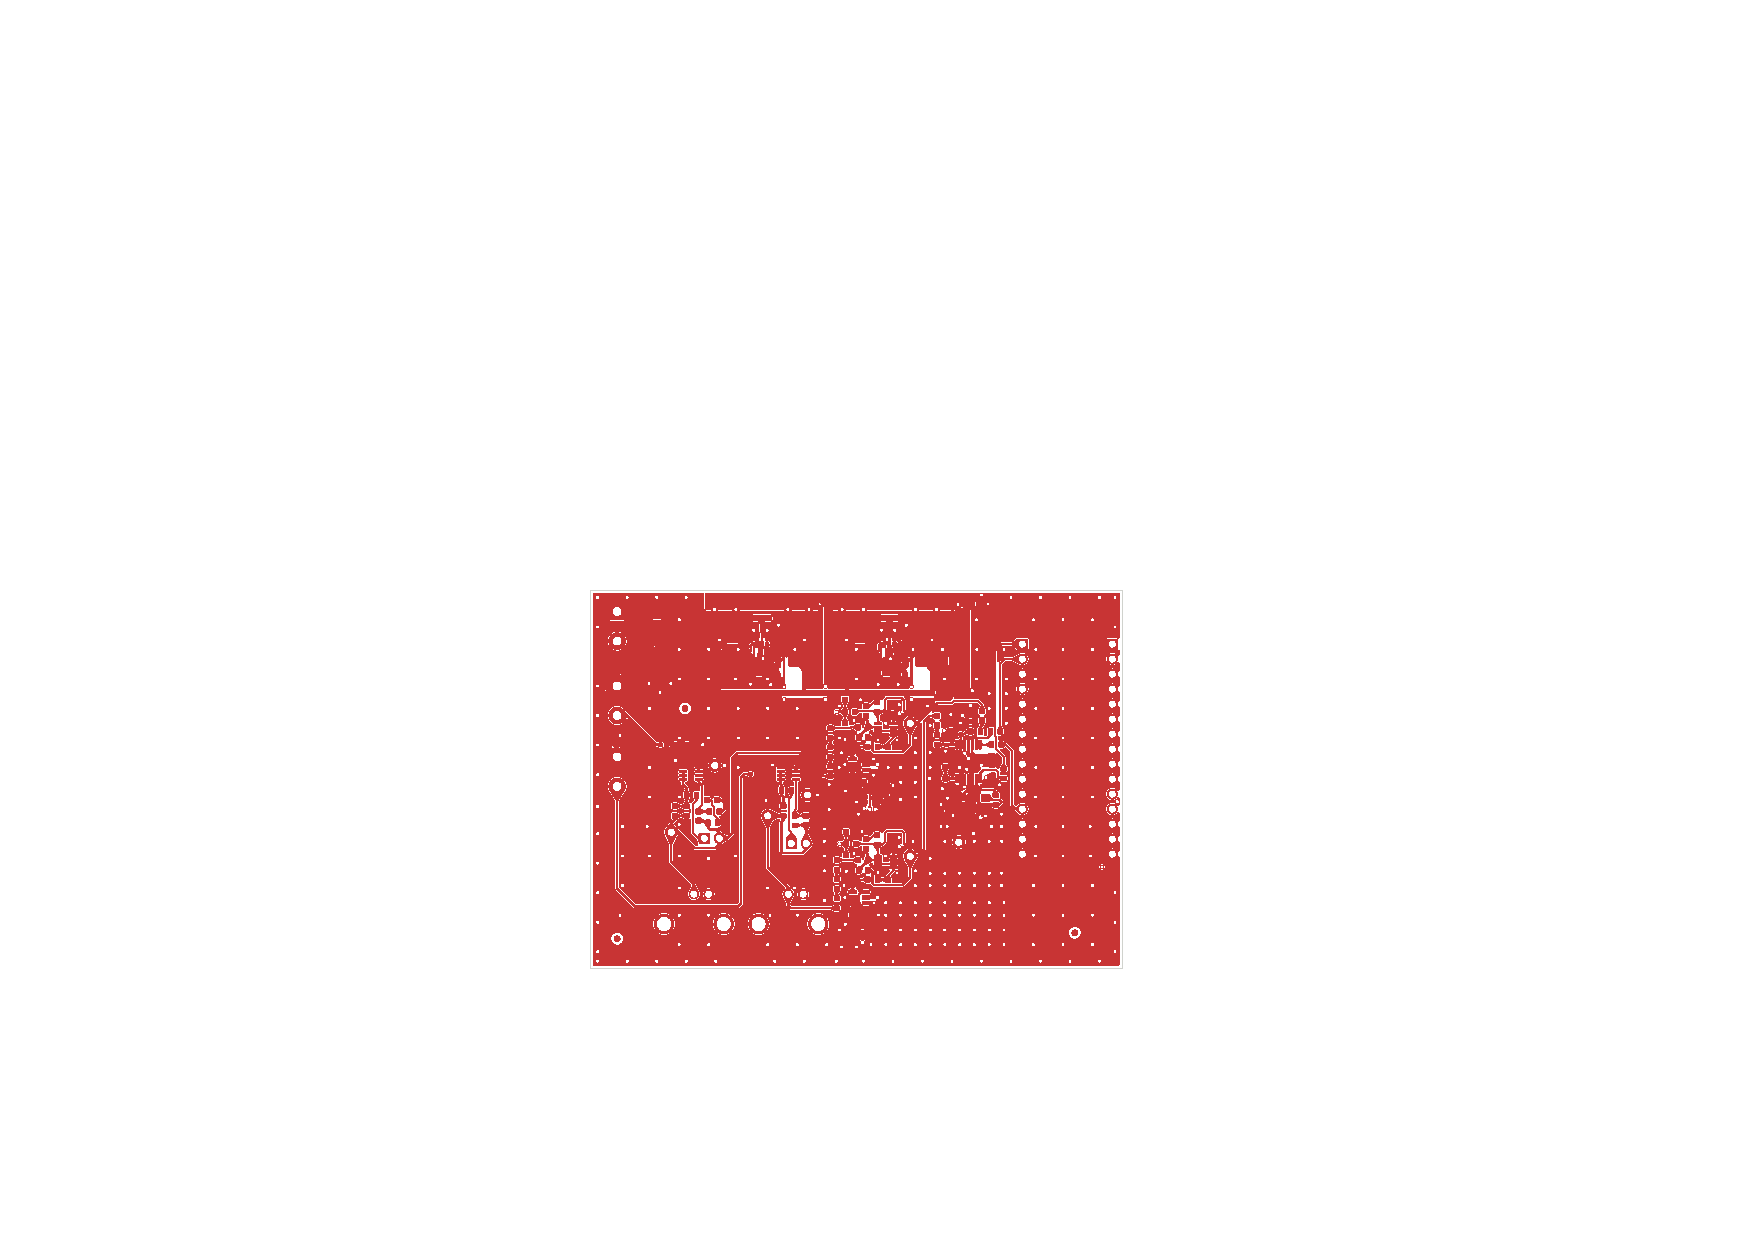
\includegraphics[width=0.47\linewidth]{figuras/capa_F_Cu.pdf} &
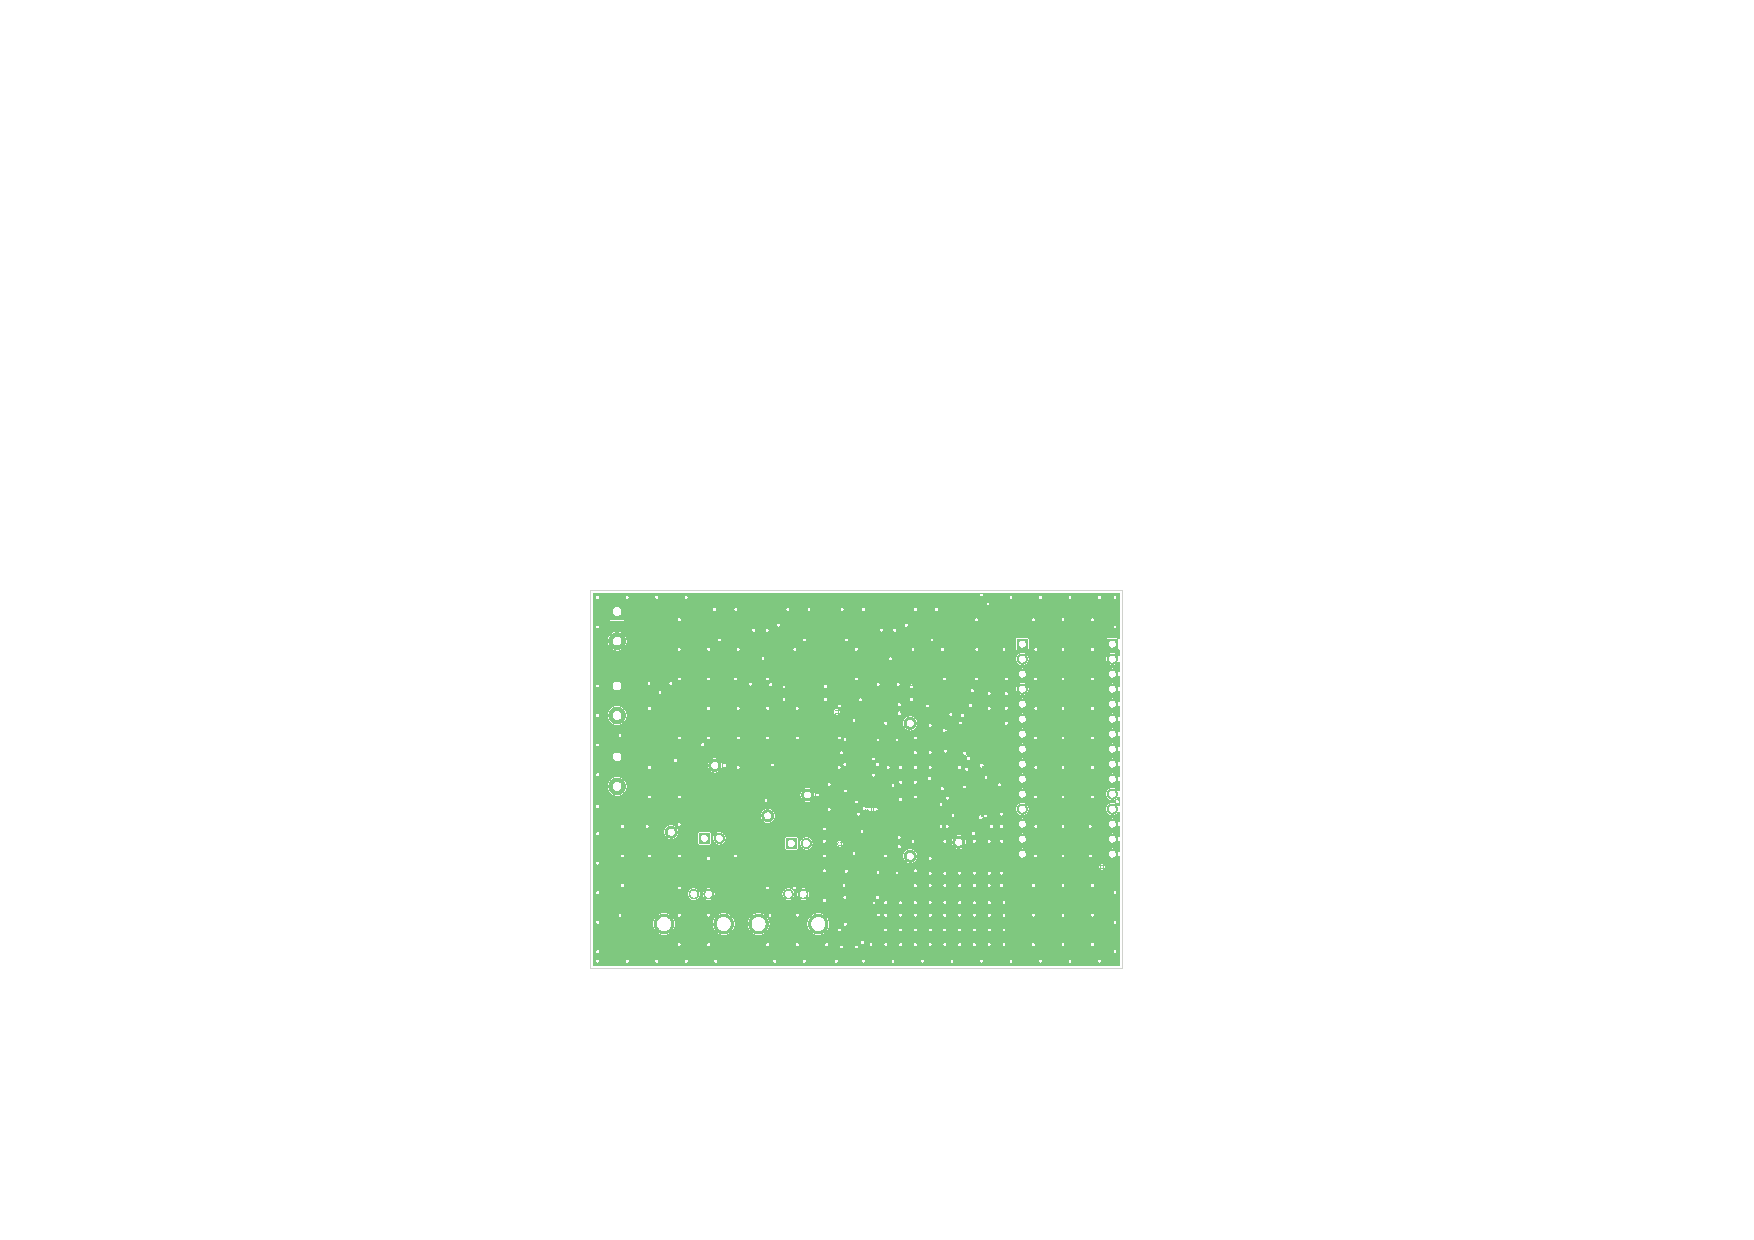
\includegraphics[width=0.47\linewidth]{figuras/capa_In1_Cu.pdf} \\
\small (a) \capa{F.Cu} & \small (b) \capa{In1.Cu} \\[3mm]
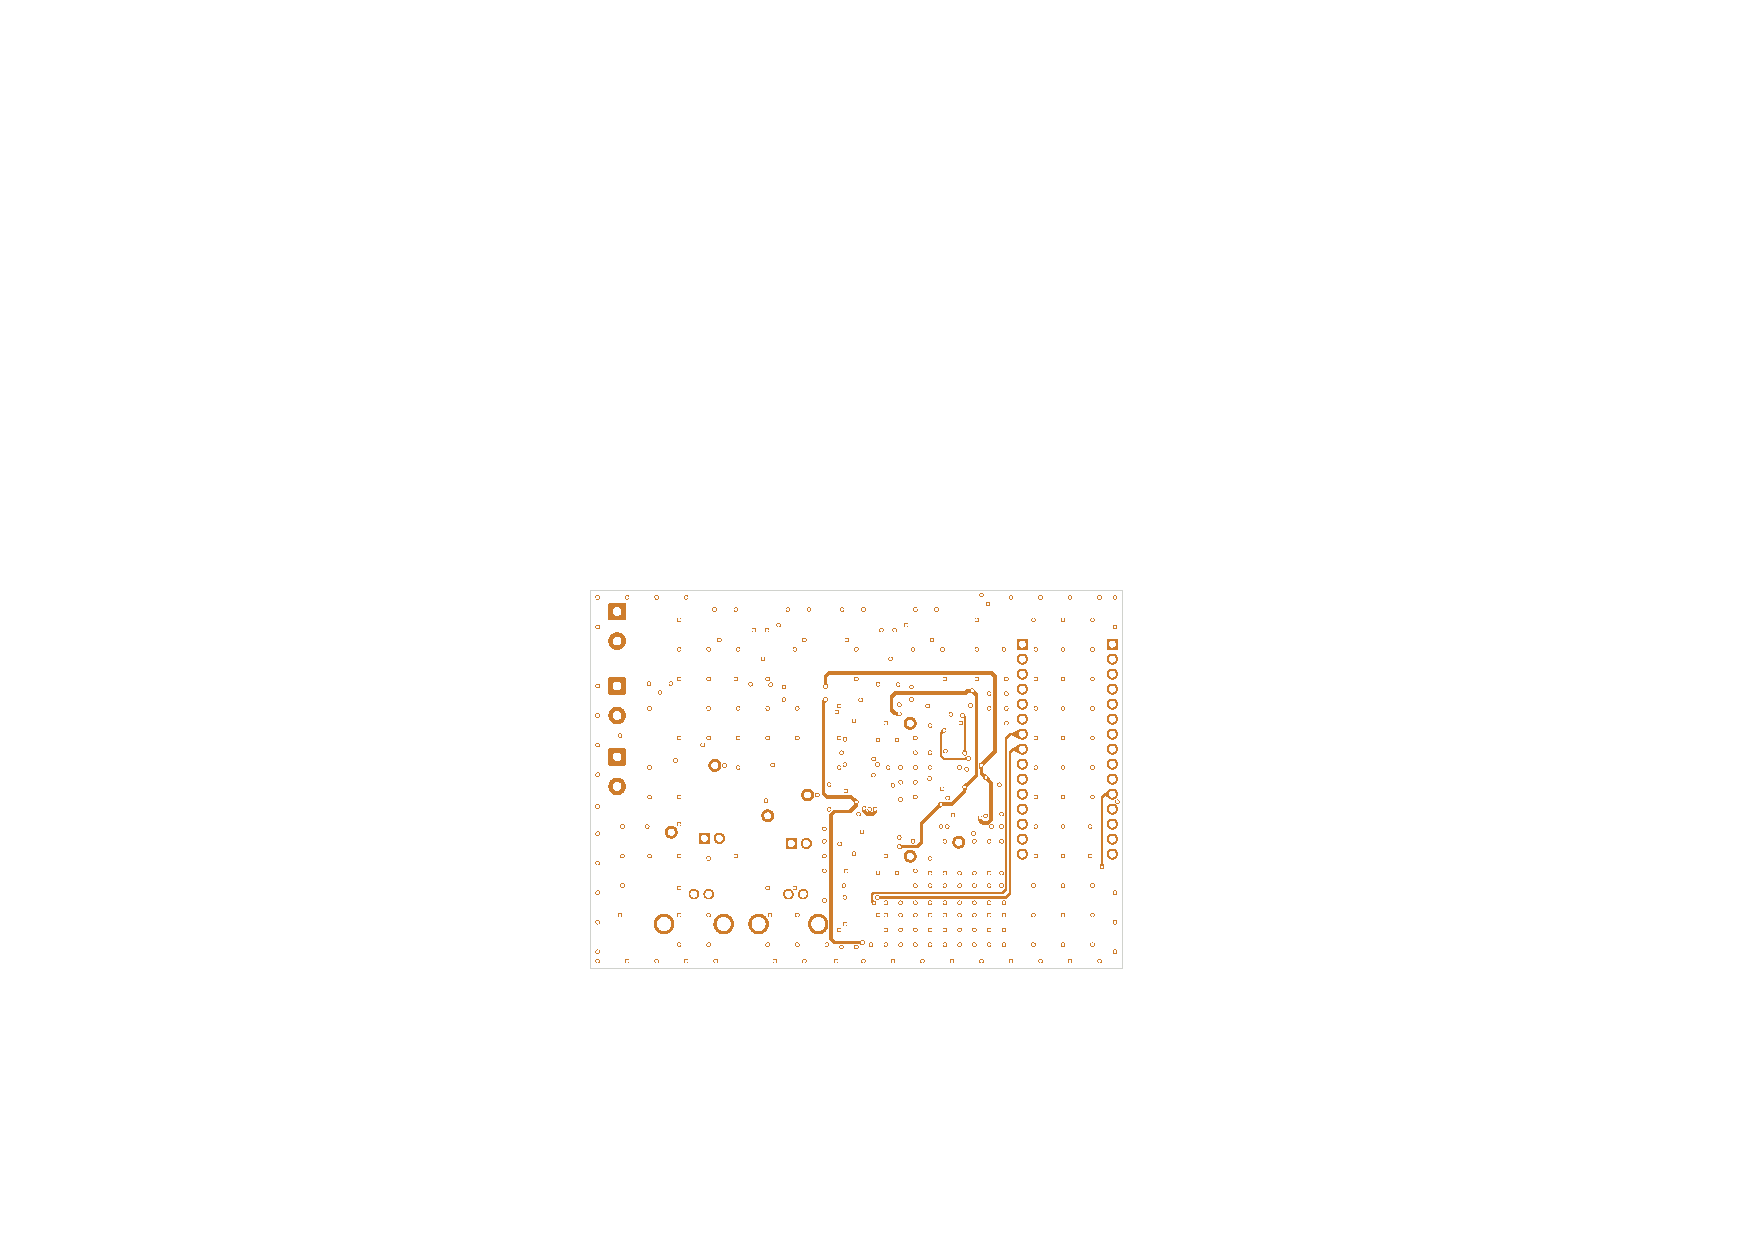
\includegraphics[width=0.47\linewidth]{figuras/capa_In2_Cu.pdf} &
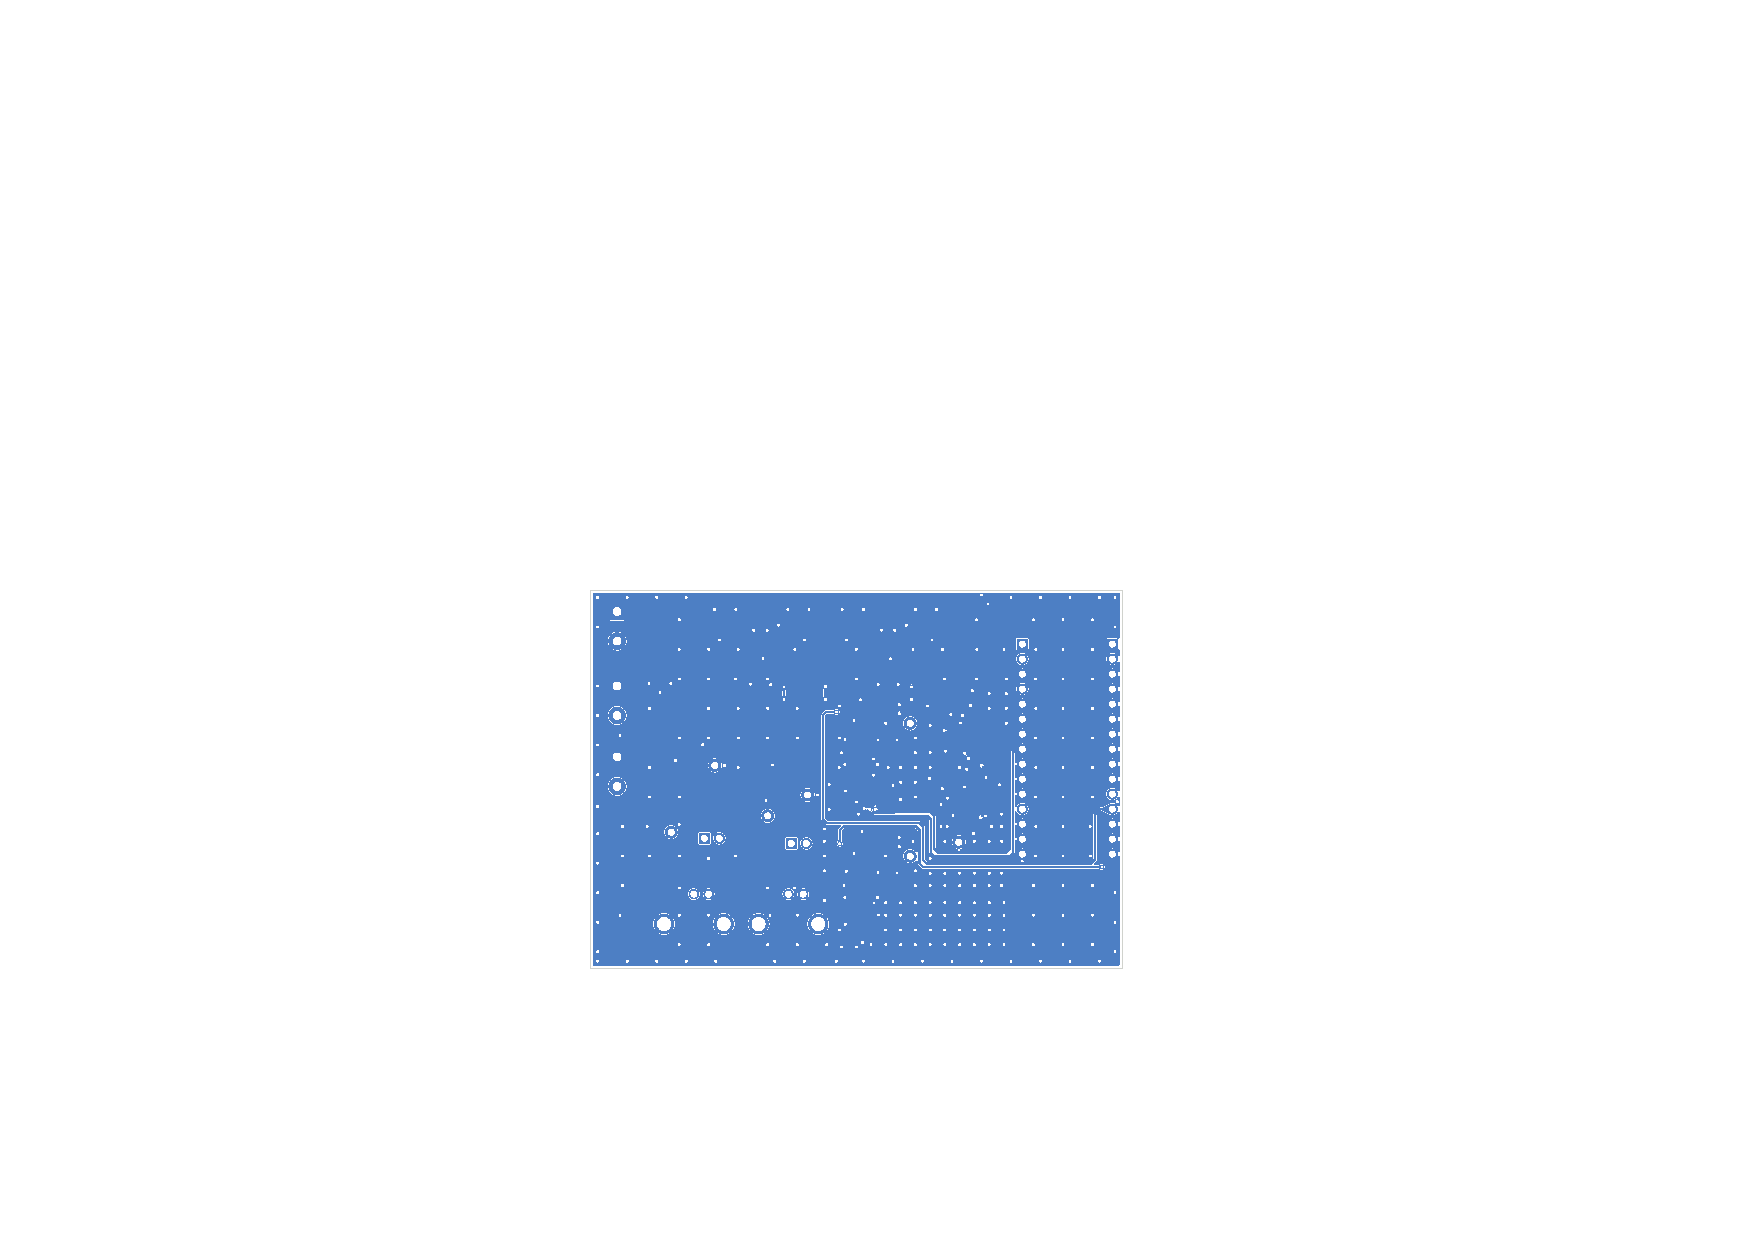
\includegraphics[width=0.47\linewidth]{figuras/capa_B_Cu.pdf} \\
\small (c) \capa{In2.Cu} & \small (d) \capa{B.Cu}
\end{tabular}
\caption{Las cuatro capas de cobre de la placa terminada (vista desde arriba, exportadas con \texttt{kicad-cli}).
(a) \capa{F.Cu}: casi todo es relleno GND; las pistas se ven como líneas blancas (las separaciones) y arriba están las
zonas de los dos buck. (b) \capa{In1.Cu}: plano GND entero; los puntos son las holguras de las vías y de los pines con
agujero. (c) \capa{In2.Cu}: solo pistas, sin plano: \net{3V3} y \net{5V_A} bajando desde los buck, y el I2C del canal 2
y \net{DC_MON2} llegando a la NUCLEO (columnas de pines a la derecha). (d) \capa{B.Cu}: zona GND con las pistas lentas
(I2C del canal 1, \net{DC_MON}, \net{DC_MON2}) recortadas en ella.}
\label{fig:c08-capas}
\end{figure}

% =====================================================================================================
\section{Cómo se verifica que se respete el uso de las capas}\label{sec:c08-politica}

Decidir el uso de cada capa no sirve de nada si no se comprueba. Se hizo con dos herramientas propias que leen la
placa con la API de KiCad (detalles en el capítulo~\ref{cap:verif}):

\begin{itemize}
  \item \textbf{Chequeo G de \archivo{revisar_pistas.py}:} \capa{In1.Cu} sin pistas (plano entero); las redes de clase
  Analógica, Reloj y Conmutado solo en \capa{F.Cu}, con dos excepciones: \net{DC_MON}/\net{DC_MON2} (son un nivel de
  DC filtrado) e \net{IEPE_FEED*} (el riel de \SI{24}{\volt} de cada fuente IEPE, que es DC). \capa{In2.Cu} y
  \capa{B.Cu} quedan para alimentación y señales lentas.
  \item \textbf{Chequeo I:} recorre cada pista crítica de \capa{F.Cu} y comprueba que debajo, en \capa{In1.Cu}, haya
  cobre GND continuo (contra el relleno real de la zona). Los únicos huecos permitidos son el anillo libre alrededor de
  un pad con agujero o de una vía de la misma red, justo donde la pista termina.
  \item \textbf{\archivo{cruces_capas.py}:} para cada pista de \capa{In2.Cu} y \capa{B.Cu} lista qué cobre de
  \capa{F.Cu} tiene encima. Marca como error si pasa debajo de un nodo protegido: los nodos \net{SUM}, el nodo filtrado
  del DAC, la cadena de \SI{1}{\mega\ohm} y el nodo medio de la realimentación. Resultado final: \textbf{0 cruces bajo
  nodos protegidos}; lo que queda encima de pistas de otras capas son \net{IEPE}, \net{REST_SV}, las líneas SAI y el
  I2C, todas de baja impedancia.
\end{itemize}

\begin{ojo}[por qué esta regla sigue valiendo con 4 capas]
Con \capa{In1.Cu} entero podrías pensar que ya da igual qué pase por \capa{In2.Cu} o \capa{B.Cu}. Para el retorno sí da
igual, porque el retorno de \capa{F.Cu} va por \capa{In1.Cu}, y el plano además hace de pantalla entre las capas. Pero
el plano no es perfecto: tiene holguras alrededor de cada vía y de cada pin con agujero. Con nodos de cientos de
k$\Omega$ (sección~\ref{sec:c08-altaz}) se prefirió no depender de eso, y la regla del dueño de los bloques 3 y 4 se
mantuvo. Respetarla no costó nada: el ruteo encontró camino para todas las redes lentas sin pasar bajo esos nodos.
\end{ojo}

% =====================================================================================================
\section{Cuánto cuesta y si sirve para el ensamblaje económico}\label{sec:c08-costo}

Cotización de JLCPCB sin sesión iniciada, sin envío ni ensamblaje, para 5 placas de \qtyproduct{90 x 64}{\milli\meter},
4 capas, \SI{1.6}{\milli\meter} y máscara verde \doc{REGLAS.md §9, cotizador JLCPCB, 2026-11-16}:

\begin{center}
\begin{tabular}{@{}lr@{}}
\toprule
\textbf{Acabado} & \textbf{Precio (5 placas)} \\
\midrule
HASL con plomo (oferta) & USD \num{8.00} \\
\textbf{HASL sin plomo (elegido)} & \textbf{USD \num{13.20}} \\
ENIG & USD \num{25.30} \\
\bottomrule
\end{tabular}
\end{center}

La versión de 2 capas de esta misma placa no se cotizó, así que no hay una diferencia de precio medida; las cifras de
blogs que se vieron al principio son de terceros y no se verificaron \copia. Lo que sí se comprobó es que el cambio no
saca a la placa del ensamblaje económico (\emph{Economic PCBA}): en la tabla de capacidades de JLCPCB, la fila de
Economic dice ``4L · 1.6 · Green · Lead-Free:HASL / ENIG · 2--50'' \doc{página de capacidades PCBA, 2026-11-16}, y la
misma página acepta 2, 4 y 6 capas, espesores de \SIrange{0.8}{1.6}{\milli\meter} y ``solo apilado estándar''.

\begin{ojo}[vías taponadas: una consecuencia directa de las 4 capas]
En placas de 4 capas JLCPCB tapona las vías por defecto (\emph{plugged}), y una vía a menos de \SI{0.35}{\milli\meter}
de un pad no se puede taponar con tinta \doc{JLCPCB, artículo de recubrimiento de vías}. Por eso, al pasar a 4 capas,
apareció una regla nueva (\texttt{via\_tapada\_lejos\_de\_pad}) y hubo que mover 43 vías ya puestas. Lo ves en el
capítulo~\ref{cap:ruteo}.
\end{ojo}

\section*{Resumen}
\begin{itemize}
  \item Toda señal forma un lazo con su retorno por tierra; a alta frecuencia el retorno va justo debajo de la pista, y
  el área del lazo decide cuánto ruido capta, emite y acopla.
  \item Un corte en el plano obliga al retorno a rodear y agranda el lazo. En 2 capas, cada pista en \capa{B.Cu} es un
  corte en el plano.
  \item Los nodos de la cadena de \SI{1}{\mega\ohm} tienen cientos de k$\Omega$: una capacidad parásita de
  \SI{0.1}{\pico\farad} ya deja pasar un 15\,\% de un ruido de \SI{1}{\mega\hertz}.
  \item La regla de 2 capas (plano en \capa{B.Cu}, críticas solo en \capa{F.Cu}) no tenía solución con el placement
  real: I2C y \net{DC_MON} nacen en los AFE y van a la NUCLEO cruzando una pared de señales críticas. El oráculo
  (Freerouting en copias) lo confirmó: 3 conexiones sin rutear aun usando \SI{140}{\milli\meter} de \capa{B.Cu} bajo
  12 redes críticas.
  \item Se eligió 4 capas: \capa{In1.Cu} es un plano GND entero a \SI{0.21}{\milli\meter} de \capa{F.Cu}, y las
  redes lentas se cruzan por \capa{In2.Cu} y \capa{B.Cu}. Resultado: cero excepciones de cruce y cero pistas bajo
  nodos protegidos.
  \item Cuesta USD \num{13.20} por 5 placas con HASL sin plomo y sigue siendo compatible con el ensamblaje económico de
  JLCPCB.
\end{itemize}

\chapter{Cómo se ruteó la placa}\label{cap:ruteo}

% colores y estilos de las figuras generadas desde la placa (figuras/c09_*.tex)
\colorlet{fondo}{verdeplaca!6}\colorlet{padfill}{black!18}\colorlet{paddraw}{black!55}
\colorlet{cSW}{red!80!black}\colorlet{c24}{orange!90!black}\colorlet{cOut}{green!50!black}
\colorlet{cGND}{black!70}\colorlet{cSig}{blue!70!black}\colorlet{cIn}{violet}\colorlet{cB}{cyan!60!black}
\tikzset{etiq/.style={font=\sffamily\tiny\bfseries,text=black,fill=white,fill opacity=0.7,text opacity=1,inner sep=0.6pt}}

Con el placement fijo (capítulo~\ref{cap:placement}) y la placa ya en 4 capas (capítulo~\ref{cap:capas}), faltaba
lo más largo: dibujar las pistas. Aquí vas a ver las reglas que siguió cada pista, por qué existe cada regla, cómo se
dibujó la placa (no con un autorouter) y qué se decidió en cada uno de los diez bloques del ruteo.

\textbf{En este capítulo vas a ver:}
\begin{itemize}
  \item el método: pistas escritas como listas de puntos, por bloques, con verificación después de cada bloque;
  \item las reglas de trazado, una por una, con su porqué y cómo se comprueba;
  \item anchos de pista, separaciones, zonas de cobre y vías de cosido;
  \item el recorrido bloque por bloque, desde los buck hasta los teardrops y la serigrafía;
  \item en qué orden hay que correr los pasos finales y por qué ese orden importa.
\end{itemize}

% =====================================================================================================
\section{El método: polilíneas por bloques}\label{sec:c09-metodo}

\subsection{Por qué no un autorouter}

Un autorouter (como Freerouting) encuentra caminos, pero no entiende el circuito: no sabe que el lazo de entrada de un
buck tiene que ser diminuto, que un condensador de desacoplo tiene que ir pegado al pin, que el nodo \net{SUM} no
puede tener nada debajo, ni que una pista debe entrar al pad por el centro. Además deja quiebres, vías y desvíos que
luego hay que limpiar a mano. Por eso Freerouting solo se usó como \emph{oráculo} en copias de la placa, para
preguntar si existía solución con una regla (capítulo~\ref{cap:capas}). El ruteo real se hizo a mano.

\subsection{``A mano'', pero escrito como datos}

``A mano'' no quiere decir con el mouse en KiCad. Cada pista se escribió como una lista de puntos de paso (coordenadas
de KiCad en mm) en un archivo de Python por bloque. Los archivos están en la carpeta
\archivo{tools/ruteo/bloques/}. Por ejemplo, el comienzo del bloque 2 (entrada de \SI{24}{\volt}) se ve así:

\begin{small}
\begin{verbatim}
PISTAS = [
    # 24V_IN: J5.1 -> D1.2 (ánodo), recto
    ('Net-(D1-A)', 1.0, 'F.Cu', [(104.5, 103.6), (111.25, 103.6)]),
    # 24V_PROT: D1.1 (cátodo) -> D2.1
    ('24V_PROT', 1.0, 'F.Cu', [(111.25, 107.6), (111.25, 108.95),
                              (111.75, 109.45), (111.75, 110.95)]),
    ...
\end{verbatim}
\end{small}

Cada entrada es (red, ancho en mm, capa, puntos). Hay listas iguales para las vías (\texttt{VIAS}) y las zonas
(\texttt{ZONAS}). El script \archivo{tools/ruteo/polilineas.py} lee el bloque y lo escribe en la placa con la API de
KiCad (\texttt{pcbnew}). Antes de escribir nada \textbf{valida el bloque}: cada segmento tiene que ser múltiplo de
\ang{45}, medir al menos \SI{0.1}{\milli\meter} y girar \ang{0} o \ang{45} respecto del anterior. Si el bloque no es
válido, no toca la placa.

\begin{idea}[por qué escribir las pistas como datos]
\begin{itemize}
  \item \textbf{Se puede rehacer un bloque sin tocar el resto.} Cada bloque se guarda en un grupo de KiCad
  (\texttt{ruteo:<bloque>}). Al volver a aplicarlo, el script borra lo que tenía ese grupo y lo vuelve a escribir.
  \item \textbf{Cada coordenada tiene un comentario} que dice por qué la pista pasa por ahí (``entre los pads de
  \net{R22} y \net{R24}, \SI{0.325}{\milli\meter} a cada lado'').
  \item \textbf{Es revisable y repetible}: el ruteo queda en git como texto, y cualquier cambio se ve en un diff.
\end{itemize}
\end{idea}

\subsection{Verificar después de cada bloque}

Después de cada bloque se corrió \archivo{tools/ruteo/verificar_bloque.py}, que hace siempre lo mismo:
\begin{enumerate}
  \item DRC de KiCad con paridad esquemático--placa, todas las severidades, rellenando las zonas y guardando el relleno;
  \item ERC del esquemático;
  \item \archivo{revisar_pistas.py}, el revisor propio con los chequeos A--M (lo que el DRC no ve);
  \item imágenes de cada capa para mirar a ojo.
\end{enumerate}
Solo con todo en cero se hacía commit y se pasaba al bloque siguiente. Después del bloque 1 hubo una parada
obligatoria para que el dueño revisara en KiCad. El detalle de estas herramientas está en el capítulo~\ref{cap:verif}.

% =====================================================================================================
\section{Las reglas de trazado, una por una}\label{sec:c09-reglas}

\subsection{Solo ángulos de 45°}

\textbf{Qué:} cada segmento de pista es horizontal, vertical o diagonal a \ang{45}, y dos segmentos seguidos forman un
ángulo interior de \ang{135} o más. Nada de esquinas de \ang{90} ni agudas.

\textbf{Por qué:} a las frecuencias de esta placa una esquina de \ang{90} no cambia el comportamiento eléctrico de forma
apreciable, así que el motivo no es ``la esquina radia''. Los motivos reales son de fabricación y de orden: un ángulo
agudo deja una cuña estrecha de cobre o de separación que es difícil de grabar bien; las diagonales acortan los
recorridos frente a dos tramos a \ang{90}; y una regla uniforme hace la placa fácil de revisar. Además era una regla
pedida por el dueño.

\textbf{Cómo se comprueba:} con la regla propia \texttt{solo\_45} del archivo \archivo{pcb.kicad_dru}
(\texttt{track\_angle} mínimo de \ang{135}, error en el DRC), con la validación de \archivo{polilineas.py} y con los
chequeos A y B de \archivo{revisar_pistas.py}.

\begin{figure}[htbp]
\centering
\begin{tikzpicture}[scale=0.9]
  \begin{scope}
    \draw[line width=3pt,cobre] (0,0) -- (1.5,0) -- (2.5,1) -- (2.5,2);
    \node[font=\small,green!40!black] at (1.3,-0.5) {bien: \ang{135}};
  \end{scope}
  \begin{scope}[xshift=4cm]
    \draw[line width=3pt,cobre] (0,0) -- (2,0) -- (2,2);
    \node[font=\small,rojoojo] at (1.2,-0.5) {mal: \ang{90}};
  \end{scope}
  \begin{scope}[xshift=8cm]
    \draw[line width=3pt,cobre] (0,0) -- (2,0) -- (0.8,1.2);
    \node[font=\small,rojoojo] at (1.1,-0.5) {mal: \ang{45} (agudo)};
  \end{scope}
\end{tikzpicture}
\caption{Esquinas permitidas y prohibidas. La regla mide el ángulo \emph{interior} entre los dos segmentos.}
\label{fig:c09-angulos}
\end{figure}

\subsection{Entrar al pad por el centro y por su eje}

\textbf{Qué:} la pista termina en el centro del pad y llega paralela a uno de sus ejes. Si tiene que girar, el quiebre
queda \emph{fuera} del pad.

\textbf{Por qué:} el pad de un componente pequeño (un 0402 o un 0603) es casi del tamaño de la pista. Si la pista
entra en diagonal o por una esquina, el cobre ``visible'' del pad cambia de forma: la soldadura moja distinto a cada
lado y en las piezas chicas eso favorece que el componente se levante de un lado (efecto lápida o
\emph{tombstoning}). Entrar por el eje y por el centro hace que los dos pads de una pieza se vean iguales para la
soldadura. Además, una pista que sale de un pin fino con el ancho del pad no deja esquinas de cobre fuera del pad.

\textbf{Cómo se comprueba:} chequeo C de \archivo{revisar_pistas.py}. Hubo una sola excepción aceptada, el enlace del
nodo \net{SUM} entre el condensador de realimentación y la resistencia de entrada (bloque 5).

\begin{figure}[htbp]
\centering
\begin{tikzpicture}[scale=0.9]
  \tikzset{pad/.style={fill=black!18,draw=black!55,rounded corners=1pt}}
  \begin{scope}
    \draw[pad] (0,0) rectangle (1,1.2);
    \draw[line width=4pt,cobre] (0.5,0.6) -- (2.5,0.6) -- (3.3,1.4);
    \fill (0.5,0.6) circle (0.05);
    \node[font=\small,green!40!black,align=center] at (1.6,-0.5) {bien: llega por el eje,\\quiebre fuera del pad};
  \end{scope}
  \begin{scope}[xshift=5cm]
    \draw[pad] (0,0) rectangle (1,1.2);
    \draw[line width=4pt,cobre] (0.5,0.6) -- (1.8,1.9);
    \node[font=\small,rojoojo,align=center] at (1.1,-0.5) {mal: entra\\en diagonal};
  \end{scope}
  \begin{scope}[xshift=9cm]
    \draw[pad] (0,0) rectangle (1,1.2);
    \draw[line width=4pt,cobre] (0.9,0.2) -- (2.5,0.2);
    \node[font=\small,rojoojo,align=center] at (1.3,-0.5) {mal: termina\\fuera del centro};
  \end{scope}
\end{tikzpicture}
\caption{Entrada de una pista a un pad. Solo la primera cumple el chequeo C.}
\label{fig:c09-entrada}
\end{figure}

\subsection{Sin \emph{stubs}}

\textbf{Qué:} ninguna pista termina en el aire ni sigue de largo después de su último punto de conexión. Tampoco hay
segmentos duplicados o superpuestos, ni vías que no conecten al menos dos capas.

\textbf{Por qué:} un tramo que no lleva a ningún lado (\emph{stub}) no conduce corriente útil, pero sí tiene capacidad y
se comporta como una pequeña antena que capta ruido. En señales rápidas, un stub refleja la señal. Y casi siempre es
un error: un pedazo de pista que quedó de una edición anterior.

\textbf{Cómo se comprueba:} chequeos E y F de \archivo{revisar_pistas.py} y las reglas \texttt{track\_dangling} y
\texttt{via\_dangling} del DRC, configuradas como error.

\subsection{Ramificar solo en pads o en zonas}

\textbf{Qué:} si una red tiene que repartirse a varias piezas, la división se hace en el pad de una pieza (o en una
zona de cobre), nunca en medio de una pista.

\textbf{Por qué:} una ``T'' en medio de una pista crea un ángulo de \ang{90} entre ramas, y con tres ramas en un punto
no pueden quedar todas a \ang{135} o más entre sí. El DRC de KiCad mide eso con \texttt{track\_angle} y lo marca. Se
descubrió al probar el bus de \SI{24}{\volt} en una copia de la placa: una unión en T sobre pista desnuda la marcó el DRC.

Hubo un caso más sutil en el bloque 8: la regla \texttt{track\_angle} también mira las uniones \emph{en vías}. Una vía
con tres pistas en la misma capa tiene el mismo problema que la T. Por eso el pad \net{R9.2} tiene \textbf{dos vías}
unidas por \capa{F.Cu}, y de cada una sale una sola rama.

\begin{figure}[htbp]
\centering
\begin{tikzpicture}[scale=0.9]
  \tikzset{pad/.style={fill=black!18,draw=black!55,rounded corners=1pt}}
  \begin{scope}
    \draw[line width=3pt,cobre] (0,0) -- (3,0);
    \draw[line width=3pt,cobre] (1.5,0) -- (1.5,1.4);
    \node[font=\small,rojoojo] at (1.5,-0.5) {mal: T en pista};
  \end{scope}
  \begin{scope}[xshift=5cm]
    \draw[pad] (1.1,-0.4) rectangle (1.9,0.4);
    \draw[line width=3pt,cobre] (0,0) -- (1.5,0) -- (3,0);
    \draw[line width=3pt,cobre] (1.5,0) -- (1.5,1.4);
    \node[font=\small,green!40!black] at (1.5,-0.8) {bien: la unión es el pad};
  \end{scope}
\end{tikzpicture}
\caption{Una ramificación en pista libre deja un ángulo de \ang{90}. Si la unión cae en el centro de un pad, la
``esquina'' queda dentro del cobre del pad y no hay ángulo de pista.}
\label{fig:c09-t}
\end{figure}

\subsection{Teardrops}

\textbf{Qué:} un \emph{teardrop} (lágrima) es un relleno triangular de cobre en la unión entre una pista y un pad o una
vía, que ensancha la pista justo antes de llegar.

\textbf{Por qué:} la unión pista--pad es el punto mecánicamente más débil. Si el taladro sale un poco corrido (todos los
fabricantes tienen tolerancia de registro), el anillo de cobre alrededor del agujero puede quedar muy angosto justo
donde llega la pista, y la pista se puede cortar. El teardrop agrega cobre ahí y también reparte el esfuerzo térmico y
mecánico.

\textbf{Cómo se hizo:} \archivo{tools/ruteo/teardrops.py} activa los teardrops en todos los pads con red y en todas las
vías, con los parámetros por defecto de KiCad 10. No hace falta abrir KiCad: el DRC por línea de comandos con
\texttt{-{}-refill-zones -{}-save-board} genera las zonas de teardrop. Resultado: \textbf{440 teardrops} \medido.

\begin{figure}[htbp]
\centering
\begin{tikzpicture}[scale=1]
  \begin{scope}
    \fill[black!18] (0,0) circle (0.6); \fill[white] (0,0) circle (0.25);
    \draw[line width=4pt,cobre] (0.5,0) -- (2.6,0);
    \node[font=\small] at (1.2,-0.9) {sin teardrop};
  \end{scope}
  \begin{scope}[xshift=4.5cm]
    \fill[cobre!70] (0.35,0.45) .. controls (0.9,0.3) and (1.3,0.08) .. (1.7,0.07) -- (1.7,-0.07) .. controls (1.3,-0.08) and (0.9,-0.3) .. (0.35,-0.45) -- cycle;
    \fill[black!18] (0,0) circle (0.6); \fill[white] (0,0) circle (0.25);
    \draw[line width=4pt,cobre] (0.5,0) -- (2.6,0);
    \node[font=\small] at (1.2,-0.9) {con teardrop};
  \end{scope}
\end{tikzpicture}
\caption{Unión pista--vía sin y con teardrop. El relleno refuerza la zona donde un taladro corrido dejaría el anillo
más angosto.}
\label{fig:c09-teardrop}
\end{figure}

\subsection{Desacoplo pegado al pin, con su vía GND al lado}

\textbf{Qué:} cada condensador de desacoplo queda a \SI{1.0}{\milli\meter} o menos (borde a borde) del pin que desacopla
(chequeo L), y el pad GND del condensador tiene su vía al plano a \SI{1.0}{\milli\meter} o menos (chequeo K). Lo mismo
para cada pin GND SMD de los integrados.

\textbf{Por qué:} un integrado pide corriente en pulsos muy cortos (cada vez que conmuta algo adentro). Esa corriente
no puede venir desde el buck, que está lejos y detrás de pistas con inductancia: la entrega el condensador de
desacoplo, que es una ``reserva'' local. Para que funcione, el lazo condensador $\to$ pin de alimentación $\to$ pin de
GND $\to$ plano $\to$ condensador tiene que ser chico (sección~\ref{sec:c08-area}). Cada milímetro de más es
inductancia en serie con el condensador, y por encima de cierta frecuencia el condensador deja de servir. La nota de
ADI MT-101 lo dice así: \SIrange{0.01}{0.1}{\micro\farad} lo más cerca posible del pin, unido al plano con vía o pista
corta \doc{MT-101}.

\begin{figure}[htbp]
\centering
\begin{tikzpicture}[scale=0.85]
  \tikzset{pad/.style={fill=black!18,draw=black!55,rounded corners=1pt}}
  \begin{scope}
    \draw[pad] (0,0) rectangle (2,2.4); \node[font=\small] at (1,1.2) {IC};
    \draw[pad] (2,1.75) rectangle (2.5,2.05);
    \draw[pad] (2.75,1.6) rectangle (3.3,2.2); \draw[pad] (3.65,1.6) rectangle (4.2,2.2);
    \draw[line width=2.5pt,cobre] (2.5,1.9) -- (2.95,1.9);
    \filldraw[fill=cGND,draw=black] (4.6,1.9) circle (0.17); \fill[white] (4.6,1.9) circle (0.08);
    \draw[line width=2.5pt,black!70] (3.95,1.9) -- (4.45,1.9);
    \node[font=\small,green!40!black,align=center] at (2.3,-0.6) {bien: C junto al pin,\\vía GND al lado};
  \end{scope}
  \begin{scope}[xshift=6.6cm]
    \draw[pad] (0,0) rectangle (2,2.4); \node[font=\small] at (1,1.2) {IC};
    \draw[pad] (2,1.75) rectangle (2.5,2.05);
    \draw[pad] (4.4,0.6) rectangle (4.95,1.2); \draw[pad] (5.3,0.6) rectangle (5.85,1.2);
    \draw[line width=2.5pt,cobre] (2.5,1.9) -- (3.6,1.9) -- (4.3,1.2) -- (4.65,0.9);
    \filldraw[fill=cGND,draw=black] (5.6,-0.4) circle (0.17); \fill[white] (5.6,-0.4) circle (0.08);
    \draw[line width=2.5pt,black!70] (5.6,0.9) -- (5.6,-0.23);
    \node[font=\small,rojoojo,align=center] at (2.6,-1.1) {mal: C lejos y vía lejos\\(lazo grande)};
  \end{scope}
\end{tikzpicture}
\caption{Desacoplo. A la izquierda el lazo pin--condensador--vía--plano es mínimo; a la derecha cada milímetro extra suma
inductancia y el condensador pierde efecto a alta frecuencia.}
\label{fig:c09-desacoplo}
\end{figure}

\begin{ojo}[cuando no se pudo cumplir]
Algunos condensadores quedaron a más de \SI{1.0}{\milli\meter} y se aceptaron como excepciones: \net{C36}/\net{C46}
(VCC de los buck, \SI{3.0}{\milli\meter}), los condensadores de entrada de los LT3092 (\net{C2}, \net{C3}, \net{C49},
\net{C50}), los del PCM1808 (\net{C11}, \net{C12}, \net{C15}, \net{C16}, \net{C18}), y los del MCP4725, que se juzgan
con el límite de su datasheet (\SI{4}{\milli\meter} \doc{DS22039D §8.3}). La lista completa y el motivo de cada una
está en el capítulo~\ref{cap:banco}.
\end{ojo}

\subsection{Vías taponadas a \SI{0.35}{\milli\meter} o más de los pads}

\textbf{Qué:} ninguna vía queda a menos de \SI{0.35}{\milli\meter} de un pad (de cualquier red).

\textbf{Por qué:} en placas de 4 capas JLCPCB tapona las vías por defecto (\emph{plugged}): rellena el agujero con tinta
de máscara. Su artículo de recubrimiento de vías dice que ``vias with a distance less than 0.35mm from the pad cannot
be plugged with ink'' \doc{JLCPCB}. Una vía mal tapada junto a un pad puede chupar soldadura del pad durante el
reflujo y dejar la unión pobre.

\textbf{Cómo se hizo:} una regla propia en \archivo{pcb.kicad_dru}:
\begin{small}
\begin{verbatim}
(rule "via_tapada_lejos_de_pad"
  (condition "A.Type == 'Via' && B.Type == 'Pad'")
  (constraint physical_clearance (min 0.35mm)))
\end{verbatim}
\end{small}
Cuando se agregó (después del bloque 4) ya había vías puestas; 43 de ellas violaban la regla. Se corrieron con ayuda
de \archivo{tools/ruteo/sugerir_vias.py}, que prueba posiciones sobre los cuatro ejes del pad, entre
\SI{0.35}{\milli\meter} y \SI{1.0}{\milli\meter} del borde (para seguir cumpliendo el chequeo K), y elige la más
cercana que respeta todas las separaciones. En los buck, las vías de los condensadores de entrada y salida pasaron
bajo el cuerpo del condensador. \net{C19} se quedó sin vía propia porque no había ningún lugar legal: su pad GND lo une
el relleno de \capa{F.Cu}.

\subsection{Anchos de pista}

Cada red pertenece a una \emph{clase} con su ancho y su separación mínimos (\archivo{pcb.kicad_pro}):

\begin{center}
\begin{tabular}{@{}lccl@{}}
\toprule
\textbf{Clase} & \textbf{Ancho} & \textbf{Separación} & \textbf{Ejemplos} \\
\midrule
Default & \SI{0.2}{\milli\meter} & \SI{0.2}{\milli\meter} & I2C, straps \\
Analógica & \SI{0.2}{\milli\meter} & \SI{0.3}{\milli\meter} & \net{IEPE}, \net{SUM}, \net{REST_OUT}, \net{DC_MON} \\
Reloj & \SI{0.2}{\milli\meter} & \SI{0.3}{\milli\meter} & \net{SAI_SCK}, \net{SAI_FS}, MCLK del ADC \\
Potencia & \SI{0.25}{\milli\meter} & \SI{0.2}{\milli\meter} & \net{24V_PROT}, \net{3V3}, \net{5V_A}, GND \\
Conmutado & \SI{0.25}{\milli\meter} & \SI{0.2}{\milli\meter} & \net{SW_3}, \net{SW_5} \\
\bottomrule
\end{tabular}
\end{center}

Todas las clases usan vías de \SI{0.6}{\milli\meter} de diámetro con taladro de \SI{0.3}{\milli\meter}. La regla
propia \texttt{ancho\_minimo\_potencia} hace que el DRC marque como error cualquier pista de Potencia o Conmutado más
angosta que \SI{0.25}{\milli\meter}.

\begin{idea}[el ancho lo fija la fabricación, no la corriente]
En el plan inicial las clases de potencia tenían \SI{0.5}{\milli\meter}, que resultó ser el valor por defecto de
KiCad y no un cálculo. Con IPC-2221 (\SI{10}{\celsius} de calentamiento) la pista más exigida, el nodo \net{SW} con
\SI{275}{\milli\ampere} de pico, necesitaría solo \SI{0.051}{\milli\meter}; el bus de \SI{24}{\volt} con
\SI{50}{\milli\ampere}, \SI{0.005}{\milli\meter} \doc{CALCULOS.md §3} \copia[fórmula IPC]. Por eso las pistas de
potencia van de \SIrange{0.25}{1.0}{\milli\meter}: el mínimo lo pone la regla de clase, y donde hay lugar se
ensanchan (el camino del TVS va a \SI{1.0}{\milli\meter}, la pista \net{SW} a la bobina a \SI{0.6}{\milli\meter}).
Las salidas de los pines de los integrados finos van con el ancho del pad (\SI{0.25}{\milli\meter}) y se ensanchan
fuera de él. Los números completos están en el capítulo~\ref{cap:calculos}.
\end{idea}

\subsection{Separaciones especiales}

Además de la separación de cada clase, \archivo{pcb.kicad_dru} tiene dos reglas para alejar lo ruidoso de lo sensible:
\begin{itemize}
  \item \texttt{sw\_lejos\_de\_analogica}: \SI{1}{\milli\meter} entre una red Conmutada (los nodos \net{SW}, que saltan
  \SI{24}{\volt} en nanosegundos) y cualquier red Analógica.
  \item \texttt{reloj\_lejos\_de\_analogica}: \SI{0.5}{\milli\meter} entre una red de Reloj y una Analógica.
\end{itemize}
La razón es el acople capacitivo: la capacidad entre dos pistas baja cuando se separan, y con ella el ruido que pasa
(sección~\ref{sec:c08-altaz}). El chequeo J de \archivo{revisar_pistas.py} añade una regla más: una pista analógica no
puede ir en paralelo a una digital o de reloj a menos de \SI{1}{\milli\meter} por más de \SI{2}{\milli\meter}, en
ninguna capa.

\subsection{Zonas de cobre y sus prioridades}

Una \emph{zona} es un polígono de cobre que KiCad rellena automáticamente, apartándose de lo que no es de su red.
Cuando dos zonas se superponen, gana la de mayor \emph{prioridad}. Las zonas de la placa \medido:

\begin{center}
\begin{tabular}{@{}llcl@{}}
\toprule
\textbf{Zona} & \textbf{Capa} & \textbf{Prioridad} & \textbf{Para qué} \\
\midrule
\texttt{SW\_3\_PIN3}, \texttt{SW\_5\_PIN3} & \capa{F.Cu} & 3 & unir el pin 3 (NC) con el pin 12 (SW) del buck \\
\texttt{VOUT\_3V3}, \texttt{VOUT\_5V} & \capa{F.Cu} & 2 & salida de la bobina y condensadores de salida \\
\texttt{BUS\_24V} & \capa{F.Cu} & 1 & bus de \SI{24}{\volt} a los condensadores de entrada \\
\texttt{GND\_FCU} & \capa{F.Cu} & 0 & relleno GND en todo lo libre \\
\texttt{GND\_IN1} & \capa{In1.Cu} & 0 & plano GND entero \\
\texttt{GND\_BCU} & \capa{B.Cu} & 0 & GND alrededor de las pistas lentas \\
\bottomrule
\end{tabular}
\end{center}

El relleno GND de \capa{F.Cu} tiene la prioridad más baja para que \emph{ceda} ante las zonas de potencia: rellena todo
lo que queda libre, pero nunca se mete en una zona de \SI{24}{\volt} o de \net{SW}.

\textbf{Conexión de los pads a la zona.} Hay dos formas de unir un pad a una zona de su red:
\begin{itemize}
  \item \textbf{sólida}: el pad queda rodeado de cobre por completo. Es la mejor conexión eléctrica (baja resistencia e
  inductancia). Se usó en todos los pads SMD, en particular en los pads GND de los condensadores de entrada y salida y
  en los pines PGND de los buck, que llevan la corriente conmutada;
  \item \textbf{alivio térmico}: el pad se une a la zona por unos pocos ``rayos'' finos. Se usa \textbf{solo en los
  pads con agujero (THT)}, que se sueldan a mano: con una unión sólida, el plano se lleva el calor del cautín y la
  soldadura no moja bien. Las piezas SMD las suelda JLCPCB en un horno de reflujo, donde toda la placa se calienta
  pareja, así que no lo necesitan.
\end{itemize}
El script \archivo{tools/ruteo/conexion_solida.py} comprueba que en cada buck los 10 pads GND de potencia (condensadores
de entrada, de alta frecuencia, de salida y los pines PGND) estén enteros dentro de la misma isla del relleno, sin
rayos.

\textbf{Sin islas.} Un pedazo de cobre que no está unido a nada (una isla) es una antena flotante. Las zonas eliminan
las islas y el DRC tiene \texttt{isolated\_copper} como error.

\subsection{Vías de cosido}

Las \emph{vías de cosido} (\emph{stitching vias}) son vías GND que no conectan ninguna pieza: unen el relleno GND de
\capa{F.Cu} con los planos de \capa{In1.Cu} y \capa{B.Cu} en muchos puntos. Así el relleno de \capa{F.Cu} no queda como
una lámina conectada solo en un par de lugares, y la corriente de retorno tiene siempre una vía cerca cuando necesita
cambiar de capa. \archivo{tools/ruteo/cosido.py} las propone así:
\begin{itemize}
  \item un anillo a \SI{1.2}{\milli\meter} del borde, una vía cada \SI{5}{\milli\meter};
  \item una grilla de \SI{2.5}{\milli\meter} en la zona del AFE y del ADC, y de \SI{5}{\milli\meter} en el resto;
  \item cada candidata se descarta si no cumple \emph{en las cuatro capas} (la vía las atraviesa todas):
  \SI{0.35}{\milli\meter} de todo pad, separación de clase a pistas y vías de otras redes, fuera de las zonas de
  potencia, \SI{0.8}{\milli\meter} del borde y \SI{0.15}{\milli\meter} de toda la serigrafía.
\end{itemize}
Quedaron \textbf{235 vías de cosido}. Contando todas, la placa tiene \textbf{329 vías}, de las cuales 299 son GND
\medido.

% =====================================================================================================
\section{Bloque por bloque}\label{sec:c09-bloques}

El ruteo se hizo en diez bloques, en un orden pensado para que lo más crítico tuviera el mejor lugar: primero las
fuentes conmutadas (que más ruido generan), luego la entrada, las fuentes IEPE, el ADC, el AFE, las analógicas largas,
lo digital, la alimentación y al final la tierra, los teardrops y la serigrafía.

\subsection{Bloque 1: los buck \net{U6} (3,3 V) y \net{U7} (5 V)}

\begin{idea}[el lazo caliente de un buck]
En un buck la corriente de la \emph{bobina} es continua (sube y baja en triángulo), pero la corriente de \emph{entrada}
es pulsada: cuando conduce el interruptor de arriba, toda la corriente de la bobina sale del condensador de entrada;
cuando conduce el de abajo, cae a cero de golpe. Ese lazo, condensador de entrada $\to$ \net{VIN} $\to$ interruptores
$\to$ \net{PGND} $\to$ condensador, tiene el $di/dt$ más grande de toda la placa. Se llama \textbf{lazo caliente}, y es
lo primero que se dibuja y lo que tiene que ser más chico. El datasheet lo pide así: el lazo de entrada corto, ancho y de
área mínima, y un condensador de \SI{220}{\nano\farad} lo más cerca posible de \emph{cada} par \net{VIN}/\net{PGND}
(pines 2/1 y 10/11) \doc{SNVSB49D §12.1 p.34}.
\end{idea}

\begin{figure}[htbp]
\centering
\begin{circuitikz}[scale=0.95,transform shape]
  \draw (0,0) to[C,l=$C_\text{IN}$] (0,3) to[nos,l=$Q_1$] (4.4,3);
  \draw (0,0) -- (4.4,0);
  \draw (4.4,3) to[nos,l=$Q_2$,*-*] (4.4,0);
  \draw (4.4,3) to[L,l=$L$] (7.4,3) to[C,l=$C_\text{OUT}$] (7.4,0) -- (4.4,0);
  \draw (6.0,0) node[ground]{};
  \draw[line width=6pt,rojoojo,opacity=0.25,rounded corners] (0.25,0.25) rectangle (4.15,2.75);
  \node[rojoojo,font=\small,align=center] at (2.2,1.45) {lazo caliente\\(corriente pulsada)};
  \node[font=\small] at (-0.6,3.3) {\net{VIN}};
  \node[font=\small] at (4.4,3.4) {\net{SW}};
  \node[font=\small] at (2.2,-0.35) {\net{PGND}};
\end{circuitikz}
\caption{Esquema simplificado de un buck. El lazo de entrada (rojo) cambia de corriente de golpe en cada conmutación;
el lazo de salida, a través de la bobina, lleva una corriente triangular continua y es menos crítico.}
\label{fig:c09-lazo-buck}
\end{figure}

Lo que se hizo, siguiendo la figura~12-2 del datasheet \doc{SNVSB49D}:
\begin{itemize}
  \item \textbf{Todo el lazo de potencia en \capa{F.Cu}} (entrada, \net{SW}, bobina, salida), con zonas para la salida
  (\texttt{VOUT\_3V3}, \texttt{VOUT\_5V}). \net{U7} es exactamente el mismo dibujo que \net{U6}, desplazado
  \SI{21.6}{\milli\meter}.
  \item \textbf{Medidas del lazo caliente} con \archivo{tools/ruteo/medir.py} \medido: \net{PGND} (pin 1) a su condensador
  de \SI{220}{\nano\farad} \net{C29} por \SI{2.61}{\milli\meter} de pista, y el pin 11 a \net{C30} por
  \SI{2.21}{\milli\meter}. Los lazos \net{VIN}--CHF--\net{PGND} miden \SI{7.25}{\milli\meter} de perímetro y
  \SI{3.32}{\milli\meter\squared} de área de un lado, y \SI{6.97}{\milli\meter} y \SI{2.69}{\milli\meter\squared} del
  otro. Para que entraran, \net{C29}/\net{C39} subieron \SI{0.3}{\milli\meter} y \net{C35}/\net{C45} (CBOOT) pasaron a
  la izquierda del integrado.
  \item \textbf{Pin 3 unido a \net{SW} (pin 12)} como pide el datasheet \doc{SNVSB49D §12.1 ítem 3}, con una zona
  chica de \net{SW} (prioridad 3): con pistas no se podía entrar al centro del pin 12 sin un giro de \ang{90}.
  \item \textbf{BOOT}: sale por la izquierda del pin 4 y baja por fuera del cobre de \net{SW} hasta \net{C35}.
  \item \textbf{VCC}: \net{C36} quedó a \SI{3.0}{\milli\meter} del pin 5. Se aceptó con la pista de VCC a
  \SI{0.3}{\milli\meter}, la vía GND pegada a \net{C36.2} y un retorno corto por \capa{F.Cu} al pin de tierra analógica.
  \item \textbf{Realimentación (FB)}: \net{R29}/\net{R30} junto al pin 7; el sensado de la salida llega desde abajo,
  lejos de \net{SW}. El nodo FB entero mide \SI{5.49}{\milli\meter} de cobre \medido.
  \item \textbf{Puentes en \capa{B.Cu}}: tres puentes de unos \SI{2.2}{\milli\meter} debajo del bus de
  \SI{24}{\volt}: el tronco de \net{3V3} y los dos sensados de FB. Solo cruzan potencia con potencia.
  \item \textbf{13 vías GND por buck}, junto a cada pad GND.
\end{itemize}

\begin{figure}[htbp]
\centering
% generado por tikz_zona.py, ventana KiCad (119.0,100.5)-(145.0,121.5) mm, 0.55 cm/mm
\begin{tikzpicture}[line cap=round,line join=round]
\clip (0,0) rectangle (14.300,11.550);
\fill[fondo] (0,0) rectangle (14.300,11.550);
\fill[c24,opacity=0.35] (21.569,2.527) -- (21.576,2.525) -- (21.603,2.505) -- (21.603,2.505) -- (21.605,2.503) -- (21.615,2.471) -- (21.615,2.126) -- (21.612,2.109) -- (21.610,2.102) -- (21.590,2.075) -- (21.588,2.073) -- (21.556,2.062) -- (1.328,2.062) -- (1.311,2.065) -- (1.304,2.067) -- (1.277,2.087) -- (1.277,2.087) -- (1.275,2.089) -- (1.265,2.121) -- (1.265,2.467) -- (1.268,2.484) -- (1.270,2.491) -- (1.290,2.518) -- (1.290,2.518) -- (1.292,2.520) -- (1.324,2.530) -- (21.552,2.530) -- cycle;
\fill[cOut,opacity=0.35] (23.549,11.520) -- (23.556,11.518) -- (23.583,11.498) -- (23.583,11.498) -- (23.585,11.496) -- (23.595,11.464) -- (23.595,10.073) -- (23.592,10.056) -- (23.590,10.049) -- (23.570,10.022) -- (23.568,10.020) -- (23.536,10.010) -- (22.118,10.010) -- (22.118,10.010) -- (22.118,10.010) -- (22.102,10.013) -- (22.095,10.015) -- (22.088,10.020) -- (22.086,10.020) -- (22.086,10.021) -- (22.067,10.035) -- (22.067,10.035) -- (22.066,10.037) -- (22.055,10.069) -- (22.055,10.074) -- (22.055,10.074) -- (22.037,10.144) -- (22.037,10.144) -- (22.037,10.144) -- (22.001,10.205) -- (22.000,10.206) -- (22.000,10.206) -- (22.000,10.207) -- (22.000,10.207) -- (21.949,10.258) -- (21.949,10.258) -- (21.949,10.258) -- (21.949,10.258) -- (21.918,10.276) -- (21.906,10.289) -- (21.859,10.301) -- (21.859,10.301) -- (21.828,10.310) -- (21.816,10.313) -- (21.816,10.313) -- (21.744,10.313) -- (21.744,10.313) -- (21.722,10.307) -- (21.701,10.301) -- (21.701,10.301) -- (21.674,10.294) -- (21.674,10.294) -- (21.611,10.258) -- (21.560,10.207) -- (21.523,10.144) -- (21.523,10.144) -- (21.523,10.144) -- (21.505,10.074) -- (21.505,10.074) -- (21.505,10.073) -- (21.502,10.056) -- (21.500,10.049) -- (21.480,10.022) -- (21.478,10.020) -- (21.446,10.010) -- (20.138,10.010) -- (20.138,10.010) -- (20.138,10.010) -- (20.122,10.013) -- (20.115,10.015) -- (20.108,10.020) -- (20.106,10.020) -- (20.106,10.021) -- (20.087,10.035) -- (20.087,10.035) -- (20.086,10.037) -- (20.075,10.069) -- (20.075,10.074) -- (20.075,10.074) -- (20.057,10.144) -- (20.057,10.144) -- (20.057,10.144) -- (20.021,10.205) -- (20.020,10.206) -- (20.020,10.206) -- (20.020,10.207) -- (20.020,10.207) -- (19.969,10.258) -- (19.969,10.258) -- (19.969,10.258) -- (19.969,10.258) -- (19.938,10.276) -- (19.926,10.289) -- (19.879,10.301) -- (19.879,10.301) -- (19.848,10.310) -- (19.836,10.313) -- (19.836,10.313) -- (19.764,10.313) -- (19.764,10.313) -- (19.742,10.307) -- (19.721,10.301) -- (19.721,10.301) -- (19.694,10.294) -- (19.694,10.294) -- (19.631,10.258) -- (19.580,10.207) -- (19.543,10.144) -- (19.543,10.144) -- (19.543,10.144) -- (19.525,10.074) -- (19.525,10.074) -- (19.525,10.073) -- (19.522,10.056) -- (19.520,10.049) -- (19.500,10.022) -- (19.498,10.020) -- (19.466,10.010) -- (15.298,10.010) -- (15.298,10.010) -- (15.298,10.010) -- (15.282,10.013) -- (15.275,10.015) -- (15.268,10.020) -- (15.266,10.020) -- (15.266,10.021) -- (15.247,10.035) -- (15.247,10.035) -- (15.246,10.037) -- (15.235,10.069) -- (15.235,10.074) -- (15.235,10.074) -- (15.217,10.144) -- (15.217,10.144) -- (15.217,10.144) -- (15.181,10.205) -- (15.180,10.206) -- (15.180,10.206) -- (15.180,10.207) -- (15.180,10.207) -- (15.129,10.258) -- (15.129,10.258) -- (15.129,10.258) -- (15.129,10.258) -- (15.098,10.276) -- (15.086,10.289) -- (15.039,10.301) -- (15.039,10.301) -- (15.008,10.310) -- (14.996,10.313) -- (14.996,10.313) -- (14.924,10.313) -- (14.924,10.313) -- (14.902,10.307) -- (14.881,10.301) -- (14.881,10.301) -- (14.854,10.294) -- (14.854,10.294) -- (14.791,10.258) -- (14.740,10.207) -- (14.703,10.144) -- (14.703,10.144) -- (14.703,10.144) -- (14.685,10.074) -- (14.685,10.074) -- (14.685,10.073) -- (14.682,10.056) -- (14.680,10.049) -- (14.660,10.022) -- (14.658,10.020) -- (14.626,10.010) -- (13.318,10.010) -- (13.318,10.010) -- (13.318,10.010) -- (13.302,10.013) -- (13.295,10.015) -- (13.288,10.020) -- (13.286,10.020) -- (13.286,10.021) -- (13.267,10.035) -- (13.267,10.035) -- (13.266,10.037) -- (13.255,10.069) -- (13.255,10.074) -- (13.255,10.074) -- (13.237,10.144) -- (13.237,10.144) -- (13.237,10.144) -- (13.201,10.205) -- (13.200,10.206) -- (13.200,10.206) -- (13.200,10.207) -- (13.200,10.207) -- (13.149,10.258) -- (13.149,10.258) -- (13.149,10.258) -- (13.149,10.258) -- (13.118,10.276) -- (13.106,10.289) -- (13.059,10.301) -- (13.059,10.301) -- (13.028,10.310) -- (13.016,10.313) -- (13.016,10.313) -- (12.944,10.313) -- (12.944,10.313) -- (12.922,10.307) -- (12.901,10.301) -- (12.901,10.301) -- (12.874,10.294) -- (12.874,10.294) -- (12.811,10.258) -- (12.760,10.207) -- (12.723,10.144) -- (12.723,10.144) -- (12.723,10.144) -- (12.705,10.074) -- (12.705,10.074) -- (12.705,10.073) -- (12.702,10.056) -- (12.700,10.049) -- (12.680,10.022) -- (12.678,10.020) -- (12.646,10.010) -- (12.163,10.010) -- (12.146,10.013) -- (12.139,10.015) -- (12.112,10.035) -- (12.112,10.035) -- (12.110,10.037) -- (12.100,10.069) -- (12.100,11.459) -- (12.103,11.476) -- (12.105,11.483) -- (12.125,11.510) -- (12.125,11.511) -- (12.127,11.512) -- (12.159,11.523) -- (23.532,11.523) -- cycle;
\fill[cOut,opacity=0.35] (10.734,11.520) -- (10.741,11.518) -- (10.768,11.498) -- (10.768,11.498) -- (10.770,11.496) -- (10.780,11.464) -- (10.780,10.073) -- (10.777,10.056) -- (10.775,10.049) -- (10.755,10.022) -- (10.753,10.020) -- (10.721,10.010) -- (10.238,10.010) -- (10.238,10.010) -- (10.238,10.010) -- (10.222,10.013) -- (10.215,10.015) -- (10.208,10.020) -- (10.206,10.020) -- (10.206,10.021) -- (10.187,10.035) -- (10.187,10.035) -- (10.186,10.037) -- (10.175,10.069) -- (10.175,10.074) -- (10.175,10.074) -- (10.157,10.144) -- (10.157,10.144) -- (10.157,10.144) -- (10.121,10.205) -- (10.120,10.206) -- (10.120,10.206) -- (10.120,10.207) -- (10.120,10.207) -- (10.069,10.258) -- (10.069,10.258) -- (10.069,10.258) -- (10.069,10.258) -- (10.038,10.276) -- (10.026,10.289) -- (9.979,10.301) -- (9.979,10.301) -- (9.948,10.310) -- (9.936,10.313) -- (9.936,10.313) -- (9.864,10.313) -- (9.864,10.313) -- (9.842,10.307) -- (9.821,10.301) -- (9.821,10.301) -- (9.794,10.294) -- (9.794,10.294) -- (9.731,10.258) -- (9.680,10.207) -- (9.643,10.144) -- (9.643,10.144) -- (9.643,10.144) -- (9.625,10.074) -- (9.625,10.074) -- (9.625,10.073) -- (9.622,10.056) -- (9.620,10.049) -- (9.600,10.022) -- (9.598,10.020) -- (9.566,10.010) -- (8.258,10.010) -- (8.258,10.010) -- (8.258,10.010) -- (8.242,10.013) -- (8.235,10.015) -- (8.228,10.020) -- (8.226,10.020) -- (8.226,10.021) -- (8.207,10.035) -- (8.207,10.035) -- (8.206,10.037) -- (8.195,10.069) -- (8.195,10.074) -- (8.195,10.074) -- (8.177,10.144) -- (8.177,10.144) -- (8.177,10.144) -- (8.141,10.205) -- (8.140,10.206) -- (8.140,10.206) -- (8.140,10.207) -- (8.140,10.207) -- (8.089,10.258) -- (8.089,10.258) -- (8.089,10.258) -- (8.089,10.258) -- (8.058,10.276) -- (8.046,10.289) -- (7.999,10.301) -- (7.999,10.301) -- (7.968,10.310) -- (7.956,10.313) -- (7.956,10.313) -- (7.884,10.313) -- (7.884,10.313) -- (7.862,10.307) -- (7.841,10.301) -- (7.841,10.301) -- (7.814,10.294) -- (7.814,10.294) -- (7.751,10.258) -- (7.700,10.207) -- (7.663,10.144) -- (7.663,10.144) -- (7.663,10.144) -- (7.645,10.074) -- (7.645,10.074) -- (7.645,10.073) -- (7.642,10.056) -- (7.640,10.049) -- (7.620,10.022) -- (7.618,10.020) -- (7.586,10.010) -- (3.418,10.010) -- (3.418,10.010) -- (3.418,10.010) -- (3.402,10.013) -- (3.395,10.015) -- (3.388,10.020) -- (3.386,10.020) -- (3.386,10.021) -- (3.367,10.035) -- (3.367,10.035) -- (3.366,10.037) -- (3.355,10.069) -- (3.355,10.074) -- (3.355,10.074) -- (3.337,10.144) -- (3.337,10.144) -- (3.337,10.144) -- (3.301,10.205) -- (3.300,10.206) -- (3.300,10.206) -- (3.300,10.207) -- (3.300,10.207) -- (3.249,10.258) -- (3.249,10.258) -- (3.249,10.258) -- (3.249,10.258) -- (3.218,10.276) -- (3.206,10.289) -- (3.159,10.301) -- (3.159,10.301) -- (3.128,10.310) -- (3.116,10.313) -- (3.116,10.313) -- (3.044,10.313) -- (3.044,10.313) -- (3.022,10.307) -- (3.001,10.301) -- (3.001,10.301) -- (2.974,10.294) -- (2.974,10.294) -- (2.911,10.258) -- (2.860,10.207) -- (2.823,10.144) -- (2.823,10.144) -- (2.823,10.144) -- (2.805,10.074) -- (2.805,10.074) -- (2.805,10.073) -- (2.802,10.056) -- (2.800,10.049) -- (2.780,10.022) -- (2.778,10.020) -- (2.746,10.010) -- (1.438,10.010) -- (1.438,10.010) -- (1.438,10.010) -- (1.422,10.013) -- (1.415,10.015) -- (1.408,10.020) -- (1.406,10.020) -- (1.406,10.021) -- (1.387,10.035) -- (1.387,10.035) -- (1.386,10.037) -- (1.375,10.069) -- (1.375,10.074) -- (1.375,10.074) -- (1.357,10.144) -- (1.357,10.144) -- (1.357,10.144) -- (1.321,10.205) -- (1.320,10.206) -- (1.320,10.206) -- (1.320,10.207) -- (1.320,10.207) -- (1.269,10.258) -- (1.269,10.258) -- (1.269,10.258) -- (1.269,10.258) -- (1.238,10.276) -- (1.226,10.289) -- (1.179,10.301) -- (1.179,10.301) -- (1.148,10.310) -- (1.136,10.313) -- (1.136,10.313) -- (1.064,10.313) -- (1.064,10.313) -- (1.042,10.307) -- (1.021,10.301) -- (1.021,10.301) -- (0.994,10.294) -- (0.994,10.294) -- (0.931,10.258) -- (0.880,10.207) -- (0.843,10.144) -- (0.843,10.144) -- (0.843,10.144) -- (0.825,10.074) -- (0.825,10.074) -- (0.825,10.073) -- (0.822,10.056) -- (0.820,10.049) -- (0.800,10.022) -- (0.798,10.020) -- (0.766,10.010) -- (0.283,10.010) -- (0.266,10.013) -- (0.259,10.015) -- (0.232,10.035) -- (0.232,10.035) -- (0.230,10.037) -- (0.220,10.069) -- (0.220,11.459) -- (0.223,11.476) -- (0.225,11.483) -- (0.245,11.510) -- (0.245,11.511) -- (0.247,11.512) -- (0.279,11.523) -- (10.717,11.523) -- cycle;
\fill[cSW,opacity=0.35] (5.591,7.037) -- (5.598,7.035) -- (5.625,7.015) -- (5.625,7.015) -- (5.627,7.013) -- (5.638,6.981) -- (5.638,6.828) -- (5.635,6.811) -- (5.633,6.804) -- (5.613,6.777) -- (5.611,6.775) -- (5.579,6.765) -- (5.250,6.765) -- (5.235,6.767) -- (5.220,6.772) -- (5.205,6.779) -- (5.196,6.785) -- (5.196,6.785) -- (5.196,6.785) -- (5.195,6.785) -- (5.156,6.793) -- (5.156,6.793) -- (5.156,6.793) -- (5.156,6.793) -- (5.156,6.793) -- (4.986,6.793) -- (4.969,6.795) -- (4.962,6.798) -- (4.935,6.817) -- (4.935,6.817) -- (4.933,6.820) -- (4.923,6.852) -- (4.923,6.977) -- (4.925,6.994) -- (4.927,7.001) -- (4.947,7.028) -- (4.948,7.028) -- (4.949,7.030) -- (4.981,7.040) -- (5.574,7.040) -- cycle;
\filldraw[fill=padfill,draw=paddraw,line width=0.2pt] (3.685,11.303) -- (3.738,11.292) -- (3.782,11.262) -- (3.812,11.218) -- (3.823,11.165) -- (3.823,10.808) -- (3.812,10.755) -- (3.782,10.710) -- (3.738,10.680) -- (3.685,10.670) -- (2.475,10.670) -- (2.422,10.680) -- (2.378,10.710) -- (2.348,10.755) -- (2.338,10.808) -- (2.338,11.165) -- (2.348,11.218) -- (2.378,11.262) -- (2.422,11.292) -- (2.475,11.303) -- cycle;
\filldraw[fill=padfill,draw=paddraw,line width=0.2pt] (3.685,9.680) -- (3.738,9.670) -- (3.782,9.640) -- (3.812,9.595) -- (3.823,9.542) -- (3.823,9.185) -- (3.812,9.132) -- (3.782,9.088) -- (3.738,9.058) -- (3.685,9.048) -- (2.475,9.048) -- (2.422,9.058) -- (2.378,9.088) -- (2.348,9.132) -- (2.338,9.185) -- (2.338,9.542) -- (2.348,9.595) -- (2.378,9.640) -- (2.422,9.670) -- (2.475,9.680) -- cycle;
\filldraw[fill=padfill,draw=paddraw,line width=0.2pt] (12.031,-0.787) -- (12.073,-0.795) -- (12.109,-0.819) -- (12.133,-0.855) -- (12.141,-0.897) -- (12.141,-1.117) -- (12.133,-1.159) -- (12.109,-1.195) -- (12.073,-1.219) -- (12.031,-1.227) -- (11.729,-1.227) -- (11.687,-1.219) -- (11.651,-1.195) -- (11.627,-1.159) -- (11.619,-1.117) -- (11.619,-0.897) -- (11.627,-0.855) -- (11.651,-0.819) -- (11.687,-0.795) -- (11.729,-0.787) -- cycle;
\filldraw[fill=padfill,draw=paddraw,line width=0.2pt] (4.840,7.645) -- (4.842,7.656) -- (4.848,7.664) -- (4.857,7.670) -- (4.867,7.673) -- (5.142,7.673) -- (5.153,7.670) -- (5.162,7.664) -- (5.168,7.656) -- (5.170,7.645) -- (5.170,7.563) -- (5.168,7.552) -- (5.162,7.543) -- (5.153,7.537) -- (5.142,7.535) -- (4.867,7.535) -- (4.857,7.537) -- (4.848,7.543) -- (4.842,7.552) -- (4.840,7.563) -- cycle;
\filldraw[fill=padfill,draw=paddraw,line width=0.2pt] (4.840,7.288) -- (4.842,7.298) -- (4.848,7.307) -- (4.857,7.313) -- (4.867,7.315) -- (5.142,7.315) -- (5.153,7.313) -- (5.162,7.307) -- (5.168,7.298) -- (5.170,7.288) -- (5.170,7.205) -- (5.168,7.194) -- (5.162,7.186) -- (5.153,7.180) -- (5.142,7.177) -- (4.867,7.177) -- (4.857,7.180) -- (4.848,7.186) -- (4.842,7.194) -- (4.840,7.205) -- cycle;
\filldraw[fill=padfill,draw=paddraw,line width=0.2pt] (4.840,6.930) -- (4.842,6.941) -- (4.848,6.949) -- (4.857,6.955) -- (4.867,6.958) -- (5.142,6.958) -- (5.153,6.955) -- (5.162,6.949) -- (5.168,6.941) -- (5.170,6.930) -- (5.170,6.848) -- (5.168,6.837) -- (5.162,6.828) -- (5.153,6.822) -- (5.142,6.820) -- (4.867,6.820) -- (4.857,6.822) -- (4.848,6.828) -- (4.842,6.837) -- (4.840,6.848) -- cycle;
\filldraw[fill=padfill,draw=paddraw,line width=0.2pt] (4.840,6.655) -- (4.842,6.666) -- (4.848,6.674) -- (4.857,6.680) -- (4.867,6.683) -- (5.142,6.683) -- (5.153,6.680) -- (5.162,6.674) -- (5.168,6.666) -- (5.170,6.655) -- (5.170,6.573) -- (5.168,6.562) -- (5.162,6.553) -- (5.153,6.547) -- (5.142,6.545) -- (4.867,6.545) -- (4.857,6.547) -- (4.848,6.553) -- (4.842,6.562) -- (4.840,6.573) -- cycle;
\filldraw[fill=padfill,draw=paddraw,line width=0.2pt] (5.156,6.352) -- (5.158,6.363) -- (5.164,6.372) -- (5.173,6.378) -- (5.184,6.380) -- (5.266,6.380) -- (5.277,6.378) -- (5.286,6.372) -- (5.292,6.363) -- (5.294,6.352) -- (5.294,6.077) -- (5.292,6.067) -- (5.286,6.058) -- (5.277,6.052) -- (5.266,6.050) -- (5.184,6.050) -- (5.173,6.052) -- (5.164,6.058) -- (5.158,6.067) -- (5.156,6.077) -- cycle;
\filldraw[fill=padfill,draw=paddraw,line width=0.2pt] (5.431,6.352) -- (5.433,6.363) -- (5.439,6.372) -- (5.448,6.378) -- (5.459,6.380) -- (5.541,6.380) -- (5.552,6.378) -- (5.561,6.372) -- (5.567,6.363) -- (5.569,6.352) -- (5.569,6.077) -- (5.567,6.067) -- (5.561,6.058) -- (5.552,6.052) -- (5.541,6.050) -- (5.459,6.050) -- (5.448,6.052) -- (5.439,6.058) -- (5.433,6.067) -- (5.431,6.077) -- cycle;
\filldraw[fill=padfill,draw=paddraw,line width=0.2pt] (5.706,6.352) -- (5.708,6.363) -- (5.714,6.372) -- (5.723,6.378) -- (5.734,6.380) -- (5.816,6.380) -- (5.827,6.378) -- (5.836,6.372) -- (5.842,6.363) -- (5.844,6.352) -- (5.844,6.077) -- (5.842,6.067) -- (5.836,6.058) -- (5.827,6.052) -- (5.816,6.050) -- (5.734,6.050) -- (5.723,6.052) -- (5.714,6.058) -- (5.708,6.067) -- (5.706,6.077) -- cycle;
\filldraw[fill=padfill,draw=paddraw,line width=0.2pt] (5.830,6.655) -- (5.832,6.666) -- (5.838,6.674) -- (5.847,6.680) -- (5.858,6.683) -- (6.133,6.683) -- (6.143,6.680) -- (6.152,6.674) -- (6.158,6.666) -- (6.160,6.655) -- (6.160,6.573) -- (6.158,6.562) -- (6.152,6.553) -- (6.143,6.547) -- (6.133,6.545) -- (5.858,6.545) -- (5.847,6.547) -- (5.838,6.553) -- (5.832,6.562) -- (5.830,6.573) -- cycle;
\filldraw[fill=padfill,draw=paddraw,line width=0.2pt] (5.830,6.930) -- (5.832,6.941) -- (5.838,6.949) -- (5.847,6.955) -- (5.858,6.958) -- (6.133,6.958) -- (6.143,6.955) -- (6.152,6.949) -- (6.158,6.941) -- (6.160,6.930) -- (6.160,6.848) -- (6.158,6.837) -- (6.152,6.828) -- (6.143,6.822) -- (6.133,6.820) -- (5.858,6.820) -- (5.847,6.822) -- (5.838,6.828) -- (5.832,6.837) -- (5.830,6.848) -- cycle;
\filldraw[fill=padfill,draw=paddraw,line width=0.2pt] (5.830,7.288) -- (5.832,7.298) -- (5.838,7.307) -- (5.847,7.313) -- (5.858,7.315) -- (6.133,7.315) -- (6.143,7.313) -- (6.152,7.307) -- (6.158,7.298) -- (6.160,7.288) -- (6.160,7.205) -- (6.158,7.194) -- (6.152,7.186) -- (6.143,7.180) -- (6.133,7.177) -- (5.858,7.177) -- (5.847,7.180) -- (5.838,7.186) -- (5.832,7.194) -- (5.830,7.205) -- cycle;
\filldraw[fill=padfill,draw=paddraw,line width=0.2pt] (5.830,7.645) -- (5.832,7.656) -- (5.838,7.664) -- (5.847,7.670) -- (5.858,7.673) -- (6.133,7.673) -- (6.143,7.670) -- (6.152,7.664) -- (6.158,7.656) -- (6.160,7.645) -- (6.160,7.563) -- (6.158,7.552) -- (6.152,7.543) -- (6.143,7.537) -- (6.133,7.535) -- (5.858,7.535) -- (5.847,7.537) -- (5.838,7.543) -- (5.832,7.552) -- (5.830,7.563) -- cycle;
\filldraw[fill=padfill,draw=paddraw,line width=0.2pt] (5.431,7.892) -- (5.433,7.903) -- (5.439,7.912) -- (5.448,7.918) -- (5.459,7.920) -- (5.541,7.920) -- (5.552,7.918) -- (5.561,7.912) -- (5.567,7.903) -- (5.569,7.892) -- (5.569,6.944) -- (5.567,6.933) -- (5.561,6.924) -- (5.552,6.918) -- (5.541,6.916) -- (5.459,6.916) -- (5.448,6.918) -- (5.439,6.924) -- (5.433,6.933) -- (5.431,6.944) -- cycle;
\filldraw[fill=padfill,draw=paddraw,line width=0.2pt] (15.056,-0.083) -- (15.014,-0.074) -- (14.978,-0.050) -- (14.955,-0.015) -- (14.946,0.027) -- (14.946,0.248) -- (14.955,0.290) -- (14.978,0.325) -- (15.014,0.349) -- (15.056,0.358) -- (15.359,0.358) -- (15.401,0.349) -- (15.437,0.325) -- (15.460,0.290) -- (15.469,0.248) -- (15.469,0.027) -- (15.460,-0.015) -- (15.437,-0.050) -- (15.401,-0.074) -- (15.359,-0.083) -- cycle;
\filldraw[fill=padfill,draw=paddraw,line width=0.2pt] (15.056,0.825) -- (15.014,0.833) -- (14.978,0.857) -- (14.955,0.893) -- (14.946,0.935) -- (14.946,1.155) -- (14.955,1.197) -- (14.978,1.233) -- (15.014,1.257) -- (15.056,1.265) -- (15.359,1.265) -- (15.401,1.257) -- (15.437,1.233) -- (15.460,1.197) -- (15.469,1.155) -- (15.469,0.935) -- (15.460,0.893) -- (15.437,0.857) -- (15.401,0.833) -- (15.359,0.825) -- cycle;
\filldraw[fill=padfill,draw=paddraw,line width=0.2pt] (15.551,6.792) -- (15.499,6.803) -- (15.454,6.833) -- (15.424,6.877) -- (15.414,6.930) -- (15.414,7.205) -- (15.424,7.258) -- (15.454,7.302) -- (15.499,7.332) -- (15.551,7.342) -- (16.074,7.342) -- (16.126,7.332) -- (16.171,7.302) -- (16.201,7.258) -- (16.211,7.205) -- (16.211,6.930) -- (16.201,6.877) -- (16.171,6.833) -- (16.126,6.803) -- (16.074,6.792) -- cycle;
\filldraw[fill=padfill,draw=paddraw,line width=0.2pt] (15.551,7.838) -- (15.499,7.848) -- (15.454,7.878) -- (15.424,7.922) -- (15.414,7.975) -- (15.414,8.250) -- (15.424,8.303) -- (15.454,8.347) -- (15.499,8.377) -- (15.551,8.388) -- (16.074,8.388) -- (16.126,8.377) -- (16.171,8.347) -- (16.201,8.303) -- (16.211,8.250) -- (16.211,7.975) -- (16.201,7.922) -- (16.171,7.878) -- (16.126,7.848) -- (16.074,7.838) -- cycle;
\filldraw[fill=padfill,draw=paddraw,line width=0.2pt] (3.671,6.792) -- (3.619,6.803) -- (3.574,6.833) -- (3.544,6.877) -- (3.534,6.930) -- (3.534,7.205) -- (3.544,7.258) -- (3.574,7.302) -- (3.619,7.332) -- (3.671,7.342) -- (4.194,7.342) -- (4.246,7.332) -- (4.291,7.302) -- (4.321,7.258) -- (4.331,7.205) -- (4.331,6.930) -- (4.321,6.877) -- (4.291,6.833) -- (4.246,6.803) -- (4.194,6.792) -- cycle;
\filldraw[fill=padfill,draw=paddraw,line width=0.2pt] (3.671,7.838) -- (3.619,7.848) -- (3.574,7.878) -- (3.544,7.922) -- (3.534,7.975) -- (3.534,8.250) -- (3.544,8.303) -- (3.574,8.347) -- (3.619,8.377) -- (3.671,8.388) -- (4.194,8.388) -- (4.246,8.377) -- (4.291,8.347) -- (4.321,8.303) -- (4.331,8.250) -- (4.331,7.975) -- (4.321,7.922) -- (4.291,7.878) -- (4.246,7.848) -- (4.194,7.838) -- cycle;
\filldraw[fill=padfill,draw=paddraw,line width=0.2pt] (6.806,6.627) -- (6.754,6.638) -- (6.709,6.668) -- (6.679,6.712) -- (6.669,6.765) -- (6.669,7.040) -- (6.679,7.093) -- (6.709,7.137) -- (6.754,7.167) -- (6.806,7.177) -- (7.329,7.177) -- (7.381,7.167) -- (7.426,7.137) -- (7.456,7.093) -- (7.466,7.040) -- (7.466,6.765) -- (7.456,6.712) -- (7.426,6.668) -- (7.381,6.638) -- (7.329,6.627) -- cycle;
\filldraw[fill=padfill,draw=paddraw,line width=0.2pt] (6.806,7.673) -- (6.754,7.683) -- (6.709,7.713) -- (6.679,7.757) -- (6.669,7.810) -- (6.669,8.085) -- (6.679,8.138) -- (6.709,8.182) -- (6.754,8.212) -- (6.806,8.223) -- (7.329,8.223) -- (7.381,8.212) -- (7.426,8.182) -- (7.456,8.138) -- (7.466,8.085) -- (7.466,7.810) -- (7.456,7.757) -- (7.426,7.713) -- (7.381,7.683) -- (7.329,7.673) -- cycle;
\filldraw[fill=padfill,draw=paddraw,line width=0.2pt] (7.095,4.171) -- (7.137,4.163) -- (7.173,4.139) -- (7.197,4.103) -- (7.205,4.061) -- (7.205,3.841) -- (7.197,3.799) -- (7.173,3.763) -- (7.137,3.739) -- (7.095,3.731) -- (6.792,3.731) -- (6.750,3.739) -- (6.715,3.763) -- (6.691,3.799) -- (6.683,3.841) -- (6.683,4.061) -- (6.691,4.103) -- (6.715,4.139) -- (6.750,4.163) -- (6.792,4.171) -- cycle;
\filldraw[fill=padfill,draw=paddraw,line width=0.2pt] (7.095,3.264) -- (7.137,3.255) -- (7.173,3.231) -- (7.197,3.196) -- (7.205,3.154) -- (7.205,2.934) -- (7.197,2.891) -- (7.173,2.856) -- (7.137,2.832) -- (7.095,2.824) -- (6.792,2.824) -- (6.750,2.832) -- (6.715,2.856) -- (6.691,2.891) -- (6.683,2.934) -- (6.683,3.154) -- (6.691,3.196) -- (6.715,3.231) -- (6.750,3.255) -- (6.792,3.264) -- cycle;
\filldraw[fill=padfill,draw=paddraw,line width=0.2pt] (13.095,-1.681) -- (13.053,-1.673) -- (13.017,-1.649) -- (12.994,-1.613) -- (12.985,-1.571) -- (12.985,-1.351) -- (12.994,-1.309) -- (13.017,-1.273) -- (13.053,-1.249) -- (13.095,-1.241) -- (13.398,-1.241) -- (13.440,-1.249) -- (13.475,-1.273) -- (13.499,-1.309) -- (13.508,-1.351) -- (13.508,-1.571) -- (13.499,-1.613) -- (13.475,-1.649) -- (13.440,-1.673) -- (13.398,-1.681) -- cycle;
\filldraw[fill=padfill,draw=paddraw,line width=0.2pt] (13.095,-0.773) -- (13.053,-0.765) -- (13.017,-0.741) -- (12.994,-0.706) -- (12.985,-0.663) -- (12.985,-0.443) -- (12.994,-0.401) -- (13.017,-0.366) -- (13.053,-0.342) -- (13.095,-0.333) -- (13.398,-0.333) -- (13.440,-0.342) -- (13.475,-0.366) -- (13.499,-0.401) -- (13.508,-0.443) -- (13.508,-0.663) -- (13.499,-0.706) -- (13.475,-0.741) -- (13.440,-0.765) -- (13.398,-0.773) -- cycle;
\filldraw[fill=padfill,draw=paddraw,line width=0.2pt] (4.700,8.979) -- (4.648,8.989) -- (4.604,9.018) -- (4.575,9.062) -- (4.565,9.113) -- (4.565,9.383) -- (4.575,9.435) -- (4.604,9.478) -- (4.648,9.507) -- (4.700,9.518) -- (6.300,9.518) -- (6.352,9.507) -- (6.396,9.478) -- (6.425,9.435) -- (6.435,9.383) -- (6.435,9.113) -- (6.425,9.062) -- (6.396,9.018) -- (6.352,8.989) -- (6.300,8.979) -- cycle;
\filldraw[fill=padfill,draw=paddraw,line width=0.2pt] (4.700,10.282) -- (4.648,10.293) -- (4.604,10.322) -- (4.575,10.365) -- (4.565,10.417) -- (4.565,10.687) -- (4.575,10.738) -- (4.604,10.782) -- (4.648,10.811) -- (4.700,10.821) -- (6.300,10.821) -- (6.352,10.811) -- (6.396,10.782) -- (6.425,10.738) -- (6.435,10.687) -- (6.435,10.417) -- (6.425,10.365) -- (6.396,10.322) -- (6.352,10.293) -- (6.300,10.282) -- cycle;
\filldraw[fill=padfill,draw=paddraw,line width=0.2pt] (8.113,4.758) -- (8.060,4.768) -- (8.015,4.798) -- (7.985,4.842) -- (7.975,4.895) -- (7.975,5.610) -- (7.985,5.663) -- (8.015,5.707) -- (8.060,5.737) -- (8.113,5.748) -- (10.808,5.748) -- (10.860,5.737) -- (10.905,5.707) -- (10.935,5.663) -- (10.945,5.610) -- (10.945,4.895) -- (10.935,4.842) -- (10.905,4.798) -- (10.860,4.768) -- (10.808,4.758) -- cycle;
\filldraw[fill=padfill,draw=paddraw,line width=0.2pt] (8.113,7.563) -- (8.060,7.573) -- (8.015,7.603) -- (7.985,7.647) -- (7.975,7.700) -- (7.975,8.415) -- (7.985,8.468) -- (8.015,8.512) -- (8.060,8.542) -- (8.113,8.553) -- (10.808,8.553) -- (10.860,8.542) -- (10.905,8.512) -- (10.935,8.468) -- (10.945,8.415) -- (10.945,7.700) -- (10.935,7.647) -- (10.905,7.603) -- (10.860,7.573) -- (10.808,7.563) -- cycle;
\filldraw[fill=padfill,draw=paddraw,line width=0.2pt] (13.026,0.657) -- (13.035,0.699) -- (13.059,0.734) -- (13.094,0.758) -- (13.136,0.767) -- (13.356,0.767) -- (13.399,0.758) -- (13.434,0.734) -- (13.458,0.699) -- (13.466,0.657) -- (13.466,0.354) -- (13.458,0.312) -- (13.434,0.276) -- (13.399,0.252) -- (13.356,0.244) -- (13.136,0.244) -- (13.094,0.252) -- (13.059,0.276) -- (13.035,0.312) -- (13.026,0.354) -- cycle;
\filldraw[fill=padfill,draw=paddraw,line width=0.2pt] (13.934,0.657) -- (13.942,0.699) -- (13.966,0.734) -- (14.002,0.758) -- (14.044,0.767) -- (14.264,0.767) -- (14.306,0.758) -- (14.342,0.734) -- (14.366,0.699) -- (14.374,0.657) -- (14.374,0.354) -- (14.366,0.312) -- (14.342,0.276) -- (14.306,0.252) -- (14.264,0.244) -- (14.044,0.244) -- (14.002,0.252) -- (13.966,0.276) -- (13.942,0.312) -- (13.934,0.354) -- cycle;
\filldraw[fill=padfill,draw=paddraw,line width=0.2pt] (15.586,-1.073) -- (15.577,-1.115) -- (15.553,-1.150) -- (15.518,-1.174) -- (15.476,-1.183) -- (15.256,-1.183) -- (15.214,-1.174) -- (15.178,-1.150) -- (15.154,-1.115) -- (15.146,-1.073) -- (15.146,-0.770) -- (15.154,-0.728) -- (15.178,-0.692) -- (15.214,-0.668) -- (15.256,-0.660) -- (15.476,-0.660) -- (15.518,-0.668) -- (15.553,-0.692) -- (15.577,-0.728) -- (15.586,-0.770) -- cycle;
\filldraw[fill=padfill,draw=paddraw,line width=0.2pt] (14.678,-1.073) -- (14.670,-1.115) -- (14.646,-1.150) -- (14.610,-1.174) -- (14.568,-1.183) -- (14.348,-1.183) -- (14.306,-1.174) -- (14.270,-1.150) -- (14.246,-1.115) -- (14.238,-1.073) -- (14.238,-0.770) -- (14.246,-0.728) -- (14.270,-0.692) -- (14.306,-0.668) -- (14.348,-0.660) -- (14.568,-0.660) -- (14.610,-0.668) -- (14.646,-0.692) -- (14.670,-0.728) -- (14.678,-0.770) -- cycle;
\filldraw[fill=padfill,draw=paddraw,line width=0.2pt] (7.164,6.032) -- (7.206,6.024) -- (7.242,6.000) -- (7.265,5.964) -- (7.274,5.922) -- (7.274,5.702) -- (7.265,5.660) -- (7.242,5.624) -- (7.206,5.600) -- (7.164,5.592) -- (6.861,5.592) -- (6.819,5.600) -- (6.783,5.624) -- (6.760,5.660) -- (6.751,5.702) -- (6.751,5.922) -- (6.760,5.964) -- (6.783,6.000) -- (6.819,6.024) -- (6.861,6.032) -- cycle;
\filldraw[fill=padfill,draw=paddraw,line width=0.2pt] (7.164,5.125) -- (7.206,5.116) -- (7.242,5.092) -- (7.265,5.057) -- (7.274,5.015) -- (7.274,4.795) -- (7.265,4.753) -- (7.242,4.717) -- (7.206,4.693) -- (7.164,4.685) -- (6.861,4.685) -- (6.819,4.693) -- (6.783,4.717) -- (6.760,4.753) -- (6.751,4.795) -- (6.751,5.015) -- (6.760,5.057) -- (6.783,5.092) -- (6.819,5.116) -- (6.861,5.125) -- cycle;
\filldraw[fill=padfill,draw=paddraw,line width=0.2pt] (0.192,4.758) -- (0.140,4.768) -- (0.095,4.798) -- (0.065,4.842) -- (0.055,4.895) -- (0.055,5.610) -- (0.065,5.663) -- (0.095,5.707) -- (0.140,5.737) -- (0.192,5.748) -- (2.888,5.748) -- (2.940,5.737) -- (2.985,5.707) -- (3.015,5.663) -- (3.025,5.610) -- (3.025,4.895) -- (3.015,4.842) -- (2.985,4.798) -- (2.940,4.768) -- (2.888,4.758) -- cycle;
\filldraw[fill=padfill,draw=paddraw,line width=0.2pt] (0.192,7.563) -- (0.140,7.573) -- (0.095,7.603) -- (0.065,7.647) -- (0.055,7.700) -- (0.055,8.415) -- (0.065,8.468) -- (0.095,8.512) -- (0.140,8.542) -- (0.192,8.553) -- (2.888,8.553) -- (2.940,8.542) -- (2.985,8.512) -- (3.015,8.468) -- (3.025,8.415) -- (3.025,7.700) -- (3.015,7.647) -- (2.985,7.603) -- (2.940,7.573) -- (2.888,7.563) -- cycle;
\filldraw[fill=padfill,draw=paddraw,line width=0.2pt] (5.486,4.400) -- (5.539,4.390) -- (5.583,4.360) -- (5.613,4.315) -- (5.624,4.263) -- (5.624,3.988) -- (5.613,3.935) -- (5.583,3.890) -- (5.539,3.860) -- (5.486,3.850) -- (4.964,3.850) -- (4.911,3.860) -- (4.867,3.890) -- (4.837,3.935) -- (4.826,3.988) -- (4.826,4.263) -- (4.837,4.315) -- (4.867,4.360) -- (4.911,4.390) -- (4.964,4.400) -- cycle;
\filldraw[fill=padfill,draw=paddraw,line width=0.2pt] (5.486,3.355) -- (5.539,3.345) -- (5.583,3.315) -- (5.613,3.270) -- (5.624,3.217) -- (5.624,2.942) -- (5.613,2.890) -- (5.583,2.845) -- (5.539,2.815) -- (5.486,2.805) -- (4.964,2.805) -- (4.911,2.815) -- (4.867,2.845) -- (4.837,2.890) -- (4.826,2.942) -- (4.826,3.217) -- (4.837,3.270) -- (4.867,3.315) -- (4.911,3.345) -- (4.964,3.355) -- cycle;
\filldraw[fill=padfill,draw=paddraw,line width=0.2pt] (12.999,1.763) -- (13.008,1.811) -- (13.035,1.851) -- (13.075,1.878) -- (13.123,1.887) -- (13.370,1.887) -- (13.418,1.878) -- (13.458,1.851) -- (13.484,1.811) -- (13.494,1.763) -- (13.494,1.488) -- (13.484,1.441) -- (13.458,1.401) -- (13.418,1.374) -- (13.370,1.365) -- (13.123,1.365) -- (13.075,1.374) -- (13.035,1.401) -- (13.008,1.441) -- (12.999,1.488) -- cycle;
\filldraw[fill=padfill,draw=paddraw,line width=0.2pt] (13.851,1.763) -- (13.861,1.811) -- (13.888,1.851) -- (13.928,1.878) -- (13.975,1.887) -- (14.223,1.887) -- (14.270,1.878) -- (14.310,1.851) -- (14.337,1.811) -- (14.346,1.763) -- (14.346,1.488) -- (14.337,1.441) -- (14.310,1.401) -- (14.270,1.374) -- (14.223,1.365) -- (13.975,1.365) -- (13.928,1.374) -- (13.888,1.401) -- (13.861,1.441) -- (13.851,1.488) -- cycle;
\filldraw[fill=padfill,draw=paddraw,line width=0.2pt] (15.565,11.303) -- (15.618,11.292) -- (15.662,11.262) -- (15.692,11.218) -- (15.703,11.165) -- (15.703,10.808) -- (15.692,10.755) -- (15.662,10.710) -- (15.618,10.680) -- (15.565,10.670) -- (14.355,10.670) -- (14.302,10.680) -- (14.258,10.710) -- (14.228,10.755) -- (14.217,10.808) -- (14.217,11.165) -- (14.228,11.218) -- (14.258,11.262) -- (14.302,11.292) -- (14.355,11.303) -- cycle;
\filldraw[fill=padfill,draw=paddraw,line width=0.2pt] (15.565,9.680) -- (15.618,9.670) -- (15.662,9.640) -- (15.692,9.595) -- (15.703,9.542) -- (15.703,9.185) -- (15.692,9.132) -- (15.662,9.088) -- (15.618,9.058) -- (15.565,9.048) -- (14.355,9.048) -- (14.302,9.058) -- (14.258,9.088) -- (14.228,9.132) -- (14.217,9.185) -- (14.217,9.542) -- (14.228,9.595) -- (14.258,9.640) -- (14.302,9.670) -- (14.355,9.680) -- cycle;
\filldraw[fill=padfill,draw=paddraw,line width=0.2pt] (12.072,4.758) -- (12.020,4.768) -- (11.975,4.798) -- (11.945,4.842) -- (11.935,4.895) -- (11.935,5.610) -- (11.945,5.663) -- (11.975,5.707) -- (12.020,5.737) -- (12.072,5.748) -- (14.767,5.748) -- (14.820,5.737) -- (14.865,5.707) -- (14.895,5.663) -- (14.905,5.610) -- (14.905,4.895) -- (14.895,4.842) -- (14.865,4.798) -- (14.820,4.768) -- (14.767,4.758) -- cycle;
\filldraw[fill=padfill,draw=paddraw,line width=0.2pt] (12.072,7.563) -- (12.020,7.573) -- (11.975,7.603) -- (11.945,7.647) -- (11.935,7.700) -- (11.935,8.415) -- (11.945,8.468) -- (11.975,8.512) -- (12.020,8.542) -- (12.072,8.553) -- (14.767,8.553) -- (14.820,8.542) -- (14.865,8.512) -- (14.895,8.468) -- (14.905,8.415) -- (14.905,7.700) -- (14.895,7.647) -- (14.865,7.603) -- (14.820,7.573) -- (14.767,7.563) -- cycle;
\filldraw[fill=padfill,draw=paddraw,line width=0.2pt] (13.585,11.303) -- (13.638,11.292) -- (13.682,11.262) -- (13.712,11.218) -- (13.722,11.165) -- (13.722,10.808) -- (13.712,10.755) -- (13.682,10.710) -- (13.638,10.680) -- (13.585,10.670) -- (12.375,10.670) -- (12.322,10.680) -- (12.278,10.710) -- (12.248,10.755) -- (12.238,10.808) -- (12.238,11.165) -- (12.248,11.218) -- (12.278,11.262) -- (12.322,11.292) -- (12.375,11.303) -- cycle;
\filldraw[fill=padfill,draw=paddraw,line width=0.2pt] (13.585,9.680) -- (13.638,9.670) -- (13.682,9.640) -- (13.712,9.595) -- (13.722,9.542) -- (13.722,9.185) -- (13.712,9.132) -- (13.682,9.088) -- (13.638,9.058) -- (13.585,9.048) -- (12.375,9.048) -- (12.322,9.058) -- (12.278,9.088) -- (12.248,9.132) -- (12.238,9.185) -- (12.238,9.542) -- (12.248,9.595) -- (12.278,9.640) -- (12.322,9.670) -- (12.375,9.680) -- cycle;
\filldraw[fill=padfill,draw=paddraw,line width=0.2pt] (-1.377,0.861) -- (-1.396,0.930) -- (-1.432,0.992) -- (-1.483,1.043) -- (-1.545,1.079) -- (-1.614,1.098) -- (-1.686,1.098) -- (-1.755,1.079) -- (-1.817,1.043) -- (-1.868,0.992) -- (-1.904,0.930) -- (-1.923,0.861) -- (-1.923,0.789) -- (-1.904,0.720) -- (-1.868,0.658) -- (-1.817,0.607) -- (-1.755,0.571) -- (-1.686,0.552) -- (-1.614,0.552) -- (-1.545,0.571) -- (-1.483,0.607) -- (-1.432,0.658) -- (-1.396,0.720) -- (-1.377,0.789) -- (-1.377,0.861) -- cycle;
\filldraw[fill=padfill,draw=paddraw,line width=0.2pt] (3.933,4.991) -- (3.885,5.001) -- (3.845,5.027) -- (3.818,5.068) -- (3.809,5.115) -- (3.809,5.363) -- (3.818,5.410) -- (3.845,5.450) -- (3.885,5.477) -- (3.933,5.486) -- (4.208,5.486) -- (4.255,5.477) -- (4.295,5.450) -- (4.322,5.410) -- (4.331,5.363) -- (4.331,5.115) -- (4.322,5.068) -- (4.295,5.027) -- (4.255,5.001) -- (4.208,4.991) -- cycle;
\filldraw[fill=padfill,draw=paddraw,line width=0.2pt] (3.933,5.844) -- (3.885,5.853) -- (3.845,5.880) -- (3.818,5.920) -- (3.809,5.967) -- (3.809,6.215) -- (3.818,6.262) -- (3.845,6.303) -- (3.885,6.329) -- (3.933,6.339) -- (4.208,6.339) -- (4.255,6.329) -- (4.295,6.303) -- (4.322,6.262) -- (4.331,6.215) -- (4.331,5.967) -- (4.322,5.920) -- (4.295,5.880) -- (4.255,5.853) -- (4.208,5.844) -- cycle;
\filldraw[fill=padfill,draw=paddraw,line width=0.2pt] (1.705,11.303) -- (1.758,11.292) -- (1.802,11.262) -- (1.832,11.218) -- (1.842,11.165) -- (1.842,10.808) -- (1.832,10.755) -- (1.802,10.710) -- (1.758,10.680) -- (1.705,10.670) -- (0.495,10.670) -- (0.442,10.680) -- (0.398,10.710) -- (0.368,10.755) -- (0.358,10.808) -- (0.358,11.165) -- (0.368,11.218) -- (0.398,11.262) -- (0.442,11.292) -- (0.495,11.303) -- cycle;
\filldraw[fill=padfill,draw=paddraw,line width=0.2pt] (1.705,9.680) -- (1.758,9.670) -- (1.802,9.640) -- (1.832,9.595) -- (1.842,9.542) -- (1.842,9.185) -- (1.832,9.132) -- (1.802,9.088) -- (1.758,9.058) -- (1.705,9.048) -- (0.495,9.048) -- (0.442,9.058) -- (0.398,9.088) -- (0.368,9.132) -- (0.358,9.185) -- (0.358,9.542) -- (0.368,9.595) -- (0.398,9.640) -- (0.442,9.670) -- (0.495,9.680) -- cycle;
\filldraw[fill=padfill,draw=paddraw,line width=0.2pt] (10.505,11.303) -- (10.558,11.292) -- (10.602,11.262) -- (10.632,11.218) -- (10.642,11.165) -- (10.642,10.808) -- (10.632,10.755) -- (10.602,10.710) -- (10.558,10.680) -- (10.505,10.670) -- (9.295,10.670) -- (9.242,10.680) -- (9.198,10.710) -- (9.168,10.755) -- (9.158,10.808) -- (9.158,11.165) -- (9.168,11.218) -- (9.198,11.262) -- (9.242,11.292) -- (9.295,11.303) -- cycle;
\filldraw[fill=padfill,draw=paddraw,line width=0.2pt] (10.505,9.680) -- (10.558,9.670) -- (10.602,9.640) -- (10.632,9.595) -- (10.642,9.542) -- (10.642,9.185) -- (10.632,9.132) -- (10.602,9.088) -- (10.558,9.058) -- (10.505,9.048) -- (9.295,9.048) -- (9.242,9.058) -- (9.198,9.088) -- (9.168,9.132) -- (9.158,9.185) -- (9.158,9.542) -- (9.168,9.595) -- (9.198,9.640) -- (9.242,9.670) -- (9.295,9.680) -- cycle;
\filldraw[fill=padfill,draw=paddraw,line width=0.2pt] (8.525,11.303) -- (8.578,11.292) -- (8.622,11.262) -- (8.652,11.218) -- (8.663,11.165) -- (8.663,10.808) -- (8.652,10.755) -- (8.622,10.710) -- (8.578,10.680) -- (8.525,10.670) -- (7.315,10.670) -- (7.262,10.680) -- (7.218,10.710) -- (7.188,10.755) -- (7.178,10.808) -- (7.178,11.165) -- (7.188,11.218) -- (7.218,11.262) -- (7.262,11.292) -- (7.315,11.303) -- cycle;
\filldraw[fill=padfill,draw=paddraw,line width=0.2pt] (8.525,9.680) -- (8.578,9.670) -- (8.622,9.640) -- (8.652,9.595) -- (8.663,9.542) -- (8.663,9.185) -- (8.652,9.132) -- (8.622,9.088) -- (8.578,9.058) -- (8.525,9.048) -- (7.315,9.048) -- (7.262,9.058) -- (7.218,9.088) -- (7.188,9.132) -- (7.178,9.185) -- (7.178,9.542) -- (7.188,9.595) -- (7.218,9.640) -- (7.262,9.670) -- (7.315,9.680) -- cycle;
\filldraw[fill=padfill,draw=paddraw,line width=0.2pt] (15.813,4.991) -- (15.765,5.001) -- (15.725,5.027) -- (15.698,5.068) -- (15.689,5.115) -- (15.689,5.363) -- (15.698,5.410) -- (15.725,5.450) -- (15.765,5.477) -- (15.813,5.486) -- (16.088,5.486) -- (16.135,5.477) -- (16.175,5.450) -- (16.202,5.410) -- (16.211,5.363) -- (16.211,5.115) -- (16.202,5.068) -- (16.175,5.027) -- (16.135,5.001) -- (16.088,4.991) -- cycle;
\filldraw[fill=padfill,draw=paddraw,line width=0.2pt] (15.813,5.844) -- (15.765,5.853) -- (15.725,5.880) -- (15.698,5.920) -- (15.689,5.967) -- (15.689,6.215) -- (15.698,6.262) -- (15.725,6.303) -- (15.765,6.329) -- (15.813,6.339) -- (16.088,6.339) -- (16.135,6.329) -- (16.175,6.303) -- (16.202,6.262) -- (16.211,6.215) -- (16.211,5.967) -- (16.202,5.920) -- (16.175,5.880) -- (16.135,5.853) -- (16.088,5.844) -- cycle;
\draw[cB,line width=0.275cm,densely dashed] (11.440,2.860) -- (11.440,1.650);
\draw[cB,line width=0.165cm,densely dashed] (7.563,1.650) -- (7.563,2.833);
\draw[cB,line width=0.110cm,densely dashed] (11.220,0.230) -- (11.220,-9.515);
\draw[cB,line width=0.110cm,densely dashed] (12.485,0.505) -- (11.495,0.505);
\draw[cB,line width=0.110cm,densely dashed] (11.495,0.505) -- (11.220,0.230);
\draw[cGND,line width=0.138cm] (5.995,7.604) -- (6.270,7.604);
\draw[cGND,line width=0.220cm] (4.758,8.113) -- (3.933,8.113);
\draw[cGND,line width=0.220cm] (5.005,7.865) -- (4.758,8.113);
\draw[cGND,line width=0.275cm] (13.420,8.058) -- (13.420,7.205);
\draw[cGND,line width=0.138cm] (5.692,3.080) -- (5.225,3.080);
\draw[cGND,line width=0.138cm] (5.500,6.215) -- (5.500,5.555);
\draw[cGND,line width=0.138cm] (5.967,3.355) -- (5.692,3.080);
\draw[cGND,line width=0.138cm] (5.610,5.445) -- (5.967,5.088);
\draw[cGND,line width=0.275cm] (14.960,9.364) -- (14.960,10.038);
\draw[cGND,line width=0.138cm] (5.995,7.604) -- (5.995,8.113);
\draw[cGND,line width=0.275cm] (1.540,8.058) -- (1.540,7.205);
\draw[cGND,line width=0.220cm] (7.067,7.948) -- (7.067,8.580);
\draw[cGND,line width=0.220cm] (6.944,3.044) -- (6.325,3.044);
\draw[cGND,line width=0.275cm] (3.300,8.113) -- (3.245,8.058);
\draw[cGND,line width=0.138cm] (5.967,5.088) -- (5.967,3.355);
\draw[cGND,line width=0.220cm] (14.099,1.626) -- (14.713,1.626);
\draw[cGND,line width=0.275cm] (15.813,8.113) -- (15.180,8.113);
\draw[cGND,line width=0.275cm] (3.245,8.058) -- (1.540,8.058);
\draw[cGND,line width=0.275cm] (3.933,8.113) -- (3.300,8.113);
\draw[cGND,line width=0.275cm] (1.100,9.364) -- (1.100,10.038);
\draw[cGND,line width=0.275cm] (15.180,8.113) -- (15.125,8.058);
\draw[cGND,line width=0.275cm] (9.460,8.058) -- (9.460,7.205);
\draw[cGND,line width=0.220cm] (5.005,7.604) -- (5.005,7.865);
\draw[cGND,line width=0.220cm] (6.614,7.948) -- (7.067,7.948);
\draw[cGND,line width=0.220cm] (6.270,7.604) -- (6.614,7.948);
\draw[cGND,line width=0.275cm] (15.125,8.058) -- (13.420,8.058);
\draw[cGND,line width=0.275cm] (9.900,9.364) -- (9.900,10.038);
\draw[cGND,line width=0.275cm] (3.080,9.364) -- (3.080,10.038);
\draw[cGND,line width=0.275cm] (7.920,9.364) -- (7.920,10.038);
\draw[cGND,line width=0.275cm] (12.980,9.364) -- (12.980,10.038);
\draw[cGND,line width=0.220cm] (5.225,3.080) -- (4.455,3.080);
\draw[cGND,line width=0.138cm] (5.500,5.555) -- (5.610,5.445);
\draw[cOut,line width=0.275cm] (9.900,10.986) -- (10.780,10.986);
\draw[cOut,line width=0.275cm] (10.780,10.986) -- (11.440,10.326);
\draw[cOut,line width=0.138cm] (7.370,5.812) -- (7.013,5.812);
\draw[cOut,line width=0.275cm] (11.440,1.650) -- (7.563,1.650);
\draw[cOut,line width=0.138cm] (7.563,5.619) -- (7.370,5.812);
\draw[cOut,line width=0.275cm] (11.440,10.326) -- (11.440,2.860);
\draw[cOut,line width=0.138cm] (7.563,2.833) -- (7.563,5.619);
\draw[cSig,line width=0.110cm] (13.836,-0.921) -- (14.458,-0.921);
\draw[cSig,line width=0.110cm] (11.880,-1.007) -- (13.750,-1.007);
\draw[cSig,line width=0.110cm] (13.750,-1.007) -- (13.836,-0.921);
\draw[c24,line width=0.275cm] (15.813,7.067) -- (14.080,7.067);
\draw[c24,line width=0.138cm] (5.005,7.246) -- (4.620,7.246);
\draw[c24,line width=0.275cm] (9.460,6.352) -- (9.460,5.252);
\draw[c24,line width=0.275cm] (13.420,6.408) -- (13.420,5.252);
\draw[c24,line width=0.275cm] (1.540,6.408) -- (1.540,5.252);
\draw[c24,line width=0.138cm] (5.995,7.246) -- (6.270,7.246);
\draw[c24,line width=0.220cm] (6.614,6.902) -- (7.067,6.902);
\draw[c24,line width=0.275cm] (9.460,5.252) -- (9.460,2.310);
\draw[c24,line width=0.275cm] (13.420,5.252) -- (13.420,2.310);
\draw[c24,line width=0.275cm] (14.080,7.067) -- (13.420,6.408);
\draw[c24,line width=0.275cm] (7.067,6.902) -- (8.910,6.902);
\draw[c24,line width=0.275cm] (3.933,7.067) -- (2.200,7.067);
\draw[c24,line width=0.138cm] (5.995,6.889) -- (5.995,7.246);
\draw[c24,line width=0.275cm] (-2.613,5.252) -- (1.540,5.252);
\draw[c24,line width=0.275cm] (1.540,5.252) -- (1.540,2.310);
\draw[c24,line width=0.220cm] (4.441,7.067) -- (3.933,7.067);
\draw[c24,line width=0.220cm] (6.270,7.246) -- (6.614,6.902);
\draw[c24,line width=0.220cm] (4.620,7.246) -- (4.441,7.067);
\draw[c24,line width=0.275cm] (8.910,6.902) -- (9.460,6.352);
\draw[c24,line width=0.275cm] (2.200,7.067) -- (1.540,6.408);
\draw[cSW,line width=0.138cm] (4.510,6.201) -- (4.400,6.091);
\draw[cSW,line width=0.138cm] (4.716,6.889) -- (4.510,6.683);
\draw[cSW,line width=0.138cm] (5.500,7.418) -- (5.500,8.030);
\draw[cSW,line width=0.138cm] (4.510,6.683) -- (4.510,6.201);
\draw[cSW,line width=0.138cm] (4.400,6.091) -- (4.070,6.091);
\draw[cSW,line width=0.138cm] (5.005,6.889) -- (4.716,6.889);
\draw[cSW,line width=0.330cm] (5.500,8.030) -- (5.500,9.248);
\draw[cSig,line width=0.110cm] (4.758,6.559) -- (4.758,5.596);
\draw[cSig,line width=0.110cm] (4.758,5.596) -- (4.400,5.239);
\draw[cSig,line width=0.110cm] (4.400,5.239) -- (4.070,5.239);
\draw[cSig,line width=0.110cm] (4.812,6.614) -- (4.758,6.559);
\draw[cSig,line width=0.110cm] (5.005,6.614) -- (4.812,6.614);
\draw[cSig,line width=0.165cm] (5.225,5.940) -- (5.225,4.125);
\draw[cSig,line width=0.138cm] (5.225,6.215) -- (5.225,5.940);
\draw[cSig,line width=0.110cm] (7.013,4.565) -- (6.944,4.496);
\draw[cSig,line width=0.110cm] (5.775,5.775) -- (6.645,4.905);
\draw[cSig,line width=0.110cm] (6.645,4.905) -- (7.013,4.905);
\draw[cSig,line width=0.110cm] (6.944,4.496) -- (6.944,3.951);
\draw[cSig,line width=0.110cm] (5.775,6.215) -- (5.775,5.775);
\draw[cSig,line width=0.110cm] (7.013,4.905) -- (7.013,4.565);
\draw[cSig,line width=0.110cm] (14.528,-1.823) -- (15.366,-0.986);
\draw[cSig,line width=0.110cm] (15.208,-0.220) -- (15.366,-0.378);
\draw[cSig,line width=0.110cm] (15.366,-0.921) -- (16.329,-0.921);
\draw[cSig,line width=0.110cm] (15.366,-0.378) -- (15.366,-0.921);
\draw[cSig,line width=0.110cm] (15.366,-0.986) -- (15.366,-0.921);
\draw[cSig,line width=0.110cm] (15.208,0.138) -- (15.208,-0.220);
\draw[cSig,line width=0.110cm] (15.208,1.045) -- (15.565,1.045);
\draw[cSig,line width=0.110cm] (14.551,0.591) -- (14.465,0.505);
\draw[cSig,line width=0.110cm] (15.864,0.591) -- (14.551,0.591);
\draw[cSig,line width=0.110cm] (14.465,0.505) -- (14.154,0.505);
\draw[cSig,line width=0.110cm] (13.246,0.505) -- (13.246,-0.553);
\draw[cSig,line width=0.110cm] (13.246,0.505) -- (13.246,1.626);
\draw[cSig,line width=0.110cm] (13.246,0.505) -- (12.485,0.505);
\filldraw[fill=cGND,draw=black,line width=0.2pt] (6.050,3.575) circle (0.165);
\fill[white] (6.050,3.575) circle (0.083);
\filldraw[fill=cGND,draw=black,line width=0.2pt] (14.080,-0.330) circle (0.165);
\fill[white] (14.080,-0.330) circle (0.083);
\filldraw[fill=cGND,draw=black,line width=0.2pt] (12.705,1.045) circle (0.165);
\fill[white] (12.705,1.045) circle (0.083);
\filldraw[fill=cGND,draw=black,line width=0.2pt] (0.550,6.325) circle (0.165);
\fill[white] (0.550,6.325) circle (0.083);
\filldraw[fill=cGND,draw=black,line width=0.2pt] (1.540,7.205) circle (0.165);
\fill[white] (1.540,7.205) circle (0.083);
\filldraw[fill=cGND,draw=black,line width=0.2pt] (14.300,6.325) circle (0.165);
\fill[white] (14.300,6.325) circle (0.083);
\filldraw[fill=cGND,draw=black,line width=0.2pt] (4.455,3.080) circle (0.165);
\fill[white] (4.455,3.080) circle (0.083);
\filldraw[fill=cGND,draw=black,line width=0.2pt] (5.610,5.445) circle (0.165);
\fill[white] (5.610,5.445) circle (0.083);
\filldraw[fill=cGND,draw=black,line width=0.2pt] (3.300,6.325) circle (0.165);
\fill[white] (3.300,6.325) circle (0.083);
\filldraw[fill=cGND,draw=black,line width=0.2pt] (4.758,8.113) circle (0.165);
\fill[white] (4.758,8.113) circle (0.083);
\filldraw[fill=cGND,draw=black,line width=0.2pt] (8.800,0.825) circle (0.165);
\fill[white] (8.800,0.825) circle (0.083);
\filldraw[fill=cGND,draw=black,line width=0.2pt] (0.550,3.575) circle (0.165);
\fill[white] (0.550,3.575) circle (0.083);
\filldraw[fill=cGND,draw=black,line width=0.2pt] (7.920,10.038) circle (0.165);
\fill[white] (7.920,10.038) circle (0.083);
\filldraw[fill=cGND,draw=black,line width=0.2pt] (1.100,10.038) circle (0.165);
\fill[white] (1.100,10.038) circle (0.083);
\filldraw[fill=cGND,draw=black,line width=0.2pt] (0.550,0.825) circle (0.165);
\fill[white] (0.550,0.825) circle (0.083);
\filldraw[fill=cGND,draw=black,line width=0.2pt] (13.420,7.205) circle (0.165);
\fill[white] (13.420,7.205) circle (0.083);
\filldraw[fill=cGND,draw=black,line width=0.2pt] (3.080,3.575) circle (0.165);
\fill[white] (3.080,3.575) circle (0.083);
\filldraw[fill=cGND,draw=black,line width=0.2pt] (8.580,6.325) circle (0.165);
\fill[white] (8.580,6.325) circle (0.083);
\filldraw[fill=cGND,draw=black,line width=0.2pt] (6.050,0.825) circle (0.165);
\fill[white] (6.050,0.825) circle (0.083);
\filldraw[fill=cGND,draw=black,line width=0.2pt] (5.995,8.113) circle (0.165);
\fill[white] (5.995,8.113) circle (0.083);
\filldraw[fill=cGND,draw=black,line width=0.2pt] (7.067,8.580) circle (0.165);
\fill[white] (7.067,8.580) circle (0.083);
\filldraw[fill=cGND,draw=black,line width=0.2pt] (3.300,0.825) circle (0.165);
\fill[white] (3.300,0.825) circle (0.083);
\filldraw[fill=cGND,draw=black,line width=0.2pt] (12.980,10.038) circle (0.165);
\fill[white] (12.980,10.038) circle (0.083);
\filldraw[fill=cGND,draw=black,line width=0.2pt] (3.080,10.038) circle (0.165);
\fill[white] (3.080,10.038) circle (0.083);
\filldraw[fill=cGND,draw=black,line width=0.2pt] (9.460,7.205) circle (0.165);
\fill[white] (9.460,7.205) circle (0.083);
\filldraw[fill=cGND,draw=black,line width=0.2pt] (9.900,10.038) circle (0.165);
\fill[white] (9.900,10.038) circle (0.083);
\filldraw[fill=cGND,draw=black,line width=0.2pt] (6.325,3.044) circle (0.165);
\fill[white] (6.325,3.044) circle (0.083);
\filldraw[fill=cGND,draw=black,line width=0.2pt] (14.713,1.626) circle (0.165);
\fill[white] (14.713,1.626) circle (0.083);
\filldraw[fill=cGND,draw=black,line width=0.2pt] (14.300,3.575) circle (0.165);
\fill[white] (14.300,3.575) circle (0.083);
\filldraw[fill=cOut,draw=black,line width=0.2pt] (7.563,1.650) circle (0.165);
\fill[white] (7.563,1.650) circle (0.083);
\filldraw[fill=cOut,draw=black,line width=0.2pt] (11.440,2.860) circle (0.165);
\fill[white] (11.440,2.860) circle (0.083);
\filldraw[fill=cOut,draw=black,line width=0.2pt] (7.563,2.833) circle (0.165);
\fill[white] (7.563,2.833) circle (0.083);
\filldraw[fill=cOut,draw=black,line width=0.2pt] (11.440,1.650) circle (0.165);
\fill[white] (11.440,1.650) circle (0.083);
\filldraw[fill=cSig,draw=black,line width=0.2pt] (12.485,0.505) circle (0.165);
\fill[white] (12.485,0.505) circle (0.083);
\node[etiq] at (3.080,10.175) {C32};
\node[etiq] at (5.500,6.985) {U6};
\node[etiq] at (3.933,7.590) {C29};
\node[etiq] at (7.067,7.425) {C30};
\node[etiq] at (6.944,3.497) {R30};
\node[etiq] at (5.500,9.900) {L1};
\node[etiq] at (9.460,6.655) {C28};
\node[etiq] at (13.700,0.505) {R15};
\node[etiq] at (7.013,5.358) {R29};
\node[etiq] at (1.540,6.655) {C27};
\node[etiq] at (5.225,3.602) {C36};
\node[etiq] at (13.673,1.626) {C8};
\node[etiq] at (13.420,6.655) {C37};
\node[etiq] at (12.980,10.175) {C41};
\node[etiq] at (4.070,5.665) {C35};
\node[etiq] at (1.100,10.175) {C31};
\node[etiq] at (9.900,10.175) {C34};
\node[etiq] at (7.920,10.175) {C33};
\end{tikzpicture}

\caption{Zona del buck de \SI{3.3}{\volt} (\net{U6}) dibujada desde la placa real (ventana de
\qtyproduct{26 x 21}{\milli\meter}). Naranja: \SI{24}{\volt}; rojo: \net{SW}; verde: \net{3V3}; gris oscuro: GND;
azul: señales (BOOT, VCC, FB); trazo a rayas: \capa{B.Cu}. Las zonas de color claro son la salida (arriba, verde) y el
bus de \SI{24}{\volt} (abajo, naranja). No se dibujan los rellenos GND ni los planos. Fíjate en el pin \net{SW} de
\net{U6} subiendo directo a \net{L1}, en \net{C29}/\net{C30} (CHF) a los lados del integrado y en los tres puentes de
\capa{B.Cu} bajo el bus.}
\label{fig:c09-buck}
\end{figure}

\subsection{Bloque 2: entrada y bus de 24 V}

\begin{itemize}
  \item \textbf{Camino del TVS corto y ancho:} \net{J5.1} $\to$ \net{D1} en línea recta (\SI{6.75}{\milli\meter}),
  \net{D1} $\to$ \net{D2} (\SI{3.56}{\milli\meter}), todo a \SI{1.0}{\milli\meter}. Un TVS solo protege si la corriente
  del pico llega a él por un camino de baja inductancia. \net{D2.2} tiene tres vías GND al plano.
  \item \textbf{Bus de \SI{24}{\volt} como franja de zona} (\texttt{BUS\_24V}, $y$ = \numrange{116.9}{117.75}) con
  ``dientes'' de pista que entran recto al centro de cada condensador de entrada. El bus llega al integrado
  \emph{solo a través} de CIN $\to$ CHF $\to$ pin \net{VIN}: así el ruido del buck lo filtran primero sus
  condensadores.
  \item \textbf{Ramificación en pads:} \net{D2.1} reparte hacia el bus y hacia \net{J1}; \net{J1.1} sigue a
  \net{J7.1} por la izquierda de \net{J1.2}, junto al borde, para dejar libre el otro lado a la alimentación de las
  fuentes IEPE.
\end{itemize}

\subsection{Bloque 3: fuentes de corriente IEPE}

\begin{itemize}
  \item \textbf{\net{R6} se movió} a (\num{120.70}, \num{139.35}), horizontal y girado \ang{180}: en su lugar
  original el enlace \net{R5.1}--\net{R6.1} no tenía camino en una capa (Freerouting lo dejó sin rutear tras 800
  pasadas). Antes, 32 pasivos y puntos de prueba se alinearon \SI{0.094}{\milli\meter} o menos para que las pistas
  entraran por el eje de los pads.
  \item \textbf{Pasos bajo resistencias:} la red \net{N2} pasa por debajo de \net{R5} y de \net{R4}, entre sus pads
  (\SI{0.85}{\milli\meter} libres, \SI{0.325}{\milli\meter} de separación a cada lado).
  \item \textbf{Alimentación del canal 2 bajo el BNC \net{J2}.} La pista de \SI{24}{\volt} de \net{J7.2} a \net{R36}
  quedaba encerrada por \net{IEPE} (que va del canal 1 a \net{J2} y al AFE) y por el propio canal 2. El único camino en
  \capa{F.Cu} baja por el borde izquierdo, cruza en $y = \num{153.5}$ bajo el bloque del BNC \net{J2} (a
  \SI{1.1}{\milli\meter} de sus pines) y sube entre \net{J2} y \net{J8}. Se comprobó en el plano del conector y en las
  fotos de LCSC que ese bloque es de plástico (PBT) a \SI{0.5}{\milli\meter} de la placa: el metal no toca la pista.
  Fue una excepción aceptada (capítulo~\ref{cap:banco}).
  \item Todas las ramificaciones en pads (\net{U1}/\net{U8}, puntos de prueba, \net{JP1.2}, \net{C1.1},
  \net{R2.1}\ldots).
\end{itemize}

\begin{figure}[htbp]
\centering
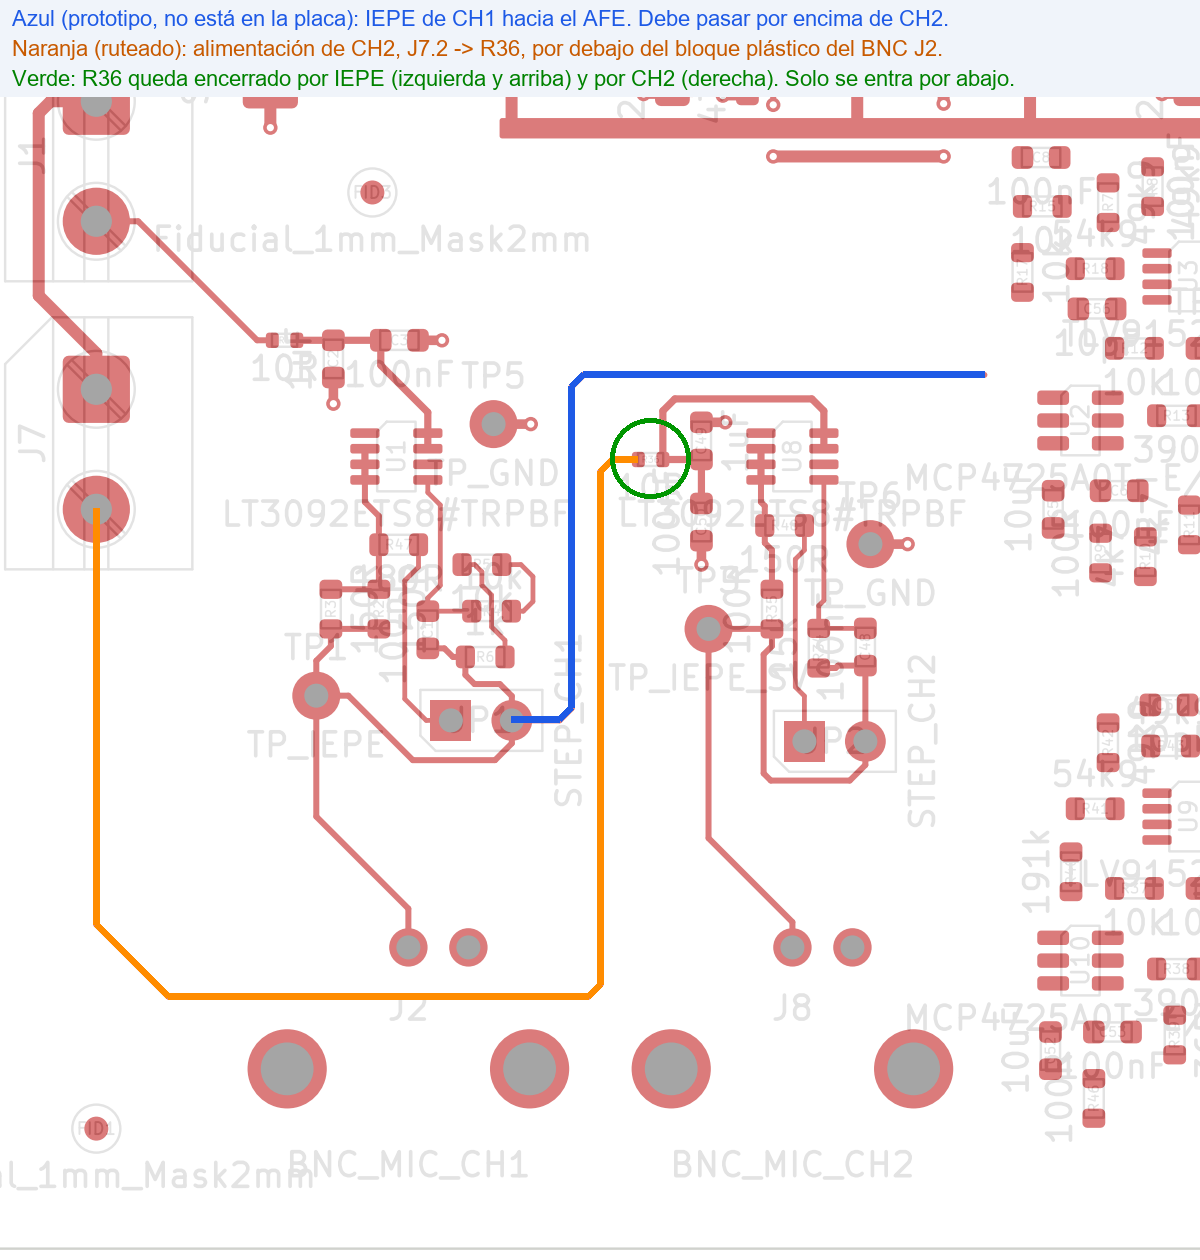
\includegraphics[width=0.75\linewidth]{figuras/bloque3_por_que_bajo_J2.png}
\caption{Bloque 3: por qué la alimentación del canal 2 tuvo que pasar bajo el cuerpo del BNC \net{J2} (prototipo en una
copia de la placa).}
\label{fig:c09-j2}
\end{figure}

\subsection{Bloque 4: el ADC PCM1808}

\begin{itemize}
  \item \textbf{AGND y DGND unidos debajo del integrado}, con una vía al plano, como pide el datasheet
  \doc{SLES177B §10.1.2}. Es el punto donde se tocan la tierra analógica y la digital del convertidor, y conviene que sea
  uno solo y debajo del chip.
  \item \textbf{Desacoplos con su vía:} \net{C17} (\SI{100}{\nano\farad} de VCC) quedó a \SI{0.71}{\milli\meter} del
  pin 3; \net{C11}$\leftrightarrow$\net{C12} y \net{C15}$\leftrightarrow$\net{C16} se intercambiaron para que el
  \SI{100}{\nano\farad} (el que actúa a alta frecuencia) quedara más cerca que el \SI{10}{\micro\farad}.
  \item \textbf{Straps:} \net{MD1} y \net{FMT} son niveles estáticos y quedaban encerrados en \capa{F.Cu} por las
  entradas analógicas; bajan a \capa{In2.Cu}. \net{MD0} pasa por debajo del cuerpo de \net{U4}.
  \item \textbf{Reloj lejos de lo analógico} (\SI{0.5}{\milli\meter}): \net{DOUT} pasa por debajo de \net{R19} gracias a
  que \net{R19} subió \SI{0.1}{\milli\meter}; la salida del oscilador entra a \net{R21} entre sus pads, porque el pad
  GND de \net{Y1} cierra el paso por la izquierda.
\end{itemize}

\subsection{Bloque 5: el AFE de los dos canales}

Es el bloque más delicado: aquí están el nodo \net{SUM}, la cadena de \SI{1}{\mega\ohm} y la realimentación. Todo en
\capa{F.Cu}.
\begin{itemize}
  \item \textbf{Cadena de entrada en columna:} \net{R13} $\to$ \net{R14} $\to$ \net{R16} vertical, y \net{R16.1}
  $\to$ \net{R18.2} pasando centrada entre los pads de \net{R17}.
  \item \textbf{Nodo \net{SUM} mínimo:} \net{R18.1} es el punto de unión; llegan \net{U3.2} (entrada inversora),
  \net{R7.1} (realimentación) y \net{C56.1} (el condensador CF). Cuanto más corto este nodo, menos capacidad parásita
  tiene y menos ruido capta (capítulo~\ref{cap:analog}).
  \item \textbf{La excepción del nodo \net{SUM}:} el enlace \net{C56.1} $\to$ \net{R18.1} no puede entrar por el eje de
  los dos pads con los quiebres fuera de ellos: los pads están a \SI{1.52}{\milli\meter} en $x$ y
  \SI{1.76}{\milli\meter} en $y$, con el otro pad de \net{C56} al lado. Se aceptó el enlace más corto
  (\SI{2.2}{\milli\meter}) con el quiebre a \ang{45} dentro del cobre de los pads. Igual en el canal 2
  (\net{C57.1}--\net{R41.1}).
  \item \textbf{\net{REST_OUT}} sale de \net{U3.1}, sube a \net{R8} y pasa por encima de \net{C7} hasta el punto de
  prueba \net{TP2}. No cabía entre \net{U3.8} y \net{C7} sin cortar el desacoplo; para abrir el paso \net{C7} bajó
  \SI{0.35}{\milli\meter} (queda a \SI{0.975}{\milli\meter} de \net{U3.8}).
  \item \textbf{Canal 2 igual al canal 1:} con la colocación original el canal 2 no salía limpio (el nodo
  \net{R39}--\net{R40} rodeaba el DAC \net{U10}). Se movieron \net{R38}/\net{R39}/\net{R40} a una columna, y \net{C57},
  \net{R43}, \net{TP4}, \net{C54}, \net{R44}, \net{R45} y \net{C55} a las posiciones equivalentes del canal 1. Ahora el
  canal 2 es el canal 1 desplazado \SI{22.5}{\milli\meter}.
\end{itemize}

\begin{figure}[htbp]
\centering
% generado por tikz_zona.py, ventana KiCad (138.5,116.5)-(158.5,139.5) mm, 0.62 cm/mm
\begin{tikzpicture}[line cap=round,line join=round]
\clip (0,0) rectangle (12.400,14.260);
\fill[fondo] (0,0) rectangle (12.400,14.260);
\fill[c24,opacity=0.35] (12.224,14.009) -- (12.232,14.006) -- (12.262,13.984) -- (12.262,13.984) -- (12.264,13.982) -- (12.276,13.946) -- (12.276,13.556) -- (12.273,13.537) -- (12.270,13.529) -- (12.248,13.499) -- (12.246,13.497) -- (12.210,13.485) -- (-10.593,13.485) -- (-10.612,13.488) -- (-10.620,13.491) -- (-10.650,13.513) -- (-10.650,13.513) -- (-10.652,13.515) -- (-10.664,13.551) -- (-10.664,13.941) -- (-10.661,13.960) -- (-10.658,13.968) -- (-10.636,13.998) -- (-10.636,13.999) -- (-10.634,14.000) -- (-10.598,14.012) -- (12.205,14.012) -- cycle;
\filldraw[fill=padfill,draw=paddraw,line width=0.2pt] (1.472,8.262) -- (1.520,8.252) -- (1.560,8.225) -- (1.587,8.185) -- (1.596,8.137) -- (1.596,7.889) -- (1.587,7.842) -- (1.560,7.802) -- (1.520,7.775) -- (1.472,7.766) -- (1.131,7.766) -- (1.084,7.775) -- (1.044,7.802) -- (1.017,7.842) -- (1.008,7.889) -- (1.008,8.137) -- (1.017,8.185) -- (1.044,8.225) -- (1.084,8.252) -- (1.131,8.262) -- cycle;
\filldraw[fill=padfill,draw=paddraw,line width=0.2pt] (1.472,7.238) -- (1.520,7.229) -- (1.560,7.202) -- (1.587,7.162) -- (1.596,7.114) -- (1.596,6.866) -- (1.587,6.819) -- (1.560,6.779) -- (1.520,6.752) -- (1.472,6.742) -- (1.131,6.742) -- (1.084,6.752) -- (1.044,6.779) -- (1.017,6.819) -- (1.008,6.866) -- (1.008,7.114) -- (1.017,7.162) -- (1.044,7.202) -- (1.084,7.229) -- (1.131,7.238) -- cycle;
\filldraw[fill=padfill,draw=paddraw,line width=0.2pt] (3.790,4.666) -- (3.843,4.655) -- (3.888,4.625) -- (3.919,4.579) -- (3.929,4.526) -- (3.929,4.247) -- (3.919,4.194) -- (3.888,4.148) -- (3.843,4.118) -- (3.790,4.108) -- (3.480,4.108) -- (3.426,4.118) -- (3.381,4.148) -- (3.351,4.194) -- (3.340,4.247) -- (3.340,4.526) -- (3.351,4.579) -- (3.381,4.625) -- (3.426,4.655) -- (3.480,4.666) -- cycle;
\filldraw[fill=padfill,draw=paddraw,line width=0.2pt] (3.790,3.705) -- (3.843,3.694) -- (3.888,3.664) -- (3.919,3.618) -- (3.929,3.565) -- (3.929,3.286) -- (3.919,3.233) -- (3.888,3.187) -- (3.843,3.157) -- (3.790,3.147) -- (3.480,3.147) -- (3.426,3.157) -- (3.381,3.187) -- (3.351,3.233) -- (3.340,3.286) -- (3.340,3.565) -- (3.351,3.618) -- (3.381,3.664) -- (3.426,3.694) -- (3.480,3.705) -- cycle;
\filldraw[fill=padfill,draw=paddraw,line width=0.2pt] (1.472,10.273) -- (1.520,10.263) -- (1.560,10.236) -- (1.587,10.196) -- (1.596,10.149) -- (1.596,9.901) -- (1.587,9.853) -- (1.560,9.813) -- (1.520,9.786) -- (1.472,9.777) -- (1.131,9.777) -- (1.084,9.786) -- (1.044,9.813) -- (1.017,9.853) -- (1.008,9.901) -- (1.008,10.149) -- (1.017,10.196) -- (1.044,10.236) -- (1.084,10.263) -- (1.131,10.273) -- cycle;
\filldraw[fill=padfill,draw=paddraw,line width=0.2pt] (1.472,9.250) -- (1.520,9.240) -- (1.560,9.213) -- (1.587,9.173) -- (1.596,9.126) -- (1.596,8.878) -- (1.587,8.830) -- (1.560,8.790) -- (1.520,8.763) -- (1.472,8.754) -- (1.131,8.754) -- (1.084,8.763) -- (1.044,8.790) -- (1.017,8.830) -- (1.008,8.878) -- (1.008,9.126) -- (1.017,9.173) -- (1.044,9.213) -- (1.084,9.240) -- (1.131,9.250) -- cycle;
\filldraw[fill=padfill,draw=paddraw,line width=0.2pt] (7.486,16.120) -- (7.546,16.108) -- (7.596,16.075) -- (7.630,16.024) -- (7.641,15.965) -- (7.641,15.655) -- (7.630,15.596) -- (7.596,15.545) -- (7.546,15.512) -- (7.486,15.500) -- (6.897,15.500) -- (6.838,15.512) -- (6.788,15.545) -- (6.754,15.596) -- (6.742,15.655) -- (6.742,15.965) -- (6.754,16.024) -- (6.788,16.075) -- (6.838,16.108) -- (6.897,16.120) -- cycle;
\filldraw[fill=padfill,draw=paddraw,line width=0.2pt] (7.486,14.942) -- (7.546,14.930) -- (7.596,14.897) -- (7.630,14.846) -- (7.641,14.787) -- (7.641,14.477) -- (7.630,14.418) -- (7.596,14.367) -- (7.546,14.334) -- (7.486,14.322) -- (6.897,14.322) -- (6.838,14.334) -- (6.788,14.367) -- (6.754,14.418) -- (6.742,14.477) -- (6.742,14.787) -- (6.754,14.846) -- (6.788,14.897) -- (6.838,14.930) -- (6.897,14.942) -- cycle;
\filldraw[fill=padfill,draw=paddraw,line width=0.2pt] (13.779,9.540) -- (13.732,9.550) -- (13.692,9.577) -- (13.665,9.617) -- (13.656,9.664) -- (13.656,9.912) -- (13.665,9.960) -- (13.692,10.000) -- (13.732,10.027) -- (13.779,10.036) -- (14.121,10.036) -- (14.168,10.027) -- (14.208,10.000) -- (14.235,9.960) -- (14.244,9.912) -- (14.244,9.664) -- (14.235,9.617) -- (14.208,9.577) -- (14.168,9.550) -- (14.121,9.540) -- cycle;
\filldraw[fill=padfill,draw=paddraw,line width=0.2pt] (13.779,10.563) -- (13.732,10.573) -- (13.692,10.600) -- (13.665,10.640) -- (13.656,10.687) -- (13.656,10.935) -- (13.665,10.983) -- (13.692,11.023) -- (13.732,11.050) -- (13.779,11.059) -- (14.121,11.059) -- (14.168,11.050) -- (14.208,11.023) -- (14.235,10.983) -- (14.244,10.935) -- (14.244,10.687) -- (14.235,10.640) -- (14.208,10.600) -- (14.168,10.573) -- (14.121,10.563) -- cycle;
\filldraw[fill=padfill,draw=paddraw,line width=0.2pt] (4.883,11.067) -- (4.835,11.076) -- (4.795,11.103) -- (4.768,11.144) -- (4.759,11.191) -- (4.759,11.439) -- (4.768,11.486) -- (4.795,11.527) -- (4.835,11.554) -- (4.883,11.563) -- (5.224,11.563) -- (5.271,11.554) -- (5.311,11.527) -- (5.338,11.486) -- (5.348,11.439) -- (5.348,11.191) -- (5.338,11.144) -- (5.311,11.103) -- (5.271,11.076) -- (5.224,11.067) -- cycle;
\filldraw[fill=padfill,draw=paddraw,line width=0.2pt] (4.883,12.090) -- (4.835,12.099) -- (4.795,12.126) -- (4.768,12.167) -- (4.759,12.214) -- (4.759,12.462) -- (4.768,12.509) -- (4.795,12.550) -- (4.835,12.577) -- (4.883,12.586) -- (5.224,12.586) -- (5.271,12.577) -- (5.311,12.550) -- (5.338,12.509) -- (5.348,12.462) -- (5.348,12.214) -- (5.338,12.167) -- (5.311,12.126) -- (5.271,12.099) -- (5.224,12.090) -- cycle;
\filldraw[fill=padfill,draw=paddraw,line width=0.2pt] (7.056,8.219) -- (7.067,8.272) -- (7.097,8.318) -- (7.142,8.348) -- (7.196,8.359) -- (7.475,8.359) -- (7.528,8.348) -- (7.574,8.318) -- (7.604,8.272) -- (7.614,8.219) -- (7.614,7.909) -- (7.604,7.856) -- (7.574,7.810) -- (7.528,7.780) -- (7.475,7.770) -- (7.196,7.770) -- (7.142,7.780) -- (7.097,7.810) -- (7.067,7.856) -- (7.056,7.909) -- cycle;
\filldraw[fill=padfill,draw=paddraw,line width=0.2pt] (8.017,8.219) -- (8.028,8.272) -- (8.058,8.318) -- (8.103,8.348) -- (8.157,8.359) -- (8.436,8.359) -- (8.489,8.348) -- (8.535,8.318) -- (8.565,8.272) -- (8.575,8.219) -- (8.575,7.909) -- (8.565,7.856) -- (8.535,7.810) -- (8.489,7.780) -- (8.436,7.770) -- (8.157,7.770) -- (8.103,7.780) -- (8.058,7.810) -- (8.028,7.856) -- (8.017,7.909) -- cycle;
\filldraw[fill=padfill,draw=paddraw,line width=0.2pt] (3.224,6.882) -- (3.231,6.918) -- (3.251,6.948) -- (3.281,6.968) -- (3.317,6.975) -- (3.953,6.975) -- (3.988,6.968) -- (4.018,6.948) -- (4.038,6.918) -- (4.046,6.882) -- (4.046,6.696) -- (4.038,6.660) -- (4.018,6.630) -- (3.988,6.610) -- (3.953,6.603) -- (3.317,6.603) -- (3.281,6.610) -- (3.251,6.630) -- (3.231,6.660) -- (3.224,6.696) -- cycle;
\filldraw[fill=padfill,draw=paddraw,line width=0.2pt] (3.224,6.293) -- (3.231,6.329) -- (3.251,6.359) -- (3.281,6.379) -- (3.317,6.386) -- (3.953,6.386) -- (3.988,6.379) -- (4.018,6.359) -- (4.038,6.329) -- (4.046,6.293) -- (4.046,6.107) -- (4.038,6.071) -- (4.018,6.041) -- (3.988,6.021) -- (3.953,6.014) -- (3.317,6.014) -- (3.281,6.021) -- (3.251,6.041) -- (3.231,6.071) -- (3.224,6.107) -- cycle;
\filldraw[fill=padfill,draw=paddraw,line width=0.2pt] (3.224,5.704) -- (3.231,5.740) -- (3.251,5.770) -- (3.281,5.790) -- (3.317,5.797) -- (3.953,5.797) -- (3.988,5.790) -- (4.018,5.770) -- (4.038,5.740) -- (4.046,5.704) -- (4.046,5.518) -- (4.038,5.482) -- (4.018,5.452) -- (3.988,5.432) -- (3.953,5.425) -- (3.317,5.425) -- (3.281,5.432) -- (3.251,5.452) -- (3.231,5.482) -- (3.224,5.518) -- cycle;
\filldraw[fill=padfill,draw=paddraw,line width=0.2pt] (4.634,5.704) -- (4.642,5.740) -- (4.662,5.770) -- (4.692,5.790) -- (4.728,5.797) -- (5.363,5.797) -- (5.399,5.790) -- (5.429,5.770) -- (5.449,5.740) -- (5.456,5.704) -- (5.456,5.518) -- (5.449,5.482) -- (5.429,5.452) -- (5.399,5.432) -- (5.363,5.425) -- (4.728,5.425) -- (4.692,5.432) -- (4.662,5.452) -- (4.642,5.482) -- (4.634,5.518) -- cycle;
\filldraw[fill=padfill,draw=paddraw,line width=0.2pt] (4.634,6.293) -- (4.642,6.329) -- (4.662,6.359) -- (4.692,6.379) -- (4.728,6.386) -- (5.363,6.386) -- (5.399,6.379) -- (5.429,6.359) -- (5.449,6.329) -- (5.456,6.293) -- (5.456,6.107) -- (5.449,6.071) -- (5.429,6.041) -- (5.399,6.021) -- (5.363,6.014) -- (4.728,6.014) -- (4.692,6.021) -- (4.662,6.041) -- (4.642,6.071) -- (4.634,6.107) -- cycle;
\filldraw[fill=padfill,draw=paddraw,line width=0.2pt] (4.634,6.882) -- (4.642,6.918) -- (4.662,6.948) -- (4.692,6.968) -- (4.728,6.975) -- (5.363,6.975) -- (5.399,6.968) -- (5.429,6.948) -- (5.449,6.918) -- (5.456,6.882) -- (5.456,6.696) -- (5.449,6.660) -- (5.429,6.630) -- (5.399,6.610) -- (5.363,6.603) -- (4.728,6.603) -- (4.692,6.610) -- (4.662,6.630) -- (4.642,6.660) -- (4.634,6.696) -- cycle;
\filldraw[fill=padfill,draw=paddraw,line width=0.2pt] (4.883,-1.860) -- (4.835,-1.851) -- (4.795,-1.824) -- (4.768,-1.783) -- (4.759,-1.736) -- (4.759,-1.488) -- (4.768,-1.441) -- (4.795,-1.400) -- (4.835,-1.373) -- (4.883,-1.364) -- (5.224,-1.364) -- (5.271,-1.373) -- (5.311,-1.400) -- (5.338,-1.441) -- (5.348,-1.488) -- (5.348,-1.736) -- (5.338,-1.783) -- (5.311,-1.824) -- (5.271,-1.851) -- (5.224,-1.860) -- cycle;
\filldraw[fill=padfill,draw=paddraw,line width=0.2pt] (4.976,8.235) -- (4.985,8.282) -- (5.012,8.322) -- (5.052,8.349) -- (5.099,8.359) -- (5.348,8.359) -- (5.395,8.349) -- (5.435,8.322) -- (5.462,8.282) -- (5.471,8.235) -- (5.471,7.894) -- (5.462,7.846) -- (5.435,7.806) -- (5.395,7.779) -- (5.348,7.770) -- (5.099,7.770) -- (5.052,7.779) -- (5.012,7.806) -- (4.985,7.846) -- (4.976,7.894) -- cycle;
\filldraw[fill=padfill,draw=paddraw,line width=0.2pt] (5.999,8.235) -- (6.008,8.282) -- (6.035,8.322) -- (6.075,8.349) -- (6.122,8.359) -- (6.371,8.359) -- (6.418,8.349) -- (6.458,8.322) -- (6.485,8.282) -- (6.494,8.235) -- (6.494,7.894) -- (6.485,7.846) -- (6.458,7.806) -- (6.418,7.779) -- (6.371,7.770) -- (6.122,7.770) -- (6.075,7.779) -- (6.035,7.806) -- (6.008,7.846) -- (5.999,7.894) -- cycle;
\filldraw[fill=padfill,draw=paddraw,line width=0.2pt] (10.305,10.585) -- (10.281,10.705) -- (10.235,10.817) -- (10.167,10.918) -- (10.081,11.004) -- (9.980,11.071) -- (9.868,11.118) -- (9.749,11.142) -- (9.627,11.142) -- (9.508,11.118) -- (9.396,11.071) -- (9.295,11.004) -- (9.209,10.918) -- (9.141,10.817) -- (9.095,10.705) -- (9.071,10.585) -- (9.071,10.464) -- (9.095,10.345) -- (9.141,10.232) -- (9.209,10.131) -- (9.295,10.045) -- (9.396,9.978) -- (9.508,9.931) -- (9.627,9.908) -- (9.749,9.908) -- (9.868,9.931) -- (9.980,9.978) -- (10.081,10.045) -- (10.167,10.131) -- (10.235,10.232) -- (10.281,10.345) -- (10.305,10.464) -- (10.305,10.585) -- cycle;
\fill[white] (9.688,10.525) circle (0.310);
\filldraw[fill=padfill,draw=paddraw,line width=0.2pt] (2.672,9.265) -- (2.624,9.275) -- (2.584,9.301) -- (2.557,9.342) -- (2.548,9.389) -- (2.548,9.637) -- (2.557,9.685) -- (2.584,9.725) -- (2.624,9.752) -- (2.672,9.761) -- (3.013,9.761) -- (3.060,9.752) -- (3.100,9.725) -- (3.127,9.685) -- (3.137,9.637) -- (3.137,9.389) -- (3.127,9.342) -- (3.100,9.301) -- (3.060,9.275) -- (3.013,9.265) -- cycle;
\filldraw[fill=padfill,draw=paddraw,line width=0.2pt] (2.672,10.288) -- (2.624,10.298) -- (2.584,10.324) -- (2.557,10.365) -- (2.548,10.412) -- (2.548,10.660) -- (2.557,10.708) -- (2.584,10.748) -- (2.624,10.775) -- (2.672,10.784) -- (3.013,10.784) -- (3.060,10.775) -- (3.100,10.748) -- (3.127,10.708) -- (3.137,10.660) -- (3.137,10.412) -- (3.127,10.365) -- (3.100,10.324) -- (3.060,10.298) -- (3.013,10.288) -- cycle;
\filldraw[fill=padfill,draw=paddraw,line width=0.2pt] (5.030,3.537) -- (5.077,3.527) -- (5.117,3.500) -- (5.144,3.460) -- (5.154,3.413) -- (5.154,3.165) -- (5.144,3.117) -- (5.117,3.077) -- (5.077,3.050) -- (5.030,3.041) -- (4.689,3.041) -- (4.641,3.050) -- (4.601,3.077) -- (4.574,3.117) -- (4.565,3.165) -- (4.565,3.413) -- (4.574,3.460) -- (4.601,3.500) -- (4.641,3.527) -- (4.689,3.537) -- cycle;
\filldraw[fill=padfill,draw=paddraw,line width=0.2pt] (5.030,2.514) -- (5.077,2.504) -- (5.117,2.477) -- (5.144,2.437) -- (5.154,2.390) -- (5.154,2.142) -- (5.144,2.094) -- (5.117,2.054) -- (5.077,2.027) -- (5.030,2.018) -- (4.689,2.018) -- (4.641,2.027) -- (4.601,2.054) -- (4.574,2.094) -- (4.565,2.142) -- (4.565,2.390) -- (4.574,2.437) -- (4.601,2.477) -- (4.641,2.504) -- (4.689,2.514) -- cycle;
\filldraw[fill=padfill,draw=paddraw,line width=0.2pt] (14.027,3.503) -- (14.017,3.450) -- (13.987,3.404) -- (13.941,3.374) -- (13.888,3.364) -- (13.609,3.364) -- (13.556,3.374) -- (13.510,3.404) -- (13.480,3.450) -- (13.469,3.503) -- (13.469,3.813) -- (13.480,3.866) -- (13.510,3.912) -- (13.556,3.942) -- (13.609,3.953) -- (13.888,3.953) -- (13.941,3.942) -- (13.987,3.912) -- (14.017,3.866) -- (14.027,3.813) -- cycle;
\filldraw[fill=padfill,draw=paddraw,line width=0.2pt] (6.033,-1.434) -- (5.986,-1.424) -- (5.946,-1.398) -- (5.919,-1.357) -- (5.909,-1.310) -- (5.909,-1.062) -- (5.919,-1.014) -- (5.946,-0.974) -- (5.986,-0.947) -- (6.033,-0.938) -- (6.374,-0.938) -- (6.422,-0.947) -- (6.462,-0.974) -- (6.489,-1.014) -- (6.498,-1.062) -- (6.498,-1.310) -- (6.489,-1.357) -- (6.462,-1.398) -- (6.422,-1.424) -- (6.374,-1.434) -- cycle;
\filldraw[fill=padfill,draw=paddraw,line width=0.2pt] (13.082,1.627) -- (13.135,1.617) -- (13.181,1.587) -- (13.211,1.541) -- (13.221,1.488) -- (13.221,1.209) -- (13.211,1.156) -- (13.181,1.110) -- (13.135,1.080) -- (13.082,1.069) -- (12.772,1.069) -- (12.719,1.080) -- (12.673,1.110) -- (12.643,1.156) -- (12.633,1.209) -- (12.633,1.488) -- (12.643,1.541) -- (12.673,1.587) -- (12.719,1.617) -- (12.772,1.627) -- cycle;
\filldraw[fill=padfill,draw=paddraw,line width=0.2pt] (13.082,0.666) -- (13.135,0.656) -- (13.181,0.626) -- (13.211,0.580) -- (13.221,0.527) -- (13.221,0.248) -- (13.211,0.195) -- (13.181,0.149) -- (13.135,0.119) -- (13.082,0.109) -- (12.772,0.109) -- (12.719,0.119) -- (12.673,0.149) -- (12.643,0.195) -- (12.633,0.248) -- (12.633,0.527) -- (12.643,0.580) -- (12.673,0.626) -- (12.719,0.656) -- (12.772,0.666) -- cycle;
\filldraw[fill=padfill,draw=paddraw,line width=0.2pt] (2.687,-0.705) -- (2.698,-0.652) -- (2.728,-0.607) -- (2.773,-0.576) -- (2.827,-0.566) -- (3.106,-0.566) -- (3.159,-0.576) -- (3.204,-0.607) -- (3.235,-0.652) -- (3.245,-0.705) -- (3.245,-1.015) -- (3.235,-1.069) -- (3.204,-1.114) -- (3.159,-1.144) -- (3.106,-1.155) -- (2.827,-1.155) -- (2.773,-1.144) -- (2.728,-1.114) -- (2.698,-1.069) -- (2.687,-1.015) -- cycle;
\filldraw[fill=padfill,draw=paddraw,line width=0.2pt] (3.648,-0.705) -- (3.659,-0.652) -- (3.689,-0.607) -- (3.734,-0.576) -- (3.788,-0.566) -- (4.067,-0.566) -- (4.120,-0.576) -- (4.165,-0.607) -- (4.196,-0.652) -- (4.206,-0.705) -- (4.206,-1.015) -- (4.196,-1.069) -- (4.165,-1.114) -- (4.120,-1.144) -- (4.067,-1.155) -- (3.788,-1.155) -- (3.734,-1.144) -- (3.689,-1.114) -- (3.659,-1.069) -- (3.648,-1.015) -- cycle;
\filldraw[fill=padfill,draw=paddraw,line width=0.2pt] (4.580,4.541) -- (4.591,4.595) -- (4.621,4.640) -- (4.666,4.670) -- (4.720,4.681) -- (4.999,4.681) -- (5.052,4.670) -- (5.097,4.640) -- (5.128,4.595) -- (5.138,4.541) -- (5.138,4.231) -- (5.128,4.178) -- (5.097,4.133) -- (5.052,4.103) -- (4.999,4.092) -- (4.720,4.092) -- (4.666,4.103) -- (4.621,4.133) -- (4.591,4.178) -- (4.580,4.231) -- cycle;
\filldraw[fill=padfill,draw=paddraw,line width=0.2pt] (5.541,4.541) -- (5.552,4.595) -- (5.582,4.640) -- (5.627,4.670) -- (5.681,4.681) -- (5.960,4.681) -- (6.013,4.670) -- (6.058,4.640) -- (6.089,4.595) -- (6.099,4.541) -- (6.099,4.231) -- (6.089,4.178) -- (6.058,4.133) -- (6.013,4.103) -- (5.960,4.092) -- (5.681,4.092) -- (5.627,4.103) -- (5.582,4.133) -- (5.552,4.178) -- (5.541,4.231) -- cycle;
\filldraw[fill=padfill,draw=paddraw,line width=0.2pt] (2.594,11.900) -- (2.604,11.948) -- (2.631,11.988) -- (2.671,12.015) -- (2.718,12.024) -- (2.966,12.024) -- (3.014,12.015) -- (3.054,11.988) -- (3.081,11.948) -- (3.090,11.900) -- (3.090,11.559) -- (3.081,11.512) -- (3.054,11.471) -- (3.014,11.445) -- (2.966,11.435) -- (2.718,11.435) -- (2.671,11.445) -- (2.631,11.471) -- (2.604,11.512) -- (2.594,11.559) -- cycle;
\filldraw[fill=padfill,draw=paddraw,line width=0.2pt] (3.617,11.900) -- (3.627,11.948) -- (3.654,11.988) -- (3.694,12.015) -- (3.741,12.024) -- (3.989,12.024) -- (4.037,12.015) -- (4.077,11.988) -- (4.104,11.948) -- (4.113,11.900) -- (4.113,11.559) -- (4.104,11.512) -- (4.077,11.471) -- (4.037,11.445) -- (3.989,11.435) -- (3.741,11.435) -- (3.694,11.445) -- (3.654,11.471) -- (3.627,11.512) -- (3.617,11.559) -- cycle;
\filldraw[fill=padfill,draw=paddraw,line width=0.2pt] (5.940,10.587) -- (5.944,10.610) -- (5.958,10.630) -- (5.978,10.644) -- (6.002,10.648) -- (6.634,10.648) -- (6.658,10.644) -- (6.678,10.630) -- (6.691,10.610) -- (6.696,10.587) -- (6.696,10.463) -- (6.691,10.439) -- (6.678,10.419) -- (6.658,10.405) -- (6.634,10.401) -- (6.002,10.401) -- (5.978,10.405) -- (5.958,10.419) -- (5.944,10.439) -- (5.940,10.463) -- cycle;
\filldraw[fill=padfill,draw=paddraw,line width=0.2pt] (5.940,10.183) -- (5.944,10.207) -- (5.958,10.227) -- (5.978,10.241) -- (6.002,10.246) -- (6.634,10.246) -- (6.658,10.241) -- (6.678,10.227) -- (6.691,10.207) -- (6.696,10.183) -- (6.696,10.059) -- (6.691,10.036) -- (6.678,10.016) -- (6.658,10.002) -- (6.634,9.998) -- (6.002,9.998) -- (5.978,10.002) -- (5.958,10.016) -- (5.944,10.036) -- (5.940,10.059) -- cycle;
\filldraw[fill=padfill,draw=paddraw,line width=0.2pt] (5.940,9.781) -- (5.944,9.804) -- (5.958,9.824) -- (5.978,9.838) -- (6.002,9.842) -- (6.634,9.842) -- (6.658,9.838) -- (6.678,9.824) -- (6.691,9.804) -- (6.696,9.781) -- (6.696,9.657) -- (6.691,9.633) -- (6.678,9.613) -- (6.658,9.599) -- (6.634,9.594) -- (6.002,9.594) -- (5.978,9.599) -- (5.958,9.613) -- (5.944,9.633) -- (5.940,9.657) -- cycle;
\filldraw[fill=padfill,draw=paddraw,line width=0.2pt] (5.940,9.377) -- (5.944,9.401) -- (5.958,9.421) -- (5.978,9.435) -- (6.002,9.439) -- (6.634,9.439) -- (6.658,9.435) -- (6.678,9.421) -- (6.691,9.401) -- (6.696,9.377) -- (6.696,9.253) -- (6.691,9.230) -- (6.678,9.210) -- (6.658,9.196) -- (6.634,9.192) -- (6.002,9.192) -- (5.978,9.196) -- (5.958,9.210) -- (5.944,9.230) -- (5.940,9.253) -- cycle;
\filldraw[fill=padfill,draw=paddraw,line width=0.2pt] (7.564,9.377) -- (7.569,9.401) -- (7.582,9.421) -- (7.602,9.435) -- (7.626,9.439) -- (8.258,9.439) -- (8.282,9.435) -- (8.302,9.421) -- (8.316,9.401) -- (8.320,9.377) -- (8.320,9.253) -- (8.316,9.230) -- (8.302,9.210) -- (8.282,9.196) -- (8.258,9.192) -- (7.626,9.192) -- (7.602,9.196) -- (7.582,9.210) -- (7.569,9.230) -- (7.564,9.253) -- cycle;
\filldraw[fill=padfill,draw=paddraw,line width=0.2pt] (7.564,9.781) -- (7.569,9.804) -- (7.582,9.824) -- (7.602,9.838) -- (7.626,9.842) -- (8.258,9.842) -- (8.282,9.838) -- (8.302,9.824) -- (8.316,9.804) -- (8.320,9.781) -- (8.320,9.657) -- (8.316,9.633) -- (8.302,9.613) -- (8.282,9.599) -- (8.258,9.594) -- (7.626,9.594) -- (7.602,9.599) -- (7.582,9.613) -- (7.569,9.633) -- (7.564,9.657) -- cycle;
\filldraw[fill=padfill,draw=paddraw,line width=0.2pt] (7.564,10.183) -- (7.569,10.207) -- (7.582,10.227) -- (7.602,10.241) -- (7.626,10.246) -- (8.258,10.246) -- (8.282,10.241) -- (8.302,10.227) -- (8.316,10.207) -- (8.320,10.183) -- (8.320,10.059) -- (8.316,10.036) -- (8.302,10.016) -- (8.282,10.002) -- (8.258,9.998) -- (7.626,9.998) -- (7.602,10.002) -- (7.582,10.016) -- (7.569,10.036) -- (7.564,10.059) -- cycle;
\filldraw[fill=padfill,draw=paddraw,line width=0.2pt] (7.564,10.587) -- (7.569,10.610) -- (7.582,10.630) -- (7.602,10.644) -- (7.626,10.648) -- (8.258,10.648) -- (8.282,10.644) -- (8.302,10.630) -- (8.316,10.610) -- (8.320,10.587) -- (8.320,10.463) -- (8.316,10.439) -- (8.302,10.419) -- (8.282,10.405) -- (8.258,10.401) -- (7.626,10.401) -- (7.602,10.405) -- (7.582,10.419) -- (7.569,10.439) -- (7.564,10.463) -- cycle;
\filldraw[fill=padfill,draw=paddraw,line width=0.2pt] (4.008,9.188) -- (4.019,9.242) -- (4.049,9.287) -- (4.094,9.317) -- (4.148,9.328) -- (4.427,9.328) -- (4.480,9.317) -- (4.525,9.287) -- (4.556,9.242) -- (4.566,9.188) -- (4.566,8.878) -- (4.556,8.825) -- (4.525,8.780) -- (4.480,8.750) -- (4.427,8.739) -- (4.148,8.739) -- (4.094,8.750) -- (4.049,8.780) -- (4.019,8.825) -- (4.008,8.878) -- cycle;
\filldraw[fill=padfill,draw=paddraw,line width=0.2pt] (4.969,9.188) -- (4.980,9.242) -- (5.010,9.287) -- (5.055,9.317) -- (5.109,9.328) -- (5.388,9.328) -- (5.441,9.317) -- (5.486,9.287) -- (5.517,9.242) -- (5.527,9.188) -- (5.527,8.878) -- (5.517,8.825) -- (5.486,8.780) -- (5.441,8.750) -- (5.388,8.739) -- (5.109,8.739) -- (5.055,8.750) -- (5.010,8.780) -- (4.980,8.825) -- (4.969,8.878) -- cycle;
\filldraw[fill=padfill,draw=paddraw,line width=0.2pt] (14.467,1.431) -- (14.456,1.377) -- (14.426,1.332) -- (14.380,1.302) -- (14.327,1.291) -- (14.048,1.291) -- (13.995,1.302) -- (13.949,1.332) -- (13.919,1.377) -- (13.909,1.431) -- (13.909,1.741) -- (13.919,1.794) -- (13.949,1.839) -- (13.995,1.870) -- (14.048,1.880) -- (14.327,1.880) -- (14.380,1.870) -- (14.426,1.839) -- (14.456,1.794) -- (14.467,1.741) -- cycle;
\filldraw[fill=padfill,draw=paddraw,line width=0.2pt] (6.033,11.481) -- (5.986,11.491) -- (5.946,11.518) -- (5.919,11.558) -- (5.909,11.605) -- (5.909,11.853) -- (5.919,11.901) -- (5.946,11.941) -- (5.986,11.968) -- (6.033,11.977) -- (6.374,11.977) -- (6.422,11.968) -- (6.462,11.941) -- (6.489,11.901) -- (6.498,11.853) -- (6.498,11.605) -- (6.489,11.558) -- (6.462,11.518) -- (6.422,11.491) -- (6.374,11.481) -- cycle;
\filldraw[fill=padfill,draw=paddraw,line width=0.2pt] (6.033,12.504) -- (5.986,12.514) -- (5.946,12.541) -- (5.919,12.581) -- (5.909,12.628) -- (5.909,12.876) -- (5.919,12.924) -- (5.946,12.964) -- (5.986,12.991) -- (6.033,13.000) -- (6.374,13.000) -- (6.422,12.991) -- (6.462,12.964) -- (6.489,12.924) -- (6.498,12.876) -- (6.498,12.628) -- (6.489,12.581) -- (6.462,12.541) -- (6.422,12.514) -- (6.374,12.504) -- cycle;
\filldraw[fill=padfill,draw=paddraw,line width=0.2pt] (7.990,-1.178) -- (8.044,-1.189) -- (8.089,-1.219) -- (8.119,-1.264) -- (8.130,-1.317) -- (8.130,-1.596) -- (8.119,-1.650) -- (8.089,-1.695) -- (8.044,-1.725) -- (7.990,-1.736) -- (7.680,-1.736) -- (7.627,-1.725) -- (7.582,-1.695) -- (7.551,-1.650) -- (7.541,-1.596) -- (7.541,-1.317) -- (7.551,-1.264) -- (7.582,-1.219) -- (7.627,-1.189) -- (7.680,-1.178) -- cycle;
\filldraw[fill=padfill,draw=paddraw,line width=0.2pt] (13.221,5.681) -- (13.168,5.691) -- (13.123,5.722) -- (13.092,5.767) -- (13.082,5.820) -- (13.082,6.099) -- (13.092,6.153) -- (13.123,6.198) -- (13.168,6.228) -- (13.221,6.239) -- (13.531,6.239) -- (13.585,6.228) -- (13.630,6.198) -- (13.660,6.153) -- (13.671,6.099) -- (13.671,5.820) -- (13.660,5.767) -- (13.630,5.722) -- (13.585,5.691) -- (13.531,5.681) -- cycle;
\filldraw[fill=padfill,draw=paddraw,line width=0.2pt] (13.221,6.642) -- (13.168,6.652) -- (13.123,6.683) -- (13.092,6.728) -- (13.082,6.781) -- (13.082,7.060) -- (13.092,7.114) -- (13.123,7.159) -- (13.168,7.189) -- (13.221,7.200) -- (13.531,7.200) -- (13.585,7.189) -- (13.630,7.159) -- (13.660,7.114) -- (13.671,7.060) -- (13.671,6.781) -- (13.660,6.728) -- (13.630,6.683) -- (13.585,6.652) -- (13.531,6.642) -- cycle;
\filldraw[fill=padfill,draw=paddraw,line width=0.2pt] (5.479,9.951) -- (5.470,9.904) -- (5.443,9.863) -- (5.403,9.836) -- (5.355,9.827) -- (5.107,9.827) -- (5.060,9.836) -- (5.020,9.863) -- (4.993,9.904) -- (4.983,9.951) -- (4.983,10.292) -- (4.993,10.339) -- (5.020,10.380) -- (5.060,10.407) -- (5.107,10.416) -- (5.355,10.416) -- (5.403,10.407) -- (5.443,10.380) -- (5.470,10.339) -- (5.479,10.292) -- cycle;
\filldraw[fill=padfill,draw=paddraw,line width=0.2pt] (4.456,9.951) -- (4.447,9.904) -- (4.420,9.863) -- (4.380,9.836) -- (4.332,9.827) -- (4.084,9.827) -- (4.037,9.836) -- (3.997,9.863) -- (3.970,9.904) -- (3.960,9.951) -- (3.960,10.292) -- (3.970,10.339) -- (3.997,10.380) -- (4.037,10.407) -- (4.084,10.416) -- (4.332,10.416) -- (4.380,10.407) -- (4.420,10.380) -- (4.447,10.339) -- (4.456,10.292) -- cycle;
\filldraw[fill=padfill,draw=paddraw,line width=0.2pt] (1.472,6.246) -- (1.520,6.237) -- (1.560,6.210) -- (1.587,6.170) -- (1.596,6.122) -- (1.596,5.874) -- (1.587,5.827) -- (1.560,5.787) -- (1.520,5.760) -- (1.472,5.751) -- (1.131,5.751) -- (1.084,5.760) -- (1.044,5.787) -- (1.017,5.827) -- (1.008,5.874) -- (1.008,6.122) -- (1.017,6.170) -- (1.044,6.210) -- (1.084,6.237) -- (1.131,6.246) -- cycle;
\filldraw[fill=padfill,draw=paddraw,line width=0.2pt] (1.472,5.224) -- (1.520,5.214) -- (1.560,5.187) -- (1.587,5.147) -- (1.596,5.099) -- (1.596,4.851) -- (1.587,4.804) -- (1.560,4.764) -- (1.520,4.737) -- (1.472,4.728) -- (1.131,4.728) -- (1.084,4.737) -- (1.044,4.764) -- (1.017,4.804) -- (1.008,4.851) -- (1.008,5.099) -- (1.017,5.147) -- (1.044,5.187) -- (1.084,5.214) -- (1.131,5.224) -- cycle;
\filldraw[fill=padfill,draw=paddraw,line width=0.2pt] (12.679,9.556) -- (12.726,9.546) -- (12.767,9.519) -- (12.794,9.479) -- (12.803,9.432) -- (12.803,9.184) -- (12.794,9.136) -- (12.767,9.096) -- (12.726,9.069) -- (12.679,9.060) -- (12.338,9.060) -- (12.291,9.069) -- (12.250,9.096) -- (12.223,9.136) -- (12.214,9.184) -- (12.214,9.432) -- (12.223,9.479) -- (12.250,9.519) -- (12.291,9.546) -- (12.338,9.556) -- cycle;
\filldraw[fill=padfill,draw=paddraw,line width=0.2pt] (12.679,8.533) -- (12.726,8.523) -- (12.767,8.496) -- (12.794,8.456) -- (12.803,8.409) -- (12.803,8.161) -- (12.794,8.113) -- (12.767,8.073) -- (12.726,8.046) -- (12.679,8.037) -- (12.338,8.037) -- (12.291,8.046) -- (12.250,8.073) -- (12.223,8.113) -- (12.214,8.161) -- (12.214,8.409) -- (12.223,8.456) -- (12.250,8.496) -- (12.291,8.523) -- (12.338,8.533) -- cycle;
\filldraw[fill=padfill,draw=paddraw,line width=0.2pt] (7.990,12.772) -- (8.044,12.761) -- (8.089,12.731) -- (8.119,12.686) -- (8.130,12.633) -- (8.130,12.353) -- (8.119,12.300) -- (8.089,12.255) -- (8.044,12.225) -- (7.990,12.214) -- (7.680,12.214) -- (7.627,12.225) -- (7.582,12.255) -- (7.551,12.300) -- (7.541,12.353) -- (7.541,12.633) -- (7.551,12.686) -- (7.582,12.731) -- (7.627,12.761) -- (7.680,12.772) -- cycle;
\filldraw[fill=padfill,draw=paddraw,line width=0.2pt] (7.990,11.811) -- (8.044,11.800) -- (8.089,11.770) -- (8.119,11.725) -- (8.130,11.672) -- (8.130,11.393) -- (8.119,11.339) -- (8.089,11.294) -- (8.044,11.264) -- (7.990,11.253) -- (7.680,11.253) -- (7.627,11.264) -- (7.582,11.294) -- (7.551,11.339) -- (7.541,11.393) -- (7.541,11.672) -- (7.551,11.725) -- (7.582,11.770) -- (7.627,11.800) -- (7.680,11.811) -- cycle;
\filldraw[fill=padfill,draw=paddraw,line width=0.2pt] (9.300,15.862) -- (9.347,15.852) -- (9.388,15.826) -- (9.415,15.785) -- (9.424,15.738) -- (9.424,15.490) -- (9.415,15.442) -- (9.388,15.402) -- (9.347,15.375) -- (9.300,15.366) -- (8.959,15.366) -- (8.912,15.375) -- (8.871,15.402) -- (8.844,15.442) -- (8.835,15.490) -- (8.835,15.738) -- (8.844,15.785) -- (8.871,15.826) -- (8.912,15.852) -- (8.959,15.862) -- cycle;
\filldraw[fill=padfill,draw=paddraw,line width=0.2pt] (9.300,14.839) -- (9.347,14.829) -- (9.388,14.803) -- (9.415,14.762) -- (9.424,14.715) -- (9.424,14.467) -- (9.415,14.419) -- (9.388,14.379) -- (9.347,14.352) -- (9.300,14.343) -- (8.959,14.343) -- (8.912,14.352) -- (8.871,14.379) -- (8.844,14.419) -- (8.835,14.467) -- (8.835,14.715) -- (8.844,14.762) -- (8.871,14.803) -- (8.912,14.829) -- (8.959,14.839) -- cycle;
\filldraw[fill=padfill,draw=paddraw,line width=0.2pt] (2.563,13.148) -- (2.574,13.201) -- (2.604,13.247) -- (2.649,13.277) -- (2.703,13.287) -- (2.982,13.287) -- (3.035,13.277) -- (3.080,13.247) -- (3.111,13.201) -- (3.121,13.148) -- (3.121,12.838) -- (3.111,12.784) -- (3.080,12.739) -- (3.035,12.709) -- (2.982,12.698) -- (2.703,12.698) -- (2.649,12.709) -- (2.604,12.739) -- (2.574,12.784) -- (2.563,12.838) -- cycle;
\filldraw[fill=padfill,draw=paddraw,line width=0.2pt] (3.524,13.148) -- (3.535,13.201) -- (3.565,13.247) -- (3.610,13.277) -- (3.664,13.287) -- (3.943,13.287) -- (3.996,13.277) -- (4.041,13.247) -- (4.072,13.201) -- (4.082,13.148) -- (4.082,12.838) -- (4.072,12.784) -- (4.041,12.739) -- (3.996,12.709) -- (3.943,12.698) -- (3.664,12.698) -- (3.610,12.709) -- (3.565,12.739) -- (3.535,12.784) -- (3.524,12.838) -- cycle;
\filldraw[fill=padfill,draw=paddraw,line width=0.2pt] (-1.061,1.110) -- (-1.008,1.099) -- (-0.962,1.069) -- (-0.932,1.023) -- (-0.921,0.970) -- (-0.921,0.691) -- (-0.932,0.638) -- (-0.962,0.592) -- (-1.008,0.562) -- (-1.061,0.552) -- (-1.371,0.552) -- (-1.424,0.562) -- (-1.470,0.592) -- (-1.500,0.638) -- (-1.510,0.691) -- (-1.510,0.970) -- (-1.500,1.023) -- (-1.470,1.069) -- (-1.424,1.099) -- (-1.371,1.110) -- cycle;
\filldraw[fill=padfill,draw=paddraw,line width=0.2pt] (-1.061,0.149) -- (-1.008,0.138) -- (-0.962,0.108) -- (-0.932,0.062) -- (-0.921,0.009) -- (-0.921,-0.270) -- (-0.932,-0.323) -- (-0.962,-0.369) -- (-1.008,-0.399) -- (-1.061,-0.409) -- (-1.371,-0.409) -- (-1.424,-0.399) -- (-1.470,-0.369) -- (-1.500,-0.323) -- (-1.510,-0.270) -- (-1.510,0.009) -- (-1.500,0.062) -- (-1.470,0.108) -- (-1.424,0.138) -- (-1.371,0.149) -- cycle;
\filldraw[fill=padfill,draw=paddraw,line width=0.2pt] (12.664,11.577) -- (12.717,11.566) -- (12.762,11.536) -- (12.792,11.491) -- (12.803,11.437) -- (12.803,11.158) -- (12.792,11.105) -- (12.762,11.060) -- (12.717,11.030) -- (12.664,11.019) -- (12.354,11.019) -- (12.300,11.030) -- (12.255,11.060) -- (12.225,11.105) -- (12.214,11.158) -- (12.214,11.437) -- (12.225,11.491) -- (12.255,11.536) -- (12.300,11.566) -- (12.354,11.577) -- cycle;
\filldraw[fill=padfill,draw=paddraw,line width=0.2pt] (12.664,10.616) -- (12.717,10.605) -- (12.762,10.575) -- (12.792,10.530) -- (12.803,10.476) -- (12.803,10.197) -- (12.792,10.144) -- (12.762,10.099) -- (12.717,10.069) -- (12.664,10.058) -- (12.354,10.058) -- (12.300,10.069) -- (12.255,10.099) -- (12.225,10.144) -- (12.214,10.197) -- (12.214,10.476) -- (12.225,10.530) -- (12.255,10.575) -- (12.300,10.605) -- (12.354,10.616) -- cycle;
\filldraw[fill=padfill,draw=paddraw,line width=0.2pt] (7.324,4.264) -- (7.371,4.254) -- (7.411,4.227) -- (7.438,4.187) -- (7.448,4.140) -- (7.448,3.892) -- (7.438,3.844) -- (7.411,3.804) -- (7.371,3.777) -- (7.324,3.768) -- (6.983,3.768) -- (6.935,3.777) -- (6.895,3.804) -- (6.868,3.844) -- (6.859,3.892) -- (6.859,4.140) -- (6.868,4.187) -- (6.895,4.227) -- (6.935,4.254) -- (6.983,4.264) -- cycle;
\filldraw[fill=padfill,draw=paddraw,line width=0.2pt] (7.324,3.241) -- (7.371,3.231) -- (7.411,3.204) -- (7.438,3.164) -- (7.448,3.117) -- (7.448,2.869) -- (7.438,2.821) -- (7.411,2.781) -- (7.371,2.754) -- (7.324,2.745) -- (6.983,2.745) -- (6.935,2.754) -- (6.895,2.781) -- (6.868,2.821) -- (6.859,2.869) -- (6.859,3.117) -- (6.868,3.164) -- (6.895,3.204) -- (6.935,3.231) -- (6.983,3.241) -- cycle;
\filldraw[fill=padfill,draw=paddraw,line width=0.2pt] (6.187,3.442) -- (6.235,3.433) -- (6.275,3.406) -- (6.302,3.366) -- (6.311,3.318) -- (6.311,3.070) -- (6.302,3.023) -- (6.275,2.983) -- (6.235,2.956) -- (6.187,2.946) -- (5.846,2.946) -- (5.799,2.956) -- (5.758,2.983) -- (5.732,3.023) -- (5.722,3.070) -- (5.722,3.318) -- (5.732,3.366) -- (5.758,3.406) -- (5.799,3.433) -- (5.846,3.442) -- cycle;
\filldraw[fill=padfill,draw=paddraw,line width=0.2pt] (6.187,2.419) -- (6.235,2.410) -- (6.275,2.383) -- (6.302,2.343) -- (6.311,2.295) -- (6.311,2.047) -- (6.302,2.000) -- (6.275,1.960) -- (6.235,1.933) -- (6.187,1.923) -- (5.846,1.923) -- (5.799,1.933) -- (5.758,1.960) -- (5.732,2.000) -- (5.722,2.047) -- (5.722,2.295) -- (5.732,2.343) -- (5.758,2.383) -- (5.799,2.410) -- (5.846,2.419) -- cycle;
\filldraw[fill=padfill,draw=paddraw,line width=0.2pt] (13.656,4.580) -- (13.645,4.527) -- (13.615,4.482) -- (13.569,4.451) -- (13.516,4.441) -- (13.237,4.441) -- (13.184,4.451) -- (13.138,4.482) -- (13.108,4.527) -- (13.098,4.580) -- (13.098,4.890) -- (13.108,4.944) -- (13.138,4.989) -- (13.184,5.019) -- (13.237,5.030) -- (13.516,5.030) -- (13.569,5.019) -- (13.615,4.989) -- (13.645,4.944) -- (13.656,4.890) -- cycle;
\filldraw[fill=padfill,draw=paddraw,line width=0.2pt] (12.694,4.580) -- (12.684,4.527) -- (12.654,4.482) -- (12.608,4.451) -- (12.555,4.441) -- (12.276,4.441) -- (12.223,4.451) -- (12.177,4.482) -- (12.147,4.527) -- (12.136,4.580) -- (12.136,4.890) -- (12.147,4.944) -- (12.177,4.989) -- (12.223,5.019) -- (12.276,5.030) -- (12.555,5.030) -- (12.608,5.019) -- (12.654,4.989) -- (12.684,4.944) -- (12.694,4.890) -- cycle;
\filldraw[fill=padfill,draw=paddraw,line width=0.2pt] (-0.468,3.068) -- (-0.492,3.187) -- (-0.538,3.299) -- (-0.606,3.400) -- (-0.692,3.486) -- (-0.793,3.554) -- (-0.905,3.600) -- (-1.024,3.624) -- (-1.146,3.624) -- (-1.265,3.600) -- (-1.377,3.554) -- (-1.478,3.486) -- (-1.564,3.400) -- (-1.632,3.299) -- (-1.678,3.187) -- (-1.702,3.068) -- (-1.702,2.946) -- (-1.678,2.827) -- (-1.632,2.715) -- (-1.564,2.614) -- (-1.478,2.528) -- (-1.377,2.460) -- (-1.265,2.414) -- (-1.146,2.390) -- (-1.024,2.390) -- (-0.905,2.414) -- (-0.793,2.460) -- (-0.692,2.528) -- (-0.606,2.614) -- (-0.538,2.715) -- (-0.492,2.827) -- (-0.468,2.946) -- (-0.468,3.068) -- cycle;
\fill[white] (-1.085,3.007) circle (0.310);
\filldraw[fill=padfill,draw=paddraw,line width=0.2pt] (13.411,8.111) -- (13.377,8.118) -- (13.349,8.137) -- (13.330,8.165) -- (13.324,8.198) -- (13.324,8.372) -- (13.330,8.405) -- (13.349,8.433) -- (13.377,8.452) -- (13.411,8.458) -- (13.621,8.458) -- (13.655,8.452) -- (13.683,8.433) -- (13.702,8.405) -- (13.708,8.372) -- (13.708,8.198) -- (13.702,8.165) -- (13.683,8.137) -- (13.655,8.118) -- (13.621,8.111) -- cycle;
\filldraw[fill=padfill,draw=paddraw,line width=0.2pt] (13.411,8.706) -- (13.377,8.713) -- (13.349,8.732) -- (13.330,8.760) -- (13.324,8.793) -- (13.324,8.967) -- (13.330,9.000) -- (13.349,9.028) -- (13.377,9.047) -- (13.411,9.054) -- (13.621,9.054) -- (13.655,9.047) -- (13.683,9.028) -- (13.702,9.000) -- (13.708,8.967) -- (13.708,8.793) -- (13.702,8.760) -- (13.683,8.732) -- (13.655,8.713) -- (13.621,8.706) -- cycle;
\draw[cB,line width=0.310cm,densely dashed] (0.806,14.384) -- (0.806,13.020);
\draw[cB,line width=0.186cm,densely dashed] (9.827,13.020) -- (9.827,14.353);
\draw[cB,line width=0.124cm,densely dashed] (12.214,0.837) -- (12.214,-2.666);
\draw[cB,line width=0.124cm,densely dashed] (11.842,1.209) -- (12.214,0.837);
\draw[cB,line width=0.124cm,densely dashed] (7.874,1.581) -- (8.246,1.209);
\draw[cB,line width=0.124cm,densely dashed] (7.874,4.016) -- (7.874,1.581);
\draw[cB,line width=0.124cm,densely dashed] (8.246,1.209) -- (11.842,1.209);
\draw[cB,line width=0.124cm,densely dashed] (6.262,6.200) -- (6.262,2.313);
\draw[cB,line width=0.124cm,densely dashed] (5.437,1.209) -- (5.809,0.837);
\draw[cB,line width=0.124cm,densely dashed] (11.470,0.837) -- (11.842,0.465);
\draw[cB,line width=0.124cm,densely dashed] (6.262,2.313) -- (5.437,1.488);
\draw[cB,line width=0.124cm,densely dashed] (11.842,0.465) -- (11.842,-3.038);
\draw[cB,line width=0.124cm,densely dashed] (5.809,0.837) -- (11.470,0.837);
\draw[cB,line width=0.124cm,densely dashed] (5.437,1.488) -- (5.437,1.209);
\draw[cB,line width=0.124cm,densely dashed] (10.664,-0.682) -- (10.664,-4.185);
\draw[cB,line width=0.124cm,densely dashed] (2.294,-2.124) -- (2.294,-0.682);
\draw[cB,line width=0.124cm,densely dashed] (2.666,-0.310) -- (10.292,-0.310);
\draw[cB,line width=0.124cm,densely dashed] (2.294,-0.682) -- (2.666,-0.310);
\draw[cB,line width=0.124cm,densely dashed] (10.292,-0.310) -- (10.664,-0.682);
\draw[cB,line width=0.124cm,densely dashed] (0.558,11.420) -- (0.558,0.434);
\draw[cB,line width=0.124cm,densely dashed] (0.558,0.434) -- (0.930,0.062);
\draw[cB,line width=0.124cm,densely dashed] (1.984,11.730) -- (0.868,11.730);
\draw[cB,line width=0.124cm,densely dashed] (11.036,-0.310) -- (11.036,-3.813);
\draw[cB,line width=0.124cm,densely dashed] (0.930,0.062) -- (10.664,0.062);
\draw[cB,line width=0.124cm,densely dashed] (0.868,11.730) -- (0.558,11.420);
\draw[cB,line width=0.124cm,densely dashed] (10.664,0.062) -- (11.036,-0.310);
\draw[cIn,line width=0.248cm,densely dashed] (4.859,1.600) -- (4.859,1.271);
\draw[cIn,line width=0.248cm,densely dashed] (6.017,1.274) -- (6.017,1.507);
\draw[cIn,line width=0.248cm,densely dashed] (0.558,12.772) -- (0.558,3.162);
\draw[cIn,line width=0.248cm,densely dashed] (0.806,15.438) -- (1.178,15.810);
\draw[cIn,line width=0.248cm,densely dashed] (0.806,13.020) -- (0.558,12.772);
\draw[cIn,line width=0.248cm,densely dashed] (4.030,1.922) -- (3.410,1.302);
\draw[cIn,line width=0.248cm,densely dashed] (4.859,1.271) -- (5.107,1.023);
\draw[cIn,line width=0.248cm,densely dashed] (0.558,3.162) -- (0.930,2.790);
\draw[cIn,line width=0.248cm,densely dashed] (4.030,2.266) -- (4.030,1.922);
\draw[cIn,line width=0.248cm,densely dashed] (0.930,2.790) -- (3.506,2.790);
\draw[cIn,line width=0.248cm,densely dashed] (1.736,1.302) -- (1.364,0.930);
\draw[cIn,line width=0.248cm,densely dashed] (5.107,1.023) -- (5.766,1.023);
\draw[cIn,line width=0.248cm,densely dashed] (1.364,0.930) -- (1.364,-12.115);
\draw[cIn,line width=0.248cm,densely dashed] (5.766,1.023) -- (6.017,1.274);
\draw[cIn,line width=0.248cm,densely dashed] (3.506,2.790) -- (4.030,2.266);
\draw[cIn,line width=0.248cm,densely dashed] (3.410,1.302) -- (1.736,1.302);
\draw[cIn,line width=0.248cm,densely dashed] (0.806,14.384) -- (0.806,15.438);
\draw[cIn,line width=0.124cm,densely dashed] (15.810,6.820) -- (13.206,6.820);
\draw[cIn,line width=0.124cm,densely dashed] (13.206,6.820) -- (12.896,7.130);
\draw[cIn,line width=0.124cm,densely dashed] (12.896,7.130) -- (12.896,9.431);
\draw[cIn,line width=0.124cm,densely dashed] (12.896,9.431) -- (13.252,9.788);
\draw[cIn,line width=0.248cm,densely dashed] (7.750,13.330) -- (7.750,11.904);
\draw[cIn,line width=0.248cm,densely dashed] (7.750,11.904) -- (8.122,11.532);
\draw[cIn,line width=0.248cm,densely dashed] (8.122,13.702) -- (7.750,13.330);
\draw[cIn,line width=0.248cm,densely dashed] (10.850,-0.031) -- (10.850,-1.984);
\draw[cIn,line width=0.248cm,densely dashed] (8.122,11.532) -- (8.544,11.532);
\draw[cIn,line width=0.248cm,densely dashed] (14.043,2.046) -- (12.927,2.046);
\draw[cIn,line width=0.248cm,densely dashed] (15.500,13.702) -- (8.122,13.702);
\draw[cIn,line width=0.248cm,densely dashed] (12.927,2.046) -- (10.850,-0.031);
\draw[cSig,line width=0.124cm] (7.018,-1.948) -- (7.018,-0.992);
\draw[cSig,line width=0.124cm] (11.160,-2.681) -- (11.160,10.740);
\draw[cSig,line width=0.124cm] (7.018,-0.992) -- (7.273,-0.738);
\draw[cSig,line width=0.124cm] (11.718,11.298) -- (12.509,11.298);
\draw[cSig,line width=0.124cm] (9.021,-0.986) -- (9.021,-2.061);
\draw[cSig,line width=0.124cm] (11.160,10.740) -- (11.718,11.298);
\draw[cSig,line width=0.124cm] (8.773,-0.738) -- (9.021,-0.986);
\draw[cSig,line width=0.124cm] (7.273,-0.738) -- (8.773,-0.738);
\draw[cSig,line width=0.124cm] (1.302,8.013) -- (1.302,9.002);
\draw[cSig,line width=0.124cm] (1.302,5.999) -- (1.302,6.991);
\draw[cSig,line width=0.186cm] (4.859,4.386) -- (4.859,3.289);
\draw[cSig,line width=0.186cm] (3.635,4.386) -- (4.859,4.386);
\draw[cSig,line width=0.186cm] (3.635,5.611) -- (3.635,4.386);
\draw[cGND,line width=0.248cm] (3.927,-0.860) -- (4.619,-0.860);
\draw[cGND,line width=0.248cm] (7.192,14.632) -- (6.324,14.632);
\draw[cGND,line width=0.248cm] (3.635,3.426) -- (2.933,3.426);
\draw[cGND,line width=0.155cm] (7.719,14.632) -- (7.192,14.632);
\draw[cGND,line width=0.248cm] (2.842,9.513) -- (2.842,8.854);
\draw[cGND,line width=0.155cm] (8.029,14.942) -- (7.719,14.632);
\draw[cGND,line width=0.248cm] (12.927,0.388) -- (12.927,-0.294);
\draw[cGND,line width=0.248cm] (8.296,8.064) -- (8.296,8.767);
\draw[cGND,line width=0.248cm] (3.803,12.993) -- (4.495,12.993);
\draw[cGND,line width=0.248cm] (13.749,3.658) -- (13.051,3.658);
\draw[cGND,line width=0.248cm] (7.835,12.493) -- (8.544,12.493);
\draw[cGND,line width=0.248cm] (-1.085,3.007) -- (-0.062,3.007);
\draw[cGND,line width=0.248cm] (12.416,4.735) -- (11.734,4.735);
\draw[cGND,line width=0.186cm] (3.635,6.200) -- (2.821,6.200);
\draw[cGND,line width=0.186cm] (5.045,6.789) -- (5.859,6.789);
\draw[cGND,line width=0.248cm] (5.820,4.386) -- (5.820,5.090);
\draw[cGND,line width=0.248cm] (9.129,14.591) -- (8.432,14.591);
\draw[cGND,line width=0.248cm] (14.308,2.677) -- (13.626,2.677);
\draw[cGND,line width=0.248cm] (13.376,6.920) -- (13.376,7.609);
\draw[cGND,line width=0.186cm] (6.318,9.316) -- (6.318,8.785);
\draw[cGND,line width=0.155cm] (8.029,16.895) -- (8.029,14.942);
\draw[cOut,line width=0.186cm] (4.859,2.266) -- (4.859,1.600);
\draw[cOut,line width=0.186cm] (6.017,2.171) -- (6.696,2.171);
\draw[cOut,line width=0.186cm] (6.696,2.171) -- (7.153,2.629);
\draw[cOut,line width=0.186cm] (7.153,2.629) -- (7.153,2.993);
\draw[cOut,line width=0.186cm] (6.017,2.171) -- (6.017,1.507);
\draw[cOut,line width=0.186cm] (4.859,2.266) -- (4.030,2.266);
\draw[cOut,line width=0.310cm] (0.806,13.020) -- (-3.565,13.020);
\draw[cOut,line width=0.310cm] (0.806,22.801) -- (0.806,14.384);
\draw[cSig,line width=0.124cm] (-2.421,0.831) -- (-1.216,0.831);
\draw[cSig,line width=0.124cm] (3.507,10.122) -- (4.208,10.122);
\draw[cSig,line width=0.124cm] (1.302,10.025) -- (3.410,10.025);
\draw[cSig,line width=0.124cm] (3.410,10.025) -- (3.507,10.122);
\draw[cSig,line width=0.155cm] (-1.906,7.440) -- (0.558,4.976);
\draw[cSig,line width=0.155cm] (0.558,4.976) -- (1.302,4.976);
\draw[c24,line width=0.310cm] (3.038,17.081) -- (3.038,13.764);
\draw[c24,line width=0.310cm] (11.966,17.081) -- (11.966,13.764);
\draw[cSig,line width=0.124cm] (13.252,9.788) -- (13.950,9.788);
\draw[cSig,line width=0.124cm] (4.287,9.105) -- (5.231,10.049);
\draw[cSig,line width=0.124cm] (5.053,10.912) -- (5.231,10.734);
\draw[cSig,line width=0.124cm] (5.231,10.122) -- (6.318,10.122);
\draw[cSig,line width=0.124cm] (4.287,9.033) -- (4.287,9.105);
\draw[cSig,line width=0.124cm] (5.231,10.734) -- (5.231,10.122);
\draw[cSig,line width=0.124cm] (5.231,10.049) -- (5.231,10.122);
\draw[cSig,line width=0.124cm] (5.053,11.315) -- (5.053,10.912);
\draw[cSig,line width=0.124cm] (5.870,12.752) -- (6.204,12.752);
\draw[cSig,line width=0.124cm] (5.456,12.338) -- (5.870,12.752);
\draw[cSig,line width=0.124cm] (5.053,12.338) -- (5.456,12.338);
\draw[cSig,line width=0.124cm] (7.273,13.212) -- (8.773,13.212);
\draw[cSig,line width=0.124cm] (9.021,11.889) -- (9.688,11.222);
\draw[cSig,line width=0.124cm] (4.313,11.827) -- (4.216,11.730);
\draw[cSig,line width=0.124cm] (9.688,11.222) -- (9.688,10.525);
\draw[cSig,line width=0.124cm] (5.248,9.033) -- (5.580,9.033);
\draw[cSig,line width=0.124cm] (8.897,7.502) -- (9.688,8.293);
\draw[cSig,line width=0.124cm] (8.773,13.212) -- (9.021,12.964);
\draw[cSig,line width=0.124cm] (6.204,11.729) -- (6.758,11.729);
\draw[cSig,line width=0.124cm] (6.318,11.098) -- (6.204,11.212);
\draw[cSig,line width=0.124cm] (7.018,12.958) -- (7.273,13.212);
\draw[cSig,line width=0.124cm] (5.580,9.033) -- (5.735,8.878);
\draw[cSig,line width=0.124cm] (7.018,11.990) -- (7.018,12.958);
\draw[cSig,line width=0.124cm] (6.758,11.729) -- (7.018,11.990);
\draw[cSig,line width=0.124cm] (6.318,10.524) -- (6.318,11.098);
\draw[cSig,line width=0.124cm] (9.688,8.293) -- (9.688,10.525);
\draw[cSig,line width=0.124cm] (10.416,10.525) -- (12.539,12.648);
\draw[cSig,line width=0.124cm] (12.539,12.648) -- (14.074,12.648);
\draw[cSig,line width=0.124cm] (5.890,7.502) -- (8.897,7.502);
\draw[cSig,line width=0.124cm] (6.204,11.212) -- (6.204,11.729);
\draw[cSig,line width=0.124cm] (5.793,11.827) -- (4.313,11.827);
\draw[cSig,line width=0.124cm] (5.735,8.878) -- (5.735,7.657);
\draw[cSig,line width=0.124cm] (5.735,7.657) -- (5.890,7.502);
\draw[cSig,line width=0.124cm] (6.204,11.729) -- (5.890,11.729);
\draw[cSig,line width=0.124cm] (9.688,10.525) -- (10.416,10.525);
\draw[cSig,line width=0.124cm] (9.021,12.964) -- (9.021,11.889);
\draw[cSig,line width=0.124cm] (4.216,11.730) -- (3.865,11.730);
\draw[cSig,line width=0.124cm] (5.890,11.729) -- (5.793,11.827);
\draw[cSig,line width=0.124cm] (7.335,8.445) -- (7.335,8.064);
\draw[cSig,line width=0.124cm] (7.942,9.316) -- (7.942,9.052);
\draw[cSig,line width=0.124cm] (6.246,8.064) -- (7.335,8.064);
\draw[cSig,line width=0.124cm] (7.942,9.052) -- (7.335,8.445);
\draw[cOut,line width=0.155cm] (13.811,13.020) -- (9.827,13.020);
\draw[cOut,line width=0.155cm] (9.827,14.353) -- (9.827,17.495);
\draw[cSig,line width=0.124cm] (3.635,6.789) -- (3.635,7.192);
\draw[cSig,line width=0.124cm] (3.635,7.192) -- (4.507,8.064);
\draw[cSig,line width=0.124cm] (4.507,8.064) -- (5.224,8.064);
\draw[cSig,line width=0.124cm] (7.153,5.340) -- (7.153,4.016);
\draw[cSig,line width=0.124cm] (5.045,5.611) -- (6.882,5.611);
\draw[cSig,line width=0.124cm] (7.153,4.016) -- (7.874,4.016);
\draw[cSig,line width=0.124cm] (6.882,5.611) -- (7.153,5.340);
\draw[cSig,line width=0.124cm] (5.437,2.990) -- (5.437,1.488);
\draw[cSig,line width=0.124cm] (6.017,3.194) -- (5.642,3.194);
\draw[cSig,line width=0.124cm] (5.642,3.194) -- (5.437,2.990);
\draw[cSig,line width=0.124cm] (5.045,6.200) -- (6.262,6.200);
\draw[cSig,line width=0.124cm] (5.456,-1.612) -- (5.882,-1.186);
\draw[cSig,line width=0.124cm] (5.882,-1.186) -- (6.204,-1.186);
\draw[cSig,line width=0.124cm] (2.966,-2.124) -- (2.966,-0.860);
\draw[cSig,line width=0.124cm] (2.842,11.730) -- (2.842,10.536);
\draw[cSig,line width=0.124cm] (2.842,11.730) -- (2.842,12.993);
\draw[cSig,line width=0.124cm] (2.842,11.730) -- (1.984,11.730);
\draw[cOut,line width=0.186cm] (7.942,10.524) -- (7.942,10.912);
\draw[cOut,line width=0.186cm] (7.835,11.019) -- (7.835,11.532);
\draw[cOut,line width=0.186cm] (7.835,11.532) -- (8.544,11.532);
\draw[cOut,line width=0.186cm] (12.927,1.349) -- (12.927,2.046);
\draw[cOut,line width=0.186cm] (7.942,10.912) -- (7.835,11.019);
\draw[cSig,line width=0.124cm] (7.942,10.122) -- (7.942,9.718);
\draw[cSig,line width=0.124cm] (6.318,9.718) -- (7.942,9.718);
\draw[cSig,line width=0.155cm] (-1.922,-0.130) -- (-1.216,-0.130);
\draw[cSig,line width=0.155cm] (-1.216,-0.130) -- (-1.216,-2.087);
\draw[cSig,line width=0.155cm] (13.376,4.735) -- (13.376,5.960);
\draw[cSig,line width=0.155cm] (14.601,4.735) -- (13.376,4.735);
\draw[cSig,line width=0.155cm] (12.509,9.308) -- (12.509,10.337);
\draw[cSig,line width=0.155cm] (13.516,8.284) -- (12.509,8.284);
\draw[cSig,line width=0.155cm] (14.601,8.284) -- (13.516,8.284);
\filldraw[fill=cGND,draw=black,line width=0.2pt] (3.782,10.788) circle (0.186);
\fill[white] (3.782,10.788) circle (0.093);
\filldraw[fill=cGND,draw=black,line width=0.2pt] (2.842,8.854) circle (0.186);
\fill[white] (2.842,8.854) circle (0.093);
\filldraw[fill=cGND,draw=black,line width=0.2pt] (2.232,12.338) circle (0.186);
\fill[white] (2.232,12.338) circle (0.093);
\filldraw[fill=cGND,draw=black,line width=0.2pt] (2.232,8.990) circle (0.186);
\fill[white] (2.232,8.990) circle (0.093);
\filldraw[fill=cGND,draw=black,line width=0.2pt] (11.734,4.735) circle (0.186);
\fill[white] (11.734,4.735) circle (0.093);
\filldraw[fill=cGND,draw=black,line width=0.2pt] (10.230,5.890) circle (0.186);
\fill[white] (10.230,5.890) circle (0.093);
\filldraw[fill=cGND,draw=black,line width=0.2pt] (6.324,14.632) circle (0.186);
\fill[white] (6.324,14.632) circle (0.093);
\filldraw[fill=cGND,draw=black,line width=0.2pt] (1.178,4.092) circle (0.186);
\fill[white] (1.178,4.092) circle (0.093);
\filldraw[fill=cGND,draw=black,line width=0.2pt] (10.230,8.990) circle (0.186);
\fill[white] (10.230,8.990) circle (0.093);
\filldraw[fill=cGND,draw=black,line width=0.2pt] (12.927,-0.294) circle (0.186);
\fill[white] (12.927,-0.294) circle (0.093);
\filldraw[fill=cGND,draw=black,line width=0.2pt] (11.780,10.292) circle (0.186);
\fill[white] (11.780,10.292) circle (0.093);
\filldraw[fill=cGND,draw=black,line width=0.2pt] (10.230,2.790) circle (0.186);
\fill[white] (10.230,2.790) circle (0.093);
\filldraw[fill=cGND,draw=black,line width=0.2pt] (7.130,10.540) circle (0.186);
\fill[white] (7.130,10.540) circle (0.093);
\filldraw[fill=cGND,draw=black,line width=0.2pt] (1.178,1.488) circle (0.186);
\fill[white] (1.178,1.488) circle (0.093);
\filldraw[fill=cGND,draw=black,line width=0.2pt] (8.680,2.542) circle (0.186);
\fill[white] (8.680,2.542) circle (0.093);
\filldraw[fill=cGND,draw=black,line width=0.2pt] (2.480,7.440) circle (0.186);
\fill[white] (2.480,7.440) circle (0.093);
\filldraw[fill=cGND,draw=black,line width=0.2pt] (8.680,4.340) circle (0.186);
\fill[white] (8.680,4.340) circle (0.093);
\filldraw[fill=cGND,draw=black,line width=0.2pt] (-0.062,3.007) circle (0.186);
\fill[white] (-0.062,3.007) circle (0.093);
\filldraw[fill=cGND,draw=black,line width=0.2pt] (0.682,-0.558) circle (0.186);
\fill[white] (0.682,-0.558) circle (0.093);
\filldraw[fill=cGND,draw=black,line width=0.2pt] (8.432,14.591) circle (0.186);
\fill[white] (8.432,14.591) circle (0.093);
\filldraw[fill=cGND,draw=black,line width=0.2pt] (8.296,8.767) circle (0.186);
\fill[white] (8.296,8.767) circle (0.093);
\filldraw[fill=cGND,draw=black,line width=0.2pt] (6.318,8.785) circle (0.186);
\fill[white] (6.318,8.785) circle (0.093);
\filldraw[fill=cGND,draw=black,line width=0.2pt] (8.680,5.890) circle (0.186);
\fill[white] (8.680,5.890) circle (0.093);
\filldraw[fill=cGND,draw=black,line width=0.2pt] (10.230,7.440) circle (0.186);
\fill[white] (10.230,7.440) circle (0.093);
\filldraw[fill=cGND,draw=black,line width=0.2pt] (11.780,5.890) circle (0.186);
\fill[white] (11.780,5.890) circle (0.093);
\filldraw[fill=cGND,draw=black,line width=0.2pt] (2.232,5.890) circle (0.186);
\fill[white] (2.232,5.890) circle (0.093);
\filldraw[fill=cGND,draw=black,line width=0.2pt] (10.230,4.340) circle (0.186);
\fill[white] (10.230,4.340) circle (0.093);
\filldraw[fill=cGND,draw=black,line width=0.2pt] (5.820,5.090) circle (0.186);
\fill[white] (5.820,5.090) circle (0.093);
\filldraw[fill=cGND,draw=black,line width=0.2pt] (7.378,5.890) circle (0.186);
\fill[white] (7.378,5.890) circle (0.093);
\filldraw[fill=cGND,draw=black,line width=0.2pt] (2.933,3.426) circle (0.186);
\fill[white] (2.933,3.426) circle (0.093);
\filldraw[fill=cGND,draw=black,line width=0.2pt] (11.780,7.440) circle (0.186);
\fill[white] (11.780,7.440) circle (0.093);
\filldraw[fill=cGND,draw=black,line width=0.2pt] (11.532,12.338) circle (0.186);
\fill[white] (11.532,12.338) circle (0.093);
\filldraw[fill=cGND,draw=black,line width=0.2pt] (2.821,6.200) circle (0.186);
\fill[white] (2.821,6.200) circle (0.093);
\filldraw[fill=cGND,draw=black,line width=0.2pt] (4.495,12.993) circle (0.186);
\fill[white] (4.495,12.993) circle (0.093);
\filldraw[fill=cGND,draw=black,line width=0.2pt] (8.544,12.493) circle (0.186);
\fill[white] (8.544,12.493) circle (0.093);
\filldraw[fill=cGND,draw=black,line width=0.2pt] (5.859,6.789) circle (0.186);
\fill[white] (5.859,6.789) circle (0.093);
\filldraw[fill=cGND,draw=black,line width=0.2pt] (4.278,0.992) circle (0.186);
\fill[white] (4.278,0.992) circle (0.093);
\filldraw[fill=cOut,draw=black,line width=0.2pt] (6.017,1.507) circle (0.186);
\fill[white] (6.017,1.507) circle (0.093);
\filldraw[fill=cOut,draw=black,line width=0.2pt] (0.806,14.384) circle (0.186);
\fill[white] (0.806,14.384) circle (0.093);
\filldraw[fill=cOut,draw=black,line width=0.2pt] (4.030,2.266) circle (0.186);
\fill[white] (4.030,2.266) circle (0.093);
\filldraw[fill=cOut,draw=black,line width=0.2pt] (0.806,13.020) circle (0.186);
\fill[white] (0.806,13.020) circle (0.093);
\filldraw[fill=cOut,draw=black,line width=0.2pt] (4.859,1.600) circle (0.186);
\fill[white] (4.859,1.600) circle (0.093);
\filldraw[fill=cOut,draw=black,line width=0.2pt] (9.827,14.353) circle (0.186);
\fill[white] (9.827,14.353) circle (0.093);
\filldraw[fill=cOut,draw=black,line width=0.2pt] (9.827,13.020) circle (0.186);
\fill[white] (9.827,13.020) circle (0.093);
\filldraw[fill=cSig,draw=black,line width=0.2pt] (7.874,4.016) circle (0.186);
\fill[white] (7.874,4.016) circle (0.093);
\filldraw[fill=cSig,draw=black,line width=0.2pt] (5.437,1.488) circle (0.186);
\fill[white] (5.437,1.488) circle (0.093);
\filldraw[fill=cSig,draw=black,line width=0.2pt] (6.262,6.200) circle (0.186);
\fill[white] (6.262,6.200) circle (0.093);
\filldraw[fill=cSig,draw=black,line width=0.2pt] (1.984,11.730) circle (0.186);
\fill[white] (1.984,11.730) circle (0.093);
\filldraw[fill=cOut,draw=black,line width=0.2pt] (8.544,11.532) circle (0.186);
\fill[white] (8.544,11.532) circle (0.093);
\filldraw[fill=cOut,draw=black,line width=0.2pt] (12.927,2.046) circle (0.186);
\fill[white] (12.927,2.046) circle (0.093);
\node[etiq] at (1.302,7.502) {R14};
\node[etiq] at (3.635,3.906) {C5};
\node[etiq] at (1.302,9.513) {R16};
\node[etiq] at (5.053,11.827) {R7};
\node[etiq] at (7.816,8.064) {C4};
\node[etiq] at (4.340,6.200) {U2};
\node[etiq] at (5.735,8.064) {R12};
\node[etiq] at (2.842,10.025) {R17};
\node[etiq] at (4.859,2.777) {R9};
\node[etiq] at (5.340,4.386) {C6};
\node[etiq] at (3.354,11.730) {R15};
\node[etiq] at (7.130,9.920) {U3};
\node[etiq] at (4.768,9.033) {C56};
\node[etiq] at (6.204,12.241) {R8};
\node[etiq] at (4.720,10.122) {R18};
\node[etiq] at (1.302,5.487) {R13};
\node[etiq] at (7.835,12.012) {C7};
\node[etiq] at (3.323,12.993) {C8};
\node[etiq] at (7.153,3.504) {R11};
\node[etiq] at (6.017,2.683) {R10};
\end{tikzpicture}

\caption{AFE del canal 1 dibujado desde la placa (ventana de \qtyproduct{20 x 23}{\milli\meter}). Azul: señales en
\capa{F.Cu}; gris oscuro: GND; verde: \net{3V3} y \net{5V_A} en \capa{F.Cu}; violeta a rayas: alimentación en \capa{In2.Cu}; verde azulado a
rayas: \net{DC_MON} e I2C en \capa{B.Cu}. Fíjate en la cadena \net{R13}--\net{R14}--\net{R16} en columna a la
izquierda, el nodo \net{SUM} reunido en \net{R18}, el enlace \net{C56}--\net{R18}, y en que ninguna pista de otra
capa pasa por debajo de la cadena ni del nodo \net{SUM}.}
\label{fig:c09-afe}
\end{figure}

\subsection{Bloque 6: las rutas analógicas largas}

Todo en \capa{F.Cu} sin vías, sobre el plano entero de \capa{In1.Cu}:
\begin{itemize}
  \item \textbf{\net{IEPE} (canal 1):} sale de \net{JP1.2}, sube por $x = \num{124.0}$ y entra a \net{R13.2} por la
  izquierda. Mide unos \SI{33}{\milli\meter}, pero es la salida del micrófono, de baja impedancia, así que la longitud
  no es un problema grave.
  \item \textbf{\net{IEPE_SV} (canal 2):} va recta de \net{J8.1} a \net{R38.2} por debajo del bloque de plástico de
  \net{J8}, el mismo caso que la pista de \SI{24}{\volt} bajo \net{J2}. Queda a \SI{1.45}{\milli\meter} del pad GND
  \net{J8.2} y a \SI{0.91}{\milli\meter} del anclaje \net{J8.3}.
  \item \textbf{\net{REST_OUT} y \net{REST_SV}} van de sus puntos de prueba a los condensadores de acople del ADC
  (\net{C9}, \net{C14}), cruzándose sin tocarse: \net{REST_SV} entra a \net{C14} por debajo de \net{REST_OUT}, con
  \SI{0.40}{\milli\meter} entre las dos diagonales.
\end{itemize}

\subsection{Bloque 7: lo digital}

\begin{itemize}
  \item \textbf{SAI (I2S) en \capa{F.Cu}}, clase Reloj. Las tres líneas llegan en orden distinto a cada punta (del lado
  de las resistencias SD, SCK, FS; en la NUCLEO FS en el pin 1, SD en el 2 y SCK en el 12). Se resolvió sin vías:
  \net{SAI_FS} sube por un carril entre los pads de \net{R22} y de \net{R24} (\SI{0.325}{\milli\meter} a cada lado).
  \item \textbf{I2C del canal 1 en \capa{B.Cu}:} baja por el corredor entre los dos AFE, da la vuelta por
  $x \approx \num{158}$, pasa por debajo de \net{TP7} y sube a los pines 7 y 8 de \net{A1}.
  \item \textbf{I2C del canal 2 en \capa{In2.Cu}:} en \capa{B.Cu} habría tenido que cruzar \net{DC_MON} y
  \net{DC_MON2}.
  \item \textbf{\net{DC_MON} en \capa{B.Cu}} y \textbf{\net{DC_MON2} en \capa{B.Cu} con un tramo en \capa{In2.Cu}}:
  las dos llegan a \net{A1} en orden invertido, y el cruce se hace con ese tramo en \capa{In2.Cu}, debajo del cuerpo de
  la NUCLEO.
  \item \net{DC_MON} y \net{DC_MON2} quedan a \SI{1}{\milli\meter} o más de las líneas I2C en todo el recorrido.
  \item \archivo{cruces_capas.py} (nuevo en este bloque) comprueba que ninguna pista de \capa{In2.Cu} o \capa{B.Cu}
  pase debajo de un nodo protegido: 0 cruces.
\end{itemize}

\subsection{Bloque 8: alimentación por \capa{In2.Cu}}

\net{3V3} y \net{5V_A} se reparten por \capa{In2.Cu} con pistas de \SI{0.4}{\milli\meter} (corrientes de 5 a
\SI{20}{\milli\ampere}). Las cargas de \net{3V3} quedan a los dos lados de las de \net{5V_A}, así que \net{3V3} rodea a
\net{5V_A} por arriba:
\begin{itemize}
  \item \textbf{\net{5V_A}:} de \net{R33} y \net{C47} baja a una vía y se reparte en árbol por \capa{In2.Cu} hacia
  \net{C7} (canal 1), \net{U4.3} (ADC), \net{C18} y \net{C54} (canal 2). Las ramas salen solo de vías.
  \item \textbf{\net{3V3} izquierda:} pull-ups I2C y filtros de los DAC. Llega a \net{R9.2}, que tiene las dos vías de la
  sección~\ref{sec:c09-reglas}.
  \item \textbf{\net{3V3} derecha:} va por arriba del bus de \SI{24}{\volt} y baja al grupo del ADC (\net{R49},
  \net{C20}, \net{C13}).
\end{itemize}
Caídas por el cobre \medido: \SI{4.47}{\milli\volt} en \net{3V3} y \SI{1.75}{\milli\volt} en \net{5V_A}, despreciables
frente a la tolerancia del buck (capítulo~\ref{cap:calculos}).

\subsection{Bloque 9: relleno GND y cosido}

\begin{itemize}
  \item Relleno GND en \capa{F.Cu} sobre toda la placa, prioridad 0, conexión sólida a los pads SMD, alivio térmico solo
  en THT, islas eliminadas, ancho mínimo \SI{0.25}{\milli\meter}. Este relleno es el que une \net{C19.2}, que no tenía
  lugar para su vía.
  \item Vías de cosido de \archivo{cosido.py} (sección~\ref{sec:c09-reglas}).
  \item Con este bloque quedaron \textbf{0 conexiones sin rutear}.
\end{itemize}

\subsection{Bloque 10: teardrops, chequeos completos y serigrafía}

\begin{itemize}
  \item \textbf{Teardrops} en todos los pads y vías (440).
  \item \textbf{Ningún chequeo del DRC en ``ignorar''}: los cinco que KiCad trae ignorados de fábrica se pasaron a
  advertencia. Aparecieron 7 avisos de paridad por filtros de footprint de los símbolos genéricos y se corrigieron de
  fondo (capítulo~\ref{cap:verif}).
  \item \textbf{Serigrafía} a \SI{1.0}{\milli\meter} de alto y \SI{0.15}{\milli\meter} de trazo: 21 designadores no
  caben limpios y van al PDF de montaje.
  \item \textbf{Chequeo M nuevo:} serigrafía sobre una vía. Como las vías van tapadas, el DRC no lo ve. Encontró, entre
  otros, el punto de pin 1 del buck sobre una vía PGND (se corrió el punto), las vías GND laterales de \net{D2} bajo
  su contorno (bajaron \SI{0.55}{\milli\meter}) y dos vías de \net{3V3} bajo el contorno de \net{U4} (se corrieron).
\end{itemize}

% =====================================================================================================
\section{El orden final importa}\label{sec:c09-orden}

Los pasos finales dependen unos de otros, así que se corren siempre en este orden:

\begin{center}
\begin{tikzpicture}[node distance=4mm and 3mm,
    paso/.style={draw=verdeplaca,fill=verdeplaca!6,rounded corners=2pt,font=\footnotesize,align=center,minimum height=10mm,text width=21mm}]
  \node[paso] (a) {bloques\\1--8};
  \node[paso,right=of a] (b) {\archivo{serigrafia.py}\\\texttt{-{}-aplicar}};
  \node[paso,right=of b] (c) {\archivo{cosido.py}};
  \node[paso,right=of c] (d) {bloque 9\\(relleno GND)};
  \node[paso,right=of d] (e) {\archivo{teardrops.py}};
  \node[paso,below=of e,text width=32mm] (f) {\archivo{verificar_bloque.py}};
  \draw[-{Latex}] (a) -- (b); \draw[-{Latex}] (b) -- (c); \draw[-{Latex}] (c) -- (d); \draw[-{Latex}] (d) -- (e);
  \draw[-{Latex}] (e) -- (f);
\end{tikzpicture}
\end{center}

\begin{itemize}
  \item \textbf{Serigrafía antes que cosido.} El cosido evita toda la serigrafía (incluidos los designadores). Si se
  cosía primero, las vías ocupaban los lugares de los textos y el número de designadores omitidos subía de 21 a 31.
  \item \textbf{Cosido antes del relleno GND}, para que el relleno se arme alrededor de las vías ya puestas.
  \item \textbf{Teardrops al final}, cuando ya no se mueve ninguna pista ni vía.
  \item \textbf{Verificar al final}: rellena todas las zonas (y genera los teardrops) antes de correr el DRC.
\end{itemize}

\section*{Resumen}
\begin{itemize}
  \item La placa se ruteó a mano, pero escribiendo cada pista como una lista de puntos en archivos por bloque. Un
  autorouter solo se usó como oráculo en copias.
  \item Reglas de trazado: \ang{45}, entrada al pad por el centro y por el eje, sin stubs, ramificaciones solo en pads o
  zonas, teardrops, desacoplo a \SI{1}{\milli\meter} del pin con vía GND al lado, vías a \SI{0.35}{\milli\meter} de los
  pads porque JLCPCB las tapona.
  \item El ancho de las pistas lo fija la regla de clase (\SIrange{0.2}{0.25}{\milli\meter} mínimo), no la corriente:
  la corriente más alta de la placa necesitaría \SI{0.05}{\milli\meter}.
  \item Lo ruidoso se aleja de lo sensible con reglas propias: \SI{1}{\milli\meter} de \net{SW} a lo analógico y
  \SI{0.5}{\milli\meter} de los relojes a lo analógico.
  \item El lazo caliente de cada buck mide \SI{7.25}{\milli\meter} de perímetro; el nodo \net{SUM} se dejó lo más corto
  posible; las redes lentas bajan a \capa{In2.Cu} y \capa{B.Cu} sin pasar bajo nodos protegidos.
  \item Resultado: 329 vías (235 de cosido), 440 teardrops, 0 conexiones sin rutear, y todos los chequeos en cero
  (capítulo~\ref{cap:verif}).
\end{itemize}

\chapter{Los cálculos que respaldan la placa}\label{cap:calculos}
\DeclareSIUnit\mil{mil}

En los capítulos anteriores aparecieron frases como ``esa pista aguanta de sobra'' o ``la caída es despreciable''.
Este capítulo muestra los números detrás de esas frases. Todo sale del archivo \path{hardware/pcb/CALCULOS.md}, que no se
escribe a mano: lo genera el script \path{tools/calculos.py} leyendo directamente la placa, \path{pcb.kicad_pcb}. Por eso
los largos, anchos, vías y separaciones que verás aquí son \emph{medidas de la placa real}, no suposiciones.

En este capítulo vas a ver:
\begin{itemize}
  \item de dónde salen los datos de entrada y qué tan confiable es cada uno;
  \item cuánta corriente lleva cada riel y por qué esos son los valores de peor caso;
  \item los tiempos de encendido y apagado del buck LMR36015 y el rizado de su bobina;
  \item cómo se calcula el ancho mínimo de una pista con IPC-2221, con un ejemplo completo;
  \item la caída de tensión en las pistas, la corriente por vía y la temperatura de cada pieza;
  \item la separación mínima entre pistas por tensión y la longitud crítica de los relojes;
  \item un resumen del análisis del op-amp TLV9152, que se explica completo en el capítulo~\ref{cap:analog}.
\end{itemize}

\begin{idea}[por qué un script y no una hoja de cálculo]
Si calculas a mano el largo de una pista y después mueves una vía, el cálculo queda viejo y nadie se entera.
\archivo{calculos.py} recorre las pistas de la placa con la API de KiCad (\texttt{pcbnew}), arma un grafo con cada red
y mide los caminos reales. Cada vez que la placa cambia, se vuelve a correr y \archivo{CALCULOS.md} queda al día. Los
números de este capítulo corresponden a la placa final (la misma que se exportó a Gerber).
\end{idea}

\section{Datos de entrada y qué tan confiables son}\label{sec:c10-datos}

Antes de calcular nada hay que saber con qué números se calcula. La tabla~\ref{tab:c10-datos} recoge los datos de
entrada con su etiqueta de origen. Recuerda el significado de las etiquetas:
\doc{} es un dato leído del datasheet (con la página), \copia{} viene de una fuente secundaria que no se contrastó
con el original y \estimado{} es un supuesto de diseño.

\begin{longtable}{@{}L{0.36\linewidth}L{0.32\linewidth}L{0.26\linewidth}@{}}
\caption{Datos de entrada de los cálculos (de \archivo{CALCULOS.md} §1).}\label{tab:c10-datos}\\
\toprule
\textbf{Dato} & \textbf{Valor} & \textbf{Origen}\\\midrule\endfirsthead
\toprule
\textbf{Dato} & \textbf{Valor} & \textbf{Origen}\\\midrule\endhead
Cobre externo (\capa{F.Cu}, \capa{B.Cu}) & \SI{35}{\micro\meter} (\SI{1}{\oz}) & apilado JLC04161H-7628\\
Cobre interno (\capa{In1.Cu}, \capa{In2.Cu}) & \SI{15.2}{\micro\meter} (\SI{0.5}{\oz}) & apilado JLC04161H-7628\\
Resistividad del cobre a \SI{20}{\degreeCelsius} & \SI{1.72e-8}{\ohm\meter} & \copia\\
Cobre en el barril de la vía & \SI{18}{\micro\meter} & \estimado{} (capacidad de JLC, sin verificar)\\
LMR36015, frecuencia (variante de \SI{1}{\mega\hertz}) & \num{0.85} / \num{1} / \SI{1.15}{\mega\hertz} (mín/típ/máx) & \doc{SNVSB49D p.7}\\
LMR36015, $t_\text{ON-MIN}$ / $t_\text{OFF-MIN}$ & \SI{83}{\nano\second} / \SI{73}{\nano\second} máx & \doc{SNVSB49D p.7}\\
LMR36015, $R_\text{DS-ON}$ alto / bajo & \SI{435}{\milli\ohm} / \SI{280}{\milli\ohm} máx & \doc{SNVSB49D p.7}\\
LMR36015, $R_{\theta JA}$ & \SI{72.5}{\degreeCelsius\per\watt} (JEDEC) & \doc{SNVSB49D p.6}\\
LMR36015 en FPWM & CCM sin carga, frecuencia fija & \doc{SNVSB49D p.16}\\
L1 (3V3) / L2 (5V) & \SI{6.8}{\micro\henry} / \SI{10}{\micro\henry} & \archivo{design.py}\\
PCM1808, $I_{CC}$ (VCC = \SI{5}{\volt}) & \SI{8.6}{\milli\ampere} típ, \SI{11}{\milli\ampere} máx & \doc{SLES177B p.6}\\
PCM1808, $I_{DD}$ (VDD = \SI{3.3}{\volt}) & \SI{5.9}{\milli\ampere} típ a \SI{48}{\kilo\hertz}; \SI{10.2}{\milli\ampere} típ a \SI{96}{\kilo\hertz} & \doc{SLES177B p.6}\\
TLV9152, $I_Q$ por amplificador & \SI{560}{\micro\ampere} típ; \SI{750}{\micro\ampere} máx (\SIrange{-40}{125}{\degreeCelsius}) & \doc{SBOS986E p.12}\\
MCP4725, $I_{DD}$ & \SI{400}{\micro\ampere} máx & \doc{DS22039D p.3}\\
Oscilador Y1 & $\le \SI{10}{\milli\ampere}$ & \estimado{} (sin datasheet a mano)\\
LT3092, $\theta_{JA}$ (TS8) & \SI{57}{\degreeCelsius\per\watt} & \copia\\
Corrientes IEPE & CH1 \SI{2.81}{} $\to$ \SI{3.98}{\milli\ampere}; CH2 \SI{1.51}{} $\to$ \SI{2.51}{\milli\ampere} (con JP) & \archivo{design.py}, cambio C9\\
D2 SMBJ26A & $V_\text{RWM}$ = \SI{26}{\volt}; $V_\text{BR}$ mín = \SI{28.9}{\volt} & \copia\\
IPC-2221 (ampacidad) & $I = k\,\Delta T^{0,44} A^{0,725}$; $k = \num{0.048}$ ext., \num{0.024} int. & \copia\\
\bottomrule
\end{longtable}

\begin{ojo}[lo que no está verificado]
Cuatro datos de la tabla no vienen del datasheet original: la resistividad del cobre (es un valor de manual), el
cobre del barril de la vía, la $\theta_{JA}$ del LT3092 y los valores del SMBJ26A. A esto se suman las constantes de
IPC-2221. Ninguno de ellos está cerca de un límite (verás márgenes de 10 veces o más), así que un error razonable en
esos datos no cambia ninguna conclusión. Igual quedan marcados para que no se presenten como hechos.
\end{ojo}

\subsection{Corriente de diseño de cada riel}

Para dimensionar pistas no sirve la corriente ``típica'': se usa una \textbf{cota superior}, es decir, un valor que
sabemos que la corriente real no va a pasar. \archivo{calculos.py} las arma sumando los máximos de cada carga:

\begin{calculo}[corrientes de peor caso]
\textbf{5V\_A} (lo alimentan el PCM1808 en su pin VCC y los dos TLV9152):
\begin{equation}
I_\text{5V\_A} = \underbrace{\SI{11}{\milli\ampere}}_{\text{PCM1808 } I_{CC}\text{ máx}}
 + \underbrace{2 \times 2 \times \SI{0.75}{\milli\ampere}}_{\text{2 chips} \times \text{2 amplificadores}}
 = \SI{14.0}{\milli\ampere}
\end{equation}
El riel \net{5V} lleva lo mismo, porque R33 solo alimenta a \net{5V_A}.

\textbf{3V3}:
\begin{equation}
I_\text{3V3} = \underbrace{\SI{10.2}{\milli\ampere}}_{\text{PCM1808 } I_{DD}\text{ a 96 kHz}}
 + \underbrace{2\times\SI{0.4}{\milli\ampere}}_{\text{2 MCP4725}}
 + \underbrace{2\times\frac{\SI{3.3}{\volt}}{\SI{4.7}{\kilo\ohm}}}_{\text{pull-ups I2C}}
 + \underbrace{\SI{10}{\milli\ampere}}_{\text{Y1 (estimado)}}
 = \SI{22.4}{\milli\ampere}
\end{equation}
Fíjate que se toma el PCM1808 a \SI{96}{\kilo\hertz} (\SI{10.2}{\milli\ampere}) aunque la placa muestrea a
\SI{48}{\kilo\hertz} (\SI{5.9}{\milli\ampere}): es una cota holgada a propósito. Las pull-ups se cuentan como si las
dos líneas I2C estuvieran en bajo todo el tiempo.

\textbf{24V\_PROT}: se toma \SI{50}{\milli\ampere}, el límite al que se configura la fuente de banco. Las dos fuentes
IEPE juntas piden como mucho $\SI{3.98}{} + \SI{2.51}{} = \SI{6.49}{\milli\ampere}$.
\end{calculo}

\section{El buck LMR36015: tiempos, rizado y disipación}\label{sec:c10-buck}

Un convertidor buck enciende un transistor durante un tiempo $t_\text{ON}$ y lo apaga durante $t_\text{OFF}$, a una
frecuencia fija $f_\text{SW}$. La fracción del periodo que pasa encendido es el \emph{ciclo útil} $D$. En un buck
ideal la salida es $V_\text{OUT} = D\cdot V_\text{IN}$. El capítulo~\ref{cap:alim} explica el circuito; aquí solo nos
interesa un límite del integrado.

\begin{idea}[el tiempo mínimo de encendido]
El LMR36015 no puede encender su transistor por menos de $t_\text{ON-MIN} = \SI{83}{\nano\second}$ (máximo, en el
peor chip) ni apagarlo por menos de $t_\text{OFF-MIN} = \SI{73}{\nano\second}$ \doc{SNVSB49D p.7}. Si para regular
necesitara un pulso más corto, el chip tendría que ``saltarse'' pulsos o bajar la frecuencia (en inglés,
\emph{frequency foldback}). Eso metería una frecuencia variable, posiblemente dentro de la banda de audio. Por eso hay
que comprobar que el pulso que se pide siempre es más largo que el mínimo.
\end{idea}

\begin{calculo}[$t_\text{ON}$ y $t_\text{OFF}$ en el peor caso]
Las fórmulas son
\begin{equation}\label{eq:c10-ton}
D = \frac{V_\text{OUT}}{V_\text{IN}}, \qquad t_\text{ON} = \frac{D}{f_\text{SW}}, \qquad t_\text{OFF} = \frac{1-D}{f_\text{SW}}.
\end{equation}
El pulso más corto aparece con la salida más baja (\SI{3.3}{\volt}), la entrada más alta y el oscilador más rápido.
La entrada más alta que puede llegar sin que conduzca el TVS es su ruptura mínima, \SI{28.9}{\volt} \copia, y el
oscilador rápido es \SI{1.15}{\mega\hertz} \doc{SNVSB49D p.7}:
\begin{align}
D &= \frac{\num{3.3}}{\num{28.9}} = \num{0.1142}\\
t_\text{ON} &= \frac{\num{0.1142}}{\SI{1.15e6}{\hertz}} = \SI{99}{\nano\second} \;>\; \SI{83}{\nano\second}\quad(\text{margen } \SI{16}{\nano\second})
\end{align}
Para $t_\text{OFF}$ el peor caso es al revés: salida alta, entrada baja. Con \SI{5}{\volt} y \SI{18}{\volt} a
\SI{1.15}{\mega\hertz}: $t_\text{OFF} = (1 - \num{0.278})/\SI{1.15e6}{\hertz} = \SI{628}{\nano\second}$, muy por
encima de \SI{73}{\nano\second}.
\end{calculo}

La tabla~\ref{tab:c10-ton} resume las esquinas. Las tensiones de entrada tienen un sentido: \SI{18}{\volt} es una
entrada baja de prueba, \SI{23.5}{\volt} es \SI{24}{\volt} menos la caída de D1, \SI{26}{\volt} es la tensión de
trabajo del TVS y \SI{28.9}{\volt} es su ruptura mínima.

\begin{table}[htbp]
\centering
\caption{Tiempos de encendido y apagado del LMR36015 en las esquinas de tolerancia (de \archivo{CALCULOS.md} §2).}\label{tab:c10-ton}
\small
\begin{tabular}{@{}cccrrrr@{}}
\toprule
$V_\text{OUT}$ & $V_\text{IN}$ & $f_\text{SW}$ & $t_\text{ON}$ & margen sobre \SI{83}{\nano\second} & $t_\text{OFF}$ & margen sobre \SI{73}{\nano\second}\\\midrule
\SI{3.3}{\volt} & \SI{18}{\volt} & \SI{1.15}{\mega\hertz} & \SI{159}{\nano\second} & $+\SI{76}{\nano\second}$ & \SI{710}{\nano\second} & $+\SI{637}{\nano\second}$\\
\SI{3.3}{\volt} & \SI{23.5}{\volt} & \SI{1.15}{\mega\hertz} & \SI{122}{\nano\second} & $+\SI{39}{\nano\second}$ & \SI{747}{\nano\second} & $+\SI{674}{\nano\second}$\\
\SI{3.3}{\volt} & \SI{26}{\volt} & \SI{1.15}{\mega\hertz} & \SI{110}{\nano\second} & $+\SI{27}{\nano\second}$ & \SI{759}{\nano\second} & $+\SI{686}{\nano\second}$\\
\SI{3.3}{\volt} & \SI{28.9}{\volt} & \SI{0.85}{\mega\hertz} & \SI{134}{\nano\second} & $+\SI{51}{\nano\second}$ & \SI{1042}{\nano\second} & $+\SI{969}{\nano\second}$\\
\textbf{\SI{3.3}{\volt}} & \textbf{\SI{28.9}{\volt}} & \textbf{\SI{1.15}{\mega\hertz}} & \textbf{\SI{99}{\nano\second}} & $\mathbf{+\SI{16}{\nano\second}}$ & \SI{770}{\nano\second} & $+\SI{697}{\nano\second}$\\
\SI{5.0}{\volt} & \SI{18}{\volt} & \SI{1.15}{\mega\hertz} & \SI{242}{\nano\second} & $+\SI{159}{\nano\second}$ & \textbf{\SI{628}{\nano\second}} & $\mathbf{+\SI{555}{\nano\second}}$\\
\SI{5.0}{\volt} & \SI{23.5}{\volt} & \SI{1.15}{\mega\hertz} & \SI{185}{\nano\second} & $+\SI{102}{\nano\second}$ & \SI{685}{\nano\second} & $+\SI{612}{\nano\second}$\\
\SI{5.0}{\volt} & \SI{28.9}{\volt} & \SI{1.15}{\mega\hertz} & \SI{150}{\nano\second} & $+\SI{67}{\nano\second}$ & \SI{719}{\nano\second} & $+\SI{646}{\nano\second}$\\
\bottomrule
\end{tabular}
\end{table}

\begin{ojo}[el margen de 16 ns es real pero justo]
Con \SI{24}{\volt} normales el margen es de \SIrange{39}{82}{\nano\second}. Los \SI{16}{\nano\second} solo aparecen si
la entrada sube a \SI{28.9}{\volt}, algo que no pasa con la fuente de banco a \SI{24}{\volt}. Además, las fórmulas
son ideales: con pérdidas, $D$ sube un poco y $t_\text{ON}$ también, lo que juega a favor.
\end{ojo}

\subsection{Rizado de la bobina en modo FPWM}

La variante usada (LMR36015\textbf{F}) trabaja en \emph{FPWM}: conmuta siempre a frecuencia fija, aunque no haya
carga \doc{SNVSB49D p.16}. La ventaja es que el ruido de conmutación queda en una frecuencia conocida, lejos del
audio. El costo es que por la bobina circula una corriente triangular aunque la carga consuma casi nada. Ese
triángulo tiene una amplitud pico a pico
\begin{equation}\label{eq:c10-ripple}
\Delta I_L = \frac{(V_\text{IN} - V_\text{OUT})\,V_\text{OUT}}{V_\text{IN}\, L\, f_\text{SW}}.
\end{equation}
El peor caso es con el oscilador lento (menos $f_\text{SW}$ en el denominador) y la entrada alta.

\begin{calculo}[rizado de L1, salida de 3,3 V]
Con $V_\text{IN} = \SI{28.9}{\volt}$, $L = \SI{6.8}{\micro\henry}$ y $f_\text{SW} = \SI{0.85}{\mega\hertz}$:
\begin{equation}
\Delta I_L = \frac{(\num{28.9} - \num{3.3})\times \num{3.3}}{\num{28.9}\times \SI{6.8e-6}{\henry}\times\SI{0.85e6}{\hertz}}
 = \SI{0.506}{\ampere}\ \text{p-p}.
\end{equation}
El pico de corriente en la bobina es la carga más la mitad del triángulo:
$I_\text{pico} = \SI{22.4}{\milli\ampere} + \SI{0.506}{\ampere}/2 = \SI{0.275}{\ampere}$.
El valor eficaz (RMS) es $\sqrt{I^2 + \Delta I_L^2/12} = \SI{0.148}{\ampere}$.
\end{calculo}

\begin{table}[htbp]
\centering
\caption{Rizado de las bobinas en FPWM con el oscilador a \SI{0.85}{\mega\hertz}.}\label{tab:c10-ripple}
\small
\begin{tabular}{@{}cccrrr@{}}
\toprule
Salida & $L$ & $V_\text{IN}$ & $\Delta I_L$ p-p & Pico & RMS\\\midrule
\SI{3.3}{\volt} & \SI{6.8}{\micro\henry} & \SI{23.5}{\volt} & \SI{0.491}{\ampere} & \SI{0.268}{\ampere} & \SI{0.143}{\ampere}\\
\SI{3.3}{\volt} & \SI{6.8}{\micro\henry} & \SI{28.9}{\volt} & \SI{0.506}{\ampere} & \SI{0.275}{\ampere} & \SI{0.148}{\ampere}\\
\SI{5.0}{\volt} & \SI{10}{\micro\henry} & \SI{23.5}{\volt} & \SI{0.463}{\ampere} & \SI{0.246}{\ampere} & \SI{0.134}{\ampere}\\
\SI{5.0}{\volt} & \SI{10}{\micro\henry} & \SI{28.9}{\volt} & \SI{0.486}{\ampere} & \SI{0.257}{\ampere} & \SI{0.141}{\ampere}\\
\bottomrule
\end{tabular}
\end{table}

\begin{idea}[la sorpresa del buck sin carga]
La carga de \net{3V3} es de unos \SI{22}{\milli\ampere}, pero el tramo SW--bobina--condensador de salida lleva picos
de \SI{0.28}{\ampere}. Por eso esos tramos se dimensionan con \SI{0.28}{\ampere} y no con la corriente de la carga.
Es un detalle que se pasa por alto fácil si solo miras el consumo.
\end{idea}

\subsection{Disipación del LMR36015}

El datasheet no da la corriente de entrada en FPWM sin carga, así que la disipación se acota con partes conocidas y
supuestos \estimado:
\begin{itemize}
  \item \textbf{Conducción}: $P = I_\text{RMS}^2\,[D\,R_\text{DS-ON,alto} + (1-D)\,R_\text{DS-ON,bajo}]$ con las
  resistencias máximas: $\num{0.148}^2 \times [\num{0.114}\times\num{0.435} + \num{0.886}\times\num{0.280}] \approx \SI{6.5}{\milli\watt}$.
  \item \textbf{Conmutación}, suponiendo flancos de \SI{10}{\nano\second}:
  $P \approx \tfrac12 V_\text{IN}\,(\Delta I_L/2)\,t_\text{flanco}\,f_\text{SW} \approx \SI{42}{\milli\watt}$.
  \item El regulador interno y la carga de las compuertas no están publicados.
\end{itemize}
Con una cota de \SI{0.15}{\watt} por integrado, la subida de temperatura con la $R_{\theta JA}$ JEDEC es
$\Delta T = \SI{0.15}{\watt}\times\SI{72.5}{\degreeCelsius\per\watt} \approx \SI{11}{\degreeCelsius}$. La placa de 4
capas con el plano de tierra entero disipa mejor que la placa de prueba JEDEC, así que el valor real debería quedar
por debajo. \textbf{Esto se confirma en el banco} midiendo la corriente de entrada a \SI{24}{\volt} sin carga
(capítulo~\ref{cap:banco}).

\section{Ancho de pista por corriente (IPC-2221)}\label{sec:c10-ancho}

Una pista es una resistencia: al pasarle corriente se calienta. La norma IPC-2221 da una fórmula empírica (sale de
ajustar curvas medidas) que relaciona la corriente $I$ con la sección de cobre $A$ y el aumento de temperatura
$\Delta T$ que aceptas:
\begin{equation}\label{eq:c10-ipc}
I = k\,\Delta T^{\,0,44}\,A^{0,725},\qquad k = \num{0.048}\ \text{(capa externa)},\quad k = \num{0.024}\ \text{(capa interna)},
\end{equation}
con $I$ en amperios, $\Delta T$ en \si{\degreeCelsius} y $A$ en \si{\mil\squared} (\SI{1}{\mil} = \SI{0.0254}{\milli\meter})
\copia. Las capas internas tienen la mitad de $k$ porque están encerradas en el FR-4 y se enfrían peor. En este
proyecto se aceptó $\Delta T = \SI{10}{\degreeCelsius}$.

\begin{calculo}[ancho mínimo para el nodo SW (0,275 A, capa externa)]
\textbf{Paso 1}, despejar el área:
\begin{equation}
A = \left(\frac{I}{k\,\Delta T^{0,44}}\right)^{1/0,725}.
\end{equation}
\textbf{Paso 2}, el factor de temperatura: $\Delta T^{0,44} = 10^{0,44} = \num{2.754}$, y
$k\,\Delta T^{0,44} = \num{0.048}\times\num{2.754} = \num{0.1322}$.

\textbf{Paso 3}, el área:
\begin{equation}
A = \left(\frac{\num{0.275}}{\num{0.1322}}\right)^{1/0,725} = \num{2.080}^{\,\num{1.379}} = \SI{2.75}{\mil\squared}.
\end{equation}
\textbf{Paso 4}, pasar a ancho dividiendo por el espesor. \SI{35}{\micro\meter} son \SI{1.378}{\mil}:
\begin{equation}
w = \frac{\SI{2.75}{\mil\squared}}{\SI{1.378}{\mil}} = \SI{1.99}{\mil} = \SI{0.051}{\milli\meter}.
\end{equation}
La pista más angosta del nodo SW mide \SI{0.25}{\milli\meter} \medido, casi cinco veces más.

\textbf{Al revés}, ¿cuánto aguanta una pista de \SI{0.25}{\milli\meter} en capa externa?
$A = \num{0.25}\times\SI{0.035}{\milli\meter\squared} = \SI{13.6}{\mil\squared}$ y
$I = \num{0.1322}\times\num{13.6}^{0,725} \approx \SI{0.88}{\ampere}$.
Una pista de \SI{0.4}{\milli\meter} en \capa{In2.Cu} (\SI{15.2}{\micro\meter}, $k=\num{0.024}$) aguanta
unos \SI{0.34}{\ampere}.
\end{calculo}

\begin{longtable}{@{}L{0.30\linewidth}rcrL{0.28\linewidth}@{}}
\caption{Ancho mínimo IPC-2221 frente al ancho usado en la placa (de \archivo{CALCULOS.md} §3).}\label{tab:c10-anchos}\\
\toprule
\textbf{Tramo} & \textbf{Corriente} & \textbf{Capa} & \textbf{Mínimo IPC} & \textbf{Ancho mínimo usado} \medido\\\midrule\endfirsthead
\toprule
\textbf{Tramo} & \textbf{Corriente} & \textbf{Capa} & \textbf{Mínimo IPC} & \textbf{Ancho mínimo usado} \medido\\\midrule\endhead
\net{SW_3}/\net{SW_5}, bobina, COUT & \SI{275}{\milli\ampere} & \capa{F.Cu} & \SI{0.051}{\milli\meter} & \SI{0.25}{\milli\meter} (máx. \num{0.60}; \SI{12}{\milli\meter} de pista)\\
\net{24V_PROT} (bus, VIN) & \SI{50}{\milli\ampere} & \capa{F.Cu} & \SI{0.005}{\milli\meter} & \SI{0.25}{\milli\meter} (máx. \num{1.00}; \SI{98}{\milli\meter})\\
\net{3V3} & \SI{22}{\milli\ampere} & \capa{B.Cu} & \SI{0.002}{\milli\meter} & \SI{0.30}{\milli\meter} (\SI{4}{\milli\meter})\\
\net{3V3} & \SI{22}{\milli\ampere} & \capa{F.Cu} & \SI{0.002}{\milli\meter} & \SI{0.25}{\milli\meter} (\SI{52}{\milli\meter})\\
\net{3V3} & \SI{22}{\milli\ampere} & \capa{In2.Cu} & \SI{0.010}{\milli\meter} & \SI{0.40}{\milli\meter} (\SI{117}{\milli\meter})\\
\net{5V} (salida a R33) & \SI{14}{\milli\ampere} & \capa{F.Cu} & \SI{0.001}{\milli\meter} & \SI{0.25}{\milli\meter} (\SI{29}{\milli\meter})\\
\net{5V_A} & \SI{14}{\milli\ampere} & \capa{F.Cu} & \SI{0.001}{\milli\meter} & \SI{0.30}{\milli\meter} (\SI{26}{\milli\meter})\\
\net{5V_A} & \SI{14}{\milli\ampere} & \capa{In2.Cu} & \SI{0.005}{\milli\meter} & \SI{0.40}{\milli\meter} (\SI{53}{\milli\meter})\\
\net{IEPE_SUP}, \net{IEPE_SUP_SV} & \SI{4}{\milli\ampere} & \capa{F.Cu} & $\approx 0$ & \SI{0.30}{\milli\meter} (\SI{23}{\milli\meter})\\
\net{GND} (pistas) & \SI{50}{\milli\ampere} & \capa{F.Cu} & \SI{0.005}{\milli\meter} & \SI{0.25}{\milli\meter} (\SI{110}{\milli\meter})\\
\bottomrule
\end{longtable}

\begin{decision}[anchos de pista]
\textbf{Qué se decidió:} las pistas de potencia van de \SIrange{0.25}{0.6}{\milli\meter} en capas externas y a
\SI{0.4}{\milli\meter} en \capa{In2.Cu}.\par
\textbf{Alternativas:} usar el ancho por defecto de la clase Potencia (\SI{0.5}{\milli\meter}) en todas partes, o
pistas gruesas ``por si acaso''.\par
\textbf{Por qué:} con corrientes de \SIrange{5}{20}{\milli\ampere} (y \SI{0.28}{\ampere} de pico en SW), el ancho lo
fija lo que se puede fabricar y la regla mínima de la clase (\SI{0.25}{\milli\meter}), no la corriente. El margen es
de diez veces o más. Pistas más anchas no mejoran nada y quitan espacio en una placa apretada. Las salidas de pin van a
\SI{0.25}{\milli\meter} porque el pad del integrado tiene ese ancho.\par
\textbf{Fuente:} \archivo{CALCULOS.md} §3; IPC-2221 \copia.
\end{decision}

\section{Caída de tensión en las pistas}\label{sec:c10-caida}

Que una pista no se caliente no significa que no baje tensión. La resistencia de un tramo de cobre es
\begin{equation}\label{eq:c10-r}
R = \rho\,\frac{\ell}{w\,t},
\end{equation}
con $\rho$ la resistividad, $\ell$ el largo, $w$ el ancho y $t$ el espesor. Algunos valores por milímetro de largo:

\begin{itemize}
  \item pista de \SI{0.25}{\milli\meter} en capa externa (\SI{35}{\micro\meter}): \SI{1.97}{\milli\ohm} por milímetro;
  \item pista de \SI{0.3}{\milli\meter} en capa externa: \SI{1.64}{\milli\ohm} por milímetro;
  \item pista de \SI{0.4}{\milli\meter} en capa interna (\SI{15.2}{\micro\meter}): \SI{2.83}{\milli\ohm} por milímetro;
  \item una vía (barril de \SI{0.3}{\milli\meter}, \SI{18}{\micro\meter}, \SI{1.6}{\milli\meter} de alto): \SI{1.6}{\milli\ohm}.
\end{itemize}

Fíjate en el detalle de la capa interna: aunque la pista es más ancha, el cobre es menos de la mitad de grueso, así que
tiene más resistencia por milímetro.

\archivo{calculos.py} arma un grafo con todas las pistas y vías de cada red y busca el camino de menor resistencia
entre la fuente y la carga más lejana. Después multiplica por la corriente \emph{total} del riel, como si toda pasara
por el camino más largo (otra cota de peor caso).

\begin{table}[htbp]
\centering
\caption{Caída de tensión de la fuente a la carga más lejana \medido.}\label{tab:c10-caida}
\small
\begin{tabular}{@{}llllrrr@{}}
\toprule
Riel & Desde & Hasta & Largo & $R$ & $I$ & Caída\\\midrule
\net{3V3} & zona VOUT del buck & \net{U4.4} & \SI{82.9}{\milli\meter} & \SI{199}{\milli\ohm} & \SI{22.4}{\milli\ampere} & \SI{4.47}{\milli\volt}\\
\net{5V_A} & \net{R33.2} & \net{U9.8} & \SI{54.1}{\milli\meter} & \SI{125}{\milli\ohm} & \SI{14.0}{\milli\ampere} & \SI{1.75}{\milli\volt}\\
\bottomrule
\end{tabular}
\end{table}

\begin{calculo}[¿es mucho 4,47 mV?]
La salida del buck tiene una tolerancia de $\pm\SI{1.5}{\percent}$ en FPWM \doc{SNVSB49D p.8}. En \SI{3.3}{\volt}
eso es $\pm\SI{49.5}{\milli\volt}$. La caída en el cobre es menos de la décima parte de esa tolerancia. Comparado con
las resistencias que están a propósito en el camino, es todavía menor:
\begin{itemize}
  \item R33 (\SI{10}{\ohm}) baja \net{5V_A} en $\SI{14}{\milli\ampere}\times\SI{10}{\ohm} = \SI{140}{\milli\volt}$ y
  disipa $(\SI{14}{\milli\ampere})^2\times\SI{10}{\ohm} = \SI{2.0}{\milli\watt}$;
  \item R9 y R46 (\SI{100}{\ohm}) bajan cada \net{3V3_DAC} en \SI{40}{\milli\volt} con el MCP4725 al máximo.
\end{itemize}
Conclusión: el ancho de las pistas de alimentación no afecta la tensión que llega a los integrados.
\end{calculo}

\section{Corriente por vía}\label{sec:c10-vias}

Una vía es un tubito de cobre que atraviesa la placa. Su sección es la de un anillo delgado:
$A = \pi\,d\,t = \pi\times\SI{0.3}{\milli\meter}\times\SI{0.018}{\milli\meter} = \SI{0.0170}{\milli\meter\squared}$
(\SI{26.3}{\mil\squared}). Aplicando~\eqref{eq:c10-ipc} con $k=\num{0.048}$ (práctica común para el barril) da
\SI{1.41}{\ampere} por vía; con $k=\num{0.024}$, \SI{0.71}{\ampere}. En los dos casos, una sola vía basta para
cualquier riel de la placa.

\begin{table}[htbp]
\centering
\caption{Vías por red frente a las necesarias por corriente.}\label{tab:c10-vias}
\small
\begin{tabular}{@{}lrrr@{}}
\toprule
Red & Vías en la placa \medido & Corriente del riel & Vías necesarias\\\midrule
\net{3V3} & 11 & \SI{22.4}{\milli\ampere} & 1\\
\net{5V_A} & 5 & \SI{14.0}{\milli\ampere} & 1\\
\net{5V} & 2 & \SI{14.0}{\milli\ampere} & 1\\
\net{24V_PROT} & 0 & \SI{50}{\milli\ampere} & 1\\
\net{GND} & 299 & \SI{50}{\milli\ampere} & 1\\
\net{I2C_SCL} / \net{I2C_SDA} & 3 / 2 & \SI{1}{\milli\ampere} & 1\\
\net{DC_MON} / \net{DC_MON2} & 1 / 2 & \SI{0.1}{\milli\ampere} & 1\\
\bottomrule
\end{tabular}
\end{table}

Entonces, ¿por qué hay 299 vías de tierra si una alcanza? Porque no están ahí por corriente: unen el relleno de
tierra de \capa{F.Cu} con los planos de \capa{In1.Cu} y \capa{B.Cu} (cosido), dan a cada condensador de desacoplo un
camino corto al plano y evitan islas de cobre. Eso se explica en los capítulos~\ref{cap:capas} y~\ref{cap:ruteo}.
\net{24V_PROT} tiene 0 vías porque toda su distribución va en \capa{F.Cu}.

\section{Disipación y temperatura de cada pieza}\label{sec:c10-termico}

Para cada pieza que disipa algo se busca su peor caso, se calcula la potencia y se multiplica por su resistencia
térmica $\theta_{JA}$ (cuántos grados sube por cada vatio):
\begin{equation}
\Delta T = P\,\theta_{JA}.
\end{equation}

\begin{calculo}[el LT3092 con el micrófono en cortocircuito]
El peor caso de la fuente de corriente IEPE es que el micrófono o el cable estén en corto: la salida queda en
\SI{0}{\volt} y toda la tensión de alimentación cae en el LT3092. Con la corriente mayor (CH1 con JP1,
\SI{3.98}{\milli\ampere}) y \SI{23.3}{\volt} entre entrada y salida:
\begin{equation}
P = \SI{3.98}{\milli\ampere}\times\SI{23.3}{\volt} = \SI{93}{\milli\watt},\qquad
\Delta T = \SI{0.093}{\watt}\times\SI{57}{\degreeCelsius\per\watt} = \SI{5.3}{\degreeCelsius}.
\end{equation}
Un corto en el micrófono no daña la placa.
\end{calculo}

\begin{table}[htbp]
\centering
\caption{Disipación y subida de temperatura en el peor caso (de \archivo{CALCULOS.md} §6).}\label{tab:c10-termico}
\small
\begin{tabular}{@{}lL{0.27\linewidth}rrL{0.22\linewidth}@{}}
\toprule
Pieza & Peor caso & Potencia & $\Delta T$ & Nota\\\midrule
LT3092 (U1, U8) & IEPE en corto, \SI{3.98}{\milli\ampere} $\times$ \SI{23.3}{\volt} & \SI{93}{\milli\watt} & \SI{5.3}{\degreeCelsius} & $\theta_{JA}$ \copia\\
LMR36015 (U6, U7) & FPWM sin carga, \SI{28.9}{\volt} & $\le\SI{150}{\milli\watt}$ & $\le\SI{11}{\degreeCelsius}$ & \estimado\newline \medir\\
D1 SS34 & \SI{50}{\milli\ampere} $\times$ \SI{0.4}{\volt} & \SI{20}{\milli\watt} & $<\SI{1}{\degreeCelsius}$ & $V_F$ \estimado\\
R33 \SI{10}{\ohm} & \SI{14}{\milli\ampere} & \SI{2}{\milli\watt} & despreciable & 0603 de \SI{100}{\milli\watt}\\
D2 SMBJ26A & en reposo (solo fuga) & despreciable & --- & conduce solo en transitorios\\
PCM1808 & \SI{48}{\kilo\hertz} & \SIrange{62}{81}{\milli\watt} & --- & \doc{SLES177B p.6}\\
\bottomrule
\end{tabular}
\end{table}

Ninguna pieza se acerca a una temperatura preocupante. La de mayor incertidumbre es el LMR36015, y por eso es la
primera medición de la lista de banco.

\section{Separación entre pistas por tensión}\label{sec:c10-separacion}

Dos conductores con tensiones distintas necesitan aire (o FR-4) entre ellos para que no salte un arco ni haya fugas.
IPC-2221B, tabla 6-1, da la separación mínima según la tensión y el tipo de conductor \copia:

\begin{itemize}
  \item hasta \SI{30}{\volt}, capa externa sin recubrimiento, hasta \SI{3050}{\meter} de altura (categoría B2):
  \SI{0.1}{\milli\meter}. Manizales está a unos \SI{2150}{\meter}, dentro de esa categoría;
  \item hasta \SI{30}{\volt}, capa interna (B1): \SI{0.05}{\milli\meter};
  \item de \SIrange{31}{50}{\volt}, capa externa: \SI{0.6}{\milli\meter}.
\end{itemize}

¿En qué fila cae la placa? La tensión más alta es la de \SI{24}{\volt}, y el TVS D2 limita la tensión continua a su
$V_\text{RWM}$ de \SI{26}{\volt}. Así que las redes de \SI{24}{\volt} van en la fila de hasta \SI{30}{\volt}.

\begin{calculo}[separación mínima medida]
\archivo{calculos.py} toma todas las redes que pueden llegar a \SIrange{24}{29}{\volt}: \net{24V_PROT},
\net{IEPE_SUP}, \net{IEPE_SUP_SV}, \net{SW_3}, \net{SW_5}, \net{IEPE}, \net{IEPE_SV}, el ánodo de D1 y los pines 2 de
J1 y J7. Mide la distancia de su cobre a cualquier otra red, en todas las capas, con la geometría real de pads,
pistas y zonas. Resultado \medido:
\[
\text{separación mínima} = \SI{0.200}{\milli\meter}\ (\net{24V_PROT} \text{ contra } \net{GND}, \text{ en } \capa{F.Cu}),
\]
el doble de los \SI{0.1}{\milli\meter} que pide la norma para capa externa.
\end{calculo}

\section{Relojes: longitud crítica e impedancia}\label{sec:c10-relojes}

Cuando una pista es larga comparada con lo rápido que cambia la señal, deja de comportarse como un cable ideal y se
vuelve una \emph{línea de transmisión}: aparecen reflexiones y ``timbre'' (oscilaciones en los flancos). La regla
práctica dice que eso importa cuando el viaje de ida y vuelta por la pista dura más que el flanco. De ahí sale la
\emph{longitud crítica}
\begin{equation}\label{eq:c10-lc}
L_c = \frac{t_r}{2\,t_{pd}},
\end{equation}
con $t_r$ el tiempo de subida del flanco y $t_{pd}$ el retardo por milímetro de pista. En microstrip sobre FR-4
($\varepsilon_r \approx \num{4.4}$), $t_{pd} \approx \SI{5.6}{\pico\second\per\milli\meter}$ \copia. Con un flanco de
\SI{1}{\nano\second} (supuesto conservador, \estimado):
\[
L_c = \frac{\SI{1000}{\pico\second}}{2\times\SI{5.6}{\pico\second\per\milli\meter}} \approx \SI{89}{\milli\meter}.
\]

\begin{table}[htbp]
\centering
\caption{Largo de las líneas de reloj y datos frente a la longitud crítica \medido.}\label{tab:c10-relojes}
\small
\begin{tabular}{@{}lL{0.38\linewidth}rr@{}}
\toprule
Red & Qué es & Largo & \% de $L_c$\\\midrule
\net{Net-(Y1-OUT)} & salida del oscilador & \SI{4.2}{\milli\meter} & \SI{5}{\percent}\\
\net{Net-(U4-SCKI)} & reloj maestro al PCM1808 & \SI{5.4}{\milli\meter} & \SI{6}{\percent}\\
\net{Net-(U4-BCK)} & reloj de bit (lado ADC) & \SI{1.9}{\milli\meter} & \SI{2}{\percent}\\
\net{SAI_SCK} & reloj de bit (lado NUCLEO) & \SI{13.5}{\milli\meter} & \SI{15}{\percent}\\
\net{Net-(U4-LRCK)} & reloj de trama (lado ADC) & \SI{6.1}{\milli\meter} & \SI{7}{\percent}\\
\net{SAI_FS} & reloj de trama (lado NUCLEO) & \SI{25.7}{\milli\meter} & \SI{29}{\percent}\\
\net{Net-(U4-DOUT)} & datos (lado ADC) & \SI{4.2}{\milli\meter} & \SI{5}{\percent}\\
\net{SAI_SD} & datos (lado NUCLEO) & \SI{15.5}{\milli\meter} & \SI{17}{\percent}\\
\bottomrule
\end{tabular}
\end{table}

La más larga (\net{SAI_FS}) es menos de un tercio de $L_c$. Además, cada línea tiene una resistencia en serie (R21--R24)
junto a su fuente, que suaviza los flancos y amortigua cualquier rebote.

\begin{calculo}[impedancia de una pista de 0,2 mm]
Para un microstrip (pista sobre un plano de tierra) la aproximación de IPC-2141 \copia{} es
\begin{equation}
Z_0 = \frac{87}{\sqrt{\varepsilon_r + \num{1.41}}}\,\ln\!\left(\frac{\num{5.98}\,h}{\num{0.8}\,w + t}\right),
\end{equation}
con $h = \SI{0.2104}{\milli\meter}$ (prepreg 7628 entre \capa{F.Cu} e \capa{In1.Cu}), $w = \SI{0.2}{\milli\meter}$ y
$t = \SI{0.035}{\milli\meter}$:
\[
Z_0 = \frac{87}{\sqrt{\num{5.81}}}\,\ln\!\left(\frac{\num{1.258}}{\num{0.195}}\right) = \num{36.1}\times\num{1.864} \approx \SI{67}{\ohm}.
\]
Como todas las líneas son mucho más cortas que $L_c$, este valor no hace falta controlarlo: por eso el pedido a JLC no
lleva control de impedancia. En la placa no hay USB ni pares diferenciales.
\end{calculo}

\section{El op-amp TLV9152 (resumen)}\label{sec:c10-tlv}

La sección 9 de \archivo{CALCULOS.md} trae la salida de \archivo{tools/analisis_opamp.py}. El análisis completo, con
la explicación del circuito, está en el capítulo~\ref{cap:analog}. Los resultados clave son:

\begin{itemize}
  \item \textbf{Sumador U3A/U9A}: sin el condensador de realimentación el margen de fase sería de unos
  \SI{8}{\degree} (casi oscilando, con \SI{17}{\decibel} de pico). Con CF = \SI{10}{\pico\farad} (C56, C57) queda en
  unos \SI{70}{\degree}, sin pico, y la señal tiene su $-\SI{3}{\decibel}$ en \SI{166}{\kilo\hertz}, muy por encima
  del audio.
  \item \textbf{Seguidor U3B/U9B}: su carga son unos \SI{5}{\pico\farad} y el datasheet \doc{SBOS986E p.12}
  admite \SI{1000}{\pico\farad}. Es estable.
  \item \textbf{Región de transición de la entrada}: para quedar fuera de ella se recomienda (pendiente de aprobación)
  que el firmware lleve \net{REST_OUT} a unos \SI{1.5}{\volt}. Así \net{VSHIFT} queda en \SIrange{2.1}{2.6}{\volt}.
  \item \textbf{Sin verificar}: simulación con el modelo SPICE de TI y medición en banco.
\end{itemize}

\section*{Resumen}
\begin{itemize}
  \item Los cálculos salen de un script que mide la placa real; si la placa cambia, se regeneran.
  \item Las corrientes son cotas de peor caso: \SI{14}{\milli\ampere} en \net{5V_A}, \SI{22.4}{\milli\ampere} en
  \net{3V3} y \SI{50}{\milli\ampere} en \net{24V_PROT}.
  \item El buck nunca pide un pulso más corto que su mínimo: el peor caso deja \SI{16}{\nano\second} de margen, y con
  \SI{24}{\volt} normales hay \SIrange{39}{82}{\nano\second}.
  \item En FPWM la bobina lleva \SI{0.28}{\ampere} de pico aunque la carga sea de miliamperios.
  \item Todas las pistas tienen diez veces o más del ancho que pide IPC-2221; las caídas son de pocos milivoltios y una
  vía aguanta más de un amperio.
  \item Ninguna pieza sube más de unos \SI{11}{\degreeCelsius}; el LMR36015 es el dato a medir.
  \item La separación mínima de \SI{24}{\volt} es \SI{0.200}{\milli\meter}, el doble de lo que pide IPC-2221B.
  \item Los relojes son cortos frente a su longitud crítica, así que no hace falta controlar impedancia.
\end{itemize}

\chapter{Cómo se verificó la placa}\label{cap:verif}

Una placa puede verse perfecta en pantalla y tener una pista a \SI{0.05}{\milli\meter} de otra, un pin sin conectar
o una resistencia girada al revés en el archivo de montaje. Ninguno de esos errores se ve a simple vista y todos
cuestan dinero y semanas cuando la placa llega. Por eso, en este proyecto cada paso del ruteo terminó con una ronda de
verificaciones hechas por herramientas, no ``a ojo''.

En este capítulo vas a ver:
\begin{itemize}
  \item qué revisa cada herramienta (DRC, paridad, ERC, \archivo{verify.py}) y por qué una sola no alcanza;
  \item el chequeo propio \archivo{revisar_pistas.py}, con sus chequeos A a M uno por uno;
  \item las herramientas de medición y de cruces entre capas;
  \item cómo se revisaron los Gerber sin escribir un lector propio;
  \item cómo se corrigió y comprobó el archivo de posiciones (CPL) para el montaje;
  \item qué hay en la carpeta \archivo{fabricacion/} y qué archivo se sube a JLCPCB;
  \item la tabla con el estado final verificado.
\end{itemize}

\begin{idea}[tres preguntas distintas]
Para que una placa esté bien hay que responder tres preguntas diferentes, y cada herramienta responde una:
\begin{enumerate}
  \item \textbf{¿El circuito está bien dibujado?} Pines de salida unidos entre sí, entradas al aire, alimentaciones
  sin fuente\ldots{} Eso lo revisa el \textbf{ERC} sobre el esquemático.
  \item \textbf{¿La placa es el mismo circuito que el esquemático?} Una pista que une dos redes que no debían unirse
  o una pieza que no está en el esquemático. Eso lo revisa la \textbf{paridad}.
  \item \textbf{¿La placa se puede fabricar y cumple las reglas?} Separaciones, anchos, anillos, bordes. Eso lo revisa
  el \textbf{DRC}.
\end{enumerate}
Y queda una cuarta que ninguna herramienta de KiCad responde: \textbf{¿la placa sigue nuestras reglas de buen
diseño?} (entrar al pad por el centro, desacoplo pegado al pin, nada crítico sobre una ranura\ldots). Para eso se
escribió \archivo{revisar_pistas.py}.
\end{idea}

\section{DRC con paridad}\label{sec:c11-drc}

El DRC (\emph{Design Rule Check}) de KiCad compara la geometría de la placa con las reglas configuradas: las
restricciones de la placa (los mínimos de JLCPCB), las clases de red (anchos y separaciones de diseño) y las reglas
especiales de \archivo{pcb.kicad_dru}. Esas reglas se explican en el capítulo~\ref{cap:jlc}.

Se corre por línea de comandos, siempre igual:
\begin{center}
\small\ttfamily kicad-cli pcb drc --schematic-parity --severity-all --refill-zones --save-board pcb.kicad\_pcb
\end{center}
Cada opción tiene una razón:
\begin{itemize}
  \item \texttt{--schematic-parity}: además de la geometría, compara la placa con el esquemático (paridad);
  \item \texttt{--severity-all}: informa errores \emph{y} advertencias; una advertencia escondida es un error que
  nadie mira;
  \item \texttt{--refill-zones}: vuelve a rellenar las zonas de cobre antes de revisar. Sin esto el DRC revisaría el
  relleno viejo, que puede no coincidir con las pistas nuevas;
  \item \texttt{--save-board}: guarda ese relleno en la placa. Además es lo que genera los 440 \emph{teardrops}
  (capítulo~\ref{cap:ruteo}) sin abrir la interfaz gráfica.
\end{itemize}

\begin{decision}[ningún chequeo en ``ignorar'']
\textbf{Qué se decidió:} ninguna regla del DRC quedó en ``ignorar'' y ninguna severidad se bajó para que pasara.\par
\textbf{Alternativas:} dejar las cinco reglas que KiCad trae ignoradas de fábrica, o excluir violaciones puntuales
(KiCad permite marcarlas como ``excluidas'').\par
\textbf{Por qué:} una regla ignorada no avisa nunca. \archivo{tools/config_reglas.py} pasó a advertencia las cinco
que KiCad trae ignoradas: \texttt{footprint\_filters\_mismatch}, \texttt{footprint\_type\_mismatch},
\texttt{missing\_courtyard}, \texttt{track\_not\_centered\_on\_via} y
\texttt{tuning\_profile\_track\_geometries}.\par
\textbf{Fuente:} pedido del dueño; \archivo{PLAN_RUTEO.md} §17.
\end{decision}

Al activarlas aparecieron 7 avisos de \texttt{footprint\_filters\_mismatch}. El aviso dice que el símbolo del
esquemático tiene una lista de footprints aceptados y que el footprint que se usó no está en esa lista. Pasaba con
símbolos genéricos de KiCad (\texttt{Conn\_01x02}, \texttt{Jumper\_2\_Open} y el símbolo del TLV9062) cuyo filtro no
incluía el footprint real (las borneras, la tira de pines y el TSOT-23-8 de pads de \SI{0.40}{\milli\meter}).

\begin{ojo}[arreglar de fondo, no tapar]
La salida fácil era excluir los 7 avisos. Se hizo lo contrario: \archivo{tools/buildlib.py} agrega a la
biblioteca del proyecto copias de esos tres símbolos con el filtro correcto, y \archivo{tools/design.py} apunta J1,
J5, J7, JP1, JP2, U3 y U9 a esas copias. Un primer intento cambió el filtro de otra forma y produjo un error nuevo en
el ERC (\texttt{lib\_symbol\_mismatch}); por eso se rehízo así. Al regenerar, el esquemático solo cambió en esos
\texttt{lib\_id}.
\end{ojo}

\textbf{Resultado final:} DRC con 0 violaciones (errores y advertencias) y paridad con 0 diferencias, con todas las
reglas activas.

\section{ERC del esquemático}\label{sec:c11-erc}

El ERC (\emph{Electrical Rule Check}) revisa el esquemático: cada pin tiene un tipo (entrada, salida, pasivo,
alimentación\ldots) y el ERC avisa de combinaciones raras, como dos salidas unidas o una red de alimentación que nadie
alimenta. Se corre con \texttt{kicad-cli sch erc --severity-all}. Resultado: \textbf{0} con las severidades del
proyecto.

KiCad trae 4 chequeos de ERC ignorados de fábrica. Se activaron en una copia para ver qué decían: solo aparecen 3
avisos \texttt{four\_way\_junction}, que son uniones de un pin con tres cables (en el cátodo de D1 y en los símbolos de
alimentación \texttt{\#PWR006} y \texttt{\#PWR018}). Eléctricamente son correctas; el aviso existe porque en un
esquemático impreso un cruce de cuatro cables se confunde con un cruce sin unión. El dueño decidió dejarlos como
están (capítulo~\ref{cap:banco}).

\section{\texorpdfstring{\archivo{verify.py}}{verify.py}: el esquemático contra el diseño}\label{sec:c11-verify}

El esquemático de KiCad no se dibujó a mano: lo genera \archivo{tools/gen_sch_wired.py} a partir de
\archivo{tools/design.py}, que es la ``fuente de verdad'' (cada pieza, su valor, su footprint y a qué red va cada
pin). \archivo{tools/verify.py} cierra el círculo: exporta la lista de redes del esquemático
(\texttt{kicad-cli sch export netlist}) y la compara con \archivo{tools/target.json}, que sale de
\archivo{design.py}. Para cada pieza revisa que:
\begin{itemize}
  \item exista con el mismo valor y el mismo footprint;
  \item cada pin esté en una red cuyos miembros son exactamente los esperados, y que el nombre de la red coincida
  (las redes sin etiqueta pueden tener el nombre automático \texttt{Net-(\ldots)});
  \item los pines que deben quedar libres estén solos.
\end{itemize}
Resultado: \textbf{127 piezas, 68 redes, 0 problemas}. Junto con la paridad, esto garantiza la cadena completa:
diseño $\to$ esquemático $\to$ placa.

\section{El chequeo propio: \texorpdfstring{\archivo{revisar_pistas.py}}{revisar\_pistas.py}}\label{sec:c11-revisar}

El DRC de KiCad sabe de separaciones y anchos, pero no sabe que un condensador de desacoplo debe estar pegado a su
pin, o que la entrada de un op-amp no debe pasar sobre un hueco del plano. Esas reglas salen de los datasheets y de las
notas de aplicación (capítulos~\ref{cap:capas} y~\ref{cap:ruteo}). \archivo{tools/ruteo/revisar_pistas.py} las
revisa leyendo la placa con la API de KiCad. Sale con código 1 si encuentra algo, así que no se puede ``pasar por
alto''.

Cada chequeo tiene una letra. Esto es lo que revisa cada uno y por qué:

\begin{description}[style=nextline,leftmargin=1.2em]
  \item[A. Orientación a 45°]
  Cada segmento de pista debe ir a un múltiplo de \SI{45}{\degree} (horizontal, vertical o diagonal). Es la regla de
  estilo del proyecto: las pistas en ángulos libres son difíciles de revisar y de mantener.

  \item[B. Ángulo entre segmentos de al menos 135°]
  Dos segmentos unidos no pueden formar un ángulo de \SI{90}{\degree} ni agudo. A frecuencias de audio una esquina
  a \SI{90}{\degree} no daña la señal; es la regla de estilo que pidió el dueño para todo el proyecto. El DRC
  también lo revisa (\texttt{track\_angle}). El script agrega un caso fino: cuando dos pistas se unen en el centro de
  un pad o de una vía, calcula la esquina interior entre sus bordes; si cae dentro del cobre del pad, no hay esquina
  de pista y se lista como ``cumple'' (70 casos en la placa final).

  \item[C. Entrada al pad por el centro y por su eje]
  La pista debe terminar en el centro del pad y llegar paralela a uno de sus ejes. Si llega torcida, el pad queda
  cargado de un lado y la pieza puede ``caminar'' al fundirse la soldadura. Hay 8 puntos aceptados por el dueño: los
  dos extremos del enlace del nodo \net{SUM} en cada canal (capítulo~\ref{cap:banco}).

  \item[D. Segmentos de menos de 0,1 mm]
  Un segmento tan corto casi siempre es un residuo de una edición y crea un quiebre invisible.

  \item[E. Extremos sueltos y pistas duplicadas]
  Un \emph{stub} (pista que no lleva a ningún lado) es una antena pequeña y cobre que sobra. Las pistas duplicadas o
  superpuestas confunden la medición y el DRC.

  \item[F. Vías sin usar]
  Una vía que conecta menos de dos capas (por pista o por zona) no sirve para nada y ocupa lugar.

  \item[G. Política de capas]
  Con 4 capas, \capa{In1.Cu} no lleva pistas: es el plano de tierra entero. Las redes críticas (clases Analogica,
  Reloj y Conmutado) solo van en \capa{F.Cu}, salvo \net{DC_MON}/\net{DC_MON2} (un nivel de DC) y las \net{IEPE_FEED*}
  (riel de DC). \capa{In2.Cu} y \capa{B.Cu} quedan para alimentación y señales lentas.

  \item[H. Cruces sobre puentes (de la época de 2 capas)]
  Con 2 capas, la referencia de \capa{F.Cu} era \capa{B.Cu} y este chequeo vigilaba que nada crítico pasara sobre una
  pista de \capa{B.Cu}. Con 4 capas la referencia es \capa{In1.Cu}, así que este chequeo ya no aplica.

  \item[I. Plano continuo bajo cada pista crítica]
  Para cada pista crítica de \capa{F.Cu} revisa, punto por punto, que debajo haya cobre del relleno de tierra de
  \capa{In1.Cu}. Es la regla de la corriente de retorno (capítulo~\ref{cap:capas}). Alrededor de cada agujero que no
  es de tierra el plano tiene un anillo libre; si la pista termina justo en ese pad o vía, esos puntos se listan como
  información (436 en la placa final), porque ese anillo existe siempre.

  \item[J. Analógica paralela a digital]
  Una señal analógica no puede correr paralela a una de reloj o digital a menos de \SI{1}{\milli\meter} por más de
  \SI{2}{\milli\meter}, en la misma capa. Dos pistas paralelas forman un condensador y un acople inductivo: cuanto más
  largo el tramo, más ruido pasa. Al principio solo miraba \capa{F.Cu}; después se extendió a todas las capas.

  \item[K. Vía de tierra junto al pad]
  Cada condensador de desacoplo y cada pin de tierra SMD de un integrado debe tener una vía de tierra a
  $\le\SI{1.0}{\milli\meter}$ (borde a borde) de su pad. Sin esa vía, la corriente de alta frecuencia tiene que viajar
  por una pista hasta el plano y el desacoplo pierde efecto. En la placa final cumplen 46 pads.

  \item[L. Desacoplo pegado a su pin]
  Cada condensador de desacoplo debe quedar a $\le\SI{1.0}{\milli\meter}$ (borde a borde) del pin que desacopla. Hay
  una tabla (\texttt{DESACOPLO}) que dice qué condensador va con qué pin. Para los del MCP4725 se usa el límite de su
  datasheet, \SI{4}{\milli\meter} \doc{DS22039D §8.3}. Los que quedaron más lejos y el dueño aceptó se listan aparte
  con su motivo.

  \item[M. Serigrafía sobre una vía]
  Las vías van tapadas (\emph{plugged}), así que no tienen apertura en la máscara y el DRC no ve un problema si la
  serigrafía pasa por encima. Pero la tinta sobre el relieve de una vía tapada se imprime mal. Este chequeo mide la
  distancia de cada vía al trazo real de la serigrafía (con \archivo{geom_serigrafia.py}), no a su caja envolvente. La
  primera vez encontró 60 casos; se corrigieron todos.
\end{description}

\begin{table}[htbp]
\centering
\caption{Resultado de \archivo{revisar_pistas.py} sobre la placa final \medido.}\label{tab:c11-revisar}
\small
\begin{tabular}{@{}lr@{}}
\toprule
Grupo & Cantidad\\\midrule
\textbf{Hallazgos} (cualquier chequeo) & \textbf{0}\\
B: uniones con la esquina dentro del pad (cumple) & 70\\
C: entradas aceptadas por el dueño (nodo SUM) & 8\\
I: puntos en el anillo libre de su propio pad o vía (información) & 436\\
K: pads con su vía de tierra a $\le\SI{1}{\milli\meter}$ & 46\\
L: desacoplos a $\le\SI{1}{\milli\meter}$ & 9\\
L: desacoplos dentro del límite del datasheet (MCP4725) & 4\\
L: desacoplos aceptados por el dueño & 11\\
\bottomrule
\end{tabular}
\end{table}

\begin{ojo}[cambiar un chequeo también es una decisión]
Cada vez que se cambió la lógica de un chequeo (por ejemplo, que el anillo libre de un pad propio cuente como
información en el I, o el límite de \SI{4}{\milli\meter} para el MCP4725 en el L), el cambio se informó al dueño en
el resumen de ese bloque y queda documentado en \archivo{PLAN_RUTEO.md}. Un chequeo que se afloja en silencio es
igual que una regla ignorada.
\end{ojo}

\section{Herramientas de medición}\label{sec:c11-medir}

Además del chequeo de reglas hay tres scripts que miden o comprueban cosas puntuales.

\paragraph{\archivo{cruces_capas.py}.} Para cada pista de \capa{In2.Cu} y \capa{B.Cu} lista qué cobre de
\capa{F.Cu} tiene encima, visto desde arriba. Hay una lista de nodos protegidos: los dos nodos \net{SUM}, el nodo
filtrado del DAC, la cadena de \SI{1}{\mega\ohm} y el nodo medio de la realimentación. Son nodos de alta impedancia:
una pista que pase debajo les inyecta ruido por acople capacitivo. Se considera ``encima'' el cobre a menos de
(ancho/2 + \SI{0.2}{\milli\meter}) del eje de la pista. Resultado: \textbf{0 cruces bajo nodos protegidos}. Lo que sí
queda encima de alguna pista interna es IEPE, \net{REST_SV}, SAI e I2C, todas de baja impedancia.

\paragraph{\archivo{conexion_solida.py}.} El datasheet del LMR36015 pide que la tierra de los condensadores de
entrada, de alta frecuencia y de salida y los pines PGND queden unidos por cobre sólido. Un \emph{alivio térmico}
(los ``rayitos'' que unen un pad a una zona) añade inductancia justo en el lazo de corriente más rápido de la placa.
El script comprueba que, en cada buck, los 10 pads de tierra (CIN, CHF, COUT y PGND 1/11) caen enteros en la
\emph{misma} isla del relleno de \capa{F.Cu}, sin alivios. Resultado: cumple en U6 y U7.

\paragraph{\archivo{medir.py}.} Mide caminos de cobre entre pads (solo por \capa{F.Cu}, para que el plano no cuente
como atajo), largos de redes y lazos. Se usó para el lazo de potencia de los bucks, que es lo más sensible al
layout de una fuente conmutada:

\begin{table}[htbp]
\centering
\caption{Mediciones de los bucks con \archivo{medir.py} (iguales en U6 y U7) \medido.}\label{tab:c11-medir}
\small
\begin{tabular}{@{}lr@{}}
\toprule
Medición & Valor\\\midrule
PGND pin 1 $\to$ C29.2 (CHF \SI{220}{\nano\farad}) por \capa{F.Cu} & \SI{2.61}{\milli\meter}\\
PGND pin 11 $\to$ C30.2 por \capa{F.Cu} & \SI{2.21}{\milli\meter}\\
Lazo VIN--CHF--PGND, lado pin 2 & \SI{7.25}{\milli\meter} de perímetro, \SI{3.32}{\milli\meter\squared}\\
Lazo VIN--CHF--PGND, lado pin 10 & \SI{6.97}{\milli\meter}, \SI{2.69}{\milli\meter\squared}\\
Nodo FB (cobre total) & \SI{5.49}{\milli\meter}\\
\bottomrule
\end{tabular}
\end{table}

\section{La verificación después de cada bloque}\label{sec:c11-bloque}

El ruteo se hizo por bloques (capítulo~\ref{cap:ruteo}). Al final de cada uno se corrió
el script \path{tools/ruteo/verificar_bloque.py}, que hace siempre lo mismo y en el mismo orden:
\begin{enumerate}
  \item DRC con paridad, todas las severidades, rellenando y guardando las zonas;
  \item ERC del esquemático;
  \item \archivo{revisar_pistas.py} sobre la placa real;
  \item imágenes de cada capa, para mirarlas.
\end{enumerate}
Solo si todo daba lo esperado se hacía commit y se pasaba al bloque siguiente. Las conexiones sin rutear bajaron de
bloque en bloque (209 al terminar el bloque 1, 0 al terminar el bloque 9). Lo que no daba igual se corregía, o se
presentaba al dueño como decisión antes de seguir.

\begin{idea}[por qué verificar en cada bloque y no al final]
Si un error del bloque 2 se descubre en el bloque 8, hay que deshacer seis bloques de trabajo apoyados encima. Revisar
en cada parada mantiene los errores pequeños y baratos.
\end{idea}

\section{Revisión de los Gerber}\label{sec:c11-gerber}

KiCad no es lo que fabrica la placa: JLCPCB fabrica a partir de los \textbf{Gerber} (un archivo por capa) y de los
archivos de taladro \textbf{Excellon}. Un error al exportar (una capa que falta, unidades mal puestas, un taladro
corrido) no aparece en el DRC de KiCad. Por eso se revisaron los archivos exportados con
\textbf{gerbonara}, una biblioteca de Python que ya existe y lee Gerber. No se escribió un lector propio: un lector
hecho en casa podría tener el mismo error que el exportador y ``confirmarlo''. Se instaló en un entorno aparte con
permiso del dueño. El script es \archivo{tools/revisar_gerber.py} y su informe \archivo{fabricacion/revision_gerber.md}.

\begin{table}[htbp]
\centering
\caption{Resultado de la revisión de los Gerber con gerbonara.}\label{tab:c11-gerber}
\small
\begin{tabular}{@{}L{0.34\linewidth}L{0.58\linewidth}@{}}
\toprule
Comprobación & Resultado\\\midrule
Capas reconocidas & 4 de cobre (F, In1, In2, B), máscaras, serigrafías, pastas, borde y taladro PTH\\
Borde & 4 segmentos, caja de \SI{90.00}{} $\times$ \SI{64.00}{\milli\meter}, contorno cerrado\\
Agujeros & 329 de \SI{0.3}{\milli\meter} (vías), 45 de \SI{1.0}{\milli\meter}, 6 de \SI{1.3}{\milli\meter} y 4 de \SI{2.2}{\milli\meter}; todos PTH\\
Cada PTH sobre un pad en \capa{F.Cu} y \capa{B.Cu} & todos; anillo mínimo \SI{0.150}{\milli\meter}\\
Máscara sobre las vías & 0 aperturas sobre las 329 vías, en las dos caras\\
Serigrafía sobre aperturas de máscara & 0 trazos en las dos caras\\
NPTH & el archivo está vacío (la placa no tiene agujeros sin metalizar); se envía igual\\
\bottomrule
\end{tabular}
\end{table}

\begin{ojo}[un falso positivo que hubo que entender]
La primera vez, la revisión de serigrafía contó cientos de objetos dentro de las aperturas de máscara. No eran
serigrafía: con la opción \texttt{--subtract-soldermask}, KiCad agrega al Gerber de serigrafía unas figuras de
``polaridad clara'' que \emph{borran} la tinta donde hay pads. Se corrigió el script para saltar esos objetos
(348 arriba y 55 abajo) y quedaron 0 trazos reales.
\end{ojo}

\paragraph{Vías tapadas (tenting).} Las vías deben quedar cubiertas, sin apertura en la máscara. Para comprobar que
el método de verificación funciona, se exportó una copia de control con todas las vías destapadas:
\begin{center}
\small
\begin{tabular}{@{}lrrrr@{}}
\toprule
Cara & Aperturas (placa real) & en vías & Aperturas (copia sin tapar) & en vías\\\midrule
\capa{F.Mask} & 348 & \textbf{0} & 677 & 329\\
\capa{B.Mask} & 55 & \textbf{0} & 384 & 329\\
\bottomrule
\end{tabular}
\end{center}
La copia de control encuentra las 329 vías; la placa real no tiene ninguna destapada. Sin la copia de control, un
``0'' podría significar simplemente que el método no ve nada.

\section{El archivo de posiciones (CPL) y el pin 1}\label{sec:c11-cpl}

Para el montaje JLCPCB necesita saber dónde va cada pieza y con qué giro. Eso es el \textbf{CPL}
(\emph{Component Placement List}): designador, posición X e Y, cara y rotación. El problema es que el footprint de
KiCad y el footprint que usa JLC para la misma pieza pueden tener el origen en otro punto o estar dibujados girados.
Si se manda la rotación de KiCad tal cual, la máquina puede poner un integrado girado \SI{90}{\degree}.

\begin{calculo}[corrección de rotación y posición]
\archivo{tools/auditoria_footprints.py} baja el footprint de EasyEDA (el que usa JLC) de cada código LCSC, empareja
los pads por número y busca el giro $d \in \{0, 90, 180, 270\}$ y la traslación $t$ que mejor llevan los pads de KiCad
($p$) sobre los de JLC ($q$):
\begin{equation}
q \approx R(d)\,p + t.
\end{equation}
Con eso, \archivo{tools/fabricacion.py} escribe el CPL con
\begin{equation}
\theta_\text{JLC} = \theta_\text{KiCad} - d,\qquad P_\text{JLC} = P_\text{KiCad} - R(\theta_\text{JLC})\,t.
\end{equation}
Ejemplo: U6 (LMR36015, encapsulado RNX) está a \SI{0}{\degree} en KiCad, pero su footprint de JLC está girado
$d = \SI{90}{\degree}$ y corrido $t = (-0{,}14;\ 0)\,\si{\milli\meter}$. En el CPL va a
\SI{270}{\degree} (es decir, $0 - 90$) con la posición corregida.
\end{calculo}

Para comprobar la cuenta, \archivo{fabricacion/rotaciones.md} coloca el footprint de JLC con la posición y rotación
del CPL y mide la distancia entre su pad 1 y el pad 1 de la placa. En todas las piezas da \textbf{como mucho
\SI{0.21}{\milli\meter}} (los diodos D1 y D2; en los integrados, \SIrange{0}{0.10}{\milli\meter}).

\begin{ojo}[la última palabra la tiene la vista previa de JLC]
La cuenta compara contra el footprint de EasyEDA de cada pieza, pero la colocación real la decide la biblioteca de
montaje de JLC. Por eso, antes de pagar, hay que mirar en la vista previa del pedido: el pin 1 de U1--U10, el cátodo
de D1/D2 del lado de la franja, el pin 1 de Y1 y el centrado de U6/U7 (capítulo~\ref{cap:banco}).
\end{ojo}

\section{Stock de las piezas}\label{sec:c11-stock}

\archivo{tools/stock_bom.py} consulta la API pública de piezas de JLCPCB (solo envía el código LCSC) y para cada
línea del BOM comprueba que el código coincide con el aprobado en \archivo{target.json}, que el número de parte del
fabricante coincide y que hay stock para 5 placas. El 2026-11-16 dio \textbf{35 de 36 líneas bien}. La excepción fue
L2 (XAL4040-103MEC, C5144883) con solo 4 unidades: por eso el dueño decidió ensamblar como máximo 4 placas. El stock
cambia a diario, así que hay que repetir la consulta antes de pedir.

\section{La carpeta de fabricación}\label{sec:c11-fab}

\archivo{tools/fabricacion.py} genera todo lo que se manda a JLCPCB, desde la placa ya verificada, y anota el commit
del que salió (los archivos actuales salieron del commit 970905d; la placa no cambió después). Contenido de
\archivo{hardware/pcb/fabricacion/}:

\begin{longtable}{@{}L{0.33\linewidth}L{0.60\linewidth}@{}}
\caption{Contenido de la carpeta \archivo{fabricacion/}.}\label{tab:c11-fab}\\
\toprule
Archivo & Para qué sirve\\\midrule\endfirsthead
\toprule
Archivo & Para qué sirve\\\midrule\endhead
\archivo{sonometro_revB_gerber.zip} & \textbf{Lo que se sube para fabricar la PCB}: 14 archivos (4 capas de cobre, máscaras, serigrafías, pastas, borde, taladros PTH y NPTH y el archivo de trabajo)\\
\archivo{gerber/} & los mismos archivos sin comprimir, más los mapas de taladro en PDF\\
\archivo{bom.csv} & \textbf{Lista de materiales para el montaje}: Comment, Designator, Footprint, LCSC Part Number. 36 líneas, 112 piezas (solo lo que monta JLC)\\
\archivo{cpl.csv} & \textbf{Posiciones para el montaje}: Designator, Mid X, Mid Y, Layer, Rotation, con la corrección de la sección~\ref{sec:c11-cpl}\\
\archivo{rotaciones.md} & la corrección pieza por pieza y la comprobación del pin 1\\
\archivo{soldar_a_mano.md} & las 8 piezas que no monta JLC (zócalos de la NUCLEO, borneras, BNC, tiras de pines)\\
\archivo{montaje.pdf} & la capa F.Fab con todos los designadores, incluidos los 21 que no caben en la serigrafía\\
\archivo{stock_bom.md} & la consulta de stock del día\\
\archivo{revision_gerber.md} y las vistas SVG & la revisión con gerbonara\\
\archivo{auditoria_piezas.md} & la auditoría de piezas y footprints (capítulo~\ref{cap:piezas})\\
\archivo{LEEME.md} & parámetros del pedido (4 capas, apilado, 1,6 mm, verde, HASL sin plomo, vías taponadas) y la lista de comprobaciones antes de pagar\\
\bottomrule
\end{longtable}

\begin{idea}[qué se sube y dónde]
En la página de pedido de JLCPCB:
\begin{enumerate}
  \item En \emph{PCB} se sube \archivo{sonometro_revB_gerber.zip} y se eligen las opciones de \archivo{LEEME.md}.
  \item Se activa \emph{PCB Assembly} (Economic, cara superior) y, cuando lo pide, se suben \archivo{bom.csv} y
  \archivo{cpl.csv}.
  \item Se revisa la vista previa (pin 1, diodos, Y1, bucks) antes de pagar.
\end{enumerate}
\end{idea}

\section{Estado verificado}\label{sec:c11-estado}

\begin{longtable}{@{}L{0.42\linewidth}L{0.24\linewidth}L{0.26\linewidth}@{}}
\caption{Estado final de las verificaciones (placa del commit 970905d en adelante).}\label{tab:c11-estado}\\
\toprule
Verificación & Resultado & Herramienta\\\midrule\endfirsthead
\toprule
Verificación & Resultado & Herramienta\\\midrule\endhead
DRC, todas las reglas activas, ninguna excluida & 0 violaciones & \texttt{kicad-cli pcb drc}\\
Paridad placa--esquemático & 0 diferencias & \texttt{--schematic-parity}\\
ERC & 0 & \texttt{kicad-cli sch erc}\\
Esquemático contra el diseño & 127 piezas, 68 redes, 0 problemas & \archivo{verify.py}\\
Reglas propias A--M & 0 hallazgos & \archivo{revisar_pistas.py}\\
Conexiones sin rutear & 0 & DRC\\
Cruces bajo nodos protegidos & 0 & \archivo{cruces_capas.py}\\
Tierras de los bucks sin alivios & cumple (U6, U7) & \archivo{conexion_solida.py}\\
Gerber: capas, borde, taladros, anillo & correcto; anillo mín. \SI{0.15}{\milli\meter} & \archivo{revisar_gerber.py}\\
Vías tapadas & 0 de 329 destapadas & Gerber de máscara + copia de control\\
CPL: pin 1 & $\le\SI{0.21}{\milli\meter}$ en todas & \archivo{fabricacion.py}\\
Stock & 35 de 36 líneas (L2: 4 unidades) & \archivo{stock_bom.py}\\
\bottomrule
\end{longtable}

\section*{Resumen}
\begin{itemize}
  \item ERC, paridad y DRC responden preguntas distintas; hacen falta las tres, más un chequeo propio para las reglas
  de buen diseño que KiCad no conoce.
  \item Ninguna regla se ignoró ni se excluyó; los avisos que aparecieron al activarlas se arreglaron de fondo.
  \item \archivo{revisar_pistas.py} tiene 13 chequeos (A--M; el H era de la época de 2 capas) y terminó con 0 hallazgos; las excepciones aceptadas
  quedan listadas aparte con su motivo.
  \item Los Gerber se revisaron con una biblioteca existente y una copia de control para el tenting.
  \item El CPL corrige el giro y el corrimiento de cada footprint respecto del de JLC; el pin 1 queda a
  $\le\SI{0.21}{\milli\meter}$, y se confirma en la vista previa del pedido.
  \item A JLCPCB se sube el zip de Gerber para la PCB y \archivo{bom.csv} + \archivo{cpl.csv} para el montaje.
\end{itemize}

\chapter{Excepciones aceptadas y lo que falta medir}\label{cap:banco}

Ningún diseño real cumple el cien por ciento de las reglas que uno se pone. Lo importante es que cada excepción sea
\emph{consciente}: que se sepa qué regla se rompe, cuánto, por qué no había otra salida y quién la aceptó. Este
capítulo junta en un solo lugar todas las excepciones de la placa y, después, todo lo que no se puede verificar en el
computador y queda para el banco de laboratorio.

En este capítulo vas a ver:
\begin{itemize}
  \item la diferencia entre una excepción aceptada y una violación escondida;
  \item la lista completa de excepciones, con la regla, el valor y el motivo;
  \item las desviaciones del plan que no rompen ninguna regla;
  \item las comprobaciones en la vista previa de JLCPCB antes de pagar;
  \item la lista de mediciones de banco, con el valor esperado y cómo medir cada una.
\end{itemize}

\begin{idea}[excepción no es lo mismo que exclusión]
KiCad permite marcar una violación del DRC como ``excluida'' para que deje de aparecer. En esta placa \textbf{no se
excluyó ninguna violación ni se bajó ninguna severidad}: el DRC da 0 con todas las reglas activas
(capítulo~\ref{cap:verif}). Las excepciones de este capítulo son de otro tipo: casos en que una regla \emph{propia}
(del chequeo \archivo{revisar_pistas.py} o del plan de ruteo) no se cumple, el dueño lo revisó y lo aceptó. Cada una
queda escrita en el código del chequeo (tablas \texttt{ACEPTADOS}, \texttt{ACEPTADOS\_C} y
\texttt{DESACOPLO\_LIMITE}) con su motivo, y el chequeo las lista aparte en cada corrida.
\end{idea}

\section{Excepciones aceptadas}\label{sec:c12-excepciones}

\begin{longtable}{@{}L{0.22\linewidth}L{0.18\linewidth}L{0.17\linewidth}L{0.35\linewidth}@{}}
\caption{Lista completa de excepciones aceptadas por el dueño.}\label{tab:c12-excepciones}\\
\toprule
\textbf{Qué} & \textbf{Regla} & \textbf{Queda así} \medido & \textbf{Motivo y cuándo}\\\midrule\endfirsthead
\toprule
\textbf{Qué} & \textbf{Regla} & \textbf{Queda así} & \textbf{Motivo y cuándo}\\\midrule\endhead
C36, C46 (VCC del LMR36015, \SI{2.2}{\micro\farad}) & desacoplo a $\le\SI{1.0}{\milli\meter}$ del pin & \SI{3.00}{\milli\meter} &
La pista de VCC sale del pin con \SI{0.3}{\milli\meter}, la vía de tierra está pegada a C36.2 y el retorno al pin AGND va por \capa{F.Cu}. No hay lugar más cerca sin romper el lazo de potencia. Bloque 1.\\
C2, C3, C49, C50 (entrada de los LT3092) & $\le\SI{1.0}{\milli\meter}$ & \SI{4.30}{}, \SI{3.32}{}, \SI{4.04}{} y \SI{4.33}{\milli\meter} &
Se dejaron en la ubicación del equipo. La entrada es el riel de \SI{24}{\volt} protegido, que es DC. Bloque 3.\\
C12 (\SI{100}{\nano\farad}, \net{3V3} del PCM1808) & $\le\SI{1.0}{\milli\meter}$ & \SI{2.12}{\milli\meter} &
Se intercambió con C11 para que el \SI{100}{\nano\farad} quede más cerca; bajo el pin 4 no hay más lugar. Bloque 4.\\
C16 (\SI{100}{\nano\farad}, VREF del PCM1808) & $\le\SI{1.0}{\milli\meter}$ & \SI{1.32}{\milli\meter} &
Se intercambió con C15 por el mismo motivo. Bloque 4.\\
C11, C15, C18 (\SI{10}{\micro\farad} del PCM1808) & $\le\SI{1.0}{\milli\meter}$ & \SI{3.89}{}, \SI{1.52}{} y \SI{5.42}{\milli\meter} &
El \SI{100}{\nano\farad} de cada pin va primero (C12, C16 y C17); el de \SI{10}{\micro\farad} trabaja a frecuencias más bajas y tolera más distancia. Bloque 4, confirmado tras el bloque 5.\\
C5, C6, C52, C53 (desacoplo de los MCP4725) & se juzgan con $\le\SI{4}{\milli\meter}$ en vez de \SI{1}{\milli\meter} & \SIrange{1.22}{1.48}{\milli\meter} &
Es el límite del propio datasheet \doc{DS22039D §8.3}. Bloque 5.\\
Enlace C56.1 $\to$ R18.1 y C57.1 $\to$ R41.1 (nodo \net{SUM}) & entrar al pad por su eje, con el quiebre fuera del pad (chequeo C) & quiebre a \SI{45}{\degree} dentro del cobre de los pads; enlace de \SI{2.2}{\milli\meter} &
Los pads están desplazados \SI{1.52}{\milli\meter} en x y \SI{1.76}{\milli\meter} en y, con el otro pad del CF al lado. No hay forma geométrica de entrar por el eje; este es el enlace más corto, que es lo que importa en un nodo de alta impedancia. Bloque 5.\\
Pista de \SI{24}{\volt} de CH2 bajo J2 & nada bajo el cuerpo de un conector & cruza en y = \num{153.5}, a \SI{1.1}{\milli\meter} de los pines &
Es el único camino en \capa{F.Cu}. El bloque del BNC es de plástico PBT y queda a \SI{0.5}{\milli\meter} de la placa; el metal no la toca (plano rev.~B 2020 y fotos de LCSC). Bloque 3.\\
\net{IEPE_SV} bajo J8 & ídem & y = \num{153.825}; \SI{1.45}{\milli\meter} a J8.2 &
El mismo caso que J2. Bloque 6.\\
C19 (\SI{10}{\nano\farad}, filtro de VINR) & vía de tierra propia junto al pad (chequeo K) & sin vía; lo une el relleno de tierra de \capa{F.Cu} &
No hay lugar para una vía taponada a $\ge\SI{0.35}{\milli\meter}$ de los pads. Bloque 4.\\
L1, L2, COUT, R33, C47 & cuerpo a $\ge\SI{2.5}{\milli\meter}$ del borde sin rieles (JLC) & \SIrange{1.30}{1.85}{\milli\meter} &
Los rieles de montaje los agrega JLC según sus términos. Punto de control 2.\\
ERC & --- & 4 chequeos ignorados de fábrica &
Activados en una copia solo muestran 3 \texttt{four\_way\_junction} correctas (D1.K, \#PWR006, \#PWR018). Se dejaron como están.\\
\bottomrule
\end{longtable}

\begin{idea}[por qué el desacoplo tolera algo de distancia en esta placa]
Un condensador de desacoplo entrega la corriente rápida que pide el integrado. Cada milímetro de pista entre el
condensador y el pin agrega inductancia, y esa inductancia limita qué tan
rápido puede entregar corriente. Los integrados de esta placa son de audio y de baja velocidad (op-amps de
\SI{4.5}{\mega\hertz}, un ADC de \SI{48}{\kilo\hertz}, DACs lentos), así que unos milímetros pesan mucho menos que en
un procesador rápido. Por eso las excepciones se aceptaron en los condensadores ``grandes'' y en entradas de DC,
mientras que todos los desacoplos que sí importan (los CHF de los bucks, C7, C54, C17, C13) quedaron a menos de
\SI{1}{\milli\meter}.
\end{idea}

\section{Desviaciones del plan que no rompen ninguna regla}\label{sec:c12-desviaciones}

Estas no son excepciones a una regla, pero sí cambios respecto de lo que se había planeado. Se informaron al dueño en
cada bloque:

\begin{itemize}
  \item \textbf{Pistas de potencia más angostas que el valor por defecto de la clase}: \SIrange{0.25}{0.6}{\milli\meter}
  en lugar de \SI{0.5}{\milli\meter}, y vías de \num{0.6}/\SI{0.3}{\milli\meter} en lugar de \num{0.8}/\SI{0.4}{\milli\meter}.
  Las corrientes son de \SIrange{5}{20}{\milli\ampere}, con \SI{0.28}{\ampere} de pico en SW. Cada ancho se justifica
  con IPC-2221 en el capítulo~\ref{cap:calculos}.
  \item \textbf{Alimentación en \capa{In2.Cu} a \SI{0.4}{\milli\meter}} en vez de los \SI{0.5}{\milli\meter} previstos.
  Las caídas calculadas con los largos medidos son \SI{4.47}{\milli\volt} en \net{3V3} y \SI{1.75}{\milli\volt} en
  \net{5V_A}.
  \item \textbf{Tres puentes cortos en \capa{B.Cu} bajo el bus de \SI{24}{\volt}}: el tronco de \net{3V3}
  (\SI{2.2}{\milli\meter}) y los sensados de FB de U6 y U7 (\SI{2.15}{\milli\meter}). Se aprobaron en el bloque 1,
  cuando la placa era de 2 capas. Con \capa{In1.Cu} como plano entero ya no cortan ningún retorno.
  \item \textbf{Política de capas con 4 capas}: las redes críticas solo en \capa{F.Cu}, salvo \net{DC_MON*} e
  \net{IEPE_FEED*}. I2C de CH1, \net{DC_MON} y \net{DC_MON2} van en \capa{B.Cu}; I2C de CH2 y un tramo de
  \net{DC_MON2} en \capa{In2.Cu}. \archivo{cruces_capas.py} da 0 cruces bajo los nodos protegidos.
  \item \textbf{Cambios al chequeo propio}: \net{IEPE_FEED} se trata como alimentación (lo pidió el dueño); el anillo
  libre de un pad THT o vía propia cuenta como información en el chequeo I; el J pasó a mirar todas las capas; se
  agregó el M (serigrafía sobre vías).
  \item \textbf{Serigrafía}: a \SI{1.0}{\milli\meter} de alto no caben 21 designadores; quedan en
  \path{fabricacion/montaje.pdf}. Nunca se omiten marcas de polaridad o de pin 1, conectores ni puntos de prueba.
  \item \textbf{Ajustes por la serigrafía}: el punto de pin 1 del footprint RNX (U6/U7) pasó a la posición
  $(\num{-1.75};\ \num{-1.45})\,\si{\milli\meter}$ respecto del centro de la pieza. Las vías de tierra laterales de D2
  bajaron \SI{0.55}{\milli\meter} y las vías de \net{3V3} de U4 se corrieron.
\end{itemize}

\section{Antes de pagar: la vista previa de JLCPCB}\label{sec:c12-dfm}

Cuando subes los archivos, JLCPCB muestra una vista previa con las piezas colocadas sobre la placa (su revisión DFM).
Es la última oportunidad de atrapar un error de rotación, porque la colocación real la decide la biblioteca de montaje
de JLC, no nuestro cálculo (capítulo~\ref{cap:verif}). Hay que mirar:

\begin{enumerate}
  \item el pin 1 de U1 a U10 sobre la marca de pin 1 de la placa;
  \item el cátodo de D1 y D2 del lado de la franja de la serigrafía;
  \item el pin 1 del oscilador Y1;
  \item el centrado de U6 y U7 (encapsulado RNX): su footprint de JLC está girado \SI{90}{\degree} y corrido
  \SI{0.14}{\milli\meter} respecto del de KiCad, así que es el caso más delicado.
\end{enumerate}

\begin{ojo}[dos cosas del pedido que siguen abiertas]
\begin{itemize}
  \item \textbf{Stock}: el 2026-11-16, L2 (XAL4040-103MEC, C5144883) tenía solo 4 unidades. Hay que repetir
  \archivo{tools/stock_bom.py} el día del pedido.
  \item \textbf{Cantidad de placas ensambladas con Economic}: la idea es ensamblar 4 de 5. El cotizador pide los
  Gerber antes de mostrar esa opción, y en su demo Economic aparece deshabilitado (con Standard deja elegir de 2 a 5).
  Si Economic solo ofrece 2 o 5, se ensamblan 2. \archivo{fabricacion/LEEME.md} todavía dice ``hasta 4 placas''.
\end{itemize}
También hay que confirmar en el formulario la serigrafía blanca y las vías taponadas, que la página de capacidades no
menciona para Economic. Lo demás (4 capas, \SI{1.6}{\milli\meter}, verde, HASL sin plomo) sí aparece en su tabla.
\end{ojo}

\section{Lo que falta medir en el banco}\label{sec:c12-banco}

Hay cosas que ningún programa puede confirmar: el consumo real de un buck sin carga, la polarización de un micrófono
del que no hay datasheet o si un op-amp oscila con el cableado real. La lista que sigue está en el orden recomendado:
primero lo que puede dañar algo, después lo que depende de que lo anterior funcione.

\begin{ojo}[antes de energizar]
\begin{itemize}
  \item Con el multímetro en resistencia, comprueba que no haya corto entre \net{24V_PROT}, \net{3V3}, \net{5V} y
  \net{GND} (los pads de los condensadores de cada riel sirven de punto de medida).
  \item Fuente de banco a \SI{24}{\volt} con el límite de corriente en \SIrange{30}{50}{\milli\ampere}. Nunca más de
  \SI{26}{\volt} continuos: es la tensión de trabajo del TVS D2 \copia.
  \item Orden de encendido: primero el USB de la NUCLEO, después los \SI{24}{\volt} (cambio C12).
\end{itemize}
\end{ojo}

\begin{longtable}{@{}L{0.20\linewidth}L{0.30\linewidth}L{0.42\linewidth}@{}}
\caption{Mediciones de banco pendientes. Los puntos de prueba son: TP1 = \net{IEPE}, TP2 = \net{REST_OUT},
TP3 = \net{IEPE_SV}, TP4 = \net{REST_SV}, TP5--TP7 = \net{GND}.}\label{tab:c12-banco}\\
\toprule
\textbf{Qué} & \textbf{Valor esperado} & \textbf{Cómo medirlo}\\\midrule\endfirsthead
\toprule
\textbf{Qué} & \textbf{Valor esperado} & \textbf{Cómo medirlo}\\\midrule\endhead
Consumo de los bucks sin carga (FPWM) &
$\le\SI{0.15}{\watt}$ por integrado, unos \SI{6}{\milli\ampere} a \SI{24}{\volt} cada uno; $\le\SI{11}{\degreeCelsius}$ de subida \estimado &
Amperímetro de la fuente de banco con J1 y J7 abiertos (fuentes IEPE desconectadas). La lectura incluye las cargas de \net{3V3} y \net{5V}, así que es una cota del consumo de los dos bucks juntos. Es el dato menos conocido de la placa (capítulo~\ref{cap:calculos}).\\
Rieles de salida &
\net{3V3}: \SI{3.3}{\volt} $\pm\SI{1.5}{\percent}$; \net{5V}: \SI{5.0}{\volt} $\pm\SI{1.5}{\percent}$ \doc{SNVSB49D p.8}; \net{5V_A}: unos \SI{140}{\milli\volt} menos que \net{5V} con la carga máxima &
Multímetro en DC en los pads de un COUT (C31--C34 para \net{3V3}, C41--C44 para \net{5V}) y en C47 para \net{5V_A}, con la punta negra en TP5--TP7.\\
Rizado de los rieles &
componente a $\approx\SI{1}{\mega\hertz}$ (la frecuencia del buck), pequeña en \net{5V_A} por el filtro R33/C47 &
Osciloscopio en acople AC sobre los mismos pads, con la tierra de la punta lo más corta posible (resorte, no el cable largo con caimán).\\
Corriente de las fuentes IEPE &
CH1: \SI{2.81}{\milli\ampere}, y \SI{3.98}{\milli\ampere} con JP1 puesto. CH2: \SI{1.51}{\milli\ampere}, y \SI{2.51}{\milli\ampere} con JP2 &
Amperímetro en lugar del puente de J1 (CH1) o J7 (CH2): son borneras en serie pensadas para esto. Con un micrófono conectado o una resistencia de prueba de unos pocos k\si{\ohm} en el BNC; sin carga, la fuente se satura.\\
Polarización de cada micrófono &
RG-50: \SI{12.5}{\volt} \doc{ROGA RG-50}; SV 12: desconocida (normal entre \SIrange{7}{14}{\volt}). Cerca de \SI{0}{\volt} = corto; cerca de la alimentación = abierto &
Multímetro en DC en TP1 (CH1) y TP3 (CH2) con el micrófono conectado.\\
Temperatura del LT3092 en corto &
\SI{93}{\milli\watt}, unos $+\SI{5.3}{\degreeCelsius}$ ($\theta_{JA}$ \copia) &
Cortocircuitar el BNC un momento y medir la temperatura de U1/U8 (termómetro infrarrojo o termocupla). Confirma que un corto en el cable no daña nada.\\
Lazo de DC y TLV9152 &
\net{REST_OUT} en el objetivo que fije el firmware; se recomienda \SI{1.5}{\volt} (pendiente de aprobación). \net{VSHIFT} $= (\text{REST} + k\,V_B)/(1+k)$, con $k = \num{0.0997}$: debe quedar por debajo de unos \SI{2.7}{\volt} &
Multímetro en TP2 y TP4; \net{VSHIFT} se calcula con REST y la polarización medida en TP1/TP3 (o se mide con cuidado en el pin 7 de U3/U9).\\
Estabilidad del sumador y del seguidor &
sin oscilación, sin sobrepico al dar un escalón &
Osciloscopio en TP2/TP4. Escalón de corriente con JP1/JP2 y escalón del DAC por firmware. Mira también con la base de tiempo rápida (\si{\micro\second}/div) por si hay una oscilación de alta frecuencia.\\
Oscilador Y1 &
\SI{24.576}{\mega\hertz}; consumo $\le\SI{10}{\milli\ampere}$ \estimado &
Frecuencia con el osciloscopio en la salida (lado de R21). El consumo no se puede aislar: queda dentro del consumo total de \net{3V3}.\\
Identificación de los micrófonos &
SV 12 con conector TNC (IEPE), no LEMO de 7 pines; cápsula montada. ROGA: grabado RG-50, no MI17/MI19 &
Inspección visual antes de conectar. Si el SV 12 tiene LEMO de 7 pines, \textbf{no es IEPE}: no se conecta.\\
\bottomrule
\end{longtable}

\begin{ojo}[datos que no se miden pero tampoco están verificados]
Algunos datos de los cálculos vienen de copias y no del documento original: el cobre del barril de las vías
(\SI{18}{\micro\meter} \estimado), las fórmulas de IPC-2221 e IPC-2141, la $\theta_{JA}$ del LT3092 y los valores del
SMBJ26A ($V_\text{RWM}$ = \SI{26}{\volt}, $V_\text{BR}$ mín = \SI{28.9}{\volt}) \copia. Ninguno está cerca de un límite,
pero conviene contrastarlos con el datasheet cuando se tenga a mano.
\end{ojo}

\section*{Resumen}
\begin{itemize}
  \item No hay violaciones del DRC excluidas: las excepciones son reglas propias que el dueño aceptó, escritas en el
  código del chequeo con su motivo.
  \item Las excepciones son casi todas de distancia de desacoplo en piezas lentas o en entradas de DC, dos rutas bajo
  el plástico de los BNC y el enlace geométricamente imposible del nodo \net{SUM}.
  \item Antes de pagar: mirar en la vista previa el pin 1, los diodos, Y1 y los bucks, repetir el stock y confirmar la
  cantidad de placas ensambladas con Economic.
  \item En el banco, primero la seguridad (cortos, límite de corriente, orden de encendido), después rieles, corrientes
  IEPE, polarización de los micrófonos, lazo de DC y estabilidad.
\end{itemize}


\appendix
\chapter{Glosario}\label{app:glosario}

Los términos que más se repiten en el informe, explicados en pocas palabras. Están agrupados por tema y, dentro de
cada grupo, en orden alfabético.

\section*{Sensores y señal}
\begin{description}[style=sameline,leftmargin=1.5em,labelindent=0pt]
  \item[DC bias (polarización)] Tensión continua sobre la que ``flota'' la señal. En un sensor IEPE es la tensión que
  aparece en el cable cuando el sensor está en reposo (unos \SIrange{8}{14}{\volt}); la señal acústica es una pequeña
  variación encima de ella.
  \item[Ganancia de ruido] Factor por el que un amplificador multiplica su propio ruido y su offset de entrada. En el
  sumador de esta placa es $1 + R_f/R_\text{in} \approx \num{1.1}$.
  \item[IEPE] \emph{Integrated Electronics Piezo-Electric}. Sensor con un preamplificador interno que se alimenta con
  una corriente constante por el mismo coaxial por el que entrega la señal. Necesita una fuente de corriente (aquí,
  un LT3092 por canal).
  \item[Lazo de DC] Corrección automática del nivel de continua: el microcontrolador mide \net{DC_MON}, calcula el
  error y ajusta el DAC, que mueve \net{VSHIFT} hasta que la salida queda en el valor deseado.
  \item[Sumador inversor] Configuración de op-amp que suma varias entradas con signo cambiado. Aquí resta la
  polarización del micrófono y deja solo la señal, centrada en un nivel que fija \net{VSHIFT}.
\end{description}

\section*{Alimentación}
\begin{description}[style=sameline,leftmargin=1.5em,labelindent=0pt]
  \item[Buck] Convertidor conmutado que baja la tensión (de \SI{24}{\volt} a \SI{3.3}{\volt} o \SI{5}{\volt}) prendiendo y
  apagando un transistor muy rápido y filtrando con una bobina y condensadores. Pierde mucha menos energía que un
  regulador lineal.
  \item[CCM] \emph{Continuous Conduction Mode}. La corriente de la bobina nunca llega a cero dentro de un ciclo. En FPWM
  el LMR36015 trabaja siempre así.
  \item[Ciclo útil ($D$)] Fracción del periodo en que el transistor del buck está encendido. Idealmente
  $D = V_\text{OUT}/V_\text{IN}$.
  \item[Desacoplo] Condensador puesto pegado al pin de alimentación de un integrado. Entrega la corriente rápida que el
  chip pide en cada conmutación, para que no tenga que venir desde lejos por pistas con inductancia.
  \item[ESR] \emph{Equivalent Series Resistance}. Resistencia parásita en serie de un condensador. Limita cuánto filtra
  y cuánto se calienta con corriente de rizado.
  \item[FPWM] \emph{Forced PWM}. Modo en que el buck conmuta siempre a frecuencia fija, aun sin carga. El ruido queda en
  una frecuencia conocida (\SI{1}{\mega\hertz}, lejos del audio), a cambio de un consumo en vacío mayor.
  \item[Lazo de potencia (hot loop)] Camino que recorre la corriente pulsante del buck: condensador de entrada,
  transistor y tierra. Cuanto menor su área, menos radia y menos ruido mete en la placa.
  \item[Rizado] Variación periódica de una tensión o corriente alrededor de su valor medio. En la bobina del buck es el
  triángulo de corriente $\Delta I_L$.
  \item[$t_\text{ON}$ / $t_\text{ON-MIN}$] Tiempo que el transistor del buck está encendido en cada ciclo, y el mínimo
  que el chip puede hacer. Si se necesitara menos, el buck tendría que saltarse pulsos.
  \item[TVS] Diodo de supresión de transitorios. No conduce en operación normal y se enciende cuando la tensión pasa su
  ruptura, absorbiendo el pico. D2 (SMBJ26A) protege la entrada de \SI{24}{\volt}.
  \item[X7R, X5R, C0G, Y5V] Tipos de dieléctrico cerámico. C0G casi no cambia con la tensión ni con la temperatura
  (se usa en los \SI{10}{\pico\farad} de CF). X7R y X5R cambian moderadamente. Y5V pierde gran parte de su capacidad con
  tensión y temperatura; por eso se cambiaron los \SI{100}{\nano\farad} Y5V del diseño original por X7R.
\end{description}

\section*{Amplificadores y conversión}
\begin{description}[style=sameline,leftmargin=1.5em,labelindent=0pt]
  \item[Delta-sigma] Tipo de ADC (como el PCM1808) que muestrea muy rápido con pocos bits y luego filtra digitalmente
  para obtener muchos bits a la frecuencia final. Da alta resolución en audio.
  \item[GBW] \emph{Gain-Bandwidth Product}. Producto ganancia por ancho de banda de un op-amp: con ganancia 1, su ancho
  de banda es más o menos el GBW. El TLV9152 tiene \SI{4.5}{\mega\hertz}.
  \item[Margen de fase] Cuánta fase le falta al lazo de realimentación para volverse oscilador, medida donde la ganancia
  de lazo vale 1. Con menos de unos \SI{45}{\degree} aparecen sobrepicos; cerca de \SI{0}{\degree}, oscila.
  \item[Rail-to-rail] Op-amp cuya entrada (o salida) puede llegar hasta las tensiones de alimentación.
  \item[Región de transición] En un op-amp con dos pares de entrada (P y N), zona de tensión de modo común en la que
  conducen los dos. Ahí empeoran el offset, la CMRR y el ruido. En el TLV9152 va típicamente de $V_+ - \SI{2}{\volt}$
  a $V_+ - \SI{1}{\volt}$.
\end{description}

\section*{Comunicación digital}
\begin{description}[style=sameline,leftmargin=1.5em,labelindent=0pt]
  \item[I2C] Bus de dos hilos (SCL reloj y SDA datos) con resistencias de pull-up. La NUCLEO lo usa para programar los
  DAC MCP4725 (direcciones \texttt{0x60} y \texttt{0x61}).
  \item[I2S / SAI] I2S es el formato de audio digital serie: reloj de bit (BCK), reloj de trama (LRCK, izquierda o
  derecha) y datos (DOUT). SAI es el periférico del STM32 que lo recibe.
  \item[MCLK / SCKI] Reloj maestro del ADC. Aquí lo da el oscilador Y1 de \SI{24.576}{\mega\hertz}, que es
  $512 \times \SI{48}{\kilo\hertz}$.
\end{description}

\section*{La placa: cobre, capas y estructura}
\begin{description}[style=sameline,leftmargin=1.5em,labelindent=0pt]
  \item[Alivio térmico] Unión de un pad a una zona de cobre por medio de unos pocos ``rayos'' en vez de cobre sólido.
  Facilita soldar a mano (el calor no se escapa al plano) pero agrega resistencia e inductancia.
  \item[Anillo anular] Corona de cobre que rodea el agujero de un pad o de una vía. Si es muy delgado, un taladro algo
  corrido lo rompe.
  \item[Apilado (stackup)] Orden y espesor de las capas de cobre y de dieléctrico. Esta placa usa el estándar de JLC para
  4 capas y \SI{1.6}{\milli\meter} (JLC04161H-7628).
  \item[Corriente de retorno] La corriente que vuelve a la fuente por tierra. A frecuencias altas viaja justo debajo de
  la pista de ida, por el plano. Si el plano tiene un corte, la corriente lo rodea y el lazo se agranda.
  \item[Cosido (stitching)] Muchas vías de tierra repartidas que unen el relleno de tierra de una capa con los planos de
  las otras, para que todo sea una sola tierra de baja impedancia.
  \item[Courtyard] Contorno del espacio que ocupa una pieza más un margen. Dos courtyards no deben superponerse.
  \item[Microstrip] Pista en una capa externa sobre un plano de tierra. Su impedancia depende del ancho, del espesor del
  dieléctrico y de $\varepsilon_r$.
  \item[Net class (clase de red)] Grupo de redes con las mismas reglas (ancho, separación, vía). Aquí: Default, Potencia,
  Conmutado, Analogica y Reloj.
  \item[Plano] Capa (o gran parte de una) llena de cobre de una sola red, normalmente tierra. \capa{In1.Cu} es el plano
  de tierra entero de esta placa.
  \item[Stub] Pedazo de pista que no lleva a ningún lado. Es cobre sobrante que puede actuar como antena.
  \item[Teardrop] Ensanchamiento en forma de gota donde una pista llega a un pad o a una vía. Refuerza la unión
  mecánica y tolera mejor un taladro corrido.
  \item[Vía] Agujero metalizado que une capas. En esta placa: \SI{0.3}{\milli\meter} de taladro y \SI{0.6}{\milli\meter}
  de pad.
  \item[Vía taponada (plugged) / tenting] Vía cubierta: \emph{tenting} es taparla con máscara; \emph{plugged} es rellenar
  el agujero antes. JLC tapona las vías de 4 capas, y por eso no pueden quedar a menos de \SI{0.35}{\milli\meter} de
  un pad.
  \item[Zona] Área de cobre que KiCad rellena automáticamente respetando las separaciones. Tiene prioridad: la de mayor
  prioridad se rellena primero y las demás la rodean.
\end{description}

\section*{Fabricación y montaje}
\begin{description}[style=sameline,leftmargin=1.5em,labelindent=0pt]
  \item[Basic / Extended] Clasificación de piezas de JLCPCB. Las \emph{basic} están siempre cargadas en las máquinas;
  cada \emph{extended} distinta cobra una tarifa de carga del alimentador.
  \item[BOM] \emph{Bill of Materials}. Lista de materiales: qué pieza va en cada designador y su código LCSC.
  \item[CPL] \emph{Component Placement List}. Posición, cara y rotación de cada pieza para la máquina de montaje.
  \item[DFM] \emph{Design for Manufacturing}. Revisión de que la placa se pueda fabricar y montar; JLC muestra una vista
  previa DFM antes de pagar.
  \item[Economic / Standard PCBA] Dos servicios de montaje de JLC. Economic es más barato, solo monta una cara y junta
  pedidos de varios clientes. Standard monta las dos caras y pide placas de al menos \SI{70}{} $\times$
  \SI{70}{\milli\meter}.
  \item[ENIG] Acabado de oro sobre níquel. Muy plano y caro.
  \item[Excellon] Formato de los archivos de taladro (posición y diámetro de cada agujero).
  \item[Fiducial] Marca de cobre redonda sin máscara alrededor que la cámara de la máquina de montaje usa para
  ubicar la placa. Esta tiene tres.
  \item[Footprint] Dibujo de los pads, la serigrafía y el contorno de una pieza en la placa. Debe coincidir con el
  encapsulado real y con el que usa el ensamblador.
  \item[Gerber] Formato estándar de los archivos de fabricación, uno por capa (cobre, máscara, serigrafía, pasta,
  borde).
  \item[HASL] Acabado de estaño fundido nivelado con aire caliente. Barato y fácil de soldar; existe con plomo y sin
  plomo. Esta placa lleva HASL sin plomo.
  \item[LCSC] Distribuidor de componentes asociado a JLCPCB. El código LCSC (por ejemplo C2861011) identifica la pieza
  exacta que monta JLC.
  \item[Máscara de soldadura] Capa de laca (verde en esta placa) que cubre el cobre salvo los pads. Evita puentes de
  soldadura y protege el cobre.
  \item[Puente de máscara] Franja de máscara entre dos pads vecinos. Si es más angosta que el mínimo del fabricante,
  desaparece y la soldadura puede unir los pads.
  \item[Riel (edge rail)] Franja de material que se agrega al borde de la placa para que la máquina de montaje la sujete.
  Se corta después. Aquí los agrega JLC.
  \item[Serigrafía] Capa de tinta (blanca) con designadores, contornos y marcas de polaridad. Nunca debe quedar sobre
  un pad.
\end{description}

\section*{Verificación}
\begin{description}[style=sameline,leftmargin=1.5em,labelindent=0pt]
  \item[DRC] \emph{Design Rule Check}. Revisión automática de la geometría de la placa contra las reglas (separaciones,
  anchos, anillos, bordes).
  \item[ERC] \emph{Electrical Rule Check}. Revisión del esquemático según el tipo de cada pin (salidas unidas, entradas
  al aire, alimentaciones sin fuente).
  \item[Paridad] Comparación entre la placa y el esquemático: mismas piezas, mismos footprints y mismas conexiones.
  \item[Ratsnest] Líneas rectas que KiCad dibuja entre pads que deben unirse y todavía no tienen pista.
\end{description}

\chapter{Esquemático completo}\label{app:esquematico}
El esquemático de KiCad (\archivo{hardware/pcb/pcb.kicad_sch}) se incluye en la página siguiente tal como lo exporta \texttt{kicad-cli}, girada para aprovechar la hoja. Es un dibujo vectorial: en el PDF puedes hacer zoom sin perder detalle. El archivo suelto está en \archivo{informe_diseno/figuras/esquematico.pdf}.
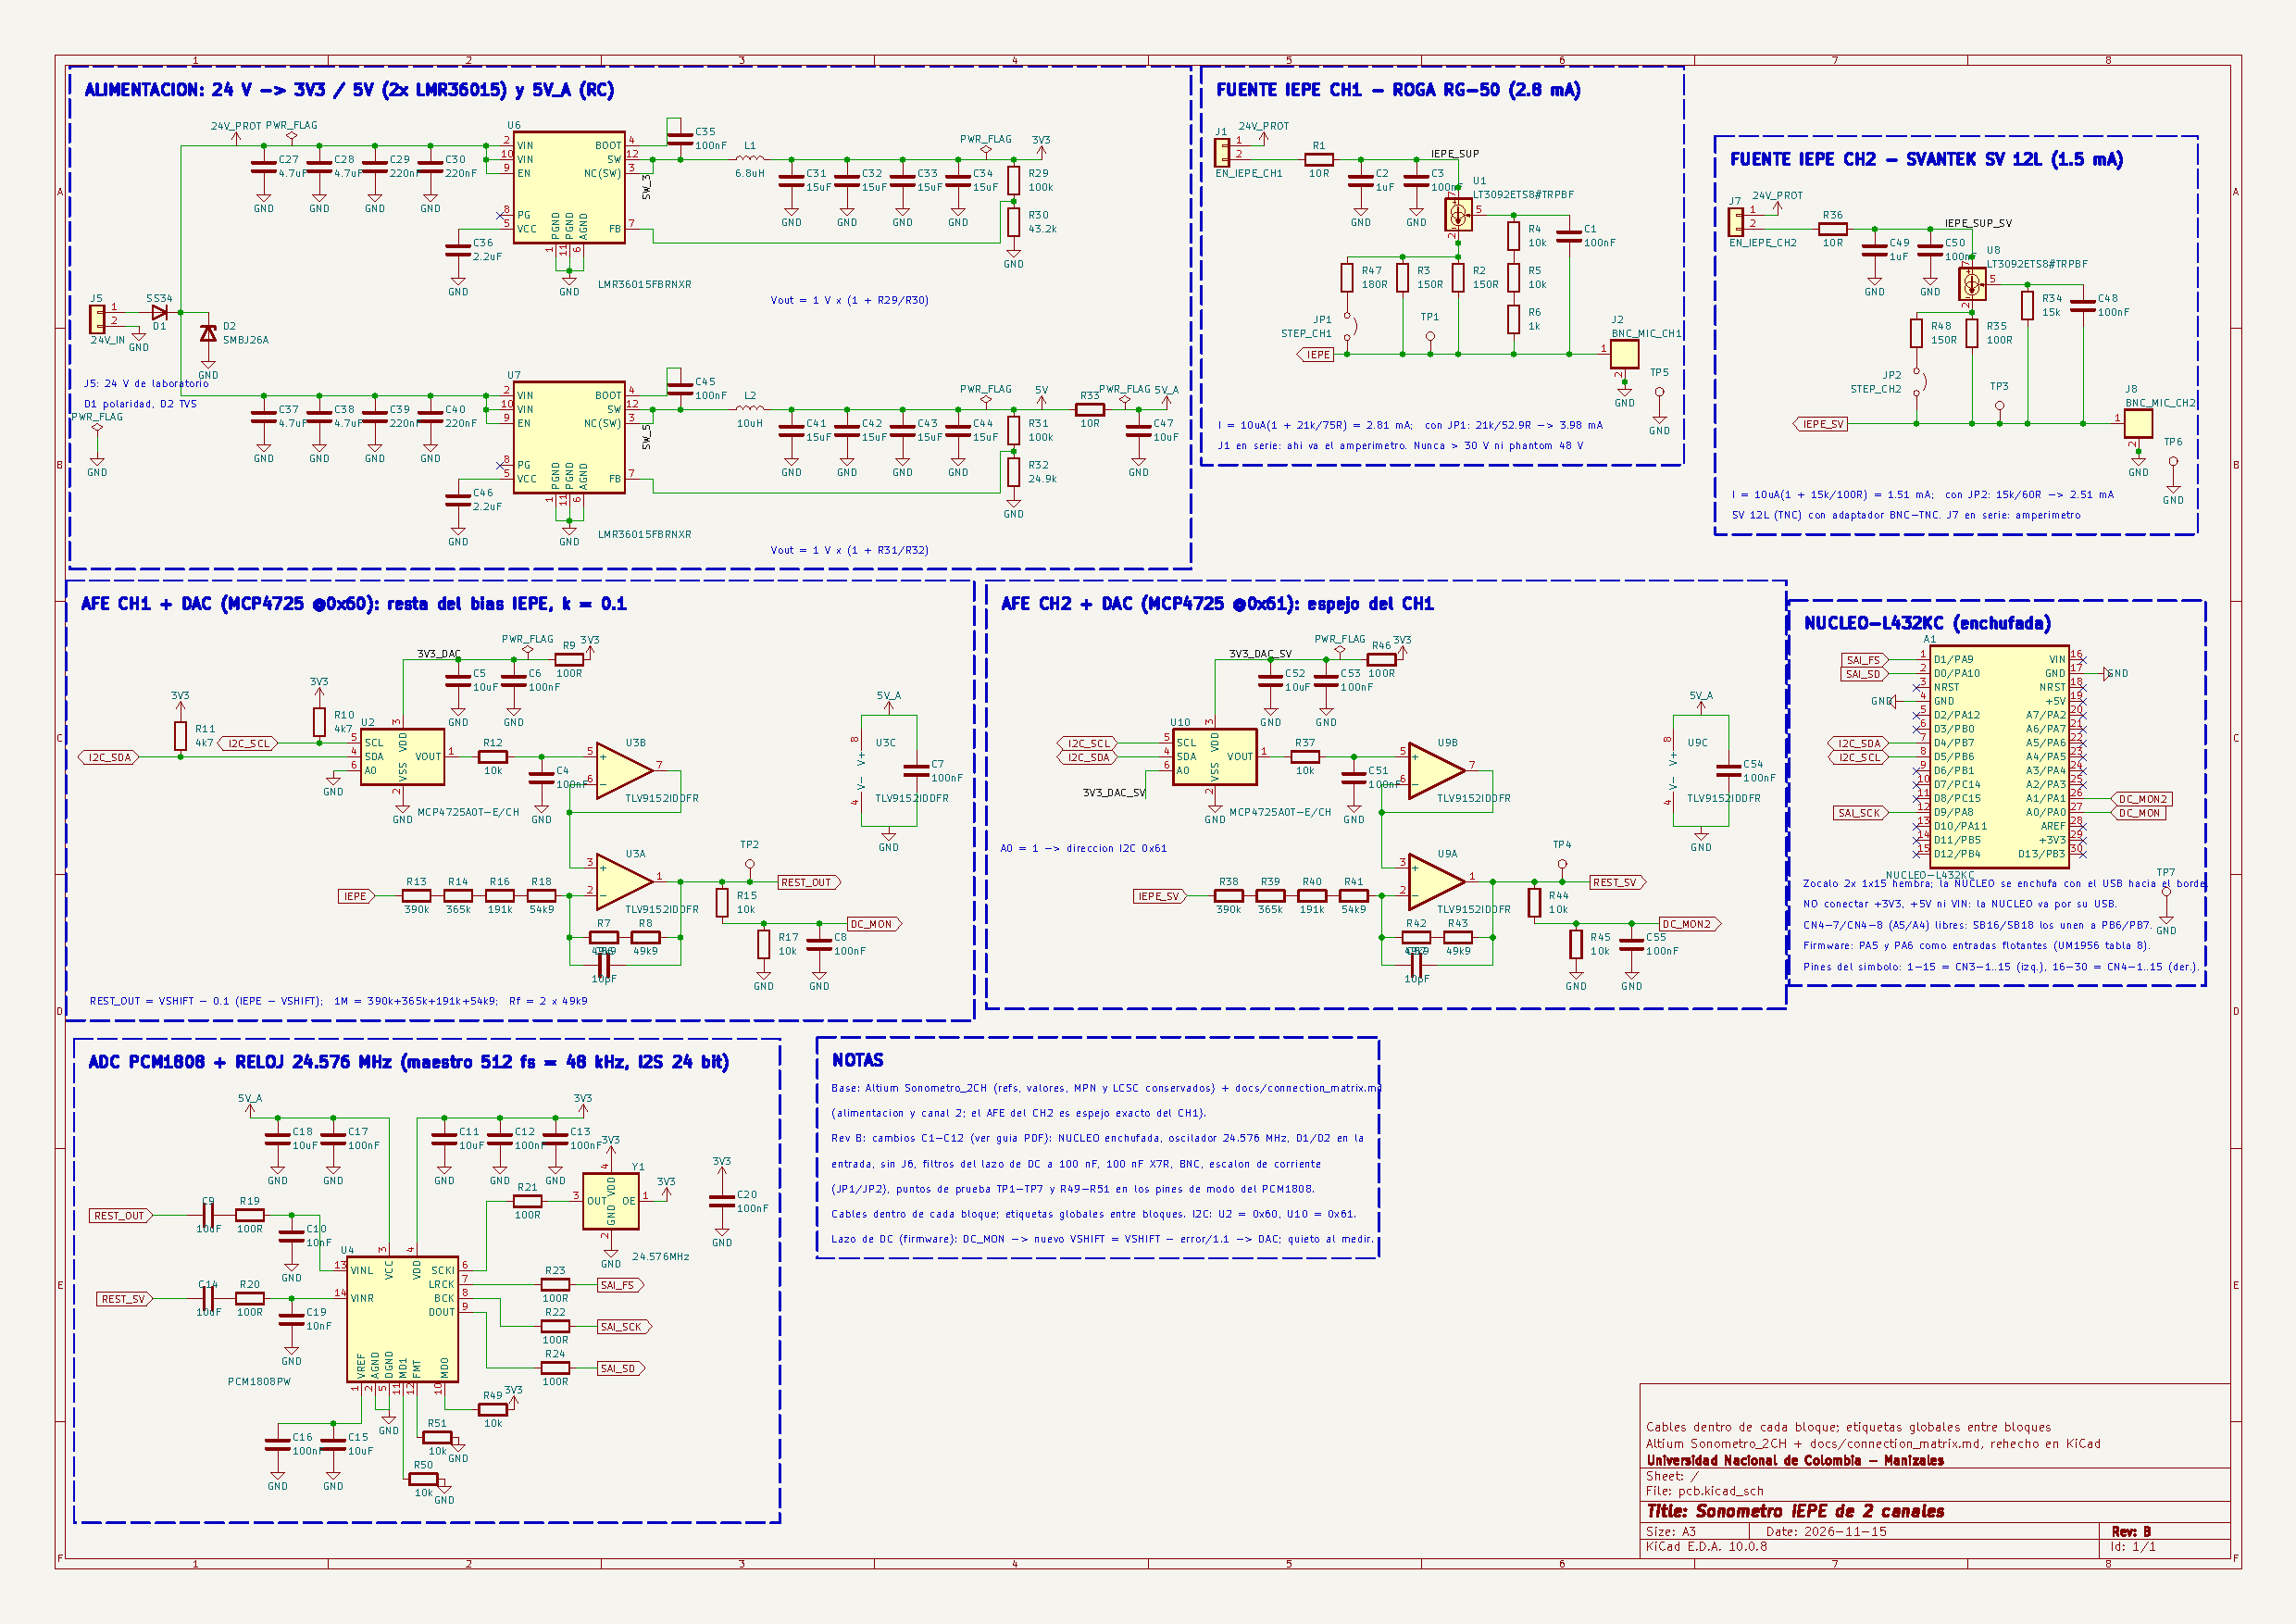
\includepdf[pages=-,landscape=true,scale=0.97]{figuras/esquematico.pdf}

\end{document}
